\documentclass[a4paper]{article}
\usepackage{makeidx}
\usepackage{natbib}
\usepackage{graphicx}
\usepackage{multicol}
\usepackage{float}
\usepackage{listings}
\usepackage{color}
\usepackage{ifthen}
\usepackage[table]{xcolor}
\usepackage{textcomp}
\usepackage{alltt}
\usepackage{ifpdf}
\ifpdf
\usepackage[pdftex,
            pagebackref=true,
            colorlinks=true,
            linkcolor=blue,
            unicode
           ]{hyperref}
\else
\usepackage[ps2pdf,
            pagebackref=true,
            colorlinks=true,
            linkcolor=blue,
            unicode
           ]{hyperref}
\usepackage{pspicture}
\fi
\usepackage[utf8]{inputenc}
\usepackage{mathptmx}
\usepackage[scaled=.90]{helvet}
\usepackage{courier}
\usepackage{sectsty}
\usepackage[titles]{tocloft}
\usepackage{doxygen}
\lstset{language=C++,inputencoding=utf8,basicstyle=\footnotesize,breaklines=true,breakatwhitespace=true,tabsize=4,numbers=left }
\makeindex
\setcounter{tocdepth}{3}
\renewcommand{\footrulewidth}{0.4pt}
\renewcommand{\familydefault}{\sfdefault}
\hfuzz=15pt
\setlength{\emergencystretch}{15pt}
\hbadness=750
\tolerance=750
\begin{document}
\hypersetup{pageanchor=false,citecolor=blue}
\begin{titlepage}
\vspace*{7cm}
\begin{center}
{\Large \-Ambient \-Light \-Transfer }\\
\vspace*{1cm}
{\large \-Generated by Doxygen 1.7.6.1}\\
\vspace*{0.5cm}
{\small Sun Sep 29 2013 22:37:51}\\
\end{center}
\end{titlepage}
\pagenumbering{roman}
\tableofcontents
\pagenumbering{arabic}
\hypersetup{pageanchor=true,citecolor=blue}
\section{\-Data \-Structure \-Index}
\subsection{\-Class \-Hierarchy}
\-This inheritance list is sorted roughly, but not completely, alphabetically\-:\begin{DoxyCompactList}
\item \contentsline{section}{\-Calibrate}{\pageref{classCalibrate}}{}
\item \contentsline{section}{\-Calibrate\-:\-:params}{\pageref{structCalibrate_1_1params}}{}
\item \contentsline{section}{circle}{\pageref{structcircle}}{}
\item \contentsline{section}{dir\-Cone}{\pageref{structdirCone}}{}
\item \contentsline{section}{\-Gui}{\pageref{classGui}}{}
\item \contentsline{section}{\-Image\-Source\-:\-:params}{\pageref{structImageSource_1_1params}}{}
\item \contentsline{section}{\-Lamps}{\pageref{classLamps}}{}
\begin{DoxyCompactList}
\item \contentsline{section}{\-Lamp\-Pool}{\pageref{classLampPool}}{}
\item \contentsline{section}{\-Sticks}{\pageref{classSticks}}{}
\item \contentsline{section}{\-Virtual\-Lamps}{\pageref{classVirtualLamps}}{}
\end{DoxyCompactList}
\item \contentsline{section}{\-Lightprobe}{\pageref{classLightprobe}}{}
\item \contentsline{section}{\-Lightprobe\-:\-:params}{\pageref{structLightprobe_1_1params}}{}
\item \contentsline{section}{\-Lightprobe\-:\-:sampling\-Params}{\pageref{structLightprobe_1_1samplingParams}}{}
\item \contentsline{section}{\-Log}{\pageref{classLog}}{}
\item \contentsline{section}{\-Max\-Exposure}{\pageref{classMaxExposure}}{}
\item \contentsline{section}{point}{\pageref{structpoint}}{}
\item \contentsline{section}{rect}{\pageref{structrect}}{}
\item \contentsline{section}{rgb}{\pageref{structrgb}}{}
\item \contentsline{section}{\-Sandbox}{\pageref{classSandbox}}{}
\item \contentsline{section}{\-Source}{\pageref{classSource}}{}
\begin{DoxyCompactList}
\item \contentsline{section}{\-Image\-Source}{\pageref{classImageSource}}{}
\item \contentsline{section}{\-X11\-Source}{\pageref{classX11Source}}{}
\end{DoxyCompactList}
\item \contentsline{section}{\-Sticks\-:\-:params}{\pageref{structSticks_1_1params}}{}
\item \contentsline{section}{\-Test\-Lamps}{\pageref{classTestLamps}}{}
\item \contentsline{section}{\-Test\-Probe}{\pageref{classTestProbe}}{}
\item \contentsline{section}{\-Transfer}{\pageref{classTransfer}}{}
\item \contentsline{section}{\-Transfer\-:\-:\-Cost\-Simple}{\pageref{classTransfer_1_1CostSimple}}{}
\item \contentsline{section}{\-Transfer\-:\-:params}{\pageref{structTransfer_1_1params}}{}
\item \contentsline{section}{\-Transfer\-:\-:\-Residual}{\pageref{structTransfer_1_1Residual}}{}
\item \contentsline{section}{\-X11\-Source\-:\-:params}{\pageref{structX11Source_1_1params}}{}
\end{DoxyCompactList}

\section{\-Data \-Structure \-Index}
\subsection{\-Data \-Structures}
\-Here are the data structures with brief descriptions\-:\begin{DoxyCompactList}
\item\contentsline{section}{\hyperlink{classCalibrate}{\-Calibrate} \\*\-The \-Calibration \-Loop }{\pageref{classCalibrate}}{}
\item\contentsline{section}{\hyperlink{structCalibrate_1_1params}{\-Calibrate\-::params} \\*\-Configuration of \hyperlink{classCalibrate}{\-Calibrate} class }{\pageref{structCalibrate_1_1params}}{}
\item\contentsline{section}{\hyperlink{structcircle}{circle} \\*\-A circle }{\pageref{structcircle}}{}
\item\contentsline{section}{\hyperlink{structdirCone}{dir\-Cone} \\*\-Stores the neighborhood of one sampling direction }{\pageref{structdirCone}}{}
\item\contentsline{section}{\hyperlink{classGui}{\-Gui} \\*\-The user interface }{\pageref{classGui}}{}
\item\contentsline{section}{\hyperlink{classImageSource}{\-Image\-Source} \\*\hyperlink{classSource}{\-Source} that uses image files }{\pageref{classImageSource}}{}
\item\contentsline{section}{\hyperlink{structImageSource_1_1params}{\-Image\-Source\-::params} \\*\-Configuration of the \hyperlink{classImageSource}{\-Image\-Source} class }{\pageref{structImageSource_1_1params}}{}
\item\contentsline{section}{\hyperlink{classLampPool}{\-Lamp\-Pool} \\*\-Groups instances of \hyperlink{classLamps}{\-Lamps} }{\pageref{classLampPool}}{}
\item\contentsline{section}{\hyperlink{classLamps}{\-Lamps} \\*\-A monochrome lamp }{\pageref{classLamps}}{}
\item\contentsline{section}{\hyperlink{classLightprobe}{\-Lightprobe} \\*\-Our light probe model }{\pageref{classLightprobe}}{}
\item\contentsline{section}{\hyperlink{structLightprobe_1_1params}{\-Lightprobe\-::params} \\*\-Configuration of the light probe }{\pageref{structLightprobe_1_1params}}{}
\item\contentsline{section}{\hyperlink{structLightprobe_1_1samplingParams}{\-Lightprobe\-::sampling\-Params} \\*\-Configures sampling }{\pageref{structLightprobe_1_1samplingParams}}{}
\item\contentsline{section}{\hyperlink{classLog}{\-Log} \\*\-A simple logger }{\pageref{classLog}}{}
\item\contentsline{section}{\hyperlink{classMaxExposure}{\-Max\-Exposure} \\*\-Adjusts the \-Exposure of a \-U\-V\-C webcam }{\pageref{classMaxExposure}}{}
\item\contentsline{section}{\hyperlink{structpoint}{point} \\*\-A point }{\pageref{structpoint}}{}
\item\contentsline{section}{\hyperlink{structrect}{rect} \\*\-A rectangle }{\pageref{structrect}}{}
\item\contentsline{section}{\hyperlink{structrgb}{rgb} \\*\-R\-G\-B color }{\pageref{structrgb}}{}
\item\contentsline{section}{\hyperlink{classSandbox}{\-Sandbox} \\*\-A sandbox for experiments }{\pageref{classSandbox}}{}
\item\contentsline{section}{\hyperlink{classSource}{\-Source} \\*\-Acquires and linearizes images }{\pageref{classSource}}{}
\item\contentsline{section}{\hyperlink{classSticks}{\-Sticks} \\*\-Our sticks lighting system }{\pageref{classSticks}}{}
\item\contentsline{section}{\hyperlink{structSticks_1_1params}{\-Sticks\-::params} \\*\-Configuration of our lighting system }{\pageref{structSticks_1_1params}}{}
\item\contentsline{section}{\hyperlink{classTestLamps}{\-Test\-Lamps} \\*\-Test lamps (for debug) }{\pageref{classTestLamps}}{}
\item\contentsline{section}{\hyperlink{classTestProbe}{\-Test\-Probe} \\*\-Test light probe (for debug) }{\pageref{classTestProbe}}{}
\item\contentsline{section}{\hyperlink{classTransfer}{\-Transfer} \\*\-The \-Ambient \-Light \hyperlink{classTransfer}{\-Transfer} loop }{\pageref{classTransfer}}{}
\item\contentsline{section}{\hyperlink{classTransfer_1_1CostSimple}{\-Transfer\-::\-Cost\-Simple} \\*\-Faster \-Cost\-Function for ceres }{\pageref{classTransfer_1_1CostSimple}}{}
\item\contentsline{section}{\hyperlink{structTransfer_1_1params}{\-Transfer\-::params} \\*\-Configuration }{\pageref{structTransfer_1_1params}}{}
\item\contentsline{section}{\hyperlink{structTransfer_1_1Residual}{\-Transfer\-::\-Residual} \\*\-Cost\-Function for ceres }{\pageref{structTransfer_1_1Residual}}{}
\item\contentsline{section}{\hyperlink{classVirtualLamps}{\-Virtual\-Lamps} \\*\hyperlink{classLamps}{\-Lamps} w/o hardware backend }{\pageref{classVirtualLamps}}{}
\item\contentsline{section}{\hyperlink{classX11Source}{\-X11\-Source} \\*\-X11 desktop grabber }{\pageref{classX11Source}}{}
\item\contentsline{section}{\hyperlink{structX11Source_1_1params}{\-X11\-Source\-::params} \\*\-Configuration of \hyperlink{classX11Source}{\-X11\-Source} }{\pageref{structX11Source_1_1params}}{}
\end{DoxyCompactList}

\section{\-File \-Index}
\subsection{\-File \-List}
\-Here is a list of all files with brief descriptions\-:\begin{DoxyCompactList}
\item\contentsline{section}{src/\hyperlink{alt_8cpp}{alt.\-cpp} }{\pageref{alt_8cpp}}{}
\item\contentsline{section}{src/\hyperlink{alt_8h}{alt.\-h} }{\pageref{alt_8h}}{}
\item\contentsline{section}{src/\hyperlink{calibrate_8cpp}{calibrate.\-cpp} }{\pageref{calibrate_8cpp}}{}
\item\contentsline{section}{src/\hyperlink{calibrate_8h}{calibrate.\-h} }{\pageref{calibrate_8h}}{}
\item\contentsline{section}{src/\hyperlink{gui_8cpp}{gui.\-cpp} }{\pageref{gui_8cpp}}{}
\item\contentsline{section}{src/\hyperlink{gui_8h}{gui.\-h} }{\pageref{gui_8h}}{}
\item\contentsline{section}{src/\hyperlink{imagesource_8cpp}{imagesource.\-cpp} }{\pageref{imagesource_8cpp}}{}
\item\contentsline{section}{src/\hyperlink{imagesource_8h}{imagesource.\-h} }{\pageref{imagesource_8h}}{}
\item\contentsline{section}{src/\hyperlink{lamppool_8cpp}{lamppool.\-cpp} }{\pageref{lamppool_8cpp}}{}
\item\contentsline{section}{src/\hyperlink{lamppool_8h}{lamppool.\-h} }{\pageref{lamppool_8h}}{}
\item\contentsline{section}{src/\hyperlink{lamps_8cpp}{lamps.\-cpp} }{\pageref{lamps_8cpp}}{}
\item\contentsline{section}{src/\hyperlink{lamps_8h}{lamps.\-h} }{\pageref{lamps_8h}}{}
\item\contentsline{section}{src/\hyperlink{lightprobe_8cpp}{lightprobe.\-cpp} }{\pageref{lightprobe_8cpp}}{}
\item\contentsline{section}{src/\hyperlink{lightprobe_8h}{lightprobe.\-h} }{\pageref{lightprobe_8h}}{}
\item\contentsline{section}{src/\hyperlink{maxexposure_8cpp}{maxexposure.\-cpp} }{\pageref{maxexposure_8cpp}}{}
\item\contentsline{section}{src/\hyperlink{maxexposure_8h}{maxexposure.\-h} }{\pageref{maxexposure_8h}}{}
\item\contentsline{section}{src/\hyperlink{sandbox_8cpp}{sandbox.\-cpp} }{\pageref{sandbox_8cpp}}{}
\item\contentsline{section}{src/\hyperlink{sandbox_8h}{sandbox.\-h} }{\pageref{sandbox_8h}}{}
\item\contentsline{section}{src/\hyperlink{source_8cpp}{source.\-cpp} }{\pageref{source_8cpp}}{}
\item\contentsline{section}{src/\hyperlink{source_8h}{source.\-h} }{\pageref{source_8h}}{}
\item\contentsline{section}{src/\hyperlink{sticks_8cpp}{sticks.\-cpp} }{\pageref{sticks_8cpp}}{}
\item\contentsline{section}{src/\hyperlink{sticks_8h}{sticks.\-h} }{\pageref{sticks_8h}}{}
\item\contentsline{section}{src/\hyperlink{testlamps_8cpp}{testlamps.\-cpp} }{\pageref{testlamps_8cpp}}{}
\item\contentsline{section}{src/\hyperlink{testlamps_8h}{testlamps.\-h} }{\pageref{testlamps_8h}}{}
\item\contentsline{section}{src/\hyperlink{testprobe_8cpp}{testprobe.\-cpp} }{\pageref{testprobe_8cpp}}{}
\item\contentsline{section}{src/\hyperlink{testprobe_8h}{testprobe.\-h} }{\pageref{testprobe_8h}}{}
\item\contentsline{section}{src/\hyperlink{transfer_8cpp}{transfer.\-cpp} }{\pageref{transfer_8cpp}}{}
\item\contentsline{section}{src/\hyperlink{transfer_8h}{transfer.\-h} }{\pageref{transfer_8h}}{}
\item\contentsline{section}{src/\hyperlink{utils_8cpp}{utils.\-cpp} }{\pageref{utils_8cpp}}{}
\item\contentsline{section}{src/\hyperlink{utils_8h}{utils.\-h} }{\pageref{utils_8h}}{}
\item\contentsline{section}{src/\hyperlink{virtuallamps_8cpp}{virtuallamps.\-cpp} }{\pageref{virtuallamps_8cpp}}{}
\item\contentsline{section}{src/\hyperlink{virtuallamps_8h}{virtuallamps.\-h} }{\pageref{virtuallamps_8h}}{}
\item\contentsline{section}{src/\hyperlink{x11source_8cpp}{x11source.\-cpp} }{\pageref{x11source_8cpp}}{}
\item\contentsline{section}{src/\hyperlink{x11source_8h}{x11source.\-h} }{\pageref{x11source_8h}}{}
\end{DoxyCompactList}

\section{\-Data \-Structure \-Documentation}
\hypertarget{classCalibrate}{\subsection{\-Calibrate \-Class \-Reference}
\label{classCalibrate}\index{\-Calibrate@{\-Calibrate}}
}


\-The \-Calibration \-Loop.  




{\ttfamily \#include $<$calibrate.\-h$>$}

\subsubsection*{\-Data \-Structures}
\begin{DoxyCompactItemize}
\item 
struct \hyperlink{structCalibrate_1_1params}{params}
\begin{DoxyCompactList}\small\item\em \-Configuration of \hyperlink{classCalibrate}{\-Calibrate} class. \end{DoxyCompactList}\end{DoxyCompactItemize}
\subsubsection*{\-Public \-Member \-Functions}
\begin{DoxyCompactItemize}
\item 
\hyperlink{classCalibrate_a9f1cb2fb9e76db3a4de6cc6a41f8225e}{\-Calibrate} (\hyperlink{classLightprobe}{\-Lightprobe} $\ast$p, \hyperlink{classLamps}{\-Lamps} $\ast$l, \hyperlink{structCalibrate_1_1params}{params} c)
\item 
\hyperlink{classCalibrate_ad1f6a92216d8cf4d49f1743f1e8d8cba}{\-Calibrate} (\hyperlink{classLightprobe}{\-Lightprobe} $\ast$p, \hyperlink{classLamps}{\-Lamps} $\ast$l, string path, double rate)
\item 
\hyperlink{classCalibrate_aa4cf6065d18ea089c23ba5de42f4da35}{$\sim$\-Calibrate} ()
\item 
\hyperlink{structCalibrate_1_1params}{params} \hyperlink{classCalibrate_a2050ebc8df9ad784c02b781a0634d7ca}{get\-Config} ()
\item 
void \hyperlink{classCalibrate_a4b635bcad3bf540a43fe01b47e54ad08}{run\-Capture\-Impacts} ()
\item 
void \hyperlink{classCalibrate_a9cce7906e90041efded1c24e6f5e14eb}{run\-Calibrate\-Lamps} ()
\end{DoxyCompactItemize}
\subsubsection*{\-Private \-Attributes}
\begin{DoxyCompactItemize}
\item 
\hyperlink{structCalibrate_1_1params}{params} \hyperlink{classCalibrate_ab03f352d65f3ad6ae97d4706066b0ea2}{config}
\item 
\hyperlink{classLightprobe}{\-Lightprobe} $\ast$ \hyperlink{classCalibrate_a67a7afddb9f985155355c8d6705d4e63}{probe}
\item 
\hyperlink{classLamps}{\-Lamps} $\ast$ \hyperlink{classCalibrate_ad21c76042bc2ea7b864c049d5f3ef531}{lamps}
\end{DoxyCompactItemize}


\subsubsection{\-Detailed \-Description}
\-The \-Calibration \-Loop. 

\begin{DoxyAuthor}{\-Author}
\-Manuel \-Jerger $<$\href{mailto:nom@nomnom.de}{\tt nom@nomnom.\-de}$>$ \-The \-Calibration \-Loop for use with the webcam probe. \-Can also measure the response curve of our lighting system. 
\end{DoxyAuthor}


\subsubsection{\-Constructor \& \-Destructor \-Documentation}
\hypertarget{classCalibrate_a9f1cb2fb9e76db3a4de6cc6a41f8225e}{\index{\-Calibrate@{\-Calibrate}!\-Calibrate@{\-Calibrate}}
\index{\-Calibrate@{\-Calibrate}!Calibrate@{\-Calibrate}}
\paragraph[{\-Calibrate}]{\setlength{\rightskip}{0pt plus 5cm}{\bf \-Calibrate\-::\-Calibrate} (
\begin{DoxyParamCaption}
\item[{{\bf \-Lightprobe} $\ast$}]{p, }
\item[{{\bf \-Lamps} $\ast$}]{l, }
\item[{{\bf params}}]{c}
\end{DoxyParamCaption}
)}}\label{classCalibrate_a9f1cb2fb9e76db3a4de6cc6a41f8225e}
\begin{DoxyAuthor}{\-Author}
\-Manuel \-Jerger $<$\href{mailto:nom@nomnom.de}{\tt nom@nomnom.\-de}$>$
\end{DoxyAuthor}
\-The \-Calibration \-Loop for use with the webcam probe. \-Can also measure the response curve of our lighting system. \hypertarget{classCalibrate_ad1f6a92216d8cf4d49f1743f1e8d8cba}{\index{\-Calibrate@{\-Calibrate}!\-Calibrate@{\-Calibrate}}
\index{\-Calibrate@{\-Calibrate}!Calibrate@{\-Calibrate}}
\paragraph[{\-Calibrate}]{\setlength{\rightskip}{0pt plus 5cm}{\bf \-Calibrate\-::\-Calibrate} (
\begin{DoxyParamCaption}
\item[{{\bf \-Lightprobe} $\ast$}]{p, }
\item[{{\bf \-Lamps} $\ast$}]{l, }
\item[{string}]{path, }
\item[{double}]{rate}
\end{DoxyParamCaption}
)}}\label{classCalibrate_ad1f6a92216d8cf4d49f1743f1e8d8cba}
\hypertarget{classCalibrate_aa4cf6065d18ea089c23ba5de42f4da35}{\index{\-Calibrate@{\-Calibrate}!$\sim$\-Calibrate@{$\sim$\-Calibrate}}
\index{$\sim$\-Calibrate@{$\sim$\-Calibrate}!Calibrate@{\-Calibrate}}
\paragraph[{$\sim$\-Calibrate}]{\setlength{\rightskip}{0pt plus 5cm}{\bf \-Calibrate\-::$\sim$\-Calibrate} (
\begin{DoxyParamCaption}
{}
\end{DoxyParamCaption}
)}}\label{classCalibrate_aa4cf6065d18ea089c23ba5de42f4da35}


\subsubsection{\-Member \-Function \-Documentation}
\hypertarget{classCalibrate_a2050ebc8df9ad784c02b781a0634d7ca}{\index{\-Calibrate@{\-Calibrate}!get\-Config@{get\-Config}}
\index{get\-Config@{get\-Config}!Calibrate@{\-Calibrate}}
\paragraph[{get\-Config}]{\setlength{\rightskip}{0pt plus 5cm}{\bf \-Calibrate\-::params} {\bf \-Calibrate\-::get\-Config} (
\begin{DoxyParamCaption}
{}
\end{DoxyParamCaption}
)}}\label{classCalibrate_a2050ebc8df9ad784c02b781a0634d7ca}
\hypertarget{classCalibrate_a9cce7906e90041efded1c24e6f5e14eb}{\index{\-Calibrate@{\-Calibrate}!run\-Calibrate\-Lamps@{run\-Calibrate\-Lamps}}
\index{run\-Calibrate\-Lamps@{run\-Calibrate\-Lamps}!Calibrate@{\-Calibrate}}
\paragraph[{run\-Calibrate\-Lamps}]{\setlength{\rightskip}{0pt plus 5cm}void {\bf \-Calibrate\-::run\-Calibrate\-Lamps} (
\begin{DoxyParamCaption}
{}
\end{DoxyParamCaption}
)}}\label{classCalibrate_a9cce7906e90041efded1c24e6f5e14eb}
\-Run the \-Lamp-\/\-Calibration and calculate \-L\-E\-D response using an image source and prerecorded images. \hypertarget{classCalibrate_a4b635bcad3bf540a43fe01b47e54ad08}{\index{\-Calibrate@{\-Calibrate}!run\-Capture\-Impacts@{run\-Capture\-Impacts}}
\index{run\-Capture\-Impacts@{run\-Capture\-Impacts}!Calibrate@{\-Calibrate}}
\paragraph[{run\-Capture\-Impacts}]{\setlength{\rightskip}{0pt plus 5cm}void {\bf \-Calibrate\-::run\-Capture\-Impacts} (
\begin{DoxyParamCaption}
{}
\end{DoxyParamCaption}
)}}\label{classCalibrate_a4b635bcad3bf540a43fe01b47e54ad08}
\-Run the calibration loop using the webcam. 

\subsubsection{\-Field \-Documentation}
\hypertarget{classCalibrate_ab03f352d65f3ad6ae97d4706066b0ea2}{\index{\-Calibrate@{\-Calibrate}!config@{config}}
\index{config@{config}!Calibrate@{\-Calibrate}}
\paragraph[{config}]{\setlength{\rightskip}{0pt plus 5cm}{\bf params} {\bf \-Calibrate\-::config}\hspace{0.3cm}{\ttfamily  \mbox{[}private\mbox{]}}}}\label{classCalibrate_ab03f352d65f3ad6ae97d4706066b0ea2}
\hypertarget{classCalibrate_ad21c76042bc2ea7b864c049d5f3ef531}{\index{\-Calibrate@{\-Calibrate}!lamps@{lamps}}
\index{lamps@{lamps}!Calibrate@{\-Calibrate}}
\paragraph[{lamps}]{\setlength{\rightskip}{0pt plus 5cm}{\bf \-Lamps}$\ast$ {\bf \-Calibrate\-::lamps}\hspace{0.3cm}{\ttfamily  \mbox{[}private\mbox{]}}}}\label{classCalibrate_ad21c76042bc2ea7b864c049d5f3ef531}
\hypertarget{classCalibrate_a67a7afddb9f985155355c8d6705d4e63}{\index{\-Calibrate@{\-Calibrate}!probe@{probe}}
\index{probe@{probe}!Calibrate@{\-Calibrate}}
\paragraph[{probe}]{\setlength{\rightskip}{0pt plus 5cm}{\bf \-Lightprobe}$\ast$ {\bf \-Calibrate\-::probe}\hspace{0.3cm}{\ttfamily  \mbox{[}private\mbox{]}}}}\label{classCalibrate_a67a7afddb9f985155355c8d6705d4e63}


\-The documentation for this class was generated from the following files\-:\begin{DoxyCompactItemize}
\item 
src/\hyperlink{calibrate_8h}{calibrate.\-h}\item 
src/\hyperlink{calibrate_8cpp}{calibrate.\-cpp}\end{DoxyCompactItemize}

\hypertarget{structCalibrate_1_1params}{\subsection{\-Calibrate\-:\-:params \-Struct \-Reference}
\label{structCalibrate_1_1params}\index{\-Calibrate\-::params@{\-Calibrate\-::params}}
}


\-Configuration of \hyperlink{classCalibrate}{\-Calibrate} class.  




{\ttfamily \#include $<$calibrate.\-h$>$}

\subsubsection*{\-Public \-Member \-Functions}
\begin{DoxyCompactItemize}
\item 
\hyperlink{structCalibrate_1_1params_a2533614061a9fc467b1123a8eb587471}{params} ()
\end{DoxyCompactItemize}
\subsubsection*{\-Data \-Fields}
\begin{DoxyCompactItemize}
\item 
string \hyperlink{structCalibrate_1_1params_a132084ddaaaf07b9687da1c6cb508726}{data\-Dir}
\item 
double \hyperlink{structCalibrate_1_1params_a56c34ddc4c233c7fe1d42b9f28c712ed}{capture\-Rate}
\end{DoxyCompactItemize}


\subsubsection{\-Detailed \-Description}
\-Configuration of \hyperlink{classCalibrate}{\-Calibrate} class. 

\subsubsection{\-Constructor \& \-Destructor \-Documentation}
\hypertarget{structCalibrate_1_1params_a2533614061a9fc467b1123a8eb587471}{\index{\-Calibrate\-::params@{\-Calibrate\-::params}!params@{params}}
\index{params@{params}!Calibrate::params@{\-Calibrate\-::params}}
\paragraph[{params}]{\setlength{\rightskip}{0pt plus 5cm}{\bf \-Calibrate\-::params\-::params} (
\begin{DoxyParamCaption}
{}
\end{DoxyParamCaption}
)\hspace{0.3cm}{\ttfamily  \mbox{[}inline\mbox{]}}}}\label{structCalibrate_1_1params_a2533614061a9fc467b1123a8eb587471}


\subsubsection{\-Field \-Documentation}
\hypertarget{structCalibrate_1_1params_a56c34ddc4c233c7fe1d42b9f28c712ed}{\index{\-Calibrate\-::params@{\-Calibrate\-::params}!capture\-Rate@{capture\-Rate}}
\index{capture\-Rate@{capture\-Rate}!Calibrate::params@{\-Calibrate\-::params}}
\paragraph[{capture\-Rate}]{\setlength{\rightskip}{0pt plus 5cm}double {\bf \-Calibrate\-::params\-::capture\-Rate}}}\label{structCalibrate_1_1params_a56c34ddc4c233c7fe1d42b9f28c712ed}
\hypertarget{structCalibrate_1_1params_a132084ddaaaf07b9687da1c6cb508726}{\index{\-Calibrate\-::params@{\-Calibrate\-::params}!data\-Dir@{data\-Dir}}
\index{data\-Dir@{data\-Dir}!Calibrate::params@{\-Calibrate\-::params}}
\paragraph[{data\-Dir}]{\setlength{\rightskip}{0pt plus 5cm}string {\bf \-Calibrate\-::params\-::data\-Dir}}}\label{structCalibrate_1_1params_a132084ddaaaf07b9687da1c6cb508726}


\-The documentation for this struct was generated from the following file\-:\begin{DoxyCompactItemize}
\item 
src/\hyperlink{calibrate_8h}{calibrate.\-h}\end{DoxyCompactItemize}

\hypertarget{structcircle}{\subsection{circle \-Struct \-Reference}
\label{structcircle}\index{circle@{circle}}
}


\-A circle.  




{\ttfamily \#include $<$utils.\-h$>$}

\subsubsection*{\-Public \-Member \-Functions}
\begin{DoxyCompactItemize}
\item 
\hyperlink{structcircle_a47cfe4c636835410b292a9f1fda841db}{circle} (double \hyperlink{structcircle_a3ecd01f4a611905b29614e61d8c6f068}{x}, double \hyperlink{structcircle_ac060cb1d497b470df6be2d4242369f31}{y}, double \hyperlink{structcircle_a5f252f6cf93b81949dbf334c74931f18}{r})
\item 
\hyperlink{structcircle_a4e0786fc75051f3bbe5de2e08ef9712d}{circle} ()
\item 
bool \hyperlink{structcircle_a103b7ebfdcb2da15c9a19f1e0ecb44a1}{is\-Valid} ()
\end{DoxyCompactItemize}
\subsubsection*{\-Data \-Fields}
\begin{DoxyCompactItemize}
\item 
double \hyperlink{structcircle_a3ecd01f4a611905b29614e61d8c6f068}{x}
\item 
double \hyperlink{structcircle_ac060cb1d497b470df6be2d4242369f31}{y}
\item 
double \hyperlink{structcircle_a5f252f6cf93b81949dbf334c74931f18}{r}
\end{DoxyCompactItemize}


\subsubsection{\-Detailed \-Description}
\-A circle. 

\subsubsection{\-Constructor \& \-Destructor \-Documentation}
\hypertarget{structcircle_a47cfe4c636835410b292a9f1fda841db}{\index{circle@{circle}!circle@{circle}}
\index{circle@{circle}!circle@{circle}}
\paragraph[{circle}]{\setlength{\rightskip}{0pt plus 5cm}{\bf circle\-::circle} (
\begin{DoxyParamCaption}
\item[{double}]{x, }
\item[{double}]{y, }
\item[{double}]{r}
\end{DoxyParamCaption}
)\hspace{0.3cm}{\ttfamily  \mbox{[}inline\mbox{]}}}}\label{structcircle_a47cfe4c636835410b292a9f1fda841db}
\hypertarget{structcircle_a4e0786fc75051f3bbe5de2e08ef9712d}{\index{circle@{circle}!circle@{circle}}
\index{circle@{circle}!circle@{circle}}
\paragraph[{circle}]{\setlength{\rightskip}{0pt plus 5cm}{\bf circle\-::circle} (
\begin{DoxyParamCaption}
{}
\end{DoxyParamCaption}
)\hspace{0.3cm}{\ttfamily  \mbox{[}inline\mbox{]}}}}\label{structcircle_a4e0786fc75051f3bbe5de2e08ef9712d}


\subsubsection{\-Member \-Function \-Documentation}
\hypertarget{structcircle_a103b7ebfdcb2da15c9a19f1e0ecb44a1}{\index{circle@{circle}!is\-Valid@{is\-Valid}}
\index{is\-Valid@{is\-Valid}!circle@{circle}}
\paragraph[{is\-Valid}]{\setlength{\rightskip}{0pt plus 5cm}bool {\bf circle\-::is\-Valid} (
\begin{DoxyParamCaption}
{}
\end{DoxyParamCaption}
)\hspace{0.3cm}{\ttfamily  \mbox{[}inline\mbox{]}}}}\label{structcircle_a103b7ebfdcb2da15c9a19f1e0ecb44a1}


\subsubsection{\-Field \-Documentation}
\hypertarget{structcircle_a5f252f6cf93b81949dbf334c74931f18}{\index{circle@{circle}!r@{r}}
\index{r@{r}!circle@{circle}}
\paragraph[{r}]{\setlength{\rightskip}{0pt plus 5cm}double {\bf circle\-::r}}}\label{structcircle_a5f252f6cf93b81949dbf334c74931f18}
\hypertarget{structcircle_a3ecd01f4a611905b29614e61d8c6f068}{\index{circle@{circle}!x@{x}}
\index{x@{x}!circle@{circle}}
\paragraph[{x}]{\setlength{\rightskip}{0pt plus 5cm}double {\bf circle\-::x}}}\label{structcircle_a3ecd01f4a611905b29614e61d8c6f068}
\hypertarget{structcircle_ac060cb1d497b470df6be2d4242369f31}{\index{circle@{circle}!y@{y}}
\index{y@{y}!circle@{circle}}
\paragraph[{y}]{\setlength{\rightskip}{0pt plus 5cm}double {\bf circle\-::y}}}\label{structcircle_ac060cb1d497b470df6be2d4242369f31}


\-The documentation for this struct was generated from the following file\-:\begin{DoxyCompactItemize}
\item 
src/\hyperlink{utils_8h}{utils.\-h}\end{DoxyCompactItemize}

\hypertarget{structdirCone}{\subsection{dir\-Cone \-Struct \-Reference}
\label{structdirCone}\index{dir\-Cone@{dir\-Cone}}
}


\-Stores the neighborhood of one sampling direction.  




{\ttfamily \#include $<$utils.\-h$>$}

\subsubsection*{\-Public \-Member \-Functions}
\begin{DoxyCompactItemize}
\item 
\hyperlink{structdirCone_a62caac4a9d4d1290171df975aa8f0045}{dir\-Cone} ()
\item 
\hyperlink{structdirCone_ae11918c2e058cf830b6afac73b5b0d39}{dir\-Cone} (\-Vector3d dir)
\item 
void \hyperlink{structdirCone_a2b140af6d384486e933f91e770d2192f}{add} (\-Vector3d dir, \-Vector2i pixel, double weight)
\end{DoxyCompactItemize}
\subsubsection*{\-Data \-Fields}
\begin{DoxyCompactItemize}
\item 
\-Vector3d \hyperlink{structdirCone_ad89d1fbdcde77400f608cdb1f502842d}{direction}
\item 
\hyperlink{utils_8h_aac426d8086789d4d7e318436071c9754}{directions} \hyperlink{structdirCone_ae7bfc1b6c2a55a772e2f6d009dac449d}{dirs}
\item 
vector$<$ \-Vector2i $>$ \hyperlink{structdirCone_ae420701e1029a65d9b79998247985a02}{pixels}
\item 
vector$<$ double $>$ \hyperlink{structdirCone_a4771a6176536f25c585f664b76d69da0}{weights}
\item 
double \hyperlink{structdirCone_a36ba2b6825f43391cac3e7096fc912a9}{weight\-Sum}
\end{DoxyCompactItemize}


\subsubsection{\-Detailed \-Description}
\-Stores the neighborhood of one sampling direction. 

\subsubsection{\-Constructor \& \-Destructor \-Documentation}
\hypertarget{structdirCone_a62caac4a9d4d1290171df975aa8f0045}{\index{dir\-Cone@{dir\-Cone}!dir\-Cone@{dir\-Cone}}
\index{dir\-Cone@{dir\-Cone}!dirCone@{dir\-Cone}}
\paragraph[{dir\-Cone}]{\setlength{\rightskip}{0pt plus 5cm}{\bf dir\-Cone\-::dir\-Cone} (
\begin{DoxyParamCaption}
{}
\end{DoxyParamCaption}
)\hspace{0.3cm}{\ttfamily  \mbox{[}inline\mbox{]}}}}\label{structdirCone_a62caac4a9d4d1290171df975aa8f0045}
\hypertarget{structdirCone_ae11918c2e058cf830b6afac73b5b0d39}{\index{dir\-Cone@{dir\-Cone}!dir\-Cone@{dir\-Cone}}
\index{dir\-Cone@{dir\-Cone}!dirCone@{dir\-Cone}}
\paragraph[{dir\-Cone}]{\setlength{\rightskip}{0pt plus 5cm}{\bf dir\-Cone\-::dir\-Cone} (
\begin{DoxyParamCaption}
\item[{\-Vector3d}]{dir}
\end{DoxyParamCaption}
)\hspace{0.3cm}{\ttfamily  \mbox{[}inline\mbox{]}}}}\label{structdirCone_ae11918c2e058cf830b6afac73b5b0d39}


\subsubsection{\-Member \-Function \-Documentation}
\hypertarget{structdirCone_a2b140af6d384486e933f91e770d2192f}{\index{dir\-Cone@{dir\-Cone}!add@{add}}
\index{add@{add}!dirCone@{dir\-Cone}}
\paragraph[{add}]{\setlength{\rightskip}{0pt plus 5cm}void {\bf dir\-Cone\-::add} (
\begin{DoxyParamCaption}
\item[{\-Vector3d}]{dir, }
\item[{\-Vector2i}]{pixel, }
\item[{double}]{weight}
\end{DoxyParamCaption}
)\hspace{0.3cm}{\ttfamily  \mbox{[}inline\mbox{]}}}}\label{structdirCone_a2b140af6d384486e933f91e770d2192f}


\subsubsection{\-Field \-Documentation}
\hypertarget{structdirCone_ad89d1fbdcde77400f608cdb1f502842d}{\index{dir\-Cone@{dir\-Cone}!direction@{direction}}
\index{direction@{direction}!dirCone@{dir\-Cone}}
\paragraph[{direction}]{\setlength{\rightskip}{0pt plus 5cm}\-Vector3d {\bf dir\-Cone\-::direction}}}\label{structdirCone_ad89d1fbdcde77400f608cdb1f502842d}
\hypertarget{structdirCone_ae7bfc1b6c2a55a772e2f6d009dac449d}{\index{dir\-Cone@{dir\-Cone}!dirs@{dirs}}
\index{dirs@{dirs}!dirCone@{dir\-Cone}}
\paragraph[{dirs}]{\setlength{\rightskip}{0pt plus 5cm}{\bf directions} {\bf dir\-Cone\-::dirs}}}\label{structdirCone_ae7bfc1b6c2a55a772e2f6d009dac449d}
\hypertarget{structdirCone_ae420701e1029a65d9b79998247985a02}{\index{dir\-Cone@{dir\-Cone}!pixels@{pixels}}
\index{pixels@{pixels}!dirCone@{dir\-Cone}}
\paragraph[{pixels}]{\setlength{\rightskip}{0pt plus 5cm}vector$<$\-Vector2i$>$ {\bf dir\-Cone\-::pixels}}}\label{structdirCone_ae420701e1029a65d9b79998247985a02}
\hypertarget{structdirCone_a4771a6176536f25c585f664b76d69da0}{\index{dir\-Cone@{dir\-Cone}!weights@{weights}}
\index{weights@{weights}!dirCone@{dir\-Cone}}
\paragraph[{weights}]{\setlength{\rightskip}{0pt plus 5cm}vector$<$double$>$ {\bf dir\-Cone\-::weights}}}\label{structdirCone_a4771a6176536f25c585f664b76d69da0}
\hypertarget{structdirCone_a36ba2b6825f43391cac3e7096fc912a9}{\index{dir\-Cone@{dir\-Cone}!weight\-Sum@{weight\-Sum}}
\index{weight\-Sum@{weight\-Sum}!dirCone@{dir\-Cone}}
\paragraph[{weight\-Sum}]{\setlength{\rightskip}{0pt plus 5cm}double {\bf dir\-Cone\-::weight\-Sum}}}\label{structdirCone_a36ba2b6825f43391cac3e7096fc912a9}


\-The documentation for this struct was generated from the following file\-:\begin{DoxyCompactItemize}
\item 
src/\hyperlink{utils_8h}{utils.\-h}\end{DoxyCompactItemize}

\hypertarget{classGui}{\subsection{\-Gui \-Class \-Reference}
\label{classGui}\index{\-Gui@{\-Gui}}
}


\-The user interface.  




{\ttfamily \#include $<$gui.\-h$>$}

\subsubsection*{\-Public \-Member \-Functions}
\begin{DoxyCompactItemize}
\item 
\hyperlink{classGui_ab2655dbb6d3a91d7e90cb83dad6c0450}{\-Gui} ()
\item 
\hyperlink{classGui_af1c8c5496c641bf4bd8c0780fb3cc781}{\-Gui} (int width, int height)
\item 
\hyperlink{classGui_a4fd8485d226f9b8a2ac2d81d7f0f3598}{$\sim$\-Gui} ()
\item 
void \hyperlink{classGui_ab22584cbddc02490c1737caf6e20ee5a}{start} (int width, int height)
\item 
const void \hyperlink{classGui_a22030a241ba6e5ba6cbbc280da4a1d06}{draw\-Line} (\hyperlink{structpoint}{point} f, \hyperlink{structpoint}{point} t)
\item 
const void \hyperlink{classGui_aaac1baf43d5d651a1793af86073244c2}{draw\-Line} (int x1, int y1, int x2, int y2)
\item 
const void \hyperlink{classGui_afb53d164f934b70952fdb08334ef6e55}{draw\-Box} (\hyperlink{structrect}{rect} box)
\item 
const void \hyperlink{classGui_a88dc6f9d334da3e0c842260883ac679d}{draw\-Box} (int x1, int y1, int x2, int y2)
\item 
const void \hyperlink{classGui_a3507ef363af011a7d190373568246b5c}{draw\-Circle} (\hyperlink{structcircle}{circle} c)
\item 
const void \hyperlink{classGui_a9516c3534860be388decd0a1359b77a6}{draw\-Circle} (\hyperlink{structcircle}{circle} c, int x, int y)
\item 
const void \hyperlink{classGui_a162fc4d49a18dd268c650301b44c58c0}{draw\-Circle\-Filled} (int xpos, int ypos, int radius)
\item 
const void \hyperlink{classGui_a49607add54d254a375a67626aea14874}{draw\-Points} (vector$<$ \-Vector2i $>$)
\item 
const void \hyperlink{classGui_a890eb7e15ebcd27442265750289c8a1c}{draw\-Points} (vector$<$ \-Vector2i $>$, int x, int y)
\item 
const void \hyperlink{classGui_a2ed9c555b5222b97051925a05bfafe07}{draw\-Image} (imglib\-::\-Image$<$ float $>$ \&, int, int)
\item 
const void \hyperlink{classGui_abc6b714f3cb3071178896c53966ba3a7}{draw\-Image} (imglib\-::\-Image$<$ float $>$ \&img, int xpos, int ypos, bool is\-Linear)
\item 
const void \hyperlink{classGui_ac4cd3095167790347e76b706d9c176ab}{draw\-Circular\-Image} (imglib\-::\-Image$<$ float $>$ \&img, \hyperlink{structcircle}{circle}, int x, int y)
\item 
const void \hyperlink{classGui_a341d87fe70343f149606787c1f6389e4}{draw\-Circular\-Image} (imglib\-::\-Image$<$ float $>$ \&, \hyperlink{structcircle}{circle})
\item 
const void \hyperlink{classGui_a9cfedb7c38c95fd99de96d48dc25053a}{draw\-Stick\-R\-G\-B\-Grid} (\hyperlink{classLamps}{\-Lamps} $\ast$, int x, int y, int w, int h, int space, bool)
\item 
const void \hyperlink{classGui_acce05435c1f43bcd80a2ed8ddc216a87}{draw\-Monochrome\-Lamps} (\hyperlink{classLamps}{\-Lamps} $\ast$lamps, int x, int y, int box\-\_\-width, int box\-\_\-height, int space, bool vertical)
\item 
const \hyperlink{structcircle}{circle} \hyperlink{classGui_a969a83c1a030acb4254e7b58afc4dff8}{run\-Sphere\-Selection} (\hyperlink{classSource}{\-Source} $\ast$)
\item 
const \hyperlink{structpoint}{point} \hyperlink{classGui_a81d08ecea8196f17a8514e7e70cd5970}{run\-Pixel\-Selection} (\hyperlink{classSource}{\-Source} $\ast$)
\end{DoxyCompactItemize}


\subsubsection{\-Detailed \-Description}
\-The user interface. 

\begin{DoxyAuthor}{\-Author}
\-Manuel \-Jerger $<$\href{mailto:nom@nomnom.de}{\tt nom@nomnom.\-de}$>$
\end{DoxyAuthor}
\-The graphic user interface. \-Uses \-Open\-G\-L via the glfw abstraction layer. 

\subsubsection{\-Constructor \& \-Destructor \-Documentation}
\hypertarget{classGui_ab2655dbb6d3a91d7e90cb83dad6c0450}{\index{\-Gui@{\-Gui}!\-Gui@{\-Gui}}
\index{\-Gui@{\-Gui}!Gui@{\-Gui}}
\paragraph[{\-Gui}]{\setlength{\rightskip}{0pt plus 5cm}{\bf \-Gui\-::\-Gui} (
\begin{DoxyParamCaption}
{}
\end{DoxyParamCaption}
)\hspace{0.3cm}{\ttfamily  \mbox{[}inline\mbox{]}}}}\label{classGui_ab2655dbb6d3a91d7e90cb83dad6c0450}
\hypertarget{classGui_af1c8c5496c641bf4bd8c0780fb3cc781}{\index{\-Gui@{\-Gui}!\-Gui@{\-Gui}}
\index{\-Gui@{\-Gui}!Gui@{\-Gui}}
\paragraph[{\-Gui}]{\setlength{\rightskip}{0pt plus 5cm}{\bf \-Gui\-::\-Gui} (
\begin{DoxyParamCaption}
\item[{int}]{width, }
\item[{int}]{height}
\end{DoxyParamCaption}
)}}\label{classGui_af1c8c5496c641bf4bd8c0780fb3cc781}
\hypertarget{classGui_a4fd8485d226f9b8a2ac2d81d7f0f3598}{\index{\-Gui@{\-Gui}!$\sim$\-Gui@{$\sim$\-Gui}}
\index{$\sim$\-Gui@{$\sim$\-Gui}!Gui@{\-Gui}}
\paragraph[{$\sim$\-Gui}]{\setlength{\rightskip}{0pt plus 5cm}{\bf \-Gui\-::$\sim$\-Gui} (
\begin{DoxyParamCaption}
{}
\end{DoxyParamCaption}
)}}\label{classGui_a4fd8485d226f9b8a2ac2d81d7f0f3598}


\subsubsection{\-Member \-Function \-Documentation}
\hypertarget{classGui_afb53d164f934b70952fdb08334ef6e55}{\index{\-Gui@{\-Gui}!draw\-Box@{draw\-Box}}
\index{draw\-Box@{draw\-Box}!Gui@{\-Gui}}
\paragraph[{draw\-Box}]{\setlength{\rightskip}{0pt plus 5cm}const void {\bf \-Gui\-::draw\-Box} (
\begin{DoxyParamCaption}
\item[{{\bf rect}}]{box}
\end{DoxyParamCaption}
)}}\label{classGui_afb53d164f934b70952fdb08334ef6e55}
\hypertarget{classGui_a88dc6f9d334da3e0c842260883ac679d}{\index{\-Gui@{\-Gui}!draw\-Box@{draw\-Box}}
\index{draw\-Box@{draw\-Box}!Gui@{\-Gui}}
\paragraph[{draw\-Box}]{\setlength{\rightskip}{0pt plus 5cm}const void {\bf \-Gui\-::draw\-Box} (
\begin{DoxyParamCaption}
\item[{int}]{x1, }
\item[{int}]{y1, }
\item[{int}]{x2, }
\item[{int}]{y2}
\end{DoxyParamCaption}
)}}\label{classGui_a88dc6f9d334da3e0c842260883ac679d}
\hypertarget{classGui_a3507ef363af011a7d190373568246b5c}{\index{\-Gui@{\-Gui}!draw\-Circle@{draw\-Circle}}
\index{draw\-Circle@{draw\-Circle}!Gui@{\-Gui}}
\paragraph[{draw\-Circle}]{\setlength{\rightskip}{0pt plus 5cm}const void {\bf \-Gui\-::draw\-Circle} (
\begin{DoxyParamCaption}
\item[{{\bf circle}}]{c}
\end{DoxyParamCaption}
)}}\label{classGui_a3507ef363af011a7d190373568246b5c}
\hypertarget{classGui_a9516c3534860be388decd0a1359b77a6}{\index{\-Gui@{\-Gui}!draw\-Circle@{draw\-Circle}}
\index{draw\-Circle@{draw\-Circle}!Gui@{\-Gui}}
\paragraph[{draw\-Circle}]{\setlength{\rightskip}{0pt plus 5cm}const void {\bf \-Gui\-::draw\-Circle} (
\begin{DoxyParamCaption}
\item[{{\bf circle}}]{c, }
\item[{int}]{x, }
\item[{int}]{y}
\end{DoxyParamCaption}
)}}\label{classGui_a9516c3534860be388decd0a1359b77a6}
\hypertarget{classGui_a162fc4d49a18dd268c650301b44c58c0}{\index{\-Gui@{\-Gui}!draw\-Circle\-Filled@{draw\-Circle\-Filled}}
\index{draw\-Circle\-Filled@{draw\-Circle\-Filled}!Gui@{\-Gui}}
\paragraph[{draw\-Circle\-Filled}]{\setlength{\rightskip}{0pt plus 5cm}const void {\bf \-Gui\-::draw\-Circle\-Filled} (
\begin{DoxyParamCaption}
\item[{int}]{xpos, }
\item[{int}]{ypos, }
\item[{int}]{radius}
\end{DoxyParamCaption}
)}}\label{classGui_a162fc4d49a18dd268c650301b44c58c0}
\hypertarget{classGui_ac4cd3095167790347e76b706d9c176ab}{\index{\-Gui@{\-Gui}!draw\-Circular\-Image@{draw\-Circular\-Image}}
\index{draw\-Circular\-Image@{draw\-Circular\-Image}!Gui@{\-Gui}}
\paragraph[{draw\-Circular\-Image}]{\setlength{\rightskip}{0pt plus 5cm}const void {\bf \-Gui\-::draw\-Circular\-Image} (
\begin{DoxyParamCaption}
\item[{imglib\-::\-Image$<$ float $>$ \&}]{img, }
\item[{{\bf circle}}]{area, }
\item[{int}]{x, }
\item[{int}]{y}
\end{DoxyParamCaption}
)}}\label{classGui_ac4cd3095167790347e76b706d9c176ab}
\hypertarget{classGui_a341d87fe70343f149606787c1f6389e4}{\index{\-Gui@{\-Gui}!draw\-Circular\-Image@{draw\-Circular\-Image}}
\index{draw\-Circular\-Image@{draw\-Circular\-Image}!Gui@{\-Gui}}
\paragraph[{draw\-Circular\-Image}]{\setlength{\rightskip}{0pt plus 5cm}const void {\bf \-Gui\-::draw\-Circular\-Image} (
\begin{DoxyParamCaption}
\item[{imglib\-::\-Image$<$ float $>$ \&}]{img, }
\item[{{\bf circle}}]{area}
\end{DoxyParamCaption}
)}}\label{classGui_a341d87fe70343f149606787c1f6389e4}
\hypertarget{classGui_a2ed9c555b5222b97051925a05bfafe07}{\index{\-Gui@{\-Gui}!draw\-Image@{draw\-Image}}
\index{draw\-Image@{draw\-Image}!Gui@{\-Gui}}
\paragraph[{draw\-Image}]{\setlength{\rightskip}{0pt plus 5cm}const void {\bf \-Gui\-::draw\-Image} (
\begin{DoxyParamCaption}
\item[{imglib\-::\-Image$<$ float $>$ \&}]{img, }
\item[{int}]{xpos, }
\item[{int}]{ypos}
\end{DoxyParamCaption}
)}}\label{classGui_a2ed9c555b5222b97051925a05bfafe07}
\hypertarget{classGui_abc6b714f3cb3071178896c53966ba3a7}{\index{\-Gui@{\-Gui}!draw\-Image@{draw\-Image}}
\index{draw\-Image@{draw\-Image}!Gui@{\-Gui}}
\paragraph[{draw\-Image}]{\setlength{\rightskip}{0pt plus 5cm}const void {\bf \-Gui\-::draw\-Image} (
\begin{DoxyParamCaption}
\item[{imglib\-::\-Image$<$ float $>$ \&}]{img, }
\item[{int}]{xpos, }
\item[{int}]{ypos, }
\item[{bool}]{is\-Linear}
\end{DoxyParamCaption}
)}}\label{classGui_abc6b714f3cb3071178896c53966ba3a7}
\hypertarget{classGui_a22030a241ba6e5ba6cbbc280da4a1d06}{\index{\-Gui@{\-Gui}!draw\-Line@{draw\-Line}}
\index{draw\-Line@{draw\-Line}!Gui@{\-Gui}}
\paragraph[{draw\-Line}]{\setlength{\rightskip}{0pt plus 5cm}const void {\bf \-Gui\-::draw\-Line} (
\begin{DoxyParamCaption}
\item[{{\bf point}}]{f, }
\item[{{\bf point}}]{t}
\end{DoxyParamCaption}
)}}\label{classGui_a22030a241ba6e5ba6cbbc280da4a1d06}
\hypertarget{classGui_aaac1baf43d5d651a1793af86073244c2}{\index{\-Gui@{\-Gui}!draw\-Line@{draw\-Line}}
\index{draw\-Line@{draw\-Line}!Gui@{\-Gui}}
\paragraph[{draw\-Line}]{\setlength{\rightskip}{0pt plus 5cm}const void {\bf \-Gui\-::draw\-Line} (
\begin{DoxyParamCaption}
\item[{int}]{x1, }
\item[{int}]{y1, }
\item[{int}]{x2, }
\item[{int}]{y2}
\end{DoxyParamCaption}
)}}\label{classGui_aaac1baf43d5d651a1793af86073244c2}
\hypertarget{classGui_acce05435c1f43bcd80a2ed8ddc216a87}{\index{\-Gui@{\-Gui}!draw\-Monochrome\-Lamps@{draw\-Monochrome\-Lamps}}
\index{draw\-Monochrome\-Lamps@{draw\-Monochrome\-Lamps}!Gui@{\-Gui}}
\paragraph[{draw\-Monochrome\-Lamps}]{\setlength{\rightskip}{0pt plus 5cm}const void {\bf \-Gui\-::draw\-Monochrome\-Lamps} (
\begin{DoxyParamCaption}
\item[{{\bf \-Lamps} $\ast$}]{lamps, }
\item[{int}]{x, }
\item[{int}]{y, }
\item[{int}]{box\-\_\-width, }
\item[{int}]{box\-\_\-height, }
\item[{int}]{space, }
\item[{bool}]{vertical}
\end{DoxyParamCaption}
)}}\label{classGui_acce05435c1f43bcd80a2ed8ddc216a87}
\-Draw value of monochrome lamps as white rectangle. \hypertarget{classGui_a49607add54d254a375a67626aea14874}{\index{\-Gui@{\-Gui}!draw\-Points@{draw\-Points}}
\index{draw\-Points@{draw\-Points}!Gui@{\-Gui}}
\paragraph[{draw\-Points}]{\setlength{\rightskip}{0pt plus 5cm}const void {\bf \-Gui\-::draw\-Points} (
\begin{DoxyParamCaption}
\item[{vector$<$ \-Vector2i $>$}]{points}
\end{DoxyParamCaption}
)}}\label{classGui_a49607add54d254a375a67626aea14874}
\hypertarget{classGui_a890eb7e15ebcd27442265750289c8a1c}{\index{\-Gui@{\-Gui}!draw\-Points@{draw\-Points}}
\index{draw\-Points@{draw\-Points}!Gui@{\-Gui}}
\paragraph[{draw\-Points}]{\setlength{\rightskip}{0pt plus 5cm}const void {\bf \-Gui\-::draw\-Points} (
\begin{DoxyParamCaption}
\item[{vector$<$ \-Vector2i $>$}]{points, }
\item[{int}]{x, }
\item[{int}]{y}
\end{DoxyParamCaption}
)}}\label{classGui_a890eb7e15ebcd27442265750289c8a1c}
\hypertarget{classGui_a9cfedb7c38c95fd99de96d48dc25053a}{\index{\-Gui@{\-Gui}!draw\-Stick\-R\-G\-B\-Grid@{draw\-Stick\-R\-G\-B\-Grid}}
\index{draw\-Stick\-R\-G\-B\-Grid@{draw\-Stick\-R\-G\-B\-Grid}!Gui@{\-Gui}}
\paragraph[{draw\-Stick\-R\-G\-B\-Grid}]{\setlength{\rightskip}{0pt plus 5cm}const void {\bf \-Gui\-::draw\-Stick\-R\-G\-B\-Grid} (
\begin{DoxyParamCaption}
\item[{{\bf \-Lamps} $\ast$}]{lamps, }
\item[{int}]{x, }
\item[{int}]{y, }
\item[{int}]{box\-\_\-width, }
\item[{int}]{box\-\_\-height, }
\item[{int}]{space, }
\item[{bool}]{vertical}
\end{DoxyParamCaption}
)}}\label{classGui_a9cfedb7c38c95fd99de96d48dc25053a}
\-Draw the lamp's \-R\-G\-B values as a table of rectangles 
\begin{DoxyParams}{\-Parameters}
{\em x} & \-Top left position inside window. \\
\hline
{\em y} & \-Top left position inside window. \\
\hline
{\em box\-\_\-width} & \-Width of rectangle. \\
\hline
{\em box\-\_\-height} & \-Height of rectangle. \\
\hline
{\em space} & \-Spacing between rectangles. \\
\hline
{\em vertical} & \-Orientation \\
\hline
\end{DoxyParams}
\hypertarget{classGui_a81d08ecea8196f17a8514e7e70cd5970}{\index{\-Gui@{\-Gui}!run\-Pixel\-Selection@{run\-Pixel\-Selection}}
\index{run\-Pixel\-Selection@{run\-Pixel\-Selection}!Gui@{\-Gui}}
\paragraph[{run\-Pixel\-Selection}]{\setlength{\rightskip}{0pt plus 5cm}const {\bf point} {\bf \-Gui\-::run\-Pixel\-Selection} (
\begin{DoxyParamCaption}
\item[{{\bf \-Source} $\ast$}]{source}
\end{DoxyParamCaption}
)}}\label{classGui_a81d08ecea8196f17a8514e7e70cd5970}
\-Displays images acquired from source and asks user to select a pixel / 2\-D coordinate. 
\begin{DoxyParams}{\-Parameters}
{\em source} & \-Image source. \\
\hline
\end{DoxyParams}
\begin{DoxyReturn}{\-Returns}
\-The pixel position. 
\end{DoxyReturn}
\hypertarget{classGui_a969a83c1a030acb4254e7b58afc4dff8}{\index{\-Gui@{\-Gui}!run\-Sphere\-Selection@{run\-Sphere\-Selection}}
\index{run\-Sphere\-Selection@{run\-Sphere\-Selection}!Gui@{\-Gui}}
\paragraph[{run\-Sphere\-Selection}]{\setlength{\rightskip}{0pt plus 5cm}const {\bf circle} {\bf \-Gui\-::run\-Sphere\-Selection} (
\begin{DoxyParamCaption}
\item[{{\bf \-Source} $\ast$}]{source}
\end{DoxyParamCaption}
)}}\label{classGui_a969a83c1a030acb4254e7b58afc4dff8}
\-Displays images acquired from source and asks user to select a sphere by clicking three points on the border of a circle. 
\begin{DoxyParams}{\-Parameters}
{\em source} & \-Image source. \\
\hline
\end{DoxyParams}
\begin{DoxyReturn}{\-Returns}
\-The parameters of the circle. 
\end{DoxyReturn}
\hypertarget{classGui_ab22584cbddc02490c1737caf6e20ee5a}{\index{\-Gui@{\-Gui}!start@{start}}
\index{start@{start}!Gui@{\-Gui}}
\paragraph[{start}]{\setlength{\rightskip}{0pt plus 5cm}void {\bf \-Gui\-::start} (
\begin{DoxyParamCaption}
\item[{int}]{width, }
\item[{int}]{height}
\end{DoxyParamCaption}
)}}\label{classGui_ab22584cbddc02490c1737caf6e20ee5a}
\-Start the \-G\-U\-I with a specified window size. \-Sets up \-Open\-G\-L and displays the window.


\begin{DoxyParams}{\-Parameters}
{\em width} & \-Width of window in pixel. \\
\hline
{\em height} & \-Height of window in pixel. \\
\hline
\end{DoxyParams}


\-The documentation for this class was generated from the following files\-:\begin{DoxyCompactItemize}
\item 
src/\hyperlink{gui_8h}{gui.\-h}\item 
src/\hyperlink{gui_8cpp}{gui.\-cpp}\end{DoxyCompactItemize}

\hypertarget{classImageSource}{\subsection{\-Image\-Source \-Class \-Reference}
\label{classImageSource}\index{\-Image\-Source@{\-Image\-Source}}
}


\hyperlink{classSource}{\-Source} that uses image files.  




{\ttfamily \#include $<$imagesource.\-h$>$}

\-Inheritance diagram for \-Image\-Source\-:\begin{figure}[H]
\begin{center}
\leavevmode
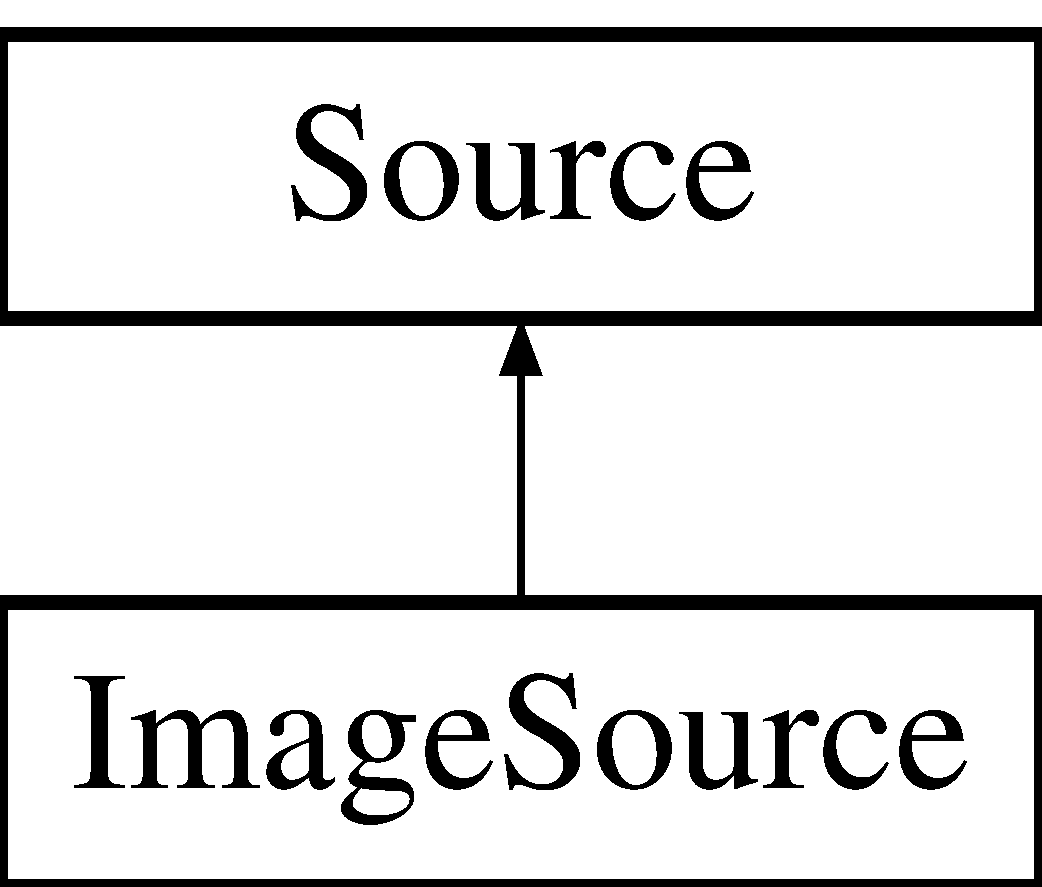
\includegraphics[height=2.000000cm]{classImageSource}
\end{center}
\end{figure}
\subsubsection*{\-Data \-Structures}
\begin{DoxyCompactItemize}
\item 
struct \hyperlink{structImageSource_1_1params}{params}
\begin{DoxyCompactList}\small\item\em \-Configuration of the \hyperlink{classImageSource}{\-Image\-Source} class. \end{DoxyCompactList}\end{DoxyCompactItemize}
\subsubsection*{\-Public \-Member \-Functions}
\begin{DoxyCompactItemize}
\item 
\hyperlink{classImageSource_a086ebf6a4094dc52b65b991b147b6c4d}{\-Image\-Source} (\hyperlink{structImageSource_1_1params}{params} c)
\item 
\hyperlink{classImageSource_a6b2d501403e70bb460ac337e68ee16d7}{$\sim$\-Image\-Source} ()
\item 
\hyperlink{structImageSource_1_1params}{params} \hyperlink{classImageSource_a7cc846a2611cc5a90296782d922041e8}{get\-Config} ()
\item 
bool \hyperlink{classImageSource_ab65bd864ba3c7961479ec2ad3b1ff163}{has\-New\-Data} ()
\item 
void \hyperlink{classImageSource_ad969a45dd3dbda08b9a73f50ada50dfb}{acquire} ()
\end{DoxyCompactItemize}
\subsubsection*{\-Private \-Attributes}
\begin{DoxyCompactItemize}
\item 
\hyperlink{structImageSource_1_1params}{params} \hyperlink{classImageSource_adc74dbed687c026e72ad8819d39d0dc1}{config}
\item 
int \hyperlink{classImageSource_a09b0df783173a472d225e0da85c24d22}{cur\-Image\-I\-D}
\end{DoxyCompactItemize}


\subsubsection{\-Detailed \-Description}
\hyperlink{classSource}{\-Source} that uses image files. 

\begin{DoxyAuthor}{\-Author}
\-Manuel \-Jerger $<$\href{mailto:nom@nomnom.de}{\tt nom@nomnom.\-de}$>$
\end{DoxyAuthor}
\-Specialization of the source class that uses image files. \-Loads either a single image file or a whole sequence of frames from a directory. 

\subsubsection{\-Constructor \& \-Destructor \-Documentation}
\hypertarget{classImageSource_a086ebf6a4094dc52b65b991b147b6c4d}{\index{\-Image\-Source@{\-Image\-Source}!\-Image\-Source@{\-Image\-Source}}
\index{\-Image\-Source@{\-Image\-Source}!ImageSource@{\-Image\-Source}}
\paragraph[{\-Image\-Source}]{\setlength{\rightskip}{0pt plus 5cm}{\bf \-Image\-Source\-::\-Image\-Source} (
\begin{DoxyParamCaption}
\item[{{\bf params}}]{c}
\end{DoxyParamCaption}
)}}\label{classImageSource_a086ebf6a4094dc52b65b991b147b6c4d}
\begin{DoxyAuthor}{\-Author}
\-Manuel \-Jerger $<$\href{mailto:nom@nomnom.de}{\tt nom@nomnom.\-de}$>$
\end{DoxyAuthor}
\-Specialization of the source class that uses image files. \-Loads either a single image file or a whole sequence of frames from a directory. \-Constructor checks if config specifies a single image (ending in .ppm) or a directory. \-It then loads the first image to check for the dimensions. \hypertarget{classImageSource_a6b2d501403e70bb460ac337e68ee16d7}{\index{\-Image\-Source@{\-Image\-Source}!$\sim$\-Image\-Source@{$\sim$\-Image\-Source}}
\index{$\sim$\-Image\-Source@{$\sim$\-Image\-Source}!ImageSource@{\-Image\-Source}}
\paragraph[{$\sim$\-Image\-Source}]{\setlength{\rightskip}{0pt plus 5cm}{\bf \-Image\-Source\-::$\sim$\-Image\-Source} (
\begin{DoxyParamCaption}
{}
\end{DoxyParamCaption}
)\hspace{0.3cm}{\ttfamily  \mbox{[}inline\mbox{]}}}}\label{classImageSource_a6b2d501403e70bb460ac337e68ee16d7}


\subsubsection{\-Member \-Function \-Documentation}
\hypertarget{classImageSource_ad969a45dd3dbda08b9a73f50ada50dfb}{\index{\-Image\-Source@{\-Image\-Source}!acquire@{acquire}}
\index{acquire@{acquire}!ImageSource@{\-Image\-Source}}
\paragraph[{acquire}]{\setlength{\rightskip}{0pt plus 5cm}void {\bf \-Image\-Source\-::acquire} (
\begin{DoxyParamCaption}
{}
\end{DoxyParamCaption}
)\hspace{0.3cm}{\ttfamily  \mbox{[}virtual\mbox{]}}}}\label{classImageSource_ad969a45dd3dbda08b9a73f50ada50dfb}
\-Loads either a single image or a whole directory of frames. \-The latter one requires the files to be named img\-\_\-\#.ppm where \# is a number w/0 trailing zeroes. 

\-Implements \hyperlink{classSource_a22e791e3c667fe6d65fa79b30ddc44da}{\-Source}.

\hypertarget{classImageSource_a7cc846a2611cc5a90296782d922041e8}{\index{\-Image\-Source@{\-Image\-Source}!get\-Config@{get\-Config}}
\index{get\-Config@{get\-Config}!ImageSource@{\-Image\-Source}}
\paragraph[{get\-Config}]{\setlength{\rightskip}{0pt plus 5cm}{\bf \-Image\-Source\-::params} {\bf \-Image\-Source\-::get\-Config} (
\begin{DoxyParamCaption}
{}
\end{DoxyParamCaption}
)}}\label{classImageSource_a7cc846a2611cc5a90296782d922041e8}
\hypertarget{classImageSource_ab65bd864ba3c7961479ec2ad3b1ff163}{\index{\-Image\-Source@{\-Image\-Source}!has\-New\-Data@{has\-New\-Data}}
\index{has\-New\-Data@{has\-New\-Data}!ImageSource@{\-Image\-Source}}
\paragraph[{has\-New\-Data}]{\setlength{\rightskip}{0pt plus 5cm}bool {\bf \-Image\-Source\-::has\-New\-Data} (
\begin{DoxyParamCaption}
{}
\end{DoxyParamCaption}
)\hspace{0.3cm}{\ttfamily  \mbox{[}virtual\mbox{]}}}}\label{classImageSource_ab65bd864ba3c7961479ec2ad3b1ff163}


\-Implements \hyperlink{classSource_acc6f90436f56986b5d261c2408bc1196}{\-Source}.



\subsubsection{\-Field \-Documentation}
\hypertarget{classImageSource_adc74dbed687c026e72ad8819d39d0dc1}{\index{\-Image\-Source@{\-Image\-Source}!config@{config}}
\index{config@{config}!ImageSource@{\-Image\-Source}}
\paragraph[{config}]{\setlength{\rightskip}{0pt plus 5cm}{\bf params} {\bf \-Image\-Source\-::config}\hspace{0.3cm}{\ttfamily  \mbox{[}private\mbox{]}}}}\label{classImageSource_adc74dbed687c026e72ad8819d39d0dc1}
\hypertarget{classImageSource_a09b0df783173a472d225e0da85c24d22}{\index{\-Image\-Source@{\-Image\-Source}!cur\-Image\-I\-D@{cur\-Image\-I\-D}}
\index{cur\-Image\-I\-D@{cur\-Image\-I\-D}!ImageSource@{\-Image\-Source}}
\paragraph[{cur\-Image\-I\-D}]{\setlength{\rightskip}{0pt plus 5cm}int {\bf \-Image\-Source\-::cur\-Image\-I\-D}\hspace{0.3cm}{\ttfamily  \mbox{[}private\mbox{]}}}}\label{classImageSource_a09b0df783173a472d225e0da85c24d22}


\-The documentation for this class was generated from the following files\-:\begin{DoxyCompactItemize}
\item 
src/\hyperlink{imagesource_8h}{imagesource.\-h}\item 
src/\hyperlink{imagesource_8cpp}{imagesource.\-cpp}\end{DoxyCompactItemize}

\hypertarget{structImageSource_1_1params}{\subsection{\-Image\-Source\-:\-:params \-Struct \-Reference}
\label{structImageSource_1_1params}\index{\-Image\-Source\-::params@{\-Image\-Source\-::params}}
}


\-Configuration of the \hyperlink{classImageSource}{\-Image\-Source} class.  




{\ttfamily \#include $<$imagesource.\-h$>$}

\subsubsection*{\-Public \-Member \-Functions}
\begin{DoxyCompactItemize}
\item 
\hyperlink{structImageSource_1_1params_ad561e599357b0e59eccbb285229b4da7}{params} ()
\end{DoxyCompactItemize}
\subsubsection*{\-Data \-Fields}
\begin{DoxyCompactItemize}
\item 
string \hyperlink{structImageSource_1_1params_a624fa6b353bd075893ee53d83a1e5da0}{image\-Path}
\end{DoxyCompactItemize}


\subsubsection{\-Detailed \-Description}
\-Configuration of the \hyperlink{classImageSource}{\-Image\-Source} class. 

\subsubsection{\-Constructor \& \-Destructor \-Documentation}
\hypertarget{structImageSource_1_1params_ad561e599357b0e59eccbb285229b4da7}{\index{\-Image\-Source\-::params@{\-Image\-Source\-::params}!params@{params}}
\index{params@{params}!ImageSource::params@{\-Image\-Source\-::params}}
\paragraph[{params}]{\setlength{\rightskip}{0pt plus 5cm}{\bf \-Image\-Source\-::params\-::params} (
\begin{DoxyParamCaption}
{}
\end{DoxyParamCaption}
)\hspace{0.3cm}{\ttfamily  \mbox{[}inline\mbox{]}}}}\label{structImageSource_1_1params_ad561e599357b0e59eccbb285229b4da7}


\subsubsection{\-Field \-Documentation}
\hypertarget{structImageSource_1_1params_a624fa6b353bd075893ee53d83a1e5da0}{\index{\-Image\-Source\-::params@{\-Image\-Source\-::params}!image\-Path@{image\-Path}}
\index{image\-Path@{image\-Path}!ImageSource::params@{\-Image\-Source\-::params}}
\paragraph[{image\-Path}]{\setlength{\rightskip}{0pt plus 5cm}string {\bf \-Image\-Source\-::params\-::image\-Path}}}\label{structImageSource_1_1params_a624fa6b353bd075893ee53d83a1e5da0}


\-The documentation for this struct was generated from the following file\-:\begin{DoxyCompactItemize}
\item 
src/\hyperlink{imagesource_8h}{imagesource.\-h}\end{DoxyCompactItemize}

\hypertarget{classLampPool}{\subsection{\-Lamp\-Pool \-Class \-Reference}
\label{classLampPool}\index{\-Lamp\-Pool@{\-Lamp\-Pool}}
}


\-Groups instances of \hyperlink{classLamps}{\-Lamps}.  




{\ttfamily \#include $<$lamppool.\-h$>$}

\-Inheritance diagram for \-Lamp\-Pool\-:\begin{figure}[H]
\begin{center}
\leavevmode
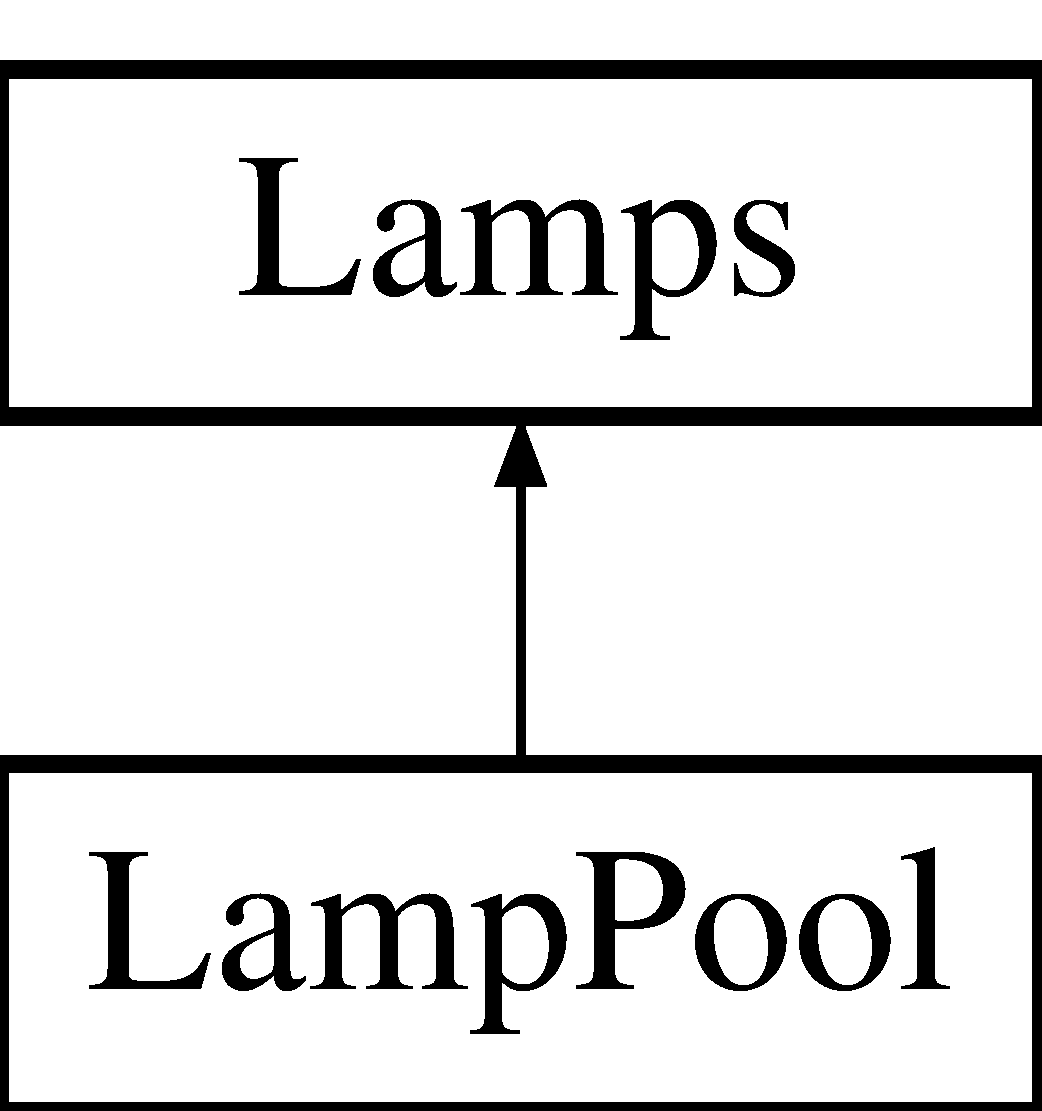
\includegraphics[height=2.000000cm]{classLampPool}
\end{center}
\end{figure}
\subsubsection*{\-Public \-Member \-Functions}
\begin{DoxyCompactItemize}
\item 
\hyperlink{classLampPool_a59801053a3a17434d2575c65dca4002f}{\-Lamp\-Pool} ()
\item 
\hyperlink{classLampPool_ab7ebd17476e0e4405ea2840d37506096}{$\sim$\-Lamp\-Pool} ()
\item 
int \hyperlink{classLampPool_a841fa821a574fce5706529ef342a7801}{get\-Num\-Lamps} ()
\item 
void \hyperlink{classLampPool_a1017c816b9d8690690812c83692cfe49}{set\-Value} (int, double)
\item 
double \hyperlink{classLampPool_acf6877e3883a9804ca1cefab5f6617da}{get\-Value} (int)
\item 
void \hyperlink{classLampPool_a6581aee51439dd08c8217d59a661afa3}{set\-All} (double)
\item 
bool \hyperlink{classLampPool_ab1ac3fbb0bf05504e21a84ed5856703e}{do\-Step} (double delta\-\_\-t)
\item 
void \hyperlink{classLampPool_a2b41e1640e50b736dafe8ceb69fe5bd5}{set\-Fade\-Speed} (double speed)
\item 
void \hyperlink{classLampPool_a0a904aa58951e12a3df7f39cb3c8f857}{set\-Update\-Rate} (double rate)
\item 
void \hyperlink{classLampPool_a93ec860020146d2d8e5779035b3a9b46}{start} ()
\item 
void \hyperlink{classLampPool_a0fd3756c9d927cc1d3dfec08228e1961}{stop} ()
\item 
bool \hyperlink{classLampPool_a6fff0dbb172914a107f4f99563306f49}{is\-Ready} ()
\item 
bool \hyperlink{classLampPool_a9df2536dce2e008da580c36ee69058c0}{send} ()
\item 
int \hyperlink{classLampPool_aec8bc100570e7eab3d59a3759ab0a164}{get\-Num\-Members} ()
\item 
\hyperlink{classLamps}{\-Lamps} $\ast$ \hyperlink{classLampPool_a38f0c6542e733a8e83c88176797e3130}{get\-Member} (int m)
\item 
void \hyperlink{classLampPool_aebf814163555551a356bcfa4730c5507}{add\-Member} (\hyperlink{classLamps}{\-Lamps} $\ast$lamps)
\end{DoxyCompactItemize}
\subsubsection*{\-Private \-Member \-Functions}
\begin{DoxyCompactItemize}
\item 
int \hyperlink{classLampPool_a74d1e9358bba1510873544f29e26ed2d}{get\-Member\-For\-Lamp\-Index} (int)
\item 
int \hyperlink{classLampPool_a63b0f102239f05edb6d8796568fa1bd4}{get\-Mapped\-Lamp\-Index} (int)
\end{DoxyCompactItemize}
\subsubsection*{\-Private \-Attributes}
\begin{DoxyCompactItemize}
\item 
vector$<$ \hyperlink{classLamps}{\-Lamps} $\ast$ $>$ \hyperlink{classLampPool_ad977e821c729cc6e55e56e462eea5596}{members}
\end{DoxyCompactItemize}


\subsubsection{\-Detailed \-Description}
\-Groups instances of \hyperlink{classLamps}{\-Lamps}. 

\subsubsection{\-Constructor \& \-Destructor \-Documentation}
\hypertarget{classLampPool_a59801053a3a17434d2575c65dca4002f}{\index{\-Lamp\-Pool@{\-Lamp\-Pool}!\-Lamp\-Pool@{\-Lamp\-Pool}}
\index{\-Lamp\-Pool@{\-Lamp\-Pool}!LampPool@{\-Lamp\-Pool}}
\paragraph[{\-Lamp\-Pool}]{\setlength{\rightskip}{0pt plus 5cm}{\bf \-Lamp\-Pool\-::\-Lamp\-Pool} (
\begin{DoxyParamCaption}
{}
\end{DoxyParamCaption}
)}}\label{classLampPool_a59801053a3a17434d2575c65dca4002f}
\begin{DoxyAuthor}{\-Author}
\-Manuel \-Jerger $<$\href{mailto:nom@nomnom.de}{\tt nom@nomnom.\-de}$>$
\end{DoxyAuthor}
\-This class represents a pool of lamps. \-It controls multiple \hyperlink{classLamps}{\-Lamps} classes and behaves like a single lamp class. \hypertarget{classLampPool_ab7ebd17476e0e4405ea2840d37506096}{\index{\-Lamp\-Pool@{\-Lamp\-Pool}!$\sim$\-Lamp\-Pool@{$\sim$\-Lamp\-Pool}}
\index{$\sim$\-Lamp\-Pool@{$\sim$\-Lamp\-Pool}!LampPool@{\-Lamp\-Pool}}
\paragraph[{$\sim$\-Lamp\-Pool}]{\setlength{\rightskip}{0pt plus 5cm}{\bf \-Lamp\-Pool\-::$\sim$\-Lamp\-Pool} (
\begin{DoxyParamCaption}
{}
\end{DoxyParamCaption}
)\hspace{0.3cm}{\ttfamily  \mbox{[}inline\mbox{]}}}}\label{classLampPool_ab7ebd17476e0e4405ea2840d37506096}


\subsubsection{\-Member \-Function \-Documentation}
\hypertarget{classLampPool_aebf814163555551a356bcfa4730c5507}{\index{\-Lamp\-Pool@{\-Lamp\-Pool}!add\-Member@{add\-Member}}
\index{add\-Member@{add\-Member}!LampPool@{\-Lamp\-Pool}}
\paragraph[{add\-Member}]{\setlength{\rightskip}{0pt plus 5cm}void {\bf \-Lamp\-Pool\-::add\-Member} (
\begin{DoxyParamCaption}
\item[{{\bf \-Lamps} $\ast$}]{lamps}
\end{DoxyParamCaption}
)}}\label{classLampPool_aebf814163555551a356bcfa4730c5507}
\hypertarget{classLampPool_ab1ac3fbb0bf05504e21a84ed5856703e}{\index{\-Lamp\-Pool@{\-Lamp\-Pool}!do\-Step@{do\-Step}}
\index{do\-Step@{do\-Step}!LampPool@{\-Lamp\-Pool}}
\paragraph[{do\-Step}]{\setlength{\rightskip}{0pt plus 5cm}bool {\bf \-Lamp\-Pool\-::do\-Step} (
\begin{DoxyParamCaption}
\item[{double}]{delta\-\_\-t}
\end{DoxyParamCaption}
)\hspace{0.3cm}{\ttfamily  \mbox{[}virtual\mbox{]}}}}\label{classLampPool_ab1ac3fbb0bf05504e21a84ed5856703e}
\-Does one fading step (if fadespeed $>$ 0) and calls \hyperlink{classLampPool_a9df2536dce2e008da580c36ee69058c0}{send()} at the end. 

\-Reimplemented from \hyperlink{classLamps_ad5805156c0984402c05df3256482b30c}{\-Lamps}.

\hypertarget{classLampPool_a63b0f102239f05edb6d8796568fa1bd4}{\index{\-Lamp\-Pool@{\-Lamp\-Pool}!get\-Mapped\-Lamp\-Index@{get\-Mapped\-Lamp\-Index}}
\index{get\-Mapped\-Lamp\-Index@{get\-Mapped\-Lamp\-Index}!LampPool@{\-Lamp\-Pool}}
\paragraph[{get\-Mapped\-Lamp\-Index}]{\setlength{\rightskip}{0pt plus 5cm}int {\bf \-Lamp\-Pool\-::get\-Mapped\-Lamp\-Index} (
\begin{DoxyParamCaption}
\item[{int}]{lamp\-I\-D}
\end{DoxyParamCaption}
)\hspace{0.3cm}{\ttfamily  \mbox{[}private\mbox{]}}}}\label{classLampPool_a63b0f102239f05edb6d8796568fa1bd4}
\hypertarget{classLampPool_a38f0c6542e733a8e83c88176797e3130}{\index{\-Lamp\-Pool@{\-Lamp\-Pool}!get\-Member@{get\-Member}}
\index{get\-Member@{get\-Member}!LampPool@{\-Lamp\-Pool}}
\paragraph[{get\-Member}]{\setlength{\rightskip}{0pt plus 5cm}{\bf \-Lamps} $\ast$ {\bf \-Lamp\-Pool\-::get\-Member} (
\begin{DoxyParamCaption}
\item[{int}]{m}
\end{DoxyParamCaption}
)}}\label{classLampPool_a38f0c6542e733a8e83c88176797e3130}
\hypertarget{classLampPool_a74d1e9358bba1510873544f29e26ed2d}{\index{\-Lamp\-Pool@{\-Lamp\-Pool}!get\-Member\-For\-Lamp\-Index@{get\-Member\-For\-Lamp\-Index}}
\index{get\-Member\-For\-Lamp\-Index@{get\-Member\-For\-Lamp\-Index}!LampPool@{\-Lamp\-Pool}}
\paragraph[{get\-Member\-For\-Lamp\-Index}]{\setlength{\rightskip}{0pt plus 5cm}int {\bf \-Lamp\-Pool\-::get\-Member\-For\-Lamp\-Index} (
\begin{DoxyParamCaption}
\item[{int}]{lamp\-I\-D}
\end{DoxyParamCaption}
)\hspace{0.3cm}{\ttfamily  \mbox{[}private\mbox{]}}}}\label{classLampPool_a74d1e9358bba1510873544f29e26ed2d}
\hypertarget{classLampPool_a841fa821a574fce5706529ef342a7801}{\index{\-Lamp\-Pool@{\-Lamp\-Pool}!get\-Num\-Lamps@{get\-Num\-Lamps}}
\index{get\-Num\-Lamps@{get\-Num\-Lamps}!LampPool@{\-Lamp\-Pool}}
\paragraph[{get\-Num\-Lamps}]{\setlength{\rightskip}{0pt plus 5cm}int {\bf \-Lamp\-Pool\-::get\-Num\-Lamps} (
\begin{DoxyParamCaption}
{}
\end{DoxyParamCaption}
)\hspace{0.3cm}{\ttfamily  \mbox{[}virtual\mbox{]}}}}\label{classLampPool_a841fa821a574fce5706529ef342a7801}


\-Reimplemented from \hyperlink{classLamps_a34fab22fb2de278133ef3ef2293e5597}{\-Lamps}.

\hypertarget{classLampPool_aec8bc100570e7eab3d59a3759ab0a164}{\index{\-Lamp\-Pool@{\-Lamp\-Pool}!get\-Num\-Members@{get\-Num\-Members}}
\index{get\-Num\-Members@{get\-Num\-Members}!LampPool@{\-Lamp\-Pool}}
\paragraph[{get\-Num\-Members}]{\setlength{\rightskip}{0pt plus 5cm}int {\bf \-Lamp\-Pool\-::get\-Num\-Members} (
\begin{DoxyParamCaption}
{}
\end{DoxyParamCaption}
)}}\label{classLampPool_aec8bc100570e7eab3d59a3759ab0a164}
\hypertarget{classLampPool_acf6877e3883a9804ca1cefab5f6617da}{\index{\-Lamp\-Pool@{\-Lamp\-Pool}!get\-Value@{get\-Value}}
\index{get\-Value@{get\-Value}!LampPool@{\-Lamp\-Pool}}
\paragraph[{get\-Value}]{\setlength{\rightskip}{0pt plus 5cm}double {\bf \-Lamp\-Pool\-::get\-Value} (
\begin{DoxyParamCaption}
\item[{int}]{lamp\-I\-D}
\end{DoxyParamCaption}
)\hspace{0.3cm}{\ttfamily  \mbox{[}virtual\mbox{]}}}}\label{classLampPool_acf6877e3883a9804ca1cefab5f6617da}
\-Return the current brightness of a single lamp. 

\-Reimplemented from \hyperlink{classLamps_a5759248dcf78231270ed88d3e24c83cc}{\-Lamps}.

\hypertarget{classLampPool_a6fff0dbb172914a107f4f99563306f49}{\index{\-Lamp\-Pool@{\-Lamp\-Pool}!is\-Ready@{is\-Ready}}
\index{is\-Ready@{is\-Ready}!LampPool@{\-Lamp\-Pool}}
\paragraph[{is\-Ready}]{\setlength{\rightskip}{0pt plus 5cm}bool {\bf \-Lamp\-Pool\-::is\-Ready} (
\begin{DoxyParamCaption}
{}
\end{DoxyParamCaption}
)\hspace{0.3cm}{\ttfamily  \mbox{[}virtual\mbox{]}}}}\label{classLampPool_a6fff0dbb172914a107f4f99563306f49}


\-Implements \hyperlink{classLamps_aad615bf90ffa5f5d52d409a354a1942a}{\-Lamps}.

\hypertarget{classLampPool_a9df2536dce2e008da580c36ee69058c0}{\index{\-Lamp\-Pool@{\-Lamp\-Pool}!send@{send}}
\index{send@{send}!LampPool@{\-Lamp\-Pool}}
\paragraph[{send}]{\setlength{\rightskip}{0pt plus 5cm}bool {\bf \-Lamp\-Pool\-::send} (
\begin{DoxyParamCaption}
{}
\end{DoxyParamCaption}
)\hspace{0.3cm}{\ttfamily  \mbox{[}virtual\mbox{]}}}}\label{classLampPool_a9df2536dce2e008da580c36ee69058c0}


\-Implements \hyperlink{classLamps_a9e5db6658a005b574d6344dab747bf4a}{\-Lamps}.

\hypertarget{classLampPool_a6581aee51439dd08c8217d59a661afa3}{\index{\-Lamp\-Pool@{\-Lamp\-Pool}!set\-All@{set\-All}}
\index{set\-All@{set\-All}!LampPool@{\-Lamp\-Pool}}
\paragraph[{set\-All}]{\setlength{\rightskip}{0pt plus 5cm}void {\bf \-Lamp\-Pool\-::set\-All} (
\begin{DoxyParamCaption}
\item[{double}]{brightness}
\end{DoxyParamCaption}
)\hspace{0.3cm}{\ttfamily  \mbox{[}virtual\mbox{]}}}}\label{classLampPool_a6581aee51439dd08c8217d59a661afa3}
\-Set all lamps to the specified brightness. 

\-Reimplemented from \hyperlink{classLamps_a658b32441ac2d59f61289e79fde12e3e}{\-Lamps}.

\hypertarget{classLampPool_a2b41e1640e50b736dafe8ceb69fe5bd5}{\index{\-Lamp\-Pool@{\-Lamp\-Pool}!set\-Fade\-Speed@{set\-Fade\-Speed}}
\index{set\-Fade\-Speed@{set\-Fade\-Speed}!LampPool@{\-Lamp\-Pool}}
\paragraph[{set\-Fade\-Speed}]{\setlength{\rightskip}{0pt plus 5cm}void {\bf \-Lamp\-Pool\-::set\-Fade\-Speed} (
\begin{DoxyParamCaption}
\item[{double}]{speed}
\end{DoxyParamCaption}
)\hspace{0.3cm}{\ttfamily  \mbox{[}virtual\mbox{]}}}}\label{classLampPool_a2b41e1640e50b736dafe8ceb69fe5bd5}


\-Reimplemented from \hyperlink{classLamps_a0d6ba649f7ca8883aaabc1dcc4e604c8}{\-Lamps}.

\hypertarget{classLampPool_a0a904aa58951e12a3df7f39cb3c8f857}{\index{\-Lamp\-Pool@{\-Lamp\-Pool}!set\-Update\-Rate@{set\-Update\-Rate}}
\index{set\-Update\-Rate@{set\-Update\-Rate}!LampPool@{\-Lamp\-Pool}}
\paragraph[{set\-Update\-Rate}]{\setlength{\rightskip}{0pt plus 5cm}void {\bf \-Lamp\-Pool\-::set\-Update\-Rate} (
\begin{DoxyParamCaption}
\item[{double}]{rate}
\end{DoxyParamCaption}
)\hspace{0.3cm}{\ttfamily  \mbox{[}virtual\mbox{]}}}}\label{classLampPool_a0a904aa58951e12a3df7f39cb3c8f857}


\-Reimplemented from \hyperlink{classLamps_a18cb9afa3dd13d877d8c48b1fc804a2d}{\-Lamps}.

\hypertarget{classLampPool_a1017c816b9d8690690812c83692cfe49}{\index{\-Lamp\-Pool@{\-Lamp\-Pool}!set\-Value@{set\-Value}}
\index{set\-Value@{set\-Value}!LampPool@{\-Lamp\-Pool}}
\paragraph[{set\-Value}]{\setlength{\rightskip}{0pt plus 5cm}void {\bf \-Lamp\-Pool\-::set\-Value} (
\begin{DoxyParamCaption}
\item[{int}]{lamp\-I\-D, }
\item[{double}]{brightness}
\end{DoxyParamCaption}
)\hspace{0.3cm}{\ttfamily  \mbox{[}virtual\mbox{]}}}}\label{classLampPool_a1017c816b9d8690690812c83692cfe49}
\-Sets the brightness of a lamp. \-If fading is enabled, it sets the target fade-\/to value. 

\-Reimplemented from \hyperlink{classLamps_a7d4b61ad0b436402fe57bd649f873ee2}{\-Lamps}.

\hypertarget{classLampPool_a93ec860020146d2d8e5779035b3a9b46}{\index{\-Lamp\-Pool@{\-Lamp\-Pool}!start@{start}}
\index{start@{start}!LampPool@{\-Lamp\-Pool}}
\paragraph[{start}]{\setlength{\rightskip}{0pt plus 5cm}void {\bf \-Lamp\-Pool\-::start} (
\begin{DoxyParamCaption}
{}
\end{DoxyParamCaption}
)}}\label{classLampPool_a93ec860020146d2d8e5779035b3a9b46}
\-Starts fading thread for automatic updating and fading. 

\-Reimplemented from \hyperlink{classLamps_a561aec75120eb6e76106659132a10632}{\-Lamps}.

\hypertarget{classLampPool_a0fd3756c9d927cc1d3dfec08228e1961}{\index{\-Lamp\-Pool@{\-Lamp\-Pool}!stop@{stop}}
\index{stop@{stop}!LampPool@{\-Lamp\-Pool}}
\paragraph[{stop}]{\setlength{\rightskip}{0pt plus 5cm}void {\bf \-Lamp\-Pool\-::stop} (
\begin{DoxyParamCaption}
{}
\end{DoxyParamCaption}
)}}\label{classLampPool_a0fd3756c9d927cc1d3dfec08228e1961}
\-Stops automatic updating. 

\-Reimplemented from \hyperlink{classLamps_adea5e864f8b721933e445b619bc5caec}{\-Lamps}.



\subsubsection{\-Field \-Documentation}
\hypertarget{classLampPool_ad977e821c729cc6e55e56e462eea5596}{\index{\-Lamp\-Pool@{\-Lamp\-Pool}!members@{members}}
\index{members@{members}!LampPool@{\-Lamp\-Pool}}
\paragraph[{members}]{\setlength{\rightskip}{0pt plus 5cm}vector$<${\bf \-Lamps}$\ast$$>$ {\bf \-Lamp\-Pool\-::members}\hspace{0.3cm}{\ttfamily  \mbox{[}private\mbox{]}}}}\label{classLampPool_ad977e821c729cc6e55e56e462eea5596}


\-The documentation for this class was generated from the following files\-:\begin{DoxyCompactItemize}
\item 
src/\hyperlink{lamppool_8h}{lamppool.\-h}\item 
src/\hyperlink{lamppool_8cpp}{lamppool.\-cpp}\end{DoxyCompactItemize}

\hypertarget{classLamps}{\subsection{\-Lamps \-Class \-Reference}
\label{classLamps}\index{\-Lamps@{\-Lamps}}
}


\-A monochrome lamp.  




{\ttfamily \#include $<$lamps.\-h$>$}

\-Inheritance diagram for \-Lamps\-:\begin{figure}[H]
\begin{center}
\leavevmode
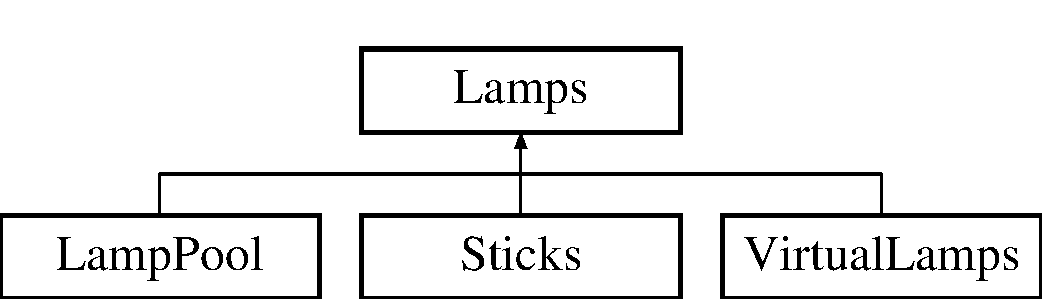
\includegraphics[height=2.000000cm]{classLamps}
\end{center}
\end{figure}
\subsubsection*{\-Public \-Member \-Functions}
\begin{DoxyCompactItemize}
\item 
\hyperlink{classLamps_a92824856cfa181b0632a17ab3a1129d2}{\-Lamps} ()
\item 
\hyperlink{classLamps_ac5d9774c29ce1712efcbb45152277181}{$\sim$\-Lamps} ()
\item 
virtual int \hyperlink{classLamps_a34fab22fb2de278133ef3ef2293e5597}{get\-Num\-Lamps} ()
\item 
virtual void \hyperlink{classLamps_a7d4b61ad0b436402fe57bd649f873ee2}{set\-Value} (int, double)
\item 
virtual double \hyperlink{classLamps_a5759248dcf78231270ed88d3e24c83cc}{get\-Value} (int)
\item 
virtual void \hyperlink{classLamps_a658b32441ac2d59f61289e79fde12e3e}{set\-All} (double)
\item 
void \hyperlink{classLamps_a561aec75120eb6e76106659132a10632}{start} ()
\item 
void \hyperlink{classLamps_adea5e864f8b721933e445b619bc5caec}{stop} ()
\item 
virtual bool \hyperlink{classLamps_ad5805156c0984402c05df3256482b30c}{do\-Step} (double delta\-\_\-t)
\item 
virtual void \hyperlink{classLamps_a0d6ba649f7ca8883aaabc1dcc4e604c8}{set\-Fade\-Speed} (double speed)
\item 
virtual void \hyperlink{classLamps_a18cb9afa3dd13d877d8c48b1fc804a2d}{set\-Update\-Rate} (double rate)
\item 
virtual bool \hyperlink{classLamps_aad615bf90ffa5f5d52d409a354a1942a}{is\-Ready} ()=0
\item 
virtual bool \hyperlink{classLamps_a9e5db6658a005b574d6344dab747bf4a}{send} ()=0
\end{DoxyCompactItemize}
\subsubsection*{\-Static \-Protected \-Member \-Functions}
\begin{DoxyCompactItemize}
\item 
static void $\ast$ \hyperlink{classLamps_ad6e04b6f320d75eacdcd45327bf8c80d}{start\-\_\-thread} (void $\ast$ptr)
\end{DoxyCompactItemize}
\subsubsection*{\-Protected \-Attributes}
\begin{DoxyCompactItemize}
\item 
bool \hyperlink{classLamps_a15b2fd60f5998f51d7b5e50e35c84329}{running}
\item 
int \hyperlink{classLamps_a64146e584dfa86281df86a37dd7cb772}{num\-Lamps}
\item 
vector$<$ double $>$ \hyperlink{classLamps_a12d0843f4f358ebd577089cb6c049076}{lamp\-Values}
\item 
vector$<$ double $>$ \hyperlink{classLamps_adc85fec25af923333458426f44504515}{previous\-Lamp\-Values}
\item 
vector$<$ double $>$ \hyperlink{classLamps_abf9da54471c9e73c99f955d75c7db949}{lamp\-Target\-Values}
\item 
double \hyperlink{classLamps_a77275168d36347133dec42259e88a1d4}{fade\-Speed}
\item 
double \hyperlink{classLamps_a31c7fbbc4d462b6b109f0c990e0e310f}{update\-Rate}
\end{DoxyCompactItemize}


\subsubsection{\-Detailed \-Description}
\-A monochrome lamp. 

\subsubsection{\-Constructor \& \-Destructor \-Documentation}
\hypertarget{classLamps_a92824856cfa181b0632a17ab3a1129d2}{\index{\-Lamps@{\-Lamps}!\-Lamps@{\-Lamps}}
\index{\-Lamps@{\-Lamps}!Lamps@{\-Lamps}}
\paragraph[{\-Lamps}]{\setlength{\rightskip}{0pt plus 5cm}{\bf \-Lamps\-::\-Lamps} (
\begin{DoxyParamCaption}
{}
\end{DoxyParamCaption}
)}}\label{classLamps_a92824856cfa181b0632a17ab3a1129d2}
\begin{DoxyAuthor}{\-Author}
\-Manuel \-Jerger $<$\href{mailto:nom@nomnom.de}{\tt nom@nomnom.\-de}$>$
\end{DoxyAuthor}
\-This abstract class represents a group of lamps of identical type (controlled by the same hardware). \-A lamp is monochrome and takes a rational value from 0..1 , where 1.\-0 is the maximum brightness and 0 turns the lamp off. \-It provides virtuals for setting lamp values, driving the hardware, automatic fading. \-It provides threaded updating. \hypertarget{classLamps_ac5d9774c29ce1712efcbb45152277181}{\index{\-Lamps@{\-Lamps}!$\sim$\-Lamps@{$\sim$\-Lamps}}
\index{$\sim$\-Lamps@{$\sim$\-Lamps}!Lamps@{\-Lamps}}
\paragraph[{$\sim$\-Lamps}]{\setlength{\rightskip}{0pt plus 5cm}{\bf \-Lamps\-::$\sim$\-Lamps} (
\begin{DoxyParamCaption}
{}
\end{DoxyParamCaption}
)}}\label{classLamps_ac5d9774c29ce1712efcbb45152277181}


\subsubsection{\-Member \-Function \-Documentation}
\hypertarget{classLamps_ad5805156c0984402c05df3256482b30c}{\index{\-Lamps@{\-Lamps}!do\-Step@{do\-Step}}
\index{do\-Step@{do\-Step}!Lamps@{\-Lamps}}
\paragraph[{do\-Step}]{\setlength{\rightskip}{0pt plus 5cm}bool {\bf \-Lamps\-::do\-Step} (
\begin{DoxyParamCaption}
\item[{double}]{delta\-\_\-t}
\end{DoxyParamCaption}
)\hspace{0.3cm}{\ttfamily  \mbox{[}virtual\mbox{]}}}}\label{classLamps_ad5805156c0984402c05df3256482b30c}
\-Does one fading step (if fadespeed $>$ 0) and calls \hyperlink{classLamps_a9e5db6658a005b574d6344dab747bf4a}{send()} at the end. 

\-Reimplemented in \hyperlink{classLampPool_ab1ac3fbb0bf05504e21a84ed5856703e}{\-Lamp\-Pool}.

\hypertarget{classLamps_a34fab22fb2de278133ef3ef2293e5597}{\index{\-Lamps@{\-Lamps}!get\-Num\-Lamps@{get\-Num\-Lamps}}
\index{get\-Num\-Lamps@{get\-Num\-Lamps}!Lamps@{\-Lamps}}
\paragraph[{get\-Num\-Lamps}]{\setlength{\rightskip}{0pt plus 5cm}int {\bf \-Lamps\-::get\-Num\-Lamps} (
\begin{DoxyParamCaption}
{}
\end{DoxyParamCaption}
)\hspace{0.3cm}{\ttfamily  \mbox{[}virtual\mbox{]}}}}\label{classLamps_a34fab22fb2de278133ef3ef2293e5597}


\-Reimplemented in \hyperlink{classLampPool_a841fa821a574fce5706529ef342a7801}{\-Lamp\-Pool}.

\hypertarget{classLamps_a5759248dcf78231270ed88d3e24c83cc}{\index{\-Lamps@{\-Lamps}!get\-Value@{get\-Value}}
\index{get\-Value@{get\-Value}!Lamps@{\-Lamps}}
\paragraph[{get\-Value}]{\setlength{\rightskip}{0pt plus 5cm}double {\bf \-Lamps\-::get\-Value} (
\begin{DoxyParamCaption}
\item[{int}]{lamp\-I\-D}
\end{DoxyParamCaption}
)\hspace{0.3cm}{\ttfamily  \mbox{[}virtual\mbox{]}}}}\label{classLamps_a5759248dcf78231270ed88d3e24c83cc}
\-Return the current brightness of a single lamp. 

\-Reimplemented in \hyperlink{classLampPool_acf6877e3883a9804ca1cefab5f6617da}{\-Lamp\-Pool}.

\hypertarget{classLamps_aad615bf90ffa5f5d52d409a354a1942a}{\index{\-Lamps@{\-Lamps}!is\-Ready@{is\-Ready}}
\index{is\-Ready@{is\-Ready}!Lamps@{\-Lamps}}
\paragraph[{is\-Ready}]{\setlength{\rightskip}{0pt plus 5cm}virtual bool {\bf \-Lamps\-::is\-Ready} (
\begin{DoxyParamCaption}
{}
\end{DoxyParamCaption}
)\hspace{0.3cm}{\ttfamily  \mbox{[}pure virtual\mbox{]}}}}\label{classLamps_aad615bf90ffa5f5d52d409a354a1942a}


\-Implemented in \hyperlink{classSticks_a6fc1fb933fbe6ce05ba88ef83322a0f1}{\-Sticks}, \hyperlink{classLampPool_a6fff0dbb172914a107f4f99563306f49}{\-Lamp\-Pool}, and \hyperlink{classVirtualLamps_ad1e55b2045b9bf34bc085fc79f47ef90}{\-Virtual\-Lamps}.

\hypertarget{classLamps_a9e5db6658a005b574d6344dab747bf4a}{\index{\-Lamps@{\-Lamps}!send@{send}}
\index{send@{send}!Lamps@{\-Lamps}}
\paragraph[{send}]{\setlength{\rightskip}{0pt plus 5cm}virtual bool {\bf \-Lamps\-::send} (
\begin{DoxyParamCaption}
{}
\end{DoxyParamCaption}
)\hspace{0.3cm}{\ttfamily  \mbox{[}pure virtual\mbox{]}}}}\label{classLamps_a9e5db6658a005b574d6344dab747bf4a}


\-Implemented in \hyperlink{classSticks_aa19dfda62c22c44cd4bda1e3abe3f0af}{\-Sticks}, \hyperlink{classLampPool_a9df2536dce2e008da580c36ee69058c0}{\-Lamp\-Pool}, and \hyperlink{classVirtualLamps_a0b1e1847c16c5283ad95c29f9142bbc9}{\-Virtual\-Lamps}.

\hypertarget{classLamps_a658b32441ac2d59f61289e79fde12e3e}{\index{\-Lamps@{\-Lamps}!set\-All@{set\-All}}
\index{set\-All@{set\-All}!Lamps@{\-Lamps}}
\paragraph[{set\-All}]{\setlength{\rightskip}{0pt plus 5cm}void {\bf \-Lamps\-::set\-All} (
\begin{DoxyParamCaption}
\item[{double}]{brightness}
\end{DoxyParamCaption}
)\hspace{0.3cm}{\ttfamily  \mbox{[}virtual\mbox{]}}}}\label{classLamps_a658b32441ac2d59f61289e79fde12e3e}
\-Set all lamps to the specified brightness. 

\-Reimplemented in \hyperlink{classLampPool_a6581aee51439dd08c8217d59a661afa3}{\-Lamp\-Pool}.

\hypertarget{classLamps_a0d6ba649f7ca8883aaabc1dcc4e604c8}{\index{\-Lamps@{\-Lamps}!set\-Fade\-Speed@{set\-Fade\-Speed}}
\index{set\-Fade\-Speed@{set\-Fade\-Speed}!Lamps@{\-Lamps}}
\paragraph[{set\-Fade\-Speed}]{\setlength{\rightskip}{0pt plus 5cm}void {\bf \-Lamps\-::set\-Fade\-Speed} (
\begin{DoxyParamCaption}
\item[{double}]{speed}
\end{DoxyParamCaption}
)\hspace{0.3cm}{\ttfamily  \mbox{[}virtual\mbox{]}}}}\label{classLamps_a0d6ba649f7ca8883aaabc1dcc4e604c8}


\-Reimplemented in \hyperlink{classLampPool_a2b41e1640e50b736dafe8ceb69fe5bd5}{\-Lamp\-Pool}.

\hypertarget{classLamps_a18cb9afa3dd13d877d8c48b1fc804a2d}{\index{\-Lamps@{\-Lamps}!set\-Update\-Rate@{set\-Update\-Rate}}
\index{set\-Update\-Rate@{set\-Update\-Rate}!Lamps@{\-Lamps}}
\paragraph[{set\-Update\-Rate}]{\setlength{\rightskip}{0pt plus 5cm}void {\bf \-Lamps\-::set\-Update\-Rate} (
\begin{DoxyParamCaption}
\item[{double}]{rate}
\end{DoxyParamCaption}
)\hspace{0.3cm}{\ttfamily  \mbox{[}virtual\mbox{]}}}}\label{classLamps_a18cb9afa3dd13d877d8c48b1fc804a2d}


\-Reimplemented in \hyperlink{classLampPool_a0a904aa58951e12a3df7f39cb3c8f857}{\-Lamp\-Pool}.

\hypertarget{classLamps_a7d4b61ad0b436402fe57bd649f873ee2}{\index{\-Lamps@{\-Lamps}!set\-Value@{set\-Value}}
\index{set\-Value@{set\-Value}!Lamps@{\-Lamps}}
\paragraph[{set\-Value}]{\setlength{\rightskip}{0pt plus 5cm}void {\bf \-Lamps\-::set\-Value} (
\begin{DoxyParamCaption}
\item[{int}]{lamp\-I\-D, }
\item[{double}]{brightness}
\end{DoxyParamCaption}
)\hspace{0.3cm}{\ttfamily  \mbox{[}virtual\mbox{]}}}}\label{classLamps_a7d4b61ad0b436402fe57bd649f873ee2}
\-Sets the brightness of a lamp. \-If fading is enabled, it sets the target fade-\/to value. 

\-Reimplemented in \hyperlink{classLampPool_a1017c816b9d8690690812c83692cfe49}{\-Lamp\-Pool}.

\hypertarget{classLamps_a561aec75120eb6e76106659132a10632}{\index{\-Lamps@{\-Lamps}!start@{start}}
\index{start@{start}!Lamps@{\-Lamps}}
\paragraph[{start}]{\setlength{\rightskip}{0pt plus 5cm}void {\bf \-Lamps\-::start} (
\begin{DoxyParamCaption}
{}
\end{DoxyParamCaption}
)}}\label{classLamps_a561aec75120eb6e76106659132a10632}
\-Starts fading thread for automatic updating and fading. 

\-Reimplemented in \hyperlink{classLampPool_a93ec860020146d2d8e5779035b3a9b46}{\-Lamp\-Pool}.

\hypertarget{classLamps_ad6e04b6f320d75eacdcd45327bf8c80d}{\index{\-Lamps@{\-Lamps}!start\-\_\-thread@{start\-\_\-thread}}
\index{start\-\_\-thread@{start\-\_\-thread}!Lamps@{\-Lamps}}
\paragraph[{start\-\_\-thread}]{\setlength{\rightskip}{0pt plus 5cm}void $\ast$ {\bf \-Lamps\-::start\-\_\-thread} (
\begin{DoxyParamCaption}
\item[{void $\ast$}]{ptr}
\end{DoxyParamCaption}
)\hspace{0.3cm}{\ttfamily  \mbox{[}static, protected\mbox{]}}}}\label{classLamps_ad6e04b6f320d75eacdcd45327bf8c80d}
\-The updating thread. \hypertarget{classLamps_adea5e864f8b721933e445b619bc5caec}{\index{\-Lamps@{\-Lamps}!stop@{stop}}
\index{stop@{stop}!Lamps@{\-Lamps}}
\paragraph[{stop}]{\setlength{\rightskip}{0pt plus 5cm}void {\bf \-Lamps\-::stop} (
\begin{DoxyParamCaption}
{}
\end{DoxyParamCaption}
)}}\label{classLamps_adea5e864f8b721933e445b619bc5caec}
\-Stops automatic updating. 

\-Reimplemented in \hyperlink{classLampPool_a0fd3756c9d927cc1d3dfec08228e1961}{\-Lamp\-Pool}.



\subsubsection{\-Field \-Documentation}
\hypertarget{classLamps_a77275168d36347133dec42259e88a1d4}{\index{\-Lamps@{\-Lamps}!fade\-Speed@{fade\-Speed}}
\index{fade\-Speed@{fade\-Speed}!Lamps@{\-Lamps}}
\paragraph[{fade\-Speed}]{\setlength{\rightskip}{0pt plus 5cm}double {\bf \-Lamps\-::fade\-Speed}\hspace{0.3cm}{\ttfamily  \mbox{[}protected\mbox{]}}}}\label{classLamps_a77275168d36347133dec42259e88a1d4}
\hypertarget{classLamps_abf9da54471c9e73c99f955d75c7db949}{\index{\-Lamps@{\-Lamps}!lamp\-Target\-Values@{lamp\-Target\-Values}}
\index{lamp\-Target\-Values@{lamp\-Target\-Values}!Lamps@{\-Lamps}}
\paragraph[{lamp\-Target\-Values}]{\setlength{\rightskip}{0pt plus 5cm}vector$<$double$>$ {\bf \-Lamps\-::lamp\-Target\-Values}\hspace{0.3cm}{\ttfamily  \mbox{[}protected\mbox{]}}}}\label{classLamps_abf9da54471c9e73c99f955d75c7db949}
\hypertarget{classLamps_a12d0843f4f358ebd577089cb6c049076}{\index{\-Lamps@{\-Lamps}!lamp\-Values@{lamp\-Values}}
\index{lamp\-Values@{lamp\-Values}!Lamps@{\-Lamps}}
\paragraph[{lamp\-Values}]{\setlength{\rightskip}{0pt plus 5cm}vector$<$double$>$ {\bf \-Lamps\-::lamp\-Values}\hspace{0.3cm}{\ttfamily  \mbox{[}protected\mbox{]}}}}\label{classLamps_a12d0843f4f358ebd577089cb6c049076}
\hypertarget{classLamps_a64146e584dfa86281df86a37dd7cb772}{\index{\-Lamps@{\-Lamps}!num\-Lamps@{num\-Lamps}}
\index{num\-Lamps@{num\-Lamps}!Lamps@{\-Lamps}}
\paragraph[{num\-Lamps}]{\setlength{\rightskip}{0pt plus 5cm}int {\bf \-Lamps\-::num\-Lamps}\hspace{0.3cm}{\ttfamily  \mbox{[}protected\mbox{]}}}}\label{classLamps_a64146e584dfa86281df86a37dd7cb772}
\hypertarget{classLamps_adc85fec25af923333458426f44504515}{\index{\-Lamps@{\-Lamps}!previous\-Lamp\-Values@{previous\-Lamp\-Values}}
\index{previous\-Lamp\-Values@{previous\-Lamp\-Values}!Lamps@{\-Lamps}}
\paragraph[{previous\-Lamp\-Values}]{\setlength{\rightskip}{0pt plus 5cm}vector$<$double$>$ {\bf \-Lamps\-::previous\-Lamp\-Values}\hspace{0.3cm}{\ttfamily  \mbox{[}protected\mbox{]}}}}\label{classLamps_adc85fec25af923333458426f44504515}
\hypertarget{classLamps_a15b2fd60f5998f51d7b5e50e35c84329}{\index{\-Lamps@{\-Lamps}!running@{running}}
\index{running@{running}!Lamps@{\-Lamps}}
\paragraph[{running}]{\setlength{\rightskip}{0pt plus 5cm}bool {\bf \-Lamps\-::running}\hspace{0.3cm}{\ttfamily  \mbox{[}protected\mbox{]}}}}\label{classLamps_a15b2fd60f5998f51d7b5e50e35c84329}
\hypertarget{classLamps_a31c7fbbc4d462b6b109f0c990e0e310f}{\index{\-Lamps@{\-Lamps}!update\-Rate@{update\-Rate}}
\index{update\-Rate@{update\-Rate}!Lamps@{\-Lamps}}
\paragraph[{update\-Rate}]{\setlength{\rightskip}{0pt plus 5cm}double {\bf \-Lamps\-::update\-Rate}\hspace{0.3cm}{\ttfamily  \mbox{[}protected\mbox{]}}}}\label{classLamps_a31c7fbbc4d462b6b109f0c990e0e310f}


\-The documentation for this class was generated from the following files\-:\begin{DoxyCompactItemize}
\item 
src/\hyperlink{lamps_8h}{lamps.\-h}\item 
src/\hyperlink{lamps_8cpp}{lamps.\-cpp}\end{DoxyCompactItemize}

\hypertarget{classLightprobe}{\subsection{\-Lightprobe \-Class \-Reference}
\label{classLightprobe}\index{\-Lightprobe@{\-Lightprobe}}
}


\-Our light probe model.  




{\ttfamily \#include $<$lightprobe.\-h$>$}

\subsubsection*{\-Data \-Structures}
\begin{DoxyCompactItemize}
\item 
struct \hyperlink{structLightprobe_1_1params}{params}
\begin{DoxyCompactList}\small\item\em \-Configuration of the light probe. \end{DoxyCompactList}\item 
struct \hyperlink{structLightprobe_1_1samplingParams}{sampling\-Params}
\begin{DoxyCompactList}\small\item\em \-Configures sampling. \end{DoxyCompactList}\end{DoxyCompactItemize}
\subsubsection*{\-Public \-Member \-Functions}
\begin{DoxyCompactItemize}
\item 
\hyperlink{classLightprobe_af35628975adf15e7baa3276bc07dee67}{\-Lightprobe} (\hyperlink{classSource}{\-Source} $\ast$, \hyperlink{structLightprobe_1_1params}{params} c, \hyperlink{structLightprobe_1_1samplingParams}{sampling\-Params} sampling)
\item 
\hyperlink{classLightprobe_a79eaa4f155d473b11d0d8542dd19b9ea}{\-Lightprobe} (\hyperlink{classSource}{\-Source} $\ast$, string config\-File, \hyperlink{structLightprobe_1_1samplingParams}{sampling\-Params} sampling)
\item 
\hyperlink{classLightprobe_af7fb7a3f8c3b27f6c79452a27689a2ce}{\-Lightprobe} (\hyperlink{classSource}{\-Source} $\ast$, \hyperlink{structLightprobe_1_1params}{params} c, \hyperlink{structLightprobe_1_1samplingParams}{sampling\-Params} sampling, \hyperlink{utils_8h_aac426d8086789d4d7e318436071c9754}{directions} \hyperlink{classLightprobe_ad3aa93672a623bfb704576c466a7769e}{sampling\-Dirs})
\item 
\hyperlink{classLightprobe_ae9b07c8d066a0e11fd507abbea58c9f1}{$\sim$\-Lightprobe} ()
\item 
\hyperlink{structLightprobe_1_1params}{params} \hyperlink{classLightprobe_aeae57bb50a4a34a0b4493edc7105aa14}{get\-Config} ()
\item 
\hyperlink{structLightprobe_1_1samplingParams}{sampling\-Params} \hyperlink{classLightprobe_af3318a51889cd0eb6be10db8a687e35a}{get\-Sampling\-Config} ()
\item 
\hyperlink{classSource}{\-Source} $\ast$ \hyperlink{classLightprobe_a51a1d2400e449cf562711edfb156a007}{get\-Source} ()
\item 
void \hyperlink{classLightprobe_ad0b80ec6a606302dbe8824531efe51ea}{acquire} ()
\item 
imglib\-::\-Image$<$ float $>$ \& \hyperlink{classLightprobe_ad088c4138632e186fadf2113877f3ee7}{get\-Image} ()
\item 
bool \hyperlink{classLightprobe_a3a02a401ef6e2128facb9402778b21e8}{has\-New\-Data} ()
\item 
void \hyperlink{classLightprobe_a54bc0e1006b77cd3dd13b1683a6ada5c}{set\-Rotation\-Y} (double rad)
\item 
void \hyperlink{classLightprobe_ae5622bdea250c1257a798c0f3a3928f5}{precalculate\-Direction\-Pixel\-Data} ()
\item 
void \hyperlink{classLightprobe_a912f27392e9da6a585e164a5d0666db2}{precalculate\-Sampling\-Directions} ()
\item 
void \hyperlink{classLightprobe_a39ea15d783af5027e86fbbfcbb58c64f}{precalculate\-Sampling\-Structure} ()
\item 
void \hyperlink{classLightprobe_a9d52017afe1d496f4ec4d7f30c080e6c}{precalculate\-Sampling\-Cones} ()
\item 
void \hyperlink{classLightprobe_aeb2723f1e8a00106f4c6b1f43fe52e2a}{precalculate\-Sampling\-Nearest\-Neighbors} ()
\item 
void \hyperlink{classLightprobe_a57d6dca11f80a9c901bf4a43e19c3fc0}{precalculate\-Sampling\-All\-Pixels} ()
\item 
vector$<$ \hyperlink{structrgb}{rgb} $>$ \hyperlink{classLightprobe_aaeb0935fae39511dce1701534eb2b3bd}{get\-Impact} ()
\item 
vector$<$ \hyperlink{structrgb}{rgb} $>$ \hyperlink{classLightprobe_a173c0c970cc98f140f64ada3b50aec35}{get\-Impact} (imglib\-::\-Image$<$ float $>$ \&img)
\item 
\-Vector3d \hyperlink{classLightprobe_adb355d76902749ca80366548c58de258}{get\-Direction\-From\-Pixel} (\-Vector2i pos)
\item 
\-Vector3d \hyperlink{classLightprobe_a67cef2ec8ecd3b915901e8ae6735f52b}{get\-Direction\-From\-Pixel\-Debevec} (\-Vector2i pos)
\end{DoxyCompactItemize}
\subsubsection*{\-Data \-Fields}
\begin{DoxyCompactItemize}
\item 
vector$<$ \-Vector2i $>$ \hyperlink{classLightprobe_a47e0a0ac6509b630c45b26ea50c3bc6a}{all\-Pixels}
\item 
\hyperlink{utils_8h_aac426d8086789d4d7e318436071c9754}{directions} \hyperlink{classLightprobe_a95e255a27e98a2c0b2d4df167365ccdd}{all\-Dirs}
\item 
\hyperlink{utils_8h_aac426d8086789d4d7e318436071c9754}{directions} \hyperlink{classLightprobe_ad3aa93672a623bfb704576c466a7769e}{sampling\-Dirs}
\item 
vector$<$ \hyperlink{structdirCone}{dir\-Cone} $>$ \hyperlink{classLightprobe_a3bf62d3debaba3f19e2587d9e22ce204}{sampling\-Cones}
\item 
vector$<$ bool $>$ \hyperlink{classLightprobe_a9f5c4447d145b52e5fe27d8bd6cdcfca}{used\-Directions}
\end{DoxyCompactItemize}
\subsubsection*{\-Private \-Member \-Functions}
\begin{DoxyCompactItemize}
\item 
void \hyperlink{classLightprobe_a7e2724a719ccd14779aaeb7225b0acc3}{init} ()
\end{DoxyCompactItemize}
\subsubsection*{\-Private \-Attributes}
\begin{DoxyCompactItemize}
\item 
\hyperlink{structLightprobe_1_1params}{params} \hyperlink{classLightprobe_a2a75a5ac0b6fd74f9b6007e6f4bee079}{config}
\item 
\hyperlink{structLightprobe_1_1samplingParams}{sampling\-Params} \hyperlink{classLightprobe_a8b0f2510b3c39b154ef72d571f46c16b}{sampling\-Config}
\item 
\hyperlink{classSource}{\-Source} $\ast$ \hyperlink{classLightprobe_af923276096b3466a64bdda7bd76ed036}{source}
\item 
imglib\-::\-Image$<$ float $>$ \hyperlink{classLightprobe_aab72db6ab7c231959a7c5943ca8fc97f}{mask\-Image}
\item 
double \hyperlink{classLightprobe_a44b795e2f349dd13489799890bd86c9a}{plane\-Shift}
\end{DoxyCompactItemize}


\subsubsection{\-Detailed \-Description}
\-Our light probe model. 

\subsubsection{\-Constructor \& \-Destructor \-Documentation}
\hypertarget{classLightprobe_af35628975adf15e7baa3276bc07dee67}{\index{\-Lightprobe@{\-Lightprobe}!\-Lightprobe@{\-Lightprobe}}
\index{\-Lightprobe@{\-Lightprobe}!Lightprobe@{\-Lightprobe}}
\paragraph[{\-Lightprobe}]{\setlength{\rightskip}{0pt plus 5cm}{\bf \-Lightprobe\-::\-Lightprobe} (
\begin{DoxyParamCaption}
\item[{{\bf \-Source} $\ast$}]{s, }
\item[{{\bf params}}]{c, }
\item[{{\bf sampling\-Params}}]{sampling}
\end{DoxyParamCaption}
)}}\label{classLightprobe_af35628975adf15e7baa3276bc07dee67}
\-Set up light probe model from a given model config and sampling config. \hypertarget{classLightprobe_a79eaa4f155d473b11d0d8542dd19b9ea}{\index{\-Lightprobe@{\-Lightprobe}!\-Lightprobe@{\-Lightprobe}}
\index{\-Lightprobe@{\-Lightprobe}!Lightprobe@{\-Lightprobe}}
\paragraph[{\-Lightprobe}]{\setlength{\rightskip}{0pt plus 5cm}{\bf \-Lightprobe\-::\-Lightprobe} (
\begin{DoxyParamCaption}
\item[{{\bf \-Source} $\ast$}]{s, }
\item[{string}]{config\-File, }
\item[{{\bf sampling\-Params}}]{sampling}
\end{DoxyParamCaption}
)}}\label{classLightprobe_a79eaa4f155d473b11d0d8542dd19b9ea}
\-Set up light probe model using a given sampling configuration. \-Loads model config from file. \hypertarget{classLightprobe_af7fb7a3f8c3b27f6c79452a27689a2ce}{\index{\-Lightprobe@{\-Lightprobe}!\-Lightprobe@{\-Lightprobe}}
\index{\-Lightprobe@{\-Lightprobe}!Lightprobe@{\-Lightprobe}}
\paragraph[{\-Lightprobe}]{\setlength{\rightskip}{0pt plus 5cm}{\bf \-Lightprobe\-::\-Lightprobe} (
\begin{DoxyParamCaption}
\item[{{\bf \-Source} $\ast$}]{s, }
\item[{{\bf params}}]{c, }
\item[{{\bf sampling\-Params}}]{sampling, }
\item[{{\bf directions}}]{sampling\-Dirs}
\end{DoxyParamCaption}
)}}\label{classLightprobe_af7fb7a3f8c3b27f6c79452a27689a2ce}
\-Set up light probe model using a given sampling configuration and sampling directions. \-Loads model config from file. \hypertarget{classLightprobe_ae9b07c8d066a0e11fd507abbea58c9f1}{\index{\-Lightprobe@{\-Lightprobe}!$\sim$\-Lightprobe@{$\sim$\-Lightprobe}}
\index{$\sim$\-Lightprobe@{$\sim$\-Lightprobe}!Lightprobe@{\-Lightprobe}}
\paragraph[{$\sim$\-Lightprobe}]{\setlength{\rightskip}{0pt plus 5cm}{\bf \-Lightprobe\-::$\sim$\-Lightprobe} (
\begin{DoxyParamCaption}
{}
\end{DoxyParamCaption}
)}}\label{classLightprobe_ae9b07c8d066a0e11fd507abbea58c9f1}


\subsubsection{\-Member \-Function \-Documentation}
\hypertarget{classLightprobe_ad0b80ec6a606302dbe8824531efe51ea}{\index{\-Lightprobe@{\-Lightprobe}!acquire@{acquire}}
\index{acquire@{acquire}!Lightprobe@{\-Lightprobe}}
\paragraph[{acquire}]{\setlength{\rightskip}{0pt plus 5cm}void {\bf \-Lightprobe\-::acquire} (
\begin{DoxyParamCaption}
{}
\end{DoxyParamCaption}
)}}\label{classLightprobe_ad0b80ec6a606302dbe8824531efe51ea}
\hypertarget{classLightprobe_aeae57bb50a4a34a0b4493edc7105aa14}{\index{\-Lightprobe@{\-Lightprobe}!get\-Config@{get\-Config}}
\index{get\-Config@{get\-Config}!Lightprobe@{\-Lightprobe}}
\paragraph[{get\-Config}]{\setlength{\rightskip}{0pt plus 5cm}{\bf \-Lightprobe\-::params} {\bf \-Lightprobe\-::get\-Config} (
\begin{DoxyParamCaption}
{}
\end{DoxyParamCaption}
)}}\label{classLightprobe_aeae57bb50a4a34a0b4493edc7105aa14}
\hypertarget{classLightprobe_adb355d76902749ca80366548c58de258}{\index{\-Lightprobe@{\-Lightprobe}!get\-Direction\-From\-Pixel@{get\-Direction\-From\-Pixel}}
\index{get\-Direction\-From\-Pixel@{get\-Direction\-From\-Pixel}!Lightprobe@{\-Lightprobe}}
\paragraph[{get\-Direction\-From\-Pixel}]{\setlength{\rightskip}{0pt plus 5cm}\-Vector3d {\bf \-Lightprobe\-::get\-Direction\-From\-Pixel} (
\begin{DoxyParamCaption}
\item[{\-Vector2i}]{pos}
\end{DoxyParamCaption}
)}}\label{classLightprobe_adb355d76902749ca80366548c58de258}
\-Our light probe model. \-Calculates the reflected light direction from pixel coordinates. \hypertarget{classLightprobe_a67cef2ec8ecd3b915901e8ae6735f52b}{\index{\-Lightprobe@{\-Lightprobe}!get\-Direction\-From\-Pixel\-Debevec@{get\-Direction\-From\-Pixel\-Debevec}}
\index{get\-Direction\-From\-Pixel\-Debevec@{get\-Direction\-From\-Pixel\-Debevec}!Lightprobe@{\-Lightprobe}}
\paragraph[{get\-Direction\-From\-Pixel\-Debevec}]{\setlength{\rightskip}{0pt plus 5cm}\-Vector3d {\bf \-Lightprobe\-::get\-Direction\-From\-Pixel\-Debevec} (
\begin{DoxyParamCaption}
\item[{\-Vector2i}]{pos}
\end{DoxyParamCaption}
)}}\label{classLightprobe_a67cef2ec8ecd3b915901e8ae6735f52b}
\-Light probe model that use the \-Debevec parametrisation. \hypertarget{classLightprobe_ad088c4138632e186fadf2113877f3ee7}{\index{\-Lightprobe@{\-Lightprobe}!get\-Image@{get\-Image}}
\index{get\-Image@{get\-Image}!Lightprobe@{\-Lightprobe}}
\paragraph[{get\-Image}]{\setlength{\rightskip}{0pt plus 5cm}imglib\-::\-Image$<$ float $>$ \& {\bf \-Lightprobe\-::get\-Image} (
\begin{DoxyParamCaption}
{}
\end{DoxyParamCaption}
)}}\label{classLightprobe_ad088c4138632e186fadf2113877f3ee7}
\hypertarget{classLightprobe_aaeb0935fae39511dce1701534eb2b3bd}{\index{\-Lightprobe@{\-Lightprobe}!get\-Impact@{get\-Impact}}
\index{get\-Impact@{get\-Impact}!Lightprobe@{\-Lightprobe}}
\paragraph[{get\-Impact}]{\setlength{\rightskip}{0pt plus 5cm}vector$<$ {\bf rgb} $>$ {\bf \-Lightprobe\-::get\-Impact} (
\begin{DoxyParamCaption}
{}
\end{DoxyParamCaption}
)}}\label{classLightprobe_aaeb0935fae39511dce1701534eb2b3bd}
\-Calculates the impact of a lamp\-: \-Acquires an image from the source, performs downsampling and returns the sampled values. \hypertarget{classLightprobe_a173c0c970cc98f140f64ada3b50aec35}{\index{\-Lightprobe@{\-Lightprobe}!get\-Impact@{get\-Impact}}
\index{get\-Impact@{get\-Impact}!Lightprobe@{\-Lightprobe}}
\paragraph[{get\-Impact}]{\setlength{\rightskip}{0pt plus 5cm}vector$<$ {\bf rgb} $>$ {\bf \-Lightprobe\-::get\-Impact} (
\begin{DoxyParamCaption}
\item[{imglib\-::\-Image$<$ float $>$ \&}]{img}
\end{DoxyParamCaption}
)}}\label{classLightprobe_a173c0c970cc98f140f64ada3b50aec35}
\-Samples a light probe image. \hypertarget{classLightprobe_af3318a51889cd0eb6be10db8a687e35a}{\index{\-Lightprobe@{\-Lightprobe}!get\-Sampling\-Config@{get\-Sampling\-Config}}
\index{get\-Sampling\-Config@{get\-Sampling\-Config}!Lightprobe@{\-Lightprobe}}
\paragraph[{get\-Sampling\-Config}]{\setlength{\rightskip}{0pt plus 5cm}{\bf \-Lightprobe\-::sampling\-Params} {\bf \-Lightprobe\-::get\-Sampling\-Config} (
\begin{DoxyParamCaption}
{}
\end{DoxyParamCaption}
)}}\label{classLightprobe_af3318a51889cd0eb6be10db8a687e35a}
\hypertarget{classLightprobe_a51a1d2400e449cf562711edfb156a007}{\index{\-Lightprobe@{\-Lightprobe}!get\-Source@{get\-Source}}
\index{get\-Source@{get\-Source}!Lightprobe@{\-Lightprobe}}
\paragraph[{get\-Source}]{\setlength{\rightskip}{0pt plus 5cm}{\bf \-Source} $\ast$ {\bf \-Lightprobe\-::get\-Source} (
\begin{DoxyParamCaption}
{}
\end{DoxyParamCaption}
)}}\label{classLightprobe_a51a1d2400e449cf562711edfb156a007}
\hypertarget{classLightprobe_a3a02a401ef6e2128facb9402778b21e8}{\index{\-Lightprobe@{\-Lightprobe}!has\-New\-Data@{has\-New\-Data}}
\index{has\-New\-Data@{has\-New\-Data}!Lightprobe@{\-Lightprobe}}
\paragraph[{has\-New\-Data}]{\setlength{\rightskip}{0pt plus 5cm}bool {\bf \-Lightprobe\-::has\-New\-Data} (
\begin{DoxyParamCaption}
{}
\end{DoxyParamCaption}
)}}\label{classLightprobe_a3a02a401ef6e2128facb9402778b21e8}
\hypertarget{classLightprobe_a7e2724a719ccd14779aaeb7225b0acc3}{\index{\-Lightprobe@{\-Lightprobe}!init@{init}}
\index{init@{init}!Lightprobe@{\-Lightprobe}}
\paragraph[{init}]{\setlength{\rightskip}{0pt plus 5cm}void {\bf \-Lightprobe\-::init} (
\begin{DoxyParamCaption}
{}
\end{DoxyParamCaption}
)\hspace{0.3cm}{\ttfamily  \mbox{[}private\mbox{]}}}}\label{classLightprobe_a7e2724a719ccd14779aaeb7225b0acc3}
\-Initializes the light probe model. \hypertarget{classLightprobe_ae5622bdea250c1257a798c0f3a3928f5}{\index{\-Lightprobe@{\-Lightprobe}!precalculate\-Direction\-Pixel\-Data@{precalculate\-Direction\-Pixel\-Data}}
\index{precalculate\-Direction\-Pixel\-Data@{precalculate\-Direction\-Pixel\-Data}!Lightprobe@{\-Lightprobe}}
\paragraph[{precalculate\-Direction\-Pixel\-Data}]{\setlength{\rightskip}{0pt plus 5cm}void {\bf \-Lightprobe\-::precalculate\-Direction\-Pixel\-Data} (
\begin{DoxyParamCaption}
{}
\end{DoxyParamCaption}
)}}\label{classLightprobe_ae5622bdea250c1257a798c0f3a3928f5}
\-Precalculates the direction of reflected light for all available, unmasked pixels within the sampling range. \hypertarget{classLightprobe_a57d6dca11f80a9c901bf4a43e19c3fc0}{\index{\-Lightprobe@{\-Lightprobe}!precalculate\-Sampling\-All\-Pixels@{precalculate\-Sampling\-All\-Pixels}}
\index{precalculate\-Sampling\-All\-Pixels@{precalculate\-Sampling\-All\-Pixels}!Lightprobe@{\-Lightprobe}}
\paragraph[{precalculate\-Sampling\-All\-Pixels}]{\setlength{\rightskip}{0pt plus 5cm}void {\bf \-Lightprobe\-::precalculate\-Sampling\-All\-Pixels} (
\begin{DoxyParamCaption}
{}
\end{DoxyParamCaption}
)}}\label{classLightprobe_a57d6dca11f80a9c901bf4a43e19c3fc0}
\-Generates sampling structure for all-\/pixel sampling (every pixel becomes one direction). \hypertarget{classLightprobe_a9d52017afe1d496f4ec4d7f30c080e6c}{\index{\-Lightprobe@{\-Lightprobe}!precalculate\-Sampling\-Cones@{precalculate\-Sampling\-Cones}}
\index{precalculate\-Sampling\-Cones@{precalculate\-Sampling\-Cones}!Lightprobe@{\-Lightprobe}}
\paragraph[{precalculate\-Sampling\-Cones}]{\setlength{\rightskip}{0pt plus 5cm}void {\bf \-Lightprobe\-::precalculate\-Sampling\-Cones} (
\begin{DoxyParamCaption}
{}
\end{DoxyParamCaption}
)}}\label{classLightprobe_a9d52017afe1d496f4ec4d7f30c080e6c}
\-Generate sampling data structure for \-Gaussian sampling. \hypertarget{classLightprobe_a912f27392e9da6a585e164a5d0666db2}{\index{\-Lightprobe@{\-Lightprobe}!precalculate\-Sampling\-Directions@{precalculate\-Sampling\-Directions}}
\index{precalculate\-Sampling\-Directions@{precalculate\-Sampling\-Directions}!Lightprobe@{\-Lightprobe}}
\paragraph[{precalculate\-Sampling\-Directions}]{\setlength{\rightskip}{0pt plus 5cm}void {\bf \-Lightprobe\-::precalculate\-Sampling\-Directions} (
\begin{DoxyParamCaption}
{}
\end{DoxyParamCaption}
)}}\label{classLightprobe_a912f27392e9da6a585e164a5d0666db2}
\-Precalculates the sampling directions. \hypertarget{classLightprobe_aeb2723f1e8a00106f4c6b1f43fe52e2a}{\index{\-Lightprobe@{\-Lightprobe}!precalculate\-Sampling\-Nearest\-Neighbors@{precalculate\-Sampling\-Nearest\-Neighbors}}
\index{precalculate\-Sampling\-Nearest\-Neighbors@{precalculate\-Sampling\-Nearest\-Neighbors}!Lightprobe@{\-Lightprobe}}
\paragraph[{precalculate\-Sampling\-Nearest\-Neighbors}]{\setlength{\rightskip}{0pt plus 5cm}void {\bf \-Lightprobe\-::precalculate\-Sampling\-Nearest\-Neighbors} (
\begin{DoxyParamCaption}
{}
\end{DoxyParamCaption}
)}}\label{classLightprobe_aeb2723f1e8a00106f4c6b1f43fe52e2a}
\-Generates sampling datastructure for nearest-\/neighbor sampling. \hypertarget{classLightprobe_a39ea15d783af5027e86fbbfcbb58c64f}{\index{\-Lightprobe@{\-Lightprobe}!precalculate\-Sampling\-Structure@{precalculate\-Sampling\-Structure}}
\index{precalculate\-Sampling\-Structure@{precalculate\-Sampling\-Structure}!Lightprobe@{\-Lightprobe}}
\paragraph[{precalculate\-Sampling\-Structure}]{\setlength{\rightskip}{0pt plus 5cm}void {\bf \-Lightprobe\-::precalculate\-Sampling\-Structure} (
\begin{DoxyParamCaption}
{}
\end{DoxyParamCaption}
)}}\label{classLightprobe_a39ea15d783af5027e86fbbfcbb58c64f}
\-Generates the sampling data structure. \hypertarget{classLightprobe_a54bc0e1006b77cd3dd13b1683a6ada5c}{\index{\-Lightprobe@{\-Lightprobe}!set\-Rotation\-Y@{set\-Rotation\-Y}}
\index{set\-Rotation\-Y@{set\-Rotation\-Y}!Lightprobe@{\-Lightprobe}}
\paragraph[{set\-Rotation\-Y}]{\setlength{\rightskip}{0pt plus 5cm}void {\bf \-Lightprobe\-::set\-Rotation\-Y} (
\begin{DoxyParamCaption}
\item[{double}]{rad}
\end{DoxyParamCaption}
)}}\label{classLightprobe_a54bc0e1006b77cd3dd13b1683a6ada5c}
\-Set new value for rotation around y axis (on planar plane) and recalculate sampling datastructures 

\subsubsection{\-Field \-Documentation}
\hypertarget{classLightprobe_a95e255a27e98a2c0b2d4df167365ccdd}{\index{\-Lightprobe@{\-Lightprobe}!all\-Dirs@{all\-Dirs}}
\index{all\-Dirs@{all\-Dirs}!Lightprobe@{\-Lightprobe}}
\paragraph[{all\-Dirs}]{\setlength{\rightskip}{0pt plus 5cm}{\bf directions} {\bf \-Lightprobe\-::all\-Dirs}}}\label{classLightprobe_a95e255a27e98a2c0b2d4df167365ccdd}
\hypertarget{classLightprobe_a47e0a0ac6509b630c45b26ea50c3bc6a}{\index{\-Lightprobe@{\-Lightprobe}!all\-Pixels@{all\-Pixels}}
\index{all\-Pixels@{all\-Pixels}!Lightprobe@{\-Lightprobe}}
\paragraph[{all\-Pixels}]{\setlength{\rightskip}{0pt plus 5cm}vector$<$\-Vector2i$>$ {\bf \-Lightprobe\-::all\-Pixels}}}\label{classLightprobe_a47e0a0ac6509b630c45b26ea50c3bc6a}
\hypertarget{classLightprobe_a2a75a5ac0b6fd74f9b6007e6f4bee079}{\index{\-Lightprobe@{\-Lightprobe}!config@{config}}
\index{config@{config}!Lightprobe@{\-Lightprobe}}
\paragraph[{config}]{\setlength{\rightskip}{0pt plus 5cm}{\bf params} {\bf \-Lightprobe\-::config}\hspace{0.3cm}{\ttfamily  \mbox{[}private\mbox{]}}}}\label{classLightprobe_a2a75a5ac0b6fd74f9b6007e6f4bee079}
\hypertarget{classLightprobe_aab72db6ab7c231959a7c5943ca8fc97f}{\index{\-Lightprobe@{\-Lightprobe}!mask\-Image@{mask\-Image}}
\index{mask\-Image@{mask\-Image}!Lightprobe@{\-Lightprobe}}
\paragraph[{mask\-Image}]{\setlength{\rightskip}{0pt plus 5cm}imglib\-::\-Image$<$float$>$ {\bf \-Lightprobe\-::mask\-Image}\hspace{0.3cm}{\ttfamily  \mbox{[}private\mbox{]}}}}\label{classLightprobe_aab72db6ab7c231959a7c5943ca8fc97f}
\hypertarget{classLightprobe_a44b795e2f349dd13489799890bd86c9a}{\index{\-Lightprobe@{\-Lightprobe}!plane\-Shift@{plane\-Shift}}
\index{plane\-Shift@{plane\-Shift}!Lightprobe@{\-Lightprobe}}
\paragraph[{plane\-Shift}]{\setlength{\rightskip}{0pt plus 5cm}double {\bf \-Lightprobe\-::plane\-Shift}\hspace{0.3cm}{\ttfamily  \mbox{[}private\mbox{]}}}}\label{classLightprobe_a44b795e2f349dd13489799890bd86c9a}
\hypertarget{classLightprobe_a3bf62d3debaba3f19e2587d9e22ce204}{\index{\-Lightprobe@{\-Lightprobe}!sampling\-Cones@{sampling\-Cones}}
\index{sampling\-Cones@{sampling\-Cones}!Lightprobe@{\-Lightprobe}}
\paragraph[{sampling\-Cones}]{\setlength{\rightskip}{0pt plus 5cm}vector$<${\bf dir\-Cone}$>$ {\bf \-Lightprobe\-::sampling\-Cones}}}\label{classLightprobe_a3bf62d3debaba3f19e2587d9e22ce204}
\hypertarget{classLightprobe_a8b0f2510b3c39b154ef72d571f46c16b}{\index{\-Lightprobe@{\-Lightprobe}!sampling\-Config@{sampling\-Config}}
\index{sampling\-Config@{sampling\-Config}!Lightprobe@{\-Lightprobe}}
\paragraph[{sampling\-Config}]{\setlength{\rightskip}{0pt plus 5cm}{\bf sampling\-Params} {\bf \-Lightprobe\-::sampling\-Config}\hspace{0.3cm}{\ttfamily  \mbox{[}private\mbox{]}}}}\label{classLightprobe_a8b0f2510b3c39b154ef72d571f46c16b}
\hypertarget{classLightprobe_ad3aa93672a623bfb704576c466a7769e}{\index{\-Lightprobe@{\-Lightprobe}!sampling\-Dirs@{sampling\-Dirs}}
\index{sampling\-Dirs@{sampling\-Dirs}!Lightprobe@{\-Lightprobe}}
\paragraph[{sampling\-Dirs}]{\setlength{\rightskip}{0pt plus 5cm}{\bf directions} {\bf \-Lightprobe\-::sampling\-Dirs}}}\label{classLightprobe_ad3aa93672a623bfb704576c466a7769e}
\hypertarget{classLightprobe_af923276096b3466a64bdda7bd76ed036}{\index{\-Lightprobe@{\-Lightprobe}!source@{source}}
\index{source@{source}!Lightprobe@{\-Lightprobe}}
\paragraph[{source}]{\setlength{\rightskip}{0pt plus 5cm}{\bf \-Source}$\ast$ {\bf \-Lightprobe\-::source}\hspace{0.3cm}{\ttfamily  \mbox{[}private\mbox{]}}}}\label{classLightprobe_af923276096b3466a64bdda7bd76ed036}
\hypertarget{classLightprobe_a9f5c4447d145b52e5fe27d8bd6cdcfca}{\index{\-Lightprobe@{\-Lightprobe}!used\-Directions@{used\-Directions}}
\index{used\-Directions@{used\-Directions}!Lightprobe@{\-Lightprobe}}
\paragraph[{used\-Directions}]{\setlength{\rightskip}{0pt plus 5cm}vector$<$bool$>$ {\bf \-Lightprobe\-::used\-Directions}}}\label{classLightprobe_a9f5c4447d145b52e5fe27d8bd6cdcfca}


\-The documentation for this class was generated from the following files\-:\begin{DoxyCompactItemize}
\item 
src/\hyperlink{lightprobe_8h}{lightprobe.\-h}\item 
src/\hyperlink{lightprobe_8cpp}{lightprobe.\-cpp}\end{DoxyCompactItemize}

\hypertarget{structLightprobe_1_1params}{\subsection{\-Lightprobe\-:\-:params \-Struct \-Reference}
\label{structLightprobe_1_1params}\index{\-Lightprobe\-::params@{\-Lightprobe\-::params}}
}


\-Configuration of the light probe.  




{\ttfamily \#include $<$lightprobe.\-h$>$}

\subsubsection*{\-Public \-Member \-Functions}
\begin{DoxyCompactItemize}
\item 
\hyperlink{structLightprobe_1_1params_a347fa0f6a9b39bffe67cd0ec7aef10fb}{params} ()
\item 
void \hyperlink{structLightprobe_1_1params_a53a42706621d09f9f8425e530e75a4bb}{load} (string file)
\item 
void \hyperlink{structLightprobe_1_1params_a66c374957c19b4e7dec7c4db52da6d50}{save} (string file)
\end{DoxyCompactItemize}
\subsubsection*{\-Data \-Fields}
\begin{DoxyCompactItemize}
\item 
double \hyperlink{structLightprobe_1_1params_a1a40e9d1a193fe336b474170c5533b64}{cam\-Distance}
\item 
double \hyperlink{structLightprobe_1_1params_ac8ab0a15e712949c6826b9e7f8a12b01}{sphere\-Radius}
\item 
\hyperlink{structcircle}{circle} \hyperlink{structLightprobe_1_1params_a44ffbf9ece76217468bffd79aab5cff1}{sphere\-Circle}
\item 
double \hyperlink{structLightprobe_1_1params_a188ea2369fb3f908e768cdcae93b11da}{gamma}
\item 
\hyperlink{structrgb}{rgb} \hyperlink{structLightprobe_1_1params_a70ece8306fa1403868ec00f9eb5a1127}{whitepoint}
\item 
double \hyperlink{structLightprobe_1_1params_ac2ffd114db0a34902f8b5ea685284418}{exposure}
\item 
\-Vector3d \hyperlink{structLightprobe_1_1params_a350177e1cf207849d610e05a9e1519f5}{rotation}
\item 
double \hyperlink{structLightprobe_1_1params_ac11dff747b25a1afbafa8a606b17adab}{horizon\-Angle}
\item 
string \hyperlink{structLightprobe_1_1params_a326b53e98cb82cc98b035563ea24a202}{response\-Curve}
\item 
string \hyperlink{structLightprobe_1_1params_aa43a9ea2e25549878c90b8be9d48fa4a}{mask\-File}
\item 
int \hyperlink{structLightprobe_1_1params_ab0c81bf7acce654fa389579d66cb4a65}{type}
\end{DoxyCompactItemize}


\subsubsection{\-Detailed \-Description}
\-Configuration of the light probe. 

\subsubsection{\-Constructor \& \-Destructor \-Documentation}
\hypertarget{structLightprobe_1_1params_a347fa0f6a9b39bffe67cd0ec7aef10fb}{\index{\-Lightprobe\-::params@{\-Lightprobe\-::params}!params@{params}}
\index{params@{params}!Lightprobe::params@{\-Lightprobe\-::params}}
\paragraph[{params}]{\setlength{\rightskip}{0pt plus 5cm}{\bf \-Lightprobe\-::params\-::params} (
\begin{DoxyParamCaption}
{}
\end{DoxyParamCaption}
)\hspace{0.3cm}{\ttfamily  \mbox{[}inline\mbox{]}}}}\label{structLightprobe_1_1params_a347fa0f6a9b39bffe67cd0ec7aef10fb}


\subsubsection{\-Member \-Function \-Documentation}
\hypertarget{structLightprobe_1_1params_a53a42706621d09f9f8425e530e75a4bb}{\index{\-Lightprobe\-::params@{\-Lightprobe\-::params}!load@{load}}
\index{load@{load}!Lightprobe::params@{\-Lightprobe\-::params}}
\paragraph[{load}]{\setlength{\rightskip}{0pt plus 5cm}void {\bf \-Lightprobe\-::params\-::load} (
\begin{DoxyParamCaption}
\item[{string}]{file}
\end{DoxyParamCaption}
)}}\label{structLightprobe_1_1params_a53a42706621d09f9f8425e530e75a4bb}
\-Loads model config from a file. \hypertarget{structLightprobe_1_1params_a66c374957c19b4e7dec7c4db52da6d50}{\index{\-Lightprobe\-::params@{\-Lightprobe\-::params}!save@{save}}
\index{save@{save}!Lightprobe::params@{\-Lightprobe\-::params}}
\paragraph[{save}]{\setlength{\rightskip}{0pt plus 5cm}void {\bf \-Lightprobe\-::params\-::save} (
\begin{DoxyParamCaption}
\item[{string}]{file}
\end{DoxyParamCaption}
)}}\label{structLightprobe_1_1params_a66c374957c19b4e7dec7c4db52da6d50}
\-Saves model config to a file. 

\subsubsection{\-Field \-Documentation}
\hypertarget{structLightprobe_1_1params_a1a40e9d1a193fe336b474170c5533b64}{\index{\-Lightprobe\-::params@{\-Lightprobe\-::params}!cam\-Distance@{cam\-Distance}}
\index{cam\-Distance@{cam\-Distance}!Lightprobe::params@{\-Lightprobe\-::params}}
\paragraph[{cam\-Distance}]{\setlength{\rightskip}{0pt plus 5cm}double {\bf \-Lightprobe\-::params\-::cam\-Distance}}}\label{structLightprobe_1_1params_a1a40e9d1a193fe336b474170c5533b64}
\hypertarget{structLightprobe_1_1params_ac2ffd114db0a34902f8b5ea685284418}{\index{\-Lightprobe\-::params@{\-Lightprobe\-::params}!exposure@{exposure}}
\index{exposure@{exposure}!Lightprobe::params@{\-Lightprobe\-::params}}
\paragraph[{exposure}]{\setlength{\rightskip}{0pt plus 5cm}double {\bf \-Lightprobe\-::params\-::exposure}}}\label{structLightprobe_1_1params_ac2ffd114db0a34902f8b5ea685284418}
\hypertarget{structLightprobe_1_1params_a188ea2369fb3f908e768cdcae93b11da}{\index{\-Lightprobe\-::params@{\-Lightprobe\-::params}!gamma@{gamma}}
\index{gamma@{gamma}!Lightprobe::params@{\-Lightprobe\-::params}}
\paragraph[{gamma}]{\setlength{\rightskip}{0pt plus 5cm}double {\bf \-Lightprobe\-::params\-::gamma}}}\label{structLightprobe_1_1params_a188ea2369fb3f908e768cdcae93b11da}
\hypertarget{structLightprobe_1_1params_ac11dff747b25a1afbafa8a606b17adab}{\index{\-Lightprobe\-::params@{\-Lightprobe\-::params}!horizon\-Angle@{horizon\-Angle}}
\index{horizon\-Angle@{horizon\-Angle}!Lightprobe::params@{\-Lightprobe\-::params}}
\paragraph[{horizon\-Angle}]{\setlength{\rightskip}{0pt plus 5cm}double {\bf \-Lightprobe\-::params\-::horizon\-Angle}}}\label{structLightprobe_1_1params_ac11dff747b25a1afbafa8a606b17adab}
\hypertarget{structLightprobe_1_1params_aa43a9ea2e25549878c90b8be9d48fa4a}{\index{\-Lightprobe\-::params@{\-Lightprobe\-::params}!mask\-File@{mask\-File}}
\index{mask\-File@{mask\-File}!Lightprobe::params@{\-Lightprobe\-::params}}
\paragraph[{mask\-File}]{\setlength{\rightskip}{0pt plus 5cm}string {\bf \-Lightprobe\-::params\-::mask\-File}}}\label{structLightprobe_1_1params_aa43a9ea2e25549878c90b8be9d48fa4a}
\hypertarget{structLightprobe_1_1params_a326b53e98cb82cc98b035563ea24a202}{\index{\-Lightprobe\-::params@{\-Lightprobe\-::params}!response\-Curve@{response\-Curve}}
\index{response\-Curve@{response\-Curve}!Lightprobe::params@{\-Lightprobe\-::params}}
\paragraph[{response\-Curve}]{\setlength{\rightskip}{0pt plus 5cm}string {\bf \-Lightprobe\-::params\-::response\-Curve}}}\label{structLightprobe_1_1params_a326b53e98cb82cc98b035563ea24a202}
\hypertarget{structLightprobe_1_1params_a350177e1cf207849d610e05a9e1519f5}{\index{\-Lightprobe\-::params@{\-Lightprobe\-::params}!rotation@{rotation}}
\index{rotation@{rotation}!Lightprobe::params@{\-Lightprobe\-::params}}
\paragraph[{rotation}]{\setlength{\rightskip}{0pt plus 5cm}\-Vector3d {\bf \-Lightprobe\-::params\-::rotation}}}\label{structLightprobe_1_1params_a350177e1cf207849d610e05a9e1519f5}
\hypertarget{structLightprobe_1_1params_a44ffbf9ece76217468bffd79aab5cff1}{\index{\-Lightprobe\-::params@{\-Lightprobe\-::params}!sphere\-Circle@{sphere\-Circle}}
\index{sphere\-Circle@{sphere\-Circle}!Lightprobe::params@{\-Lightprobe\-::params}}
\paragraph[{sphere\-Circle}]{\setlength{\rightskip}{0pt plus 5cm}{\bf circle} {\bf \-Lightprobe\-::params\-::sphere\-Circle}}}\label{structLightprobe_1_1params_a44ffbf9ece76217468bffd79aab5cff1}
\hypertarget{structLightprobe_1_1params_ac8ab0a15e712949c6826b9e7f8a12b01}{\index{\-Lightprobe\-::params@{\-Lightprobe\-::params}!sphere\-Radius@{sphere\-Radius}}
\index{sphere\-Radius@{sphere\-Radius}!Lightprobe::params@{\-Lightprobe\-::params}}
\paragraph[{sphere\-Radius}]{\setlength{\rightskip}{0pt plus 5cm}double {\bf \-Lightprobe\-::params\-::sphere\-Radius}}}\label{structLightprobe_1_1params_ac8ab0a15e712949c6826b9e7f8a12b01}
\hypertarget{structLightprobe_1_1params_ab0c81bf7acce654fa389579d66cb4a65}{\index{\-Lightprobe\-::params@{\-Lightprobe\-::params}!type@{type}}
\index{type@{type}!Lightprobe::params@{\-Lightprobe\-::params}}
\paragraph[{type}]{\setlength{\rightskip}{0pt plus 5cm}int {\bf \-Lightprobe\-::params\-::type}}}\label{structLightprobe_1_1params_ab0c81bf7acce654fa389579d66cb4a65}
\hypertarget{structLightprobe_1_1params_a70ece8306fa1403868ec00f9eb5a1127}{\index{\-Lightprobe\-::params@{\-Lightprobe\-::params}!whitepoint@{whitepoint}}
\index{whitepoint@{whitepoint}!Lightprobe::params@{\-Lightprobe\-::params}}
\paragraph[{whitepoint}]{\setlength{\rightskip}{0pt plus 5cm}{\bf rgb} {\bf \-Lightprobe\-::params\-::whitepoint}}}\label{structLightprobe_1_1params_a70ece8306fa1403868ec00f9eb5a1127}


\-The documentation for this struct was generated from the following files\-:\begin{DoxyCompactItemize}
\item 
src/\hyperlink{lightprobe_8h}{lightprobe.\-h}\item 
src/\hyperlink{lightprobe_8cpp}{lightprobe.\-cpp}\end{DoxyCompactItemize}

\hypertarget{structLightprobe_1_1samplingParams}{\subsection{\-Lightprobe\-:\-:sampling\-Params \-Struct \-Reference}
\label{structLightprobe_1_1samplingParams}\index{\-Lightprobe\-::sampling\-Params@{\-Lightprobe\-::sampling\-Params}}
}


\-Configures sampling.  




{\ttfamily \#include $<$lightprobe.\-h$>$}

\subsubsection*{\-Public \-Types}
\begin{DoxyCompactItemize}
\item 
enum \{ \hyperlink{structLightprobe_1_1samplingParams_ac874450dc597a8d6fe6518d887e57b42a3f5bb5012d1d4080fe79ee0313ea47ec}{\-U\-N\-I\-F\-O\-R\-M\-\_\-\-O\-L\-D}, 
\hyperlink{structLightprobe_1_1samplingParams_ac874450dc597a8d6fe6518d887e57b42a8c33a4120abe67d94806fd5776b70dc8}{\-U\-N\-I\-F\-O\-R\-M}, 
\hyperlink{structLightprobe_1_1samplingParams_ac874450dc597a8d6fe6518d887e57b42adacea0b854621cd302ad70127b25e33b}{\-F\-R\-O\-M\-\_\-\-F\-I\-L\-E}, 
\hyperlink{structLightprobe_1_1samplingParams_ac874450dc597a8d6fe6518d887e57b42a13ef0f72e6baffc7f232b3d2c53fa578}{\-A\-L\-L\-P\-I\-X\-E\-L\-S}
 \}
\item 
enum \{ \hyperlink{structLightprobe_1_1samplingParams_a74ce19632f187b4a7f8b759726ce34c4aec0a244741f1621137ec9df593f245ff}{\-N\-E\-I\-G\-H\-B\-O\-R}, 
\hyperlink{structLightprobe_1_1samplingParams_a74ce19632f187b4a7f8b759726ce34c4a0eb39a079d7ec8ec37ff1d9f278f9f7e}{\-G\-A\-U\-S\-S}, 
\hyperlink{structLightprobe_1_1samplingParams_a74ce19632f187b4a7f8b759726ce34c4a8d9388e42bdafcdf31ae49c0ed5d7ca3}{\-N\-O\-N\-E}
 \}
\end{DoxyCompactItemize}
\subsubsection*{\-Public \-Member \-Functions}
\begin{DoxyCompactItemize}
\item 
\hyperlink{structLightprobe_1_1samplingParams_a54452c793fd27e71ed0d35b8d5c38912}{sampling\-Params} ()
\end{DoxyCompactItemize}
\subsubsection*{\-Data \-Fields}
\begin{DoxyCompactItemize}
\item 
enum \*
\-Lightprobe\-::sampling\-Params\-:: \{ ... \}  \hyperlink{structLightprobe_1_1samplingParams_a17c0ba049f772f82f9b907677b0a9e98}{sampling\-Mode}
\item 
int \hyperlink{structLightprobe_1_1samplingParams_ab1d05a9134ccba831a1c36a3dcb5996b}{num\-Samples\-H}
\item 
int \hyperlink{structLightprobe_1_1samplingParams_af76ea83942b934a35009230fa3c052c8}{num\-Samples\-A}
\item 
int \hyperlink{structLightprobe_1_1samplingParams_ab0383fbf2d829a489bec6e898263a93c}{num\-Samples}
\item 
string \hyperlink{structLightprobe_1_1samplingParams_a67d8e234278ac136217898a25dfd7a04}{filename}
\item 
enum \*
\-Lightprobe\-::sampling\-Params\-:: \{ ... \}  \hyperlink{structLightprobe_1_1samplingParams_a84c7b8ac61a3eca06ec9946043d582ea}{kernel\-Mode}
\item 
double \hyperlink{structLightprobe_1_1samplingParams_a40d7bda09f3ac27e1e723e515abe0237}{cone\-Size}
\item 
double \hyperlink{structLightprobe_1_1samplingParams_ae23881a169622e07dd07c9d6f9271642}{cone\-Sigma}
\item 
int \hyperlink{structLightprobe_1_1samplingParams_a88702442b01a17db68afc178f4197a2f}{min\-Cone\-Size}
\end{DoxyCompactItemize}


\subsubsection{\-Detailed \-Description}
\-Configures sampling. 

\subsubsection{\-Member \-Enumeration \-Documentation}
\hypertarget{structLightprobe_1_1samplingParams_ac874450dc597a8d6fe6518d887e57b42}{\paragraph[{anonymous enum}]{\setlength{\rightskip}{0pt plus 5cm}anonymous enum}}\label{structLightprobe_1_1samplingParams_ac874450dc597a8d6fe6518d887e57b42}
\begin{Desc}
\item[\-Enumerator\-: ]\par
\begin{description}
\index{\-U\-N\-I\-F\-O\-R\-M\-\_\-\-O\-L\-D@{\-U\-N\-I\-F\-O\-R\-M\-\_\-\-O\-L\-D}!\-Lightprobe\-::sampling\-Params@{\-Lightprobe\-::sampling\-Params}}\index{\-Lightprobe\-::sampling\-Params@{\-Lightprobe\-::sampling\-Params}!\-U\-N\-I\-F\-O\-R\-M\-\_\-\-O\-L\-D@{\-U\-N\-I\-F\-O\-R\-M\-\_\-\-O\-L\-D}}\item[{\em 
\hypertarget{structLightprobe_1_1samplingParams_ac874450dc597a8d6fe6518d887e57b42a3f5bb5012d1d4080fe79ee0313ea47ec}{\-U\-N\-I\-F\-O\-R\-M\-\_\-\-O\-L\-D}\label{structLightprobe_1_1samplingParams_ac874450dc597a8d6fe6518d887e57b42a3f5bb5012d1d4080fe79ee0313ea47ec}
}]\index{\-U\-N\-I\-F\-O\-R\-M@{\-U\-N\-I\-F\-O\-R\-M}!\-Lightprobe\-::sampling\-Params@{\-Lightprobe\-::sampling\-Params}}\index{\-Lightprobe\-::sampling\-Params@{\-Lightprobe\-::sampling\-Params}!\-U\-N\-I\-F\-O\-R\-M@{\-U\-N\-I\-F\-O\-R\-M}}\item[{\em 
\hypertarget{structLightprobe_1_1samplingParams_ac874450dc597a8d6fe6518d887e57b42a8c33a4120abe67d94806fd5776b70dc8}{\-U\-N\-I\-F\-O\-R\-M}\label{structLightprobe_1_1samplingParams_ac874450dc597a8d6fe6518d887e57b42a8c33a4120abe67d94806fd5776b70dc8}
}]\index{\-F\-R\-O\-M\-\_\-\-F\-I\-L\-E@{\-F\-R\-O\-M\-\_\-\-F\-I\-L\-E}!\-Lightprobe\-::sampling\-Params@{\-Lightprobe\-::sampling\-Params}}\index{\-Lightprobe\-::sampling\-Params@{\-Lightprobe\-::sampling\-Params}!\-F\-R\-O\-M\-\_\-\-F\-I\-L\-E@{\-F\-R\-O\-M\-\_\-\-F\-I\-L\-E}}\item[{\em 
\hypertarget{structLightprobe_1_1samplingParams_ac874450dc597a8d6fe6518d887e57b42adacea0b854621cd302ad70127b25e33b}{\-F\-R\-O\-M\-\_\-\-F\-I\-L\-E}\label{structLightprobe_1_1samplingParams_ac874450dc597a8d6fe6518d887e57b42adacea0b854621cd302ad70127b25e33b}
}]\index{\-A\-L\-L\-P\-I\-X\-E\-L\-S@{\-A\-L\-L\-P\-I\-X\-E\-L\-S}!\-Lightprobe\-::sampling\-Params@{\-Lightprobe\-::sampling\-Params}}\index{\-Lightprobe\-::sampling\-Params@{\-Lightprobe\-::sampling\-Params}!\-A\-L\-L\-P\-I\-X\-E\-L\-S@{\-A\-L\-L\-P\-I\-X\-E\-L\-S}}\item[{\em 
\hypertarget{structLightprobe_1_1samplingParams_ac874450dc597a8d6fe6518d887e57b42a13ef0f72e6baffc7f232b3d2c53fa578}{\-A\-L\-L\-P\-I\-X\-E\-L\-S}\label{structLightprobe_1_1samplingParams_ac874450dc597a8d6fe6518d887e57b42a13ef0f72e6baffc7f232b3d2c53fa578}
}]\end{description}
\end{Desc}

\hypertarget{structLightprobe_1_1samplingParams_a74ce19632f187b4a7f8b759726ce34c4}{\paragraph[{anonymous enum}]{\setlength{\rightskip}{0pt plus 5cm}anonymous enum}}\label{structLightprobe_1_1samplingParams_a74ce19632f187b4a7f8b759726ce34c4}
\begin{Desc}
\item[\-Enumerator\-: ]\par
\begin{description}
\index{\-N\-E\-I\-G\-H\-B\-O\-R@{\-N\-E\-I\-G\-H\-B\-O\-R}!\-Lightprobe\-::sampling\-Params@{\-Lightprobe\-::sampling\-Params}}\index{\-Lightprobe\-::sampling\-Params@{\-Lightprobe\-::sampling\-Params}!\-N\-E\-I\-G\-H\-B\-O\-R@{\-N\-E\-I\-G\-H\-B\-O\-R}}\item[{\em 
\hypertarget{structLightprobe_1_1samplingParams_a74ce19632f187b4a7f8b759726ce34c4aec0a244741f1621137ec9df593f245ff}{\-N\-E\-I\-G\-H\-B\-O\-R}\label{structLightprobe_1_1samplingParams_a74ce19632f187b4a7f8b759726ce34c4aec0a244741f1621137ec9df593f245ff}
}]\index{\-G\-A\-U\-S\-S@{\-G\-A\-U\-S\-S}!\-Lightprobe\-::sampling\-Params@{\-Lightprobe\-::sampling\-Params}}\index{\-Lightprobe\-::sampling\-Params@{\-Lightprobe\-::sampling\-Params}!\-G\-A\-U\-S\-S@{\-G\-A\-U\-S\-S}}\item[{\em 
\hypertarget{structLightprobe_1_1samplingParams_a74ce19632f187b4a7f8b759726ce34c4a0eb39a079d7ec8ec37ff1d9f278f9f7e}{\-G\-A\-U\-S\-S}\label{structLightprobe_1_1samplingParams_a74ce19632f187b4a7f8b759726ce34c4a0eb39a079d7ec8ec37ff1d9f278f9f7e}
}]\index{\-N\-O\-N\-E@{\-N\-O\-N\-E}!\-Lightprobe\-::sampling\-Params@{\-Lightprobe\-::sampling\-Params}}\index{\-Lightprobe\-::sampling\-Params@{\-Lightprobe\-::sampling\-Params}!\-N\-O\-N\-E@{\-N\-O\-N\-E}}\item[{\em 
\hypertarget{structLightprobe_1_1samplingParams_a74ce19632f187b4a7f8b759726ce34c4a8d9388e42bdafcdf31ae49c0ed5d7ca3}{\-N\-O\-N\-E}\label{structLightprobe_1_1samplingParams_a74ce19632f187b4a7f8b759726ce34c4a8d9388e42bdafcdf31ae49c0ed5d7ca3}
}]\end{description}
\end{Desc}



\subsubsection{\-Constructor \& \-Destructor \-Documentation}
\hypertarget{structLightprobe_1_1samplingParams_a54452c793fd27e71ed0d35b8d5c38912}{\index{\-Lightprobe\-::sampling\-Params@{\-Lightprobe\-::sampling\-Params}!sampling\-Params@{sampling\-Params}}
\index{sampling\-Params@{sampling\-Params}!Lightprobe::samplingParams@{\-Lightprobe\-::sampling\-Params}}
\paragraph[{sampling\-Params}]{\setlength{\rightskip}{0pt plus 5cm}{\bf \-Lightprobe\-::sampling\-Params\-::sampling\-Params} (
\begin{DoxyParamCaption}
{}
\end{DoxyParamCaption}
)\hspace{0.3cm}{\ttfamily  \mbox{[}inline\mbox{]}}}}\label{structLightprobe_1_1samplingParams_a54452c793fd27e71ed0d35b8d5c38912}


\subsubsection{\-Field \-Documentation}
\hypertarget{structLightprobe_1_1samplingParams_ae23881a169622e07dd07c9d6f9271642}{\index{\-Lightprobe\-::sampling\-Params@{\-Lightprobe\-::sampling\-Params}!cone\-Sigma@{cone\-Sigma}}
\index{cone\-Sigma@{cone\-Sigma}!Lightprobe::samplingParams@{\-Lightprobe\-::sampling\-Params}}
\paragraph[{cone\-Sigma}]{\setlength{\rightskip}{0pt plus 5cm}double {\bf \-Lightprobe\-::sampling\-Params\-::cone\-Sigma}}}\label{structLightprobe_1_1samplingParams_ae23881a169622e07dd07c9d6f9271642}
\hypertarget{structLightprobe_1_1samplingParams_a40d7bda09f3ac27e1e723e515abe0237}{\index{\-Lightprobe\-::sampling\-Params@{\-Lightprobe\-::sampling\-Params}!cone\-Size@{cone\-Size}}
\index{cone\-Size@{cone\-Size}!Lightprobe::samplingParams@{\-Lightprobe\-::sampling\-Params}}
\paragraph[{cone\-Size}]{\setlength{\rightskip}{0pt plus 5cm}double {\bf \-Lightprobe\-::sampling\-Params\-::cone\-Size}}}\label{structLightprobe_1_1samplingParams_a40d7bda09f3ac27e1e723e515abe0237}
\hypertarget{structLightprobe_1_1samplingParams_a67d8e234278ac136217898a25dfd7a04}{\index{\-Lightprobe\-::sampling\-Params@{\-Lightprobe\-::sampling\-Params}!filename@{filename}}
\index{filename@{filename}!Lightprobe::samplingParams@{\-Lightprobe\-::sampling\-Params}}
\paragraph[{filename}]{\setlength{\rightskip}{0pt plus 5cm}string {\bf \-Lightprobe\-::sampling\-Params\-::filename}}}\label{structLightprobe_1_1samplingParams_a67d8e234278ac136217898a25dfd7a04}
\hypertarget{structLightprobe_1_1samplingParams_a84c7b8ac61a3eca06ec9946043d582ea}{\index{\-Lightprobe\-::sampling\-Params@{\-Lightprobe\-::sampling\-Params}!kernel\-Mode@{kernel\-Mode}}
\index{kernel\-Mode@{kernel\-Mode}!Lightprobe::samplingParams@{\-Lightprobe\-::sampling\-Params}}
\paragraph[{kernel\-Mode}]{\setlength{\rightskip}{0pt plus 5cm}enum \{ ... \}   {\bf \-Lightprobe\-::sampling\-Params\-::kernel\-Mode}}}\label{structLightprobe_1_1samplingParams_a84c7b8ac61a3eca06ec9946043d582ea}
\hypertarget{structLightprobe_1_1samplingParams_a88702442b01a17db68afc178f4197a2f}{\index{\-Lightprobe\-::sampling\-Params@{\-Lightprobe\-::sampling\-Params}!min\-Cone\-Size@{min\-Cone\-Size}}
\index{min\-Cone\-Size@{min\-Cone\-Size}!Lightprobe::samplingParams@{\-Lightprobe\-::sampling\-Params}}
\paragraph[{min\-Cone\-Size}]{\setlength{\rightskip}{0pt plus 5cm}int {\bf \-Lightprobe\-::sampling\-Params\-::min\-Cone\-Size}}}\label{structLightprobe_1_1samplingParams_a88702442b01a17db68afc178f4197a2f}
\hypertarget{structLightprobe_1_1samplingParams_ab0383fbf2d829a489bec6e898263a93c}{\index{\-Lightprobe\-::sampling\-Params@{\-Lightprobe\-::sampling\-Params}!num\-Samples@{num\-Samples}}
\index{num\-Samples@{num\-Samples}!Lightprobe::samplingParams@{\-Lightprobe\-::sampling\-Params}}
\paragraph[{num\-Samples}]{\setlength{\rightskip}{0pt plus 5cm}int {\bf \-Lightprobe\-::sampling\-Params\-::num\-Samples}}}\label{structLightprobe_1_1samplingParams_ab0383fbf2d829a489bec6e898263a93c}
\hypertarget{structLightprobe_1_1samplingParams_af76ea83942b934a35009230fa3c052c8}{\index{\-Lightprobe\-::sampling\-Params@{\-Lightprobe\-::sampling\-Params}!num\-Samples\-A@{num\-Samples\-A}}
\index{num\-Samples\-A@{num\-Samples\-A}!Lightprobe::samplingParams@{\-Lightprobe\-::sampling\-Params}}
\paragraph[{num\-Samples\-A}]{\setlength{\rightskip}{0pt plus 5cm}int {\bf \-Lightprobe\-::sampling\-Params\-::num\-Samples\-A}}}\label{structLightprobe_1_1samplingParams_af76ea83942b934a35009230fa3c052c8}
\hypertarget{structLightprobe_1_1samplingParams_ab1d05a9134ccba831a1c36a3dcb5996b}{\index{\-Lightprobe\-::sampling\-Params@{\-Lightprobe\-::sampling\-Params}!num\-Samples\-H@{num\-Samples\-H}}
\index{num\-Samples\-H@{num\-Samples\-H}!Lightprobe::samplingParams@{\-Lightprobe\-::sampling\-Params}}
\paragraph[{num\-Samples\-H}]{\setlength{\rightskip}{0pt plus 5cm}int {\bf \-Lightprobe\-::sampling\-Params\-::num\-Samples\-H}}}\label{structLightprobe_1_1samplingParams_ab1d05a9134ccba831a1c36a3dcb5996b}
\hypertarget{structLightprobe_1_1samplingParams_a17c0ba049f772f82f9b907677b0a9e98}{\index{\-Lightprobe\-::sampling\-Params@{\-Lightprobe\-::sampling\-Params}!sampling\-Mode@{sampling\-Mode}}
\index{sampling\-Mode@{sampling\-Mode}!Lightprobe::samplingParams@{\-Lightprobe\-::sampling\-Params}}
\paragraph[{sampling\-Mode}]{\setlength{\rightskip}{0pt plus 5cm}enum \{ ... \}    {\bf \-Lightprobe\-::sampling\-Params\-::sampling\-Mode}}}\label{structLightprobe_1_1samplingParams_a17c0ba049f772f82f9b907677b0a9e98}


\-The documentation for this struct was generated from the following file\-:\begin{DoxyCompactItemize}
\item 
src/\hyperlink{lightprobe_8h}{lightprobe.\-h}\end{DoxyCompactItemize}

\hypertarget{classLog}{\subsection{\-Log \-Class \-Reference}
\label{classLog}\index{\-Log@{\-Log}}
}


\-A simple logger.  




{\ttfamily \#include $<$utils.\-h$>$}

\subsubsection*{\-Public \-Member \-Functions}
\begin{DoxyCompactItemize}
\item 
\hyperlink{classLog_af6071a60aa52b6c1b511f99b4bc1b8fe}{\-Log} ()
\item 
virtual \hyperlink{classLog_a0fbfda88fbee5027c89f6eb121059360}{$\sim$\-Log} ()
\item 
ostringstream \& \hyperlink{classLog_aced990b93fe6909dba24dff2aa1bf614}{log} (int lvl)
\item 
ostringstream \& \hyperlink{classLog_a6349b1e746ec28297140cfd36117fd2c}{msg} ()
\item 
ostringstream \& \hyperlink{classLog_ae376f858b6d341a6c0f4651855272e1f}{err} ()
\end{DoxyCompactItemize}
\subsubsection*{\-Private \-Attributes}
\begin{DoxyCompactItemize}
\item 
ostringstream \hyperlink{classLog_a7a55b3a5c26f17f7c26177302e12b433}{ss}
\item 
int \hyperlink{classLog_ae08b31307a81bbbf5eca98b027854506}{level}
\end{DoxyCompactItemize}


\subsubsection{\-Detailed \-Description}
\-A simple logger. 

\subsubsection{\-Constructor \& \-Destructor \-Documentation}
\hypertarget{classLog_af6071a60aa52b6c1b511f99b4bc1b8fe}{\index{\-Log@{\-Log}!\-Log@{\-Log}}
\index{\-Log@{\-Log}!Log@{\-Log}}
\paragraph[{\-Log}]{\setlength{\rightskip}{0pt plus 5cm}{\bf \-Log\-::\-Log} (
\begin{DoxyParamCaption}
{}
\end{DoxyParamCaption}
)\hspace{0.3cm}{\ttfamily  \mbox{[}inline\mbox{]}}}}\label{classLog_af6071a60aa52b6c1b511f99b4bc1b8fe}
\hypertarget{classLog_a0fbfda88fbee5027c89f6eb121059360}{\index{\-Log@{\-Log}!$\sim$\-Log@{$\sim$\-Log}}
\index{$\sim$\-Log@{$\sim$\-Log}!Log@{\-Log}}
\paragraph[{$\sim$\-Log}]{\setlength{\rightskip}{0pt plus 5cm}{\bf \-Log\-::$\sim$\-Log} (
\begin{DoxyParamCaption}
{}
\end{DoxyParamCaption}
)\hspace{0.3cm}{\ttfamily  \mbox{[}virtual\mbox{]}}}}\label{classLog_a0fbfda88fbee5027c89f6eb121059360}


\subsubsection{\-Member \-Function \-Documentation}
\hypertarget{classLog_ae376f858b6d341a6c0f4651855272e1f}{\index{\-Log@{\-Log}!err@{err}}
\index{err@{err}!Log@{\-Log}}
\paragraph[{err}]{\setlength{\rightskip}{0pt plus 5cm}std\-::ostringstream \& {\bf \-Log\-::err} (
\begin{DoxyParamCaption}
{}
\end{DoxyParamCaption}
)}}\label{classLog_ae376f858b6d341a6c0f4651855272e1f}
\hypertarget{classLog_aced990b93fe6909dba24dff2aa1bf614}{\index{\-Log@{\-Log}!log@{log}}
\index{log@{log}!Log@{\-Log}}
\paragraph[{log}]{\setlength{\rightskip}{0pt plus 5cm}std\-::ostringstream \& {\bf \-Log\-::log} (
\begin{DoxyParamCaption}
\item[{int}]{lvl}
\end{DoxyParamCaption}
)}}\label{classLog_aced990b93fe6909dba24dff2aa1bf614}
\hypertarget{classLog_a6349b1e746ec28297140cfd36117fd2c}{\index{\-Log@{\-Log}!msg@{msg}}
\index{msg@{msg}!Log@{\-Log}}
\paragraph[{msg}]{\setlength{\rightskip}{0pt plus 5cm}std\-::ostringstream \& {\bf \-Log\-::msg} (
\begin{DoxyParamCaption}
{}
\end{DoxyParamCaption}
)}}\label{classLog_a6349b1e746ec28297140cfd36117fd2c}


\subsubsection{\-Field \-Documentation}
\hypertarget{classLog_ae08b31307a81bbbf5eca98b027854506}{\index{\-Log@{\-Log}!level@{level}}
\index{level@{level}!Log@{\-Log}}
\paragraph[{level}]{\setlength{\rightskip}{0pt plus 5cm}int {\bf \-Log\-::level}\hspace{0.3cm}{\ttfamily  \mbox{[}private\mbox{]}}}}\label{classLog_ae08b31307a81bbbf5eca98b027854506}
\hypertarget{classLog_a7a55b3a5c26f17f7c26177302e12b433}{\index{\-Log@{\-Log}!ss@{ss}}
\index{ss@{ss}!Log@{\-Log}}
\paragraph[{ss}]{\setlength{\rightskip}{0pt plus 5cm}ostringstream {\bf \-Log\-::ss}\hspace{0.3cm}{\ttfamily  \mbox{[}private\mbox{]}}}}\label{classLog_a7a55b3a5c26f17f7c26177302e12b433}


\-The documentation for this class was generated from the following files\-:\begin{DoxyCompactItemize}
\item 
src/\hyperlink{utils_8h}{utils.\-h}\item 
src/\hyperlink{utils_8cpp}{utils.\-cpp}\end{DoxyCompactItemize}

\hypertarget{classMaxExposure}{\subsection{\-Max\-Exposure \-Class \-Reference}
\label{classMaxExposure}\index{\-Max\-Exposure@{\-Max\-Exposure}}
}


\-Adjusts the \-Exposure of a \-U\-V\-C webcam.  




{\ttfamily \#include $<$maxexposure.\-h$>$}

\subsubsection*{\-Public \-Member \-Functions}
\begin{DoxyCompactItemize}
\item 
\hyperlink{classMaxExposure_a6d3037d9bf2c0f59618379f9580b6f7c}{\-Max\-Exposure} (\hyperlink{classSource}{\-Source} $\ast$s)
\item 
\hyperlink{classMaxExposure_a5bff32bca556d218489941846a27b9ff}{$\sim$\-Max\-Exposure} ()
\item 
void \hyperlink{classMaxExposure_a27c34fb49f7b9cd77c679ea9bc7dadc4}{run} ()
\item 
int \hyperlink{classMaxExposure_a0ad2c377e1f117962d7747758e8118a6}{get\-Exposure} ()
\item 
void \hyperlink{classMaxExposure_a2fe0341425b8821e5c9e82ce3cc0b346}{set\-Exposure} (int)
\end{DoxyCompactItemize}
\subsubsection*{\-Private \-Attributes}
\begin{DoxyCompactItemize}
\item 
\hyperlink{classSource}{\-Source} $\ast$ \hyperlink{classMaxExposure_a80825e655ef83dad0d95b50befdf0580}{source}
\item 
int \hyperlink{classMaxExposure_a0edc3ff74bb09c91f812be79cf2f8612}{exposure}
\end{DoxyCompactItemize}
\subsubsection*{\-Static \-Private \-Attributes}
\begin{DoxyCompactItemize}
\item 
static const string \hyperlink{classMaxExposure_a3c4c2e4996102280ad51357283dea7f2}{video\-Device} = \char`\"{}/dev/video0\char`\"{}
\end{DoxyCompactItemize}


\subsubsection{\-Detailed \-Description}
\-Adjusts the \-Exposure of a \-U\-V\-C webcam. 

\begin{DoxyAuthor}{\-Author}
\-Manuel \-Jerger $<$\href{mailto:nom@nomnom.de}{\tt nom@nomnom.\-de}$>$
\end{DoxyAuthor}
\-For maximizing the exposure of an \-U\-V\-C controlled webcam. 

\subsubsection{\-Constructor \& \-Destructor \-Documentation}
\hypertarget{classMaxExposure_a6d3037d9bf2c0f59618379f9580b6f7c}{\index{\-Max\-Exposure@{\-Max\-Exposure}!\-Max\-Exposure@{\-Max\-Exposure}}
\index{\-Max\-Exposure@{\-Max\-Exposure}!MaxExposure@{\-Max\-Exposure}}
\paragraph[{\-Max\-Exposure}]{\setlength{\rightskip}{0pt plus 5cm}{\bf \-Max\-Exposure\-::\-Max\-Exposure} (
\begin{DoxyParamCaption}
\item[{{\bf \-Source} $\ast$}]{s}
\end{DoxyParamCaption}
)}}\label{classMaxExposure_a6d3037d9bf2c0f59618379f9580b6f7c}
\hypertarget{classMaxExposure_a5bff32bca556d218489941846a27b9ff}{\index{\-Max\-Exposure@{\-Max\-Exposure}!$\sim$\-Max\-Exposure@{$\sim$\-Max\-Exposure}}
\index{$\sim$\-Max\-Exposure@{$\sim$\-Max\-Exposure}!MaxExposure@{\-Max\-Exposure}}
\paragraph[{$\sim$\-Max\-Exposure}]{\setlength{\rightskip}{0pt plus 5cm}{\bf \-Max\-Exposure\-::$\sim$\-Max\-Exposure} (
\begin{DoxyParamCaption}
{}
\end{DoxyParamCaption}
)\hspace{0.3cm}{\ttfamily  \mbox{[}inline\mbox{]}}}}\label{classMaxExposure_a5bff32bca556d218489941846a27b9ff}


\subsubsection{\-Member \-Function \-Documentation}
\hypertarget{classMaxExposure_a0ad2c377e1f117962d7747758e8118a6}{\index{\-Max\-Exposure@{\-Max\-Exposure}!get\-Exposure@{get\-Exposure}}
\index{get\-Exposure@{get\-Exposure}!MaxExposure@{\-Max\-Exposure}}
\paragraph[{get\-Exposure}]{\setlength{\rightskip}{0pt plus 5cm}int {\bf \-Max\-Exposure\-::get\-Exposure} (
\begin{DoxyParamCaption}
{}
\end{DoxyParamCaption}
)\hspace{0.3cm}{\ttfamily  \mbox{[}inline\mbox{]}}}}\label{classMaxExposure_a0ad2c377e1f117962d7747758e8118a6}
\hypertarget{classMaxExposure_a27c34fb49f7b9cd77c679ea9bc7dadc4}{\index{\-Max\-Exposure@{\-Max\-Exposure}!run@{run}}
\index{run@{run}!MaxExposure@{\-Max\-Exposure}}
\paragraph[{run}]{\setlength{\rightskip}{0pt plus 5cm}void {\bf \-Max\-Exposure\-::run} (
\begin{DoxyParamCaption}
{}
\end{DoxyParamCaption}
)}}\label{classMaxExposure_a27c34fb49f7b9cd77c679ea9bc7dadc4}
\hypertarget{classMaxExposure_a2fe0341425b8821e5c9e82ce3cc0b346}{\index{\-Max\-Exposure@{\-Max\-Exposure}!set\-Exposure@{set\-Exposure}}
\index{set\-Exposure@{set\-Exposure}!MaxExposure@{\-Max\-Exposure}}
\paragraph[{set\-Exposure}]{\setlength{\rightskip}{0pt plus 5cm}void {\bf \-Max\-Exposure\-::set\-Exposure} (
\begin{DoxyParamCaption}
\item[{int}]{exp}
\end{DoxyParamCaption}
)}}\label{classMaxExposure_a2fe0341425b8821e5c9e82ce3cc0b346}
\-Set exposure on uvc video device. 

\subsubsection{\-Field \-Documentation}
\hypertarget{classMaxExposure_a0edc3ff74bb09c91f812be79cf2f8612}{\index{\-Max\-Exposure@{\-Max\-Exposure}!exposure@{exposure}}
\index{exposure@{exposure}!MaxExposure@{\-Max\-Exposure}}
\paragraph[{exposure}]{\setlength{\rightskip}{0pt plus 5cm}int {\bf \-Max\-Exposure\-::exposure}\hspace{0.3cm}{\ttfamily  \mbox{[}private\mbox{]}}}}\label{classMaxExposure_a0edc3ff74bb09c91f812be79cf2f8612}
\hypertarget{classMaxExposure_a80825e655ef83dad0d95b50befdf0580}{\index{\-Max\-Exposure@{\-Max\-Exposure}!source@{source}}
\index{source@{source}!MaxExposure@{\-Max\-Exposure}}
\paragraph[{source}]{\setlength{\rightskip}{0pt plus 5cm}{\bf \-Source}$\ast$ {\bf \-Max\-Exposure\-::source}\hspace{0.3cm}{\ttfamily  \mbox{[}private\mbox{]}}}}\label{classMaxExposure_a80825e655ef83dad0d95b50befdf0580}
\hypertarget{classMaxExposure_a3c4c2e4996102280ad51357283dea7f2}{\index{\-Max\-Exposure@{\-Max\-Exposure}!video\-Device@{video\-Device}}
\index{video\-Device@{video\-Device}!MaxExposure@{\-Max\-Exposure}}
\paragraph[{video\-Device}]{\setlength{\rightskip}{0pt plus 5cm}const string {\bf \-Max\-Exposure\-::video\-Device} = \char`\"{}/dev/video0\char`\"{}\hspace{0.3cm}{\ttfamily  \mbox{[}static, private\mbox{]}}}}\label{classMaxExposure_a3c4c2e4996102280ad51357283dea7f2}
\begin{DoxyAuthor}{\-Author}
\-Manuel \-Jerger $<$\href{mailto:nom@nomnom.de}{\tt nom@nomnom.\-de}$>$
\end{DoxyAuthor}
\-For maximizing the exposure of an \-U\-V\-C controlled webcam. 

\-The documentation for this class was generated from the following files\-:\begin{DoxyCompactItemize}
\item 
src/\hyperlink{maxexposure_8h}{maxexposure.\-h}\item 
src/\hyperlink{maxexposure_8cpp}{maxexposure.\-cpp}\end{DoxyCompactItemize}

\hypertarget{structpoint}{\subsection{point \-Struct \-Reference}
\label{structpoint}\index{point@{point}}
}


\-A point.  




{\ttfamily \#include $<$utils.\-h$>$}

\subsubsection*{\-Public \-Member \-Functions}
\begin{DoxyCompactItemize}
\item 
\hyperlink{structpoint_abe722dd304b3c2db9883f8dac82bdb15}{point} (double \hyperlink{structpoint_a9c6b34deaf4900ad4193c17935fd384a}{x}, double \hyperlink{structpoint_a613f8f0d7352731638b0094e1b958b87}{y})
\item 
\hyperlink{structpoint_a5fe21d4a4539320bf0f5caf1218d31c8}{point} ()
\end{DoxyCompactItemize}
\subsubsection*{\-Data \-Fields}
\begin{DoxyCompactItemize}
\item 
double \hyperlink{structpoint_a9c6b34deaf4900ad4193c17935fd384a}{x}
\item 
double \hyperlink{structpoint_a613f8f0d7352731638b0094e1b958b87}{y}
\end{DoxyCompactItemize}


\subsubsection{\-Detailed \-Description}
\-A point. 

\subsubsection{\-Constructor \& \-Destructor \-Documentation}
\hypertarget{structpoint_abe722dd304b3c2db9883f8dac82bdb15}{\index{point@{point}!point@{point}}
\index{point@{point}!point@{point}}
\paragraph[{point}]{\setlength{\rightskip}{0pt plus 5cm}{\bf point\-::point} (
\begin{DoxyParamCaption}
\item[{double}]{x, }
\item[{double}]{y}
\end{DoxyParamCaption}
)\hspace{0.3cm}{\ttfamily  \mbox{[}inline\mbox{]}}}}\label{structpoint_abe722dd304b3c2db9883f8dac82bdb15}
\hypertarget{structpoint_a5fe21d4a4539320bf0f5caf1218d31c8}{\index{point@{point}!point@{point}}
\index{point@{point}!point@{point}}
\paragraph[{point}]{\setlength{\rightskip}{0pt plus 5cm}{\bf point\-::point} (
\begin{DoxyParamCaption}
{}
\end{DoxyParamCaption}
)\hspace{0.3cm}{\ttfamily  \mbox{[}inline\mbox{]}}}}\label{structpoint_a5fe21d4a4539320bf0f5caf1218d31c8}


\subsubsection{\-Field \-Documentation}
\hypertarget{structpoint_a9c6b34deaf4900ad4193c17935fd384a}{\index{point@{point}!x@{x}}
\index{x@{x}!point@{point}}
\paragraph[{x}]{\setlength{\rightskip}{0pt plus 5cm}double {\bf point\-::x}}}\label{structpoint_a9c6b34deaf4900ad4193c17935fd384a}
\hypertarget{structpoint_a613f8f0d7352731638b0094e1b958b87}{\index{point@{point}!y@{y}}
\index{y@{y}!point@{point}}
\paragraph[{y}]{\setlength{\rightskip}{0pt plus 5cm}double {\bf point\-::y}}}\label{structpoint_a613f8f0d7352731638b0094e1b958b87}


\-The documentation for this struct was generated from the following file\-:\begin{DoxyCompactItemize}
\item 
src/\hyperlink{utils_8h}{utils.\-h}\end{DoxyCompactItemize}

\hypertarget{structrect}{\subsection{rect \-Struct \-Reference}
\label{structrect}\index{rect@{rect}}
}


\-A rectangle.  




{\ttfamily \#include $<$utils.\-h$>$}

\subsubsection*{\-Public \-Member \-Functions}
\begin{DoxyCompactItemize}
\item 
\hyperlink{structrect_a828742c709b3b99d4aadb5a7c6a72d2f}{rect} (double \hyperlink{structrect_ac952440ed96ec3bd9debf8785a0c14d1}{x}, double \hyperlink{structrect_aed33fdc13b11486c1853cd473cd6505f}{y}, double \hyperlink{structrect_a1afcd50e56c883442733a453b43c317a}{w}, double \hyperlink{structrect_ad9b40821e105de13114d67d67ea12922}{h})
\item 
\hyperlink{structrect_adfa5e9b68b611d889413bec39d52817e}{rect} ()
\item 
bool \hyperlink{structrect_ab8d57002e66f342beecf69bade3de265}{is\-Valid} ()
\end{DoxyCompactItemize}
\subsubsection*{\-Data \-Fields}
\begin{DoxyCompactItemize}
\item 
double \hyperlink{structrect_ac952440ed96ec3bd9debf8785a0c14d1}{x}
\item 
double \hyperlink{structrect_aed33fdc13b11486c1853cd473cd6505f}{y}
\item 
double \hyperlink{structrect_a1afcd50e56c883442733a453b43c317a}{w}
\item 
double \hyperlink{structrect_ad9b40821e105de13114d67d67ea12922}{h}
\end{DoxyCompactItemize}


\subsubsection{\-Detailed \-Description}
\-A rectangle. 

\subsubsection{\-Constructor \& \-Destructor \-Documentation}
\hypertarget{structrect_a828742c709b3b99d4aadb5a7c6a72d2f}{\index{rect@{rect}!rect@{rect}}
\index{rect@{rect}!rect@{rect}}
\paragraph[{rect}]{\setlength{\rightskip}{0pt plus 5cm}{\bf rect\-::rect} (
\begin{DoxyParamCaption}
\item[{double}]{x, }
\item[{double}]{y, }
\item[{double}]{w, }
\item[{double}]{h}
\end{DoxyParamCaption}
)\hspace{0.3cm}{\ttfamily  \mbox{[}inline\mbox{]}}}}\label{structrect_a828742c709b3b99d4aadb5a7c6a72d2f}
\hypertarget{structrect_adfa5e9b68b611d889413bec39d52817e}{\index{rect@{rect}!rect@{rect}}
\index{rect@{rect}!rect@{rect}}
\paragraph[{rect}]{\setlength{\rightskip}{0pt plus 5cm}{\bf rect\-::rect} (
\begin{DoxyParamCaption}
{}
\end{DoxyParamCaption}
)\hspace{0.3cm}{\ttfamily  \mbox{[}inline\mbox{]}}}}\label{structrect_adfa5e9b68b611d889413bec39d52817e}


\subsubsection{\-Member \-Function \-Documentation}
\hypertarget{structrect_ab8d57002e66f342beecf69bade3de265}{\index{rect@{rect}!is\-Valid@{is\-Valid}}
\index{is\-Valid@{is\-Valid}!rect@{rect}}
\paragraph[{is\-Valid}]{\setlength{\rightskip}{0pt plus 5cm}bool {\bf rect\-::is\-Valid} (
\begin{DoxyParamCaption}
{}
\end{DoxyParamCaption}
)\hspace{0.3cm}{\ttfamily  \mbox{[}inline\mbox{]}}}}\label{structrect_ab8d57002e66f342beecf69bade3de265}


\subsubsection{\-Field \-Documentation}
\hypertarget{structrect_ad9b40821e105de13114d67d67ea12922}{\index{rect@{rect}!h@{h}}
\index{h@{h}!rect@{rect}}
\paragraph[{h}]{\setlength{\rightskip}{0pt plus 5cm}double {\bf rect\-::h}}}\label{structrect_ad9b40821e105de13114d67d67ea12922}
\hypertarget{structrect_a1afcd50e56c883442733a453b43c317a}{\index{rect@{rect}!w@{w}}
\index{w@{w}!rect@{rect}}
\paragraph[{w}]{\setlength{\rightskip}{0pt plus 5cm}double {\bf rect\-::w}}}\label{structrect_a1afcd50e56c883442733a453b43c317a}
\hypertarget{structrect_ac952440ed96ec3bd9debf8785a0c14d1}{\index{rect@{rect}!x@{x}}
\index{x@{x}!rect@{rect}}
\paragraph[{x}]{\setlength{\rightskip}{0pt plus 5cm}double {\bf rect\-::x}}}\label{structrect_ac952440ed96ec3bd9debf8785a0c14d1}
\hypertarget{structrect_aed33fdc13b11486c1853cd473cd6505f}{\index{rect@{rect}!y@{y}}
\index{y@{y}!rect@{rect}}
\paragraph[{y}]{\setlength{\rightskip}{0pt plus 5cm}double {\bf rect\-::y}}}\label{structrect_aed33fdc13b11486c1853cd473cd6505f}


\-The documentation for this struct was generated from the following file\-:\begin{DoxyCompactItemize}
\item 
src/\hyperlink{utils_8h}{utils.\-h}\end{DoxyCompactItemize}

\hypertarget{structrgb}{\subsection{rgb \-Struct \-Reference}
\label{structrgb}\index{rgb@{rgb}}
}


\-R\-G\-B color.  




{\ttfamily \#include $<$utils.\-h$>$}

\subsubsection*{\-Public \-Member \-Functions}
\begin{DoxyCompactItemize}
\item 
\hyperlink{structrgb_accbae622caeb4dad8fe145b371319ccc}{rgb} ()
\item 
\hyperlink{structrgb_ad382cba146d9d2c58844619574020eee}{rgb} (double \hyperlink{structrgb_ad5a38e43f70fb57d6da052745ea5ff90}{r}, double \hyperlink{structrgb_a1c51cad47a05c797643776f9357a8749}{g}, double \hyperlink{structrgb_aa3e45a2c26ad435fe29dfea49f16831e}{b})
\item 
\hyperlink{structrgb_a558536421a12a76d914ea49ade24655c}{rgb} (vector$<$ double $>$ vec)
\item 
vector$<$ double $>$ \hyperlink{structrgb_aaa6d4522cfdd87519f39e5e4bc260517}{get\-Vec} ()
\end{DoxyCompactItemize}
\subsubsection*{\-Data \-Fields}
\begin{DoxyCompactItemize}
\item 
double \hyperlink{structrgb_ad5a38e43f70fb57d6da052745ea5ff90}{r}
\item 
double \hyperlink{structrgb_a1c51cad47a05c797643776f9357a8749}{g}
\item 
double \hyperlink{structrgb_aa3e45a2c26ad435fe29dfea49f16831e}{b}
\end{DoxyCompactItemize}


\subsubsection{\-Detailed \-Description}
\-R\-G\-B color. 

\subsubsection{\-Constructor \& \-Destructor \-Documentation}
\hypertarget{structrgb_accbae622caeb4dad8fe145b371319ccc}{\index{rgb@{rgb}!rgb@{rgb}}
\index{rgb@{rgb}!rgb@{rgb}}
\paragraph[{rgb}]{\setlength{\rightskip}{0pt plus 5cm}{\bf rgb\-::rgb} (
\begin{DoxyParamCaption}
{}
\end{DoxyParamCaption}
)\hspace{0.3cm}{\ttfamily  \mbox{[}inline\mbox{]}}}}\label{structrgb_accbae622caeb4dad8fe145b371319ccc}
\hypertarget{structrgb_ad382cba146d9d2c58844619574020eee}{\index{rgb@{rgb}!rgb@{rgb}}
\index{rgb@{rgb}!rgb@{rgb}}
\paragraph[{rgb}]{\setlength{\rightskip}{0pt plus 5cm}{\bf rgb\-::rgb} (
\begin{DoxyParamCaption}
\item[{double}]{r, }
\item[{double}]{g, }
\item[{double}]{b}
\end{DoxyParamCaption}
)\hspace{0.3cm}{\ttfamily  \mbox{[}inline\mbox{]}}}}\label{structrgb_ad382cba146d9d2c58844619574020eee}
\hypertarget{structrgb_a558536421a12a76d914ea49ade24655c}{\index{rgb@{rgb}!rgb@{rgb}}
\index{rgb@{rgb}!rgb@{rgb}}
\paragraph[{rgb}]{\setlength{\rightskip}{0pt plus 5cm}{\bf rgb\-::rgb} (
\begin{DoxyParamCaption}
\item[{vector$<$ double $>$}]{vec}
\end{DoxyParamCaption}
)\hspace{0.3cm}{\ttfamily  \mbox{[}inline\mbox{]}}}}\label{structrgb_a558536421a12a76d914ea49ade24655c}


\subsubsection{\-Member \-Function \-Documentation}
\hypertarget{structrgb_aaa6d4522cfdd87519f39e5e4bc260517}{\index{rgb@{rgb}!get\-Vec@{get\-Vec}}
\index{get\-Vec@{get\-Vec}!rgb@{rgb}}
\paragraph[{get\-Vec}]{\setlength{\rightskip}{0pt plus 5cm}vector$<$double$>$ {\bf rgb\-::get\-Vec} (
\begin{DoxyParamCaption}
{}
\end{DoxyParamCaption}
)\hspace{0.3cm}{\ttfamily  \mbox{[}inline\mbox{]}}}}\label{structrgb_aaa6d4522cfdd87519f39e5e4bc260517}


\subsubsection{\-Field \-Documentation}
\hypertarget{structrgb_aa3e45a2c26ad435fe29dfea49f16831e}{\index{rgb@{rgb}!b@{b}}
\index{b@{b}!rgb@{rgb}}
\paragraph[{b}]{\setlength{\rightskip}{0pt plus 5cm}double {\bf rgb\-::b}}}\label{structrgb_aa3e45a2c26ad435fe29dfea49f16831e}
\hypertarget{structrgb_a1c51cad47a05c797643776f9357a8749}{\index{rgb@{rgb}!g@{g}}
\index{g@{g}!rgb@{rgb}}
\paragraph[{g}]{\setlength{\rightskip}{0pt plus 5cm}double {\bf rgb\-::g}}}\label{structrgb_a1c51cad47a05c797643776f9357a8749}
\hypertarget{structrgb_ad5a38e43f70fb57d6da052745ea5ff90}{\index{rgb@{rgb}!r@{r}}
\index{r@{r}!rgb@{rgb}}
\paragraph[{r}]{\setlength{\rightskip}{0pt plus 5cm}double {\bf rgb\-::r}}}\label{structrgb_ad5a38e43f70fb57d6da052745ea5ff90}


\-The documentation for this struct was generated from the following file\-:\begin{DoxyCompactItemize}
\item 
src/\hyperlink{utils_8h}{utils.\-h}\end{DoxyCompactItemize}

\hypertarget{classSandbox}{\subsection{\-Sandbox \-Class \-Reference}
\label{classSandbox}\index{\-Sandbox@{\-Sandbox}}
}


\-A sandbox for experiments.  




{\ttfamily \#include $<$sandbox.\-h$>$}

\subsubsection*{\-Public \-Member \-Functions}
\begin{DoxyCompactItemize}
\item 
\hyperlink{classSandbox_a13ccb73772605bcc82b744d5d96d4f4d}{\-Sandbox} (\hyperlink{classSource}{\-Source} $\ast$s, \hyperlink{classLightprobe}{\-Lightprobe} $\ast$p, \hyperlink{classLamps}{\-Lamps} $\ast$l)
\item 
\hyperlink{classSandbox_a311cd2959f627fd2058edb0d2d395ca3}{$\sim$\-Sandbox} ()
\item 
void \hyperlink{classSandbox_a681a908b15155a24d6c586e32bf6f21a}{run} ()
\end{DoxyCompactItemize}
\subsubsection*{\-Private \-Attributes}
\begin{DoxyCompactItemize}
\item 
\hyperlink{classSource}{\-Source} $\ast$ \hyperlink{classSandbox_a10660a3b26800199b24925733855c48d}{source}
\item 
\hyperlink{classLightprobe}{\-Lightprobe} $\ast$ \hyperlink{classSandbox_a68feafc08400bdd9733d7a962232595a}{probe}
\item 
\hyperlink{classLamps}{\-Lamps} $\ast$ \hyperlink{classSandbox_a5aa92c278978a338f564ff7242697ba2}{lamps}
\end{DoxyCompactItemize}


\subsubsection{\-Detailed \-Description}
\-A sandbox for experiments. 

\begin{DoxyAuthor}{\-Author}
\-Manuel \-Jerger $<$\href{mailto:nom@nomnom.de}{\tt nom@nomnom.\-de}$>$
\end{DoxyAuthor}
\hyperlink{classSandbox}{\-Sandbox} for experiments. 

\subsubsection{\-Constructor \& \-Destructor \-Documentation}
\hypertarget{classSandbox_a13ccb73772605bcc82b744d5d96d4f4d}{\index{\-Sandbox@{\-Sandbox}!\-Sandbox@{\-Sandbox}}
\index{\-Sandbox@{\-Sandbox}!Sandbox@{\-Sandbox}}
\paragraph[{\-Sandbox}]{\setlength{\rightskip}{0pt plus 5cm}{\bf \-Sandbox\-::\-Sandbox} (
\begin{DoxyParamCaption}
\item[{{\bf \-Source} $\ast$}]{s, }
\item[{{\bf \-Lightprobe} $\ast$}]{p, }
\item[{{\bf \-Lamps} $\ast$}]{l}
\end{DoxyParamCaption}
)\hspace{0.3cm}{\ttfamily  \mbox{[}inline\mbox{]}}}}\label{classSandbox_a13ccb73772605bcc82b744d5d96d4f4d}
\hypertarget{classSandbox_a311cd2959f627fd2058edb0d2d395ca3}{\index{\-Sandbox@{\-Sandbox}!$\sim$\-Sandbox@{$\sim$\-Sandbox}}
\index{$\sim$\-Sandbox@{$\sim$\-Sandbox}!Sandbox@{\-Sandbox}}
\paragraph[{$\sim$\-Sandbox}]{\setlength{\rightskip}{0pt plus 5cm}{\bf \-Sandbox\-::$\sim$\-Sandbox} (
\begin{DoxyParamCaption}
{}
\end{DoxyParamCaption}
)\hspace{0.3cm}{\ttfamily  \mbox{[}inline\mbox{]}}}}\label{classSandbox_a311cd2959f627fd2058edb0d2d395ca3}


\subsubsection{\-Member \-Function \-Documentation}
\hypertarget{classSandbox_a681a908b15155a24d6c586e32bf6f21a}{\index{\-Sandbox@{\-Sandbox}!run@{run}}
\index{run@{run}!Sandbox@{\-Sandbox}}
\paragraph[{run}]{\setlength{\rightskip}{0pt plus 5cm}void {\bf \-Sandbox\-::run} (
\begin{DoxyParamCaption}
{}
\end{DoxyParamCaption}
)}}\label{classSandbox_a681a908b15155a24d6c586e32bf6f21a}
\begin{DoxyAuthor}{\-Author}
\-Manuel \-Jerger $<$\href{mailto:nom@nomnom.de}{\tt nom@nomnom.\-de}$>$
\end{DoxyAuthor}
\hyperlink{classSandbox}{\-Sandbox} for experiments. 

\subsubsection{\-Field \-Documentation}
\hypertarget{classSandbox_a5aa92c278978a338f564ff7242697ba2}{\index{\-Sandbox@{\-Sandbox}!lamps@{lamps}}
\index{lamps@{lamps}!Sandbox@{\-Sandbox}}
\paragraph[{lamps}]{\setlength{\rightskip}{0pt plus 5cm}{\bf \-Lamps}$\ast$ {\bf \-Sandbox\-::lamps}\hspace{0.3cm}{\ttfamily  \mbox{[}private\mbox{]}}}}\label{classSandbox_a5aa92c278978a338f564ff7242697ba2}
\hypertarget{classSandbox_a68feafc08400bdd9733d7a962232595a}{\index{\-Sandbox@{\-Sandbox}!probe@{probe}}
\index{probe@{probe}!Sandbox@{\-Sandbox}}
\paragraph[{probe}]{\setlength{\rightskip}{0pt plus 5cm}{\bf \-Lightprobe}$\ast$ {\bf \-Sandbox\-::probe}\hspace{0.3cm}{\ttfamily  \mbox{[}private\mbox{]}}}}\label{classSandbox_a68feafc08400bdd9733d7a962232595a}
\hypertarget{classSandbox_a10660a3b26800199b24925733855c48d}{\index{\-Sandbox@{\-Sandbox}!source@{source}}
\index{source@{source}!Sandbox@{\-Sandbox}}
\paragraph[{source}]{\setlength{\rightskip}{0pt plus 5cm}{\bf \-Source}$\ast$ {\bf \-Sandbox\-::source}\hspace{0.3cm}{\ttfamily  \mbox{[}private\mbox{]}}}}\label{classSandbox_a10660a3b26800199b24925733855c48d}


\-The documentation for this class was generated from the following files\-:\begin{DoxyCompactItemize}
\item 
src/\hyperlink{sandbox_8h}{sandbox.\-h}\item 
src/\hyperlink{sandbox_8cpp}{sandbox.\-cpp}\end{DoxyCompactItemize}

\hypertarget{classSource}{\subsection{\-Source \-Class \-Reference}
\label{classSource}\index{\-Source@{\-Source}}
}


\-Acquires and linearizes images.  




{\ttfamily \#include $<$source.\-h$>$}

\-Inheritance diagram for \-Source\-:\begin{figure}[H]
\begin{center}
\leavevmode
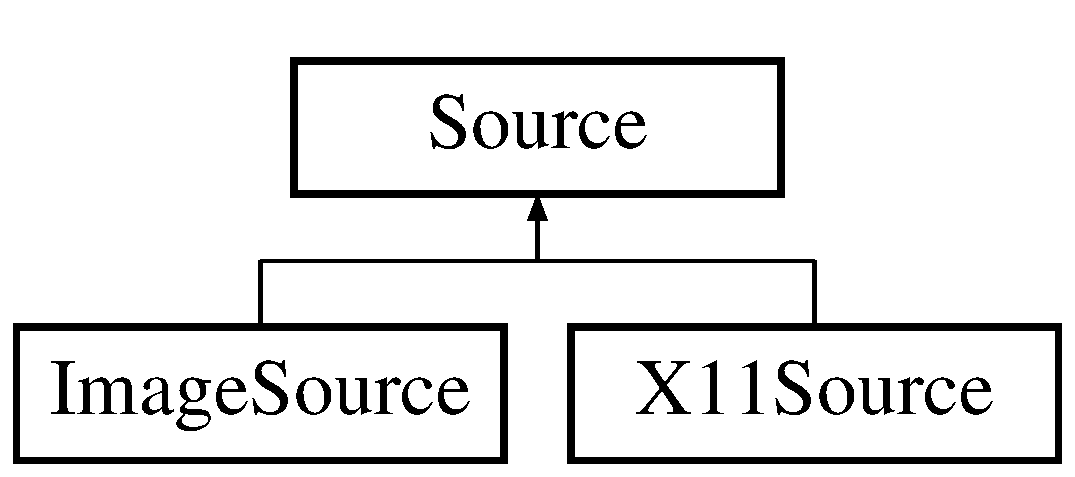
\includegraphics[height=2.000000cm]{classSource}
\end{center}
\end{figure}
\subsubsection*{\-Public \-Member \-Functions}
\begin{DoxyCompactItemize}
\item 
\hyperlink{classSource_a660c0a4b8b8f8402568bef86f2cb2fbb}{\-Source} ()
\item 
\hyperlink{classSource_ac5104a4d66641ae529419b47da4a1473}{$\sim$\-Source} ()
\item 
int \hyperlink{classSource_a57fa5355c01ffdd49d48331b5f304535}{get\-Width} ()
\item 
int \hyperlink{classSource_a1a3e7f05482421bb452f4a6e279a3a19}{get\-Height} ()
\item 
imglib\-::\-Image$<$ float $>$ \& \hyperlink{classSource_aae57269d415b165dfdb91266fc6846ff}{get\-Image} ()
\item 
void \hyperlink{classSource_ac14305006174296199fcbb4fb7e864f8}{set\-Response\-Curve} (string)
\item 
void \hyperlink{classSource_a9a58eb483f03b8778e2058cb4657c3c1}{set\-Whitepoint} (\hyperlink{structrgb}{rgb} wp)
\item 
void \hyperlink{classSource_ac6b164894dc462ea9e5eeb7a96fb62d3}{set\-Exposure} (double exp)
\item 
virtual bool \hyperlink{classSource_acc6f90436f56986b5d261c2408bc1196}{has\-New\-Data} ()=0
\item 
virtual void \hyperlink{classSource_a22e791e3c667fe6d65fa79b30ddc44da}{acquire} ()=0
\item 
void \hyperlink{classSource_ab6174d1cf0bf11ec04a3ff24f75b4f81}{start} ()
\item 
void \hyperlink{classSource_af6025573f44c8fb0485571642a8a0db3}{stop} ()
\end{DoxyCompactItemize}
\subsubsection*{\-Protected \-Types}
\begin{DoxyCompactItemize}
\item 
enum \{ \hyperlink{classSource_af23502cf09ec17790808c30d6a3bca74a9710d90a77764c4d2611decfe6ebe4c8}{\-R\-E\-S\-P\-O\-N\-S\-E\-\_\-\-L\-I\-N\-E\-A\-R}, 
\hyperlink{classSource_af23502cf09ec17790808c30d6a3bca74adef7a29570e1ca10883106b596074f4f}{\-R\-E\-S\-P\-O\-N\-S\-E\-\_\-\-S\-R\-G\-B}, 
\hyperlink{classSource_af23502cf09ec17790808c30d6a3bca74acaa89d52dfe2ddb82eded218d03cb2de}{\-R\-E\-S\-P\-O\-N\-S\-E\-\_\-\-F\-I\-L\-E}
 \}
\end{DoxyCompactItemize}
\subsubsection*{\-Protected \-Member \-Functions}
\begin{DoxyCompactItemize}
\item 
void \hyperlink{classSource_ad2d73e4aaeca3f7c60858ecf165e00ab}{load\-Response\-Curve} (string filename)
\item 
void \hyperlink{classSource_aadcf801d1046197fc00144655ddf2732}{normalize\-Response} ()
\item 
double \hyperlink{classSource_a81708a4890a1077a02091ba4260262e8}{linearize} (double value, int channel)
\item 
imglib\-::\-Image$<$ float $>$ \& \hyperlink{classSource_a754e6d21c1afcde0292fc8648bd3934a}{linearize} (imglib\-::\-Image$<$ float $>$ \&)
\end{DoxyCompactItemize}
\subsubsection*{\-Static \-Protected \-Member \-Functions}
\begin{DoxyCompactItemize}
\item 
static void $\ast$ \hyperlink{classSource_a65c60f259db311b04c5d411507c6e175}{start\-\_\-thread} (void $\ast$ptr)
\end{DoxyCompactItemize}
\subsubsection*{\-Protected \-Attributes}
\begin{DoxyCompactItemize}
\item 
bool \hyperlink{classSource_a83d6fedd341d8b250233c3488b8e231b}{running}
\item 
bool \hyperlink{classSource_a045913a06b522caf5e2766c7dd560b64}{locked}
\item 
imglib\-::\-Image$<$ float $>$ \hyperlink{classSource_a411290665ab67a6a1c7ad4f52d06e9de}{image\-Buffer}
\item 
imglib\-::\-Image$<$ float $>$ \hyperlink{classSource_ad9a7cd1515ec31d5d8cb68896b967816}{image\-Copy}
\item 
int \hyperlink{classSource_a4cead9f95c3faf3f77ea3854ab2a7f10}{width}
\item 
int \hyperlink{classSource_aecf9a912fc51ff3d6c80fcfd871a8484}{height}
\item 
double \hyperlink{classSource_aa35ec9b311cf81ed05fea0ecfe19f42c}{exposure}
\item 
\hyperlink{structrgb}{rgb} \hyperlink{classSource_a08ffcbc3671134eeac92c71de15c2e37}{whitepoint}
\item 
int \hyperlink{classSource_a4bd6ea1c9d9b406dcc5607296083a944}{response\-Size}
\item 
double $\ast$ \hyperlink{classSource_ad303f13ffdd7db993c78843c0c4042e9}{response\-Curve} \mbox{[}3\mbox{]}
\item 
enum \-Source\-:: \{ ... \}  \hyperlink{classSource_ae1511ec3482e54664e82697faab80885}{response\-Type}
\item 
double \hyperlink{classSource_a43f5162009aceeca7fbfddcee7c53eff}{update\-Rate}
\end{DoxyCompactItemize}


\subsubsection{\-Detailed \-Description}
\-Acquires and linearizes images. 

\begin{DoxyAuthor}{\-Author}
\-Manuel \-Jerger $<$\href{mailto:nom@nomnom.de}{\tt nom@nomnom.\-de}$>$
\end{DoxyAuthor}
\-The \hyperlink{classSource}{\-Source} class acquires, linearizes and returns images. \-Supports threading. 

\subsubsection{\-Member \-Enumeration \-Documentation}
\hypertarget{classSource_af23502cf09ec17790808c30d6a3bca74}{\paragraph[{anonymous enum}]{\setlength{\rightskip}{0pt plus 5cm}anonymous enum\hspace{0.3cm}{\ttfamily  \mbox{[}protected\mbox{]}}}}\label{classSource_af23502cf09ec17790808c30d6a3bca74}
\begin{Desc}
\item[\-Enumerator\-: ]\par
\begin{description}
\index{\-R\-E\-S\-P\-O\-N\-S\-E\-\_\-\-L\-I\-N\-E\-A\-R@{\-R\-E\-S\-P\-O\-N\-S\-E\-\_\-\-L\-I\-N\-E\-A\-R}!\-Source@{\-Source}}\index{\-Source@{\-Source}!\-R\-E\-S\-P\-O\-N\-S\-E\-\_\-\-L\-I\-N\-E\-A\-R@{\-R\-E\-S\-P\-O\-N\-S\-E\-\_\-\-L\-I\-N\-E\-A\-R}}\item[{\em 
\hypertarget{classSource_af23502cf09ec17790808c30d6a3bca74a9710d90a77764c4d2611decfe6ebe4c8}{\-R\-E\-S\-P\-O\-N\-S\-E\-\_\-\-L\-I\-N\-E\-A\-R}\label{classSource_af23502cf09ec17790808c30d6a3bca74a9710d90a77764c4d2611decfe6ebe4c8}
}]\index{\-R\-E\-S\-P\-O\-N\-S\-E\-\_\-\-S\-R\-G\-B@{\-R\-E\-S\-P\-O\-N\-S\-E\-\_\-\-S\-R\-G\-B}!\-Source@{\-Source}}\index{\-Source@{\-Source}!\-R\-E\-S\-P\-O\-N\-S\-E\-\_\-\-S\-R\-G\-B@{\-R\-E\-S\-P\-O\-N\-S\-E\-\_\-\-S\-R\-G\-B}}\item[{\em 
\hypertarget{classSource_af23502cf09ec17790808c30d6a3bca74adef7a29570e1ca10883106b596074f4f}{\-R\-E\-S\-P\-O\-N\-S\-E\-\_\-\-S\-R\-G\-B}\label{classSource_af23502cf09ec17790808c30d6a3bca74adef7a29570e1ca10883106b596074f4f}
}]\index{\-R\-E\-S\-P\-O\-N\-S\-E\-\_\-\-F\-I\-L\-E@{\-R\-E\-S\-P\-O\-N\-S\-E\-\_\-\-F\-I\-L\-E}!\-Source@{\-Source}}\index{\-Source@{\-Source}!\-R\-E\-S\-P\-O\-N\-S\-E\-\_\-\-F\-I\-L\-E@{\-R\-E\-S\-P\-O\-N\-S\-E\-\_\-\-F\-I\-L\-E}}\item[{\em 
\hypertarget{classSource_af23502cf09ec17790808c30d6a3bca74acaa89d52dfe2ddb82eded218d03cb2de}{\-R\-E\-S\-P\-O\-N\-S\-E\-\_\-\-F\-I\-L\-E}\label{classSource_af23502cf09ec17790808c30d6a3bca74acaa89d52dfe2ddb82eded218d03cb2de}
}]\end{description}
\end{Desc}



\subsubsection{\-Constructor \& \-Destructor \-Documentation}
\hypertarget{classSource_a660c0a4b8b8f8402568bef86f2cb2fbb}{\index{\-Source@{\-Source}!\-Source@{\-Source}}
\index{\-Source@{\-Source}!Source@{\-Source}}
\paragraph[{\-Source}]{\setlength{\rightskip}{0pt plus 5cm}{\bf \-Source\-::\-Source} (
\begin{DoxyParamCaption}
{}
\end{DoxyParamCaption}
)}}\label{classSource_a660c0a4b8b8f8402568bef86f2cb2fbb}
\begin{DoxyAuthor}{\-Author}
\-Manuel \-Jerger $<$\href{mailto:nom@nomnom.de}{\tt nom@nomnom.\-de}$>$
\end{DoxyAuthor}
\-The \hyperlink{classSource}{\-Source} class acquires, linearizes and returns images. \-Supports threading. \hypertarget{classSource_ac5104a4d66641ae529419b47da4a1473}{\index{\-Source@{\-Source}!$\sim$\-Source@{$\sim$\-Source}}
\index{$\sim$\-Source@{$\sim$\-Source}!Source@{\-Source}}
\paragraph[{$\sim$\-Source}]{\setlength{\rightskip}{0pt plus 5cm}{\bf \-Source\-::$\sim$\-Source} (
\begin{DoxyParamCaption}
{}
\end{DoxyParamCaption}
)}}\label{classSource_ac5104a4d66641ae529419b47da4a1473}


\subsubsection{\-Member \-Function \-Documentation}
\hypertarget{classSource_a22e791e3c667fe6d65fa79b30ddc44da}{\index{\-Source@{\-Source}!acquire@{acquire}}
\index{acquire@{acquire}!Source@{\-Source}}
\paragraph[{acquire}]{\setlength{\rightskip}{0pt plus 5cm}virtual void {\bf \-Source\-::acquire} (
\begin{DoxyParamCaption}
{}
\end{DoxyParamCaption}
)\hspace{0.3cm}{\ttfamily  \mbox{[}pure virtual\mbox{]}}}}\label{classSource_a22e791e3c667fe6d65fa79b30ddc44da}


\-Implemented in \hyperlink{classX11Source_a1f1e97d8c02bfe6d5d84fb06a06125ba}{\-X11\-Source}, and \hyperlink{classImageSource_ad969a45dd3dbda08b9a73f50ada50dfb}{\-Image\-Source}.

\hypertarget{classSource_a1a3e7f05482421bb452f4a6e279a3a19}{\index{\-Source@{\-Source}!get\-Height@{get\-Height}}
\index{get\-Height@{get\-Height}!Source@{\-Source}}
\paragraph[{get\-Height}]{\setlength{\rightskip}{0pt plus 5cm}int {\bf \-Source\-::get\-Height} (
\begin{DoxyParamCaption}
{}
\end{DoxyParamCaption}
)\hspace{0.3cm}{\ttfamily  \mbox{[}inline\mbox{]}}}}\label{classSource_a1a3e7f05482421bb452f4a6e279a3a19}
\hypertarget{classSource_aae57269d415b165dfdb91266fc6846ff}{\index{\-Source@{\-Source}!get\-Image@{get\-Image}}
\index{get\-Image@{get\-Image}!Source@{\-Source}}
\paragraph[{get\-Image}]{\setlength{\rightskip}{0pt plus 5cm}imglib\-::\-Image$<$ float $>$ \& {\bf \-Source\-::get\-Image} (
\begin{DoxyParamCaption}
{}
\end{DoxyParamCaption}
)}}\label{classSource_aae57269d415b165dfdb91266fc6846ff}
\hypertarget{classSource_a57fa5355c01ffdd49d48331b5f304535}{\index{\-Source@{\-Source}!get\-Width@{get\-Width}}
\index{get\-Width@{get\-Width}!Source@{\-Source}}
\paragraph[{get\-Width}]{\setlength{\rightskip}{0pt plus 5cm}int {\bf \-Source\-::get\-Width} (
\begin{DoxyParamCaption}
{}
\end{DoxyParamCaption}
)\hspace{0.3cm}{\ttfamily  \mbox{[}inline\mbox{]}}}}\label{classSource_a57fa5355c01ffdd49d48331b5f304535}
\hypertarget{classSource_acc6f90436f56986b5d261c2408bc1196}{\index{\-Source@{\-Source}!has\-New\-Data@{has\-New\-Data}}
\index{has\-New\-Data@{has\-New\-Data}!Source@{\-Source}}
\paragraph[{has\-New\-Data}]{\setlength{\rightskip}{0pt plus 5cm}virtual bool {\bf \-Source\-::has\-New\-Data} (
\begin{DoxyParamCaption}
{}
\end{DoxyParamCaption}
)\hspace{0.3cm}{\ttfamily  \mbox{[}pure virtual\mbox{]}}}}\label{classSource_acc6f90436f56986b5d261c2408bc1196}


\-Implemented in \hyperlink{classX11Source_aa9b91f2a4a6db72b9391bc43d8f73944}{\-X11\-Source}, and \hyperlink{classImageSource_ab65bd864ba3c7961479ec2ad3b1ff163}{\-Image\-Source}.

\hypertarget{classSource_a81708a4890a1077a02091ba4260262e8}{\index{\-Source@{\-Source}!linearize@{linearize}}
\index{linearize@{linearize}!Source@{\-Source}}
\paragraph[{linearize}]{\setlength{\rightskip}{0pt plus 5cm}double {\bf \-Source\-::linearize} (
\begin{DoxyParamCaption}
\item[{double}]{value, }
\item[{int}]{channel}
\end{DoxyParamCaption}
)\hspace{0.3cm}{\ttfamily  \mbox{[}protected\mbox{]}}}}\label{classSource_a81708a4890a1077a02091ba4260262e8}
\-Linearizes a single value using the supplied response curve and maps the white point. \hypertarget{classSource_a754e6d21c1afcde0292fc8648bd3934a}{\index{\-Source@{\-Source}!linearize@{linearize}}
\index{linearize@{linearize}!Source@{\-Source}}
\paragraph[{linearize}]{\setlength{\rightskip}{0pt plus 5cm}imglib\-::\-Image$<$ float $>$ \& {\bf \-Source\-::linearize} (
\begin{DoxyParamCaption}
\item[{imglib\-::\-Image$<$ float $>$ \&}]{\-A}
\end{DoxyParamCaption}
)\hspace{0.3cm}{\ttfamily  \mbox{[}protected\mbox{]}}}}\label{classSource_a754e6d21c1afcde0292fc8648bd3934a}
\-Linearizes an image using the supplied response curve and maps the white point. \hypertarget{classSource_ad2d73e4aaeca3f7c60858ecf165e00ab}{\index{\-Source@{\-Source}!load\-Response\-Curve@{load\-Response\-Curve}}
\index{load\-Response\-Curve@{load\-Response\-Curve}!Source@{\-Source}}
\paragraph[{load\-Response\-Curve}]{\setlength{\rightskip}{0pt plus 5cm}void {\bf \-Source\-::load\-Response\-Curve} (
\begin{DoxyParamCaption}
\item[{string}]{filename}
\end{DoxyParamCaption}
)\hspace{0.3cm}{\ttfamily  \mbox{[}protected\mbox{]}}}}\label{classSource_ad2d73e4aaeca3f7c60858ecf165e00ab}
loads an three-\/channel response curve (either .m format created with hdrcalibrate, or a white-\/space separated three-\/column list) \hypertarget{classSource_aadcf801d1046197fc00144655ddf2732}{\index{\-Source@{\-Source}!normalize\-Response@{normalize\-Response}}
\index{normalize\-Response@{normalize\-Response}!Source@{\-Source}}
\paragraph[{normalize\-Response}]{\setlength{\rightskip}{0pt plus 5cm}void {\bf \-Source\-::normalize\-Response} (
\begin{DoxyParamCaption}
{}
\end{DoxyParamCaption}
)\hspace{0.3cm}{\ttfamily  \mbox{[}protected\mbox{]}}}}\label{classSource_aadcf801d1046197fc00144655ddf2732}
\-Normalizes the response curve so the image values fits in the range (0\-:1). \-The largest value of the three channels of the response curve is mapped to 1.\-0. \-The largest value at index 0 is mapped to zero, so we have no positive offset. \-All three channels are scaled with the same value to preserve the relative relation. \hypertarget{classSource_ac6b164894dc462ea9e5eeb7a96fb62d3}{\index{\-Source@{\-Source}!set\-Exposure@{set\-Exposure}}
\index{set\-Exposure@{set\-Exposure}!Source@{\-Source}}
\paragraph[{set\-Exposure}]{\setlength{\rightskip}{0pt plus 5cm}void {\bf \-Source\-::set\-Exposure} (
\begin{DoxyParamCaption}
\item[{double}]{exp}
\end{DoxyParamCaption}
)}}\label{classSource_ac6b164894dc462ea9e5eeb7a96fb62d3}
\hypertarget{classSource_ac14305006174296199fcbb4fb7e864f8}{\index{\-Source@{\-Source}!set\-Response\-Curve@{set\-Response\-Curve}}
\index{set\-Response\-Curve@{set\-Response\-Curve}!Source@{\-Source}}
\paragraph[{set\-Response\-Curve}]{\setlength{\rightskip}{0pt plus 5cm}void {\bf \-Source\-::set\-Response\-Curve} (
\begin{DoxyParamCaption}
\item[{string}]{reponse\-Str}
\end{DoxyParamCaption}
)}}\label{classSource_ac14305006174296199fcbb4fb7e864f8}
\hypertarget{classSource_a9a58eb483f03b8778e2058cb4657c3c1}{\index{\-Source@{\-Source}!set\-Whitepoint@{set\-Whitepoint}}
\index{set\-Whitepoint@{set\-Whitepoint}!Source@{\-Source}}
\paragraph[{set\-Whitepoint}]{\setlength{\rightskip}{0pt plus 5cm}void {\bf \-Source\-::set\-Whitepoint} (
\begin{DoxyParamCaption}
\item[{{\bf rgb}}]{wp}
\end{DoxyParamCaption}
)}}\label{classSource_a9a58eb483f03b8778e2058cb4657c3c1}
\hypertarget{classSource_ab6174d1cf0bf11ec04a3ff24f75b4f81}{\index{\-Source@{\-Source}!start@{start}}
\index{start@{start}!Source@{\-Source}}
\paragraph[{start}]{\setlength{\rightskip}{0pt plus 5cm}void {\bf \-Source\-::start} (
\begin{DoxyParamCaption}
{}
\end{DoxyParamCaption}
)}}\label{classSource_ab6174d1cf0bf11ec04a3ff24f75b4f81}
\hypertarget{classSource_a65c60f259db311b04c5d411507c6e175}{\index{\-Source@{\-Source}!start\-\_\-thread@{start\-\_\-thread}}
\index{start\-\_\-thread@{start\-\_\-thread}!Source@{\-Source}}
\paragraph[{start\-\_\-thread}]{\setlength{\rightskip}{0pt plus 5cm}void $\ast$ {\bf \-Source\-::start\-\_\-thread} (
\begin{DoxyParamCaption}
\item[{void $\ast$}]{ptr}
\end{DoxyParamCaption}
)\hspace{0.3cm}{\ttfamily  \mbox{[}static, protected\mbox{]}}}}\label{classSource_a65c60f259db311b04c5d411507c6e175}
\hypertarget{classSource_af6025573f44c8fb0485571642a8a0db3}{\index{\-Source@{\-Source}!stop@{stop}}
\index{stop@{stop}!Source@{\-Source}}
\paragraph[{stop}]{\setlength{\rightskip}{0pt plus 5cm}void {\bf \-Source\-::stop} (
\begin{DoxyParamCaption}
{}
\end{DoxyParamCaption}
)}}\label{classSource_af6025573f44c8fb0485571642a8a0db3}


\subsubsection{\-Field \-Documentation}
\hypertarget{classSource_aa35ec9b311cf81ed05fea0ecfe19f42c}{\index{\-Source@{\-Source}!exposure@{exposure}}
\index{exposure@{exposure}!Source@{\-Source}}
\paragraph[{exposure}]{\setlength{\rightskip}{0pt plus 5cm}double {\bf \-Source\-::exposure}\hspace{0.3cm}{\ttfamily  \mbox{[}protected\mbox{]}}}}\label{classSource_aa35ec9b311cf81ed05fea0ecfe19f42c}
\hypertarget{classSource_aecf9a912fc51ff3d6c80fcfd871a8484}{\index{\-Source@{\-Source}!height@{height}}
\index{height@{height}!Source@{\-Source}}
\paragraph[{height}]{\setlength{\rightskip}{0pt plus 5cm}int {\bf \-Source\-::height}\hspace{0.3cm}{\ttfamily  \mbox{[}protected\mbox{]}}}}\label{classSource_aecf9a912fc51ff3d6c80fcfd871a8484}
\hypertarget{classSource_a411290665ab67a6a1c7ad4f52d06e9de}{\index{\-Source@{\-Source}!image\-Buffer@{image\-Buffer}}
\index{image\-Buffer@{image\-Buffer}!Source@{\-Source}}
\paragraph[{image\-Buffer}]{\setlength{\rightskip}{0pt plus 5cm}imglib\-::\-Image$<$float$>$ {\bf \-Source\-::image\-Buffer}\hspace{0.3cm}{\ttfamily  \mbox{[}protected\mbox{]}}}}\label{classSource_a411290665ab67a6a1c7ad4f52d06e9de}
\hypertarget{classSource_ad9a7cd1515ec31d5d8cb68896b967816}{\index{\-Source@{\-Source}!image\-Copy@{image\-Copy}}
\index{image\-Copy@{image\-Copy}!Source@{\-Source}}
\paragraph[{image\-Copy}]{\setlength{\rightskip}{0pt plus 5cm}imglib\-::\-Image$<$float$>$ {\bf \-Source\-::image\-Copy}\hspace{0.3cm}{\ttfamily  \mbox{[}protected\mbox{]}}}}\label{classSource_ad9a7cd1515ec31d5d8cb68896b967816}
\hypertarget{classSource_a045913a06b522caf5e2766c7dd560b64}{\index{\-Source@{\-Source}!locked@{locked}}
\index{locked@{locked}!Source@{\-Source}}
\paragraph[{locked}]{\setlength{\rightskip}{0pt plus 5cm}bool {\bf \-Source\-::locked}\hspace{0.3cm}{\ttfamily  \mbox{[}protected\mbox{]}}}}\label{classSource_a045913a06b522caf5e2766c7dd560b64}
\hypertarget{classSource_ad303f13ffdd7db993c78843c0c4042e9}{\index{\-Source@{\-Source}!response\-Curve@{response\-Curve}}
\index{response\-Curve@{response\-Curve}!Source@{\-Source}}
\paragraph[{response\-Curve}]{\setlength{\rightskip}{0pt plus 5cm}double$\ast$ {\bf \-Source\-::response\-Curve}\mbox{[}3\mbox{]}\hspace{0.3cm}{\ttfamily  \mbox{[}protected\mbox{]}}}}\label{classSource_ad303f13ffdd7db993c78843c0c4042e9}
\hypertarget{classSource_a4bd6ea1c9d9b406dcc5607296083a944}{\index{\-Source@{\-Source}!response\-Size@{response\-Size}}
\index{response\-Size@{response\-Size}!Source@{\-Source}}
\paragraph[{response\-Size}]{\setlength{\rightskip}{0pt plus 5cm}int {\bf \-Source\-::response\-Size}\hspace{0.3cm}{\ttfamily  \mbox{[}protected\mbox{]}}}}\label{classSource_a4bd6ea1c9d9b406dcc5607296083a944}
\hypertarget{classSource_ae1511ec3482e54664e82697faab80885}{\index{\-Source@{\-Source}!response\-Type@{response\-Type}}
\index{response\-Type@{response\-Type}!Source@{\-Source}}
\paragraph[{response\-Type}]{\setlength{\rightskip}{0pt plus 5cm}enum \{ ... \}   {\bf \-Source\-::response\-Type}\hspace{0.3cm}{\ttfamily  \mbox{[}protected\mbox{]}}}}\label{classSource_ae1511ec3482e54664e82697faab80885}
\hypertarget{classSource_a83d6fedd341d8b250233c3488b8e231b}{\index{\-Source@{\-Source}!running@{running}}
\index{running@{running}!Source@{\-Source}}
\paragraph[{running}]{\setlength{\rightskip}{0pt plus 5cm}bool {\bf \-Source\-::running}\hspace{0.3cm}{\ttfamily  \mbox{[}protected\mbox{]}}}}\label{classSource_a83d6fedd341d8b250233c3488b8e231b}
\hypertarget{classSource_a43f5162009aceeca7fbfddcee7c53eff}{\index{\-Source@{\-Source}!update\-Rate@{update\-Rate}}
\index{update\-Rate@{update\-Rate}!Source@{\-Source}}
\paragraph[{update\-Rate}]{\setlength{\rightskip}{0pt plus 5cm}double {\bf \-Source\-::update\-Rate}\hspace{0.3cm}{\ttfamily  \mbox{[}protected\mbox{]}}}}\label{classSource_a43f5162009aceeca7fbfddcee7c53eff}
\hypertarget{classSource_a08ffcbc3671134eeac92c71de15c2e37}{\index{\-Source@{\-Source}!whitepoint@{whitepoint}}
\index{whitepoint@{whitepoint}!Source@{\-Source}}
\paragraph[{whitepoint}]{\setlength{\rightskip}{0pt plus 5cm}{\bf rgb} {\bf \-Source\-::whitepoint}\hspace{0.3cm}{\ttfamily  \mbox{[}protected\mbox{]}}}}\label{classSource_a08ffcbc3671134eeac92c71de15c2e37}
\hypertarget{classSource_a4cead9f95c3faf3f77ea3854ab2a7f10}{\index{\-Source@{\-Source}!width@{width}}
\index{width@{width}!Source@{\-Source}}
\paragraph[{width}]{\setlength{\rightskip}{0pt plus 5cm}int {\bf \-Source\-::width}\hspace{0.3cm}{\ttfamily  \mbox{[}protected\mbox{]}}}}\label{classSource_a4cead9f95c3faf3f77ea3854ab2a7f10}


\-The documentation for this class was generated from the following files\-:\begin{DoxyCompactItemize}
\item 
src/\hyperlink{source_8h}{source.\-h}\item 
src/\hyperlink{source_8cpp}{source.\-cpp}\end{DoxyCompactItemize}

\hypertarget{classSticks}{\subsection{\-Sticks \-Class \-Reference}
\label{classSticks}\index{\-Sticks@{\-Sticks}}
}


\-Our sticks lighting system.  




{\ttfamily \#include $<$sticks.\-h$>$}

\-Inheritance diagram for \-Sticks\-:\begin{figure}[H]
\begin{center}
\leavevmode
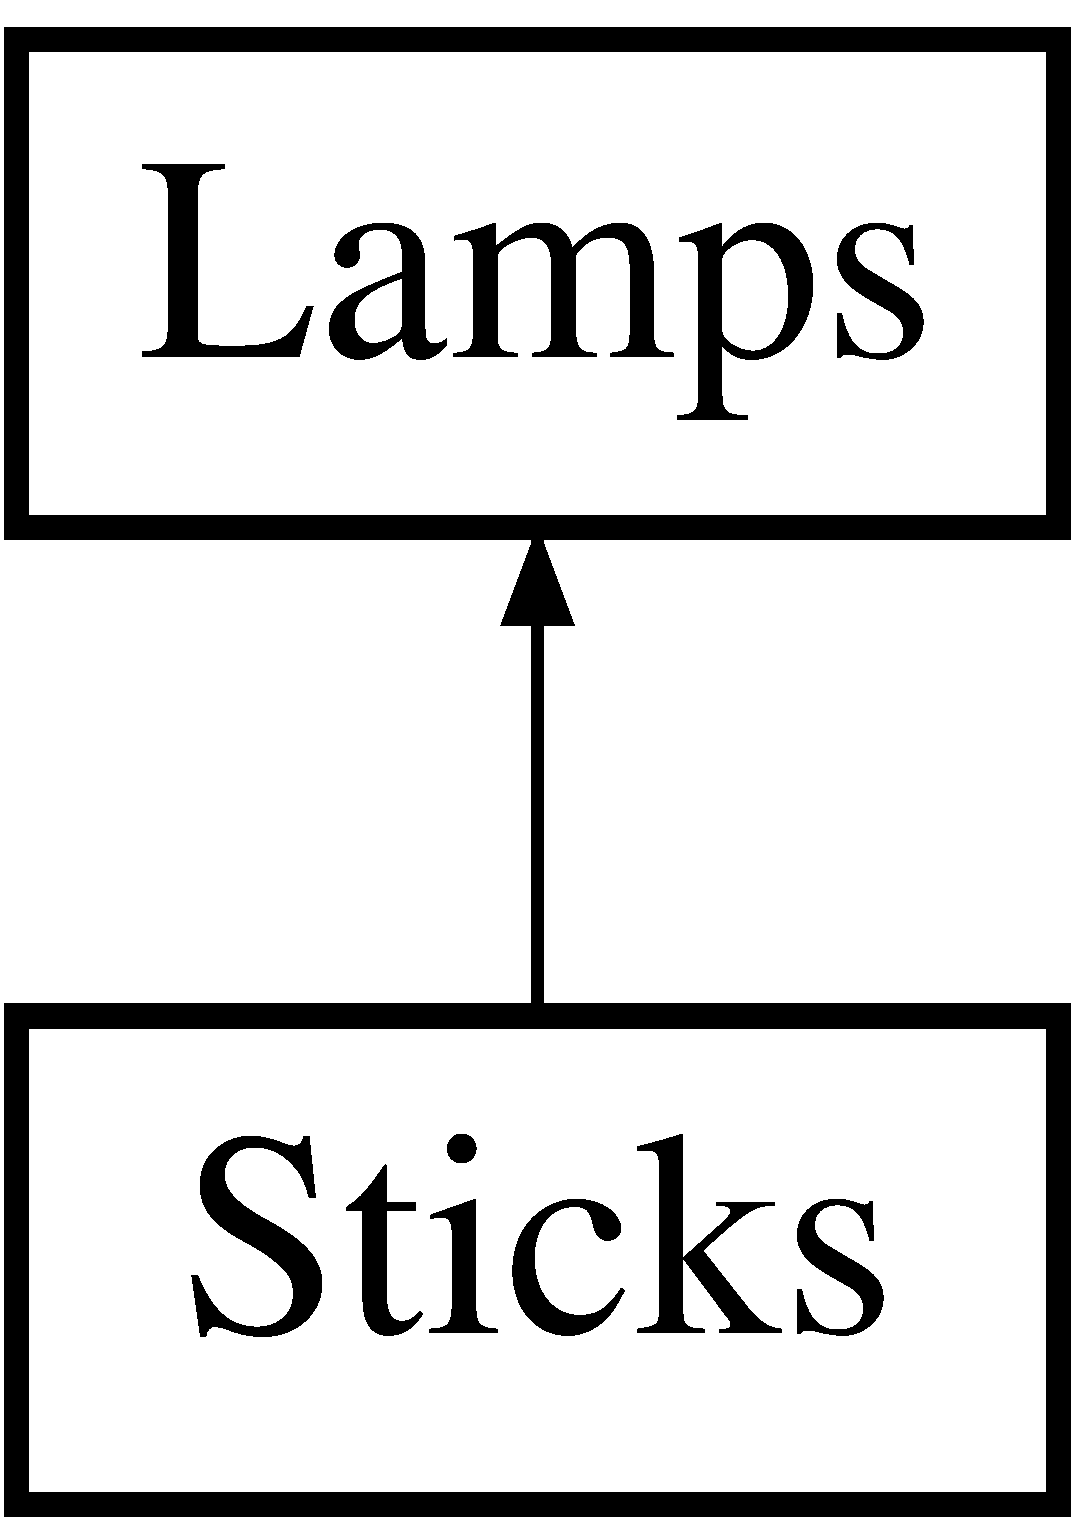
\includegraphics[height=2.000000cm]{classSticks}
\end{center}
\end{figure}
\subsubsection*{\-Data \-Structures}
\begin{DoxyCompactItemize}
\item 
struct \hyperlink{structSticks_1_1params}{params}
\begin{DoxyCompactList}\small\item\em \-Configuration of our lighting system. \end{DoxyCompactList}\end{DoxyCompactItemize}
\subsubsection*{\-Public \-Member \-Functions}
\begin{DoxyCompactItemize}
\item 
\hyperlink{classSticks_ac82542df85c5dbfd68c84687af6591fd}{\-Sticks} (\hyperlink{structSticks_1_1params}{params} \hyperlink{classSticks_ad77454176517e28c47a4eba37c307d02}{config})
\item 
\hyperlink{classSticks_ac2c945078a4add60443f7ad3caaa377d}{\-Sticks} (int segment\-Size, string device, double rate)
\item 
\hyperlink{classSticks_ac62f6318efd98f6f636ed9bafb51db21}{$\sim$\-Sticks} ()
\item 
\hyperlink{structSticks_1_1params}{params} \hyperlink{classSticks_a54a8ba2fb5eacdc1b529bd92efbe4475}{get\-Config} ()
\item 
bool \hyperlink{classSticks_a7baa38ffec8cecc9ffebf99010db1e92}{has\-R\-G\-B\-Lamps} ()
\item 
int \hyperlink{classSticks_a2c87f49e1415691e50c84f7f071f07a9}{get\-Num\-R\-G\-B\-Lamps} ()
\item 
void \hyperlink{classSticks_a6500a23f49137753c03d61ca6ecbc727}{set\-R\-G\-B\-Value} (int lamp\-I\-D, \hyperlink{structrgb}{rgb})
\item 
\hyperlink{structrgb}{rgb} \hyperlink{classSticks_a12d3d039d913d36180bfe7820115f731}{get\-R\-G\-B\-Value} (int lamp\-I\-D)
\item 
void \hyperlink{classSticks_aaf3b58bc647d0d6c31825e64b4398281}{set\-All\-R\-G\-B} (\hyperlink{structrgb}{rgb})
\item 
int \hyperlink{classSticks_af6af53b803183ff0c81b119e9726fac0}{get\-Num\-Sticks} ()
\item 
int \hyperlink{classSticks_ad50d1570ca4a0837b448381bc738d422}{get\-Stick\-Length} (int lamp\-I\-D)
\item 
void \hyperlink{classSticks_a84810306863a52b6ad8fdb790bec1103}{set\-Stick\-R\-G\-B\-Value} (int stick\-I\-D, int lamp\-I\-D, \hyperlink{structrgb}{rgb})
\item 
\hyperlink{structrgb}{rgb} \hyperlink{classSticks_a9900abe23c463b65a8ef05dc9f63c035}{get\-Stick\-R\-G\-B\-Value} (int stick\-I\-D, int lamp\-I\-D)
\item 
void \hyperlink{classSticks_aa3027db7aa82003ed782961f26844f22}{set\-Stick\-Channel\-Value} (int stick\-I\-D, int stick\-Lamp\-I\-D, double val, int channel)
\item 
void \hyperlink{classSticks_ad2740b596bbeb3c24da66272ae290372}{set\-All\-Channel} (double val, int channel)
\item 
bool \hyperlink{classSticks_a6fc1fb933fbe6ce05ba88ef83322a0f1}{is\-Ready} ()
\item 
bool \hyperlink{classSticks_aa19dfda62c22c44cd4bda1e3abe3f0af}{send} ()
\end{DoxyCompactItemize}
\subsubsection*{\-Private \-Member \-Functions}
\begin{DoxyCompactItemize}
\item 
void \hyperlink{classSticks_a6db1929d8fc43c94377c6dbfafe5f55f}{init} ()
\item 
unsigned char \hyperlink{classSticks_abdbc514786c495286d6e0c6a83e33150}{map\-Mono} (double brightness)
\end{DoxyCompactItemize}
\subsubsection*{\-Private \-Attributes}
\begin{DoxyCompactItemize}
\item 
\hyperlink{structSticks_1_1params}{params} \hyperlink{classSticks_ad77454176517e28c47a4eba37c307d02}{config}
\item 
int \hyperlink{classSticks_a4f14013508b750816b5acfe029be7b6a}{strip\-Lengths} \mbox{[}8\mbox{]}
\item 
int \hyperlink{classSticks_a22fe70b7d473809d323df75cadf2581c}{max\-Strip\-Length}
\item 
int \hyperlink{classSticks_aee9f9b761688fb38972458e3d0c454ff}{real\-Strip\-Length}
\item 
int \hyperlink{classSticks_ab612d8d5a4dbc6e195f878dfa40f321d}{max\-Num\-Segs}
\item 
vector$<$ unsigned char $>$ \hyperlink{classSticks_add99fb5e5c554f78bd5fed3e0613b466}{raw\-Values} \mbox{[}8\mbox{]}\mbox{[}3\mbox{]}
\item 
int \hyperlink{classSticks_ae7c50972f44a386b5cd4dcf182f7550a}{serial\-Port}
\end{DoxyCompactItemize}


\subsubsection{\-Detailed \-Description}
\-Our sticks lighting system. 

\subsubsection{\-Constructor \& \-Destructor \-Documentation}
\hypertarget{classSticks_ac82542df85c5dbfd68c84687af6591fd}{\index{\-Sticks@{\-Sticks}!\-Sticks@{\-Sticks}}
\index{\-Sticks@{\-Sticks}!Sticks@{\-Sticks}}
\paragraph[{\-Sticks}]{\setlength{\rightskip}{0pt plus 5cm}{\bf \-Sticks\-::\-Sticks} (
\begin{DoxyParamCaption}
\item[{{\bf params}}]{c}
\end{DoxyParamCaption}
)}}\label{classSticks_ac82542df85c5dbfd68c84687af6591fd}
\begin{DoxyAuthor}{\-Author}
\-Manuel \-Jerger $<$\href{mailto:nom@nomnom.de}{\tt nom@nomnom.\-de}$>$
\end{DoxyAuthor}
\-This class represents our lighting system. \-Controls eight strips of 120 \-W\-S2812 \-L\-E\-Ds via the \-Teensy microcontroller over the serial port. \-L\-E\-Ds on a strip are segmented into a equal sized patches. \hypertarget{classSticks_ac2c945078a4add60443f7ad3caaa377d}{\index{\-Sticks@{\-Sticks}!\-Sticks@{\-Sticks}}
\index{\-Sticks@{\-Sticks}!Sticks@{\-Sticks}}
\paragraph[{\-Sticks}]{\setlength{\rightskip}{0pt plus 5cm}{\bf \-Sticks\-::\-Sticks} (
\begin{DoxyParamCaption}
\item[{int}]{segment\-Size, }
\item[{string}]{device, }
\item[{double}]{rate}
\end{DoxyParamCaption}
)}}\label{classSticks_ac2c945078a4add60443f7ad3caaa377d}
\hypertarget{classSticks_ac62f6318efd98f6f636ed9bafb51db21}{\index{\-Sticks@{\-Sticks}!$\sim$\-Sticks@{$\sim$\-Sticks}}
\index{$\sim$\-Sticks@{$\sim$\-Sticks}!Sticks@{\-Sticks}}
\paragraph[{$\sim$\-Sticks}]{\setlength{\rightskip}{0pt plus 5cm}{\bf \-Sticks\-::$\sim$\-Sticks} (
\begin{DoxyParamCaption}
{}
\end{DoxyParamCaption}
)}}\label{classSticks_ac62f6318efd98f6f636ed9bafb51db21}


\subsubsection{\-Member \-Function \-Documentation}
\hypertarget{classSticks_a54a8ba2fb5eacdc1b529bd92efbe4475}{\index{\-Sticks@{\-Sticks}!get\-Config@{get\-Config}}
\index{get\-Config@{get\-Config}!Sticks@{\-Sticks}}
\paragraph[{get\-Config}]{\setlength{\rightskip}{0pt plus 5cm}{\bf \-Sticks\-::params} {\bf \-Sticks\-::get\-Config} (
\begin{DoxyParamCaption}
{}
\end{DoxyParamCaption}
)}}\label{classSticks_a54a8ba2fb5eacdc1b529bd92efbe4475}
\hypertarget{classSticks_a2c87f49e1415691e50c84f7f071f07a9}{\index{\-Sticks@{\-Sticks}!get\-Num\-R\-G\-B\-Lamps@{get\-Num\-R\-G\-B\-Lamps}}
\index{get\-Num\-R\-G\-B\-Lamps@{get\-Num\-R\-G\-B\-Lamps}!Sticks@{\-Sticks}}
\paragraph[{get\-Num\-R\-G\-B\-Lamps}]{\setlength{\rightskip}{0pt plus 5cm}int {\bf \-Sticks\-::get\-Num\-R\-G\-B\-Lamps} (
\begin{DoxyParamCaption}
{}
\end{DoxyParamCaption}
)}}\label{classSticks_a2c87f49e1415691e50c84f7f071f07a9}
\hypertarget{classSticks_af6af53b803183ff0c81b119e9726fac0}{\index{\-Sticks@{\-Sticks}!get\-Num\-Sticks@{get\-Num\-Sticks}}
\index{get\-Num\-Sticks@{get\-Num\-Sticks}!Sticks@{\-Sticks}}
\paragraph[{get\-Num\-Sticks}]{\setlength{\rightskip}{0pt plus 5cm}int {\bf \-Sticks\-::get\-Num\-Sticks} (
\begin{DoxyParamCaption}
{}
\end{DoxyParamCaption}
)}}\label{classSticks_af6af53b803183ff0c81b119e9726fac0}
\hypertarget{classSticks_a12d3d039d913d36180bfe7820115f731}{\index{\-Sticks@{\-Sticks}!get\-R\-G\-B\-Value@{get\-R\-G\-B\-Value}}
\index{get\-R\-G\-B\-Value@{get\-R\-G\-B\-Value}!Sticks@{\-Sticks}}
\paragraph[{get\-R\-G\-B\-Value}]{\setlength{\rightskip}{0pt plus 5cm}{\bf rgb} {\bf \-Sticks\-::get\-R\-G\-B\-Value} (
\begin{DoxyParamCaption}
\item[{int}]{lamp\-I\-D}
\end{DoxyParamCaption}
)}}\label{classSticks_a12d3d039d913d36180bfe7820115f731}
\hypertarget{classSticks_ad50d1570ca4a0837b448381bc738d422}{\index{\-Sticks@{\-Sticks}!get\-Stick\-Length@{get\-Stick\-Length}}
\index{get\-Stick\-Length@{get\-Stick\-Length}!Sticks@{\-Sticks}}
\paragraph[{get\-Stick\-Length}]{\setlength{\rightskip}{0pt plus 5cm}int {\bf \-Sticks\-::get\-Stick\-Length} (
\begin{DoxyParamCaption}
\item[{int}]{lamp\-I\-D}
\end{DoxyParamCaption}
)}}\label{classSticks_ad50d1570ca4a0837b448381bc738d422}
\hypertarget{classSticks_a9900abe23c463b65a8ef05dc9f63c035}{\index{\-Sticks@{\-Sticks}!get\-Stick\-R\-G\-B\-Value@{get\-Stick\-R\-G\-B\-Value}}
\index{get\-Stick\-R\-G\-B\-Value@{get\-Stick\-R\-G\-B\-Value}!Sticks@{\-Sticks}}
\paragraph[{get\-Stick\-R\-G\-B\-Value}]{\setlength{\rightskip}{0pt plus 5cm}{\bf rgb} {\bf \-Sticks\-::get\-Stick\-R\-G\-B\-Value} (
\begin{DoxyParamCaption}
\item[{int}]{stick\-I\-D, }
\item[{int}]{lamp\-I\-D}
\end{DoxyParamCaption}
)}}\label{classSticks_a9900abe23c463b65a8ef05dc9f63c035}
\hypertarget{classSticks_a7baa38ffec8cecc9ffebf99010db1e92}{\index{\-Sticks@{\-Sticks}!has\-R\-G\-B\-Lamps@{has\-R\-G\-B\-Lamps}}
\index{has\-R\-G\-B\-Lamps@{has\-R\-G\-B\-Lamps}!Sticks@{\-Sticks}}
\paragraph[{has\-R\-G\-B\-Lamps}]{\setlength{\rightskip}{0pt plus 5cm}bool {\bf \-Sticks\-::has\-R\-G\-B\-Lamps} (
\begin{DoxyParamCaption}
{}
\end{DoxyParamCaption}
)}}\label{classSticks_a7baa38ffec8cecc9ffebf99010db1e92}
\hypertarget{classSticks_a6db1929d8fc43c94377c6dbfafe5f55f}{\index{\-Sticks@{\-Sticks}!init@{init}}
\index{init@{init}!Sticks@{\-Sticks}}
\paragraph[{init}]{\setlength{\rightskip}{0pt plus 5cm}void {\bf \-Sticks\-::init} (
\begin{DoxyParamCaption}
{}
\end{DoxyParamCaption}
)\hspace{0.3cm}{\ttfamily  \mbox{[}private\mbox{]}}}}\label{classSticks_a6db1929d8fc43c94377c6dbfafe5f55f}
\hypertarget{classSticks_a6fc1fb933fbe6ce05ba88ef83322a0f1}{\index{\-Sticks@{\-Sticks}!is\-Ready@{is\-Ready}}
\index{is\-Ready@{is\-Ready}!Sticks@{\-Sticks}}
\paragraph[{is\-Ready}]{\setlength{\rightskip}{0pt plus 5cm}bool {\bf \-Sticks\-::is\-Ready} (
\begin{DoxyParamCaption}
{}
\end{DoxyParamCaption}
)\hspace{0.3cm}{\ttfamily  \mbox{[}inline, virtual\mbox{]}}}}\label{classSticks_a6fc1fb933fbe6ce05ba88ef83322a0f1}


\-Implements \hyperlink{classLamps_aad615bf90ffa5f5d52d409a354a1942a}{\-Lamps}.

\hypertarget{classSticks_abdbc514786c495286d6e0c6a83e33150}{\index{\-Sticks@{\-Sticks}!map\-Mono@{map\-Mono}}
\index{map\-Mono@{map\-Mono}!Sticks@{\-Sticks}}
\paragraph[{map\-Mono}]{\setlength{\rightskip}{0pt plus 5cm}unsigned char {\bf \-Sticks\-::map\-Mono} (
\begin{DoxyParamCaption}
\item[{double}]{brightness}
\end{DoxyParamCaption}
)\hspace{0.3cm}{\ttfamily  \mbox{[}private\mbox{]}}}}\label{classSticks_abdbc514786c495286d6e0c6a83e33150}
\hypertarget{classSticks_aa19dfda62c22c44cd4bda1e3abe3f0af}{\index{\-Sticks@{\-Sticks}!send@{send}}
\index{send@{send}!Sticks@{\-Sticks}}
\paragraph[{send}]{\setlength{\rightskip}{0pt plus 5cm}bool {\bf \-Sticks\-::send} (
\begin{DoxyParamCaption}
{}
\end{DoxyParamCaption}
)\hspace{0.3cm}{\ttfamily  \mbox{[}virtual\mbox{]}}}}\label{classSticks_aa19dfda62c22c44cd4bda1e3abe3f0af}


\-Implements \hyperlink{classLamps_a9e5db6658a005b574d6344dab747bf4a}{\-Lamps}.

\hypertarget{classSticks_ad2740b596bbeb3c24da66272ae290372}{\index{\-Sticks@{\-Sticks}!set\-All\-Channel@{set\-All\-Channel}}
\index{set\-All\-Channel@{set\-All\-Channel}!Sticks@{\-Sticks}}
\paragraph[{set\-All\-Channel}]{\setlength{\rightskip}{0pt plus 5cm}void {\bf \-Sticks\-::set\-All\-Channel} (
\begin{DoxyParamCaption}
\item[{double}]{val, }
\item[{int}]{channel}
\end{DoxyParamCaption}
)}}\label{classSticks_ad2740b596bbeb3c24da66272ae290372}
\hypertarget{classSticks_aaf3b58bc647d0d6c31825e64b4398281}{\index{\-Sticks@{\-Sticks}!set\-All\-R\-G\-B@{set\-All\-R\-G\-B}}
\index{set\-All\-R\-G\-B@{set\-All\-R\-G\-B}!Sticks@{\-Sticks}}
\paragraph[{set\-All\-R\-G\-B}]{\setlength{\rightskip}{0pt plus 5cm}void {\bf \-Sticks\-::set\-All\-R\-G\-B} (
\begin{DoxyParamCaption}
\item[{{\bf rgb}}]{color}
\end{DoxyParamCaption}
)}}\label{classSticks_aaf3b58bc647d0d6c31825e64b4398281}
\hypertarget{classSticks_a6500a23f49137753c03d61ca6ecbc727}{\index{\-Sticks@{\-Sticks}!set\-R\-G\-B\-Value@{set\-R\-G\-B\-Value}}
\index{set\-R\-G\-B\-Value@{set\-R\-G\-B\-Value}!Sticks@{\-Sticks}}
\paragraph[{set\-R\-G\-B\-Value}]{\setlength{\rightskip}{0pt plus 5cm}void {\bf \-Sticks\-::set\-R\-G\-B\-Value} (
\begin{DoxyParamCaption}
\item[{int}]{lamp\-I\-D, }
\item[{{\bf rgb}}]{color}
\end{DoxyParamCaption}
)}}\label{classSticks_a6500a23f49137753c03d61ca6ecbc727}
\hypertarget{classSticks_aa3027db7aa82003ed782961f26844f22}{\index{\-Sticks@{\-Sticks}!set\-Stick\-Channel\-Value@{set\-Stick\-Channel\-Value}}
\index{set\-Stick\-Channel\-Value@{set\-Stick\-Channel\-Value}!Sticks@{\-Sticks}}
\paragraph[{set\-Stick\-Channel\-Value}]{\setlength{\rightskip}{0pt plus 5cm}void {\bf \-Sticks\-::set\-Stick\-Channel\-Value} (
\begin{DoxyParamCaption}
\item[{int}]{stick\-I\-D, }
\item[{int}]{stick\-Lamp\-I\-D, }
\item[{double}]{val, }
\item[{int}]{channel}
\end{DoxyParamCaption}
)}}\label{classSticks_aa3027db7aa82003ed782961f26844f22}
\hypertarget{classSticks_a84810306863a52b6ad8fdb790bec1103}{\index{\-Sticks@{\-Sticks}!set\-Stick\-R\-G\-B\-Value@{set\-Stick\-R\-G\-B\-Value}}
\index{set\-Stick\-R\-G\-B\-Value@{set\-Stick\-R\-G\-B\-Value}!Sticks@{\-Sticks}}
\paragraph[{set\-Stick\-R\-G\-B\-Value}]{\setlength{\rightskip}{0pt plus 5cm}void {\bf \-Sticks\-::set\-Stick\-R\-G\-B\-Value} (
\begin{DoxyParamCaption}
\item[{int}]{stick\-I\-D, }
\item[{int}]{lamp\-I\-D, }
\item[{{\bf rgb}}]{color}
\end{DoxyParamCaption}
)}}\label{classSticks_a84810306863a52b6ad8fdb790bec1103}


\subsubsection{\-Field \-Documentation}
\hypertarget{classSticks_ad77454176517e28c47a4eba37c307d02}{\index{\-Sticks@{\-Sticks}!config@{config}}
\index{config@{config}!Sticks@{\-Sticks}}
\paragraph[{config}]{\setlength{\rightskip}{0pt plus 5cm}{\bf params} {\bf \-Sticks\-::config}\hspace{0.3cm}{\ttfamily  \mbox{[}private\mbox{]}}}}\label{classSticks_ad77454176517e28c47a4eba37c307d02}
\hypertarget{classSticks_ab612d8d5a4dbc6e195f878dfa40f321d}{\index{\-Sticks@{\-Sticks}!max\-Num\-Segs@{max\-Num\-Segs}}
\index{max\-Num\-Segs@{max\-Num\-Segs}!Sticks@{\-Sticks}}
\paragraph[{max\-Num\-Segs}]{\setlength{\rightskip}{0pt plus 5cm}int {\bf \-Sticks\-::max\-Num\-Segs}\hspace{0.3cm}{\ttfamily  \mbox{[}private\mbox{]}}}}\label{classSticks_ab612d8d5a4dbc6e195f878dfa40f321d}
\hypertarget{classSticks_a22fe70b7d473809d323df75cadf2581c}{\index{\-Sticks@{\-Sticks}!max\-Strip\-Length@{max\-Strip\-Length}}
\index{max\-Strip\-Length@{max\-Strip\-Length}!Sticks@{\-Sticks}}
\paragraph[{max\-Strip\-Length}]{\setlength{\rightskip}{0pt plus 5cm}int {\bf \-Sticks\-::max\-Strip\-Length}\hspace{0.3cm}{\ttfamily  \mbox{[}private\mbox{]}}}}\label{classSticks_a22fe70b7d473809d323df75cadf2581c}
\hypertarget{classSticks_add99fb5e5c554f78bd5fed3e0613b466}{\index{\-Sticks@{\-Sticks}!raw\-Values@{raw\-Values}}
\index{raw\-Values@{raw\-Values}!Sticks@{\-Sticks}}
\paragraph[{raw\-Values}]{\setlength{\rightskip}{0pt plus 5cm}vector$<$unsigned char$>$ {\bf \-Sticks\-::raw\-Values}\mbox{[}8\mbox{]}\mbox{[}3\mbox{]}\hspace{0.3cm}{\ttfamily  \mbox{[}private\mbox{]}}}}\label{classSticks_add99fb5e5c554f78bd5fed3e0613b466}
\hypertarget{classSticks_aee9f9b761688fb38972458e3d0c454ff}{\index{\-Sticks@{\-Sticks}!real\-Strip\-Length@{real\-Strip\-Length}}
\index{real\-Strip\-Length@{real\-Strip\-Length}!Sticks@{\-Sticks}}
\paragraph[{real\-Strip\-Length}]{\setlength{\rightskip}{0pt plus 5cm}int {\bf \-Sticks\-::real\-Strip\-Length}\hspace{0.3cm}{\ttfamily  \mbox{[}private\mbox{]}}}}\label{classSticks_aee9f9b761688fb38972458e3d0c454ff}
\hypertarget{classSticks_ae7c50972f44a386b5cd4dcf182f7550a}{\index{\-Sticks@{\-Sticks}!serial\-Port@{serial\-Port}}
\index{serial\-Port@{serial\-Port}!Sticks@{\-Sticks}}
\paragraph[{serial\-Port}]{\setlength{\rightskip}{0pt plus 5cm}int {\bf \-Sticks\-::serial\-Port}\hspace{0.3cm}{\ttfamily  \mbox{[}private\mbox{]}}}}\label{classSticks_ae7c50972f44a386b5cd4dcf182f7550a}
\hypertarget{classSticks_a4f14013508b750816b5acfe029be7b6a}{\index{\-Sticks@{\-Sticks}!strip\-Lengths@{strip\-Lengths}}
\index{strip\-Lengths@{strip\-Lengths}!Sticks@{\-Sticks}}
\paragraph[{strip\-Lengths}]{\setlength{\rightskip}{0pt plus 5cm}int {\bf \-Sticks\-::strip\-Lengths}\mbox{[}8\mbox{]}\hspace{0.3cm}{\ttfamily  \mbox{[}private\mbox{]}}}}\label{classSticks_a4f14013508b750816b5acfe029be7b6a}


\-The documentation for this class was generated from the following files\-:\begin{DoxyCompactItemize}
\item 
src/\hyperlink{sticks_8h}{sticks.\-h}\item 
src/\hyperlink{sticks_8cpp}{sticks.\-cpp}\end{DoxyCompactItemize}

\hypertarget{structSticks_1_1params}{\subsection{\-Sticks\-:\-:params \-Struct \-Reference}
\label{structSticks_1_1params}\index{\-Sticks\-::params@{\-Sticks\-::params}}
}


\-Configuration of our lighting system.  




{\ttfamily \#include $<$sticks.\-h$>$}

\subsubsection*{\-Public \-Member \-Functions}
\begin{DoxyCompactItemize}
\item 
\hyperlink{structSticks_1_1params_a8adcd5bb24e5607eb8b83f68c2ab8097}{params} ()
\item 
void \hyperlink{structSticks_1_1params_aae9aa072798ef74e013a013d3024354b}{load} (string file)
\end{DoxyCompactItemize}
\subsubsection*{\-Data \-Fields}
\begin{DoxyCompactItemize}
\item 
int \hyperlink{structSticks_1_1params_afee40c35f7621dcba02ae755f7db0292}{segment\-Size}
\item 
int \hyperlink{structSticks_1_1params_af9e0e65fa19555f79375dab3fbd27dfc}{num\-Sticks}
\item 
int \hyperlink{structSticks_1_1params_aae2d05386b06e6faf82759a12b0bdc4c}{stick\-Size}
\item 
double \hyperlink{structSticks_1_1params_a4946830874bad4b347a425afa8440375}{fade\-Speed}
\item 
string \hyperlink{structSticks_1_1params_a325436522335899ab53093554dc4a48b}{serial\-Device}
\item 
double \hyperlink{structSticks_1_1params_a2b70eb4c47c0e08cd08c82c0166bdf72}{update\-Rate}
\end{DoxyCompactItemize}


\subsubsection{\-Detailed \-Description}
\-Configuration of our lighting system. 

\subsubsection{\-Constructor \& \-Destructor \-Documentation}
\hypertarget{structSticks_1_1params_a8adcd5bb24e5607eb8b83f68c2ab8097}{\index{\-Sticks\-::params@{\-Sticks\-::params}!params@{params}}
\index{params@{params}!Sticks::params@{\-Sticks\-::params}}
\paragraph[{params}]{\setlength{\rightskip}{0pt plus 5cm}{\bf \-Sticks\-::params\-::params} (
\begin{DoxyParamCaption}
{}
\end{DoxyParamCaption}
)\hspace{0.3cm}{\ttfamily  \mbox{[}inline\mbox{]}}}}\label{structSticks_1_1params_a8adcd5bb24e5607eb8b83f68c2ab8097}


\subsubsection{\-Member \-Function \-Documentation}
\hypertarget{structSticks_1_1params_aae9aa072798ef74e013a013d3024354b}{\index{\-Sticks\-::params@{\-Sticks\-::params}!load@{load}}
\index{load@{load}!Sticks::params@{\-Sticks\-::params}}
\paragraph[{load}]{\setlength{\rightskip}{0pt plus 5cm}void {\bf \-Sticks\-::params\-::load} (
\begin{DoxyParamCaption}
\item[{string}]{file}
\end{DoxyParamCaption}
)}}\label{structSticks_1_1params_aae9aa072798ef74e013a013d3024354b}


\subsubsection{\-Field \-Documentation}
\hypertarget{structSticks_1_1params_a4946830874bad4b347a425afa8440375}{\index{\-Sticks\-::params@{\-Sticks\-::params}!fade\-Speed@{fade\-Speed}}
\index{fade\-Speed@{fade\-Speed}!Sticks::params@{\-Sticks\-::params}}
\paragraph[{fade\-Speed}]{\setlength{\rightskip}{0pt plus 5cm}double {\bf \-Sticks\-::params\-::fade\-Speed}}}\label{structSticks_1_1params_a4946830874bad4b347a425afa8440375}
\hypertarget{structSticks_1_1params_af9e0e65fa19555f79375dab3fbd27dfc}{\index{\-Sticks\-::params@{\-Sticks\-::params}!num\-Sticks@{num\-Sticks}}
\index{num\-Sticks@{num\-Sticks}!Sticks::params@{\-Sticks\-::params}}
\paragraph[{num\-Sticks}]{\setlength{\rightskip}{0pt plus 5cm}int {\bf \-Sticks\-::params\-::num\-Sticks}}}\label{structSticks_1_1params_af9e0e65fa19555f79375dab3fbd27dfc}
\hypertarget{structSticks_1_1params_afee40c35f7621dcba02ae755f7db0292}{\index{\-Sticks\-::params@{\-Sticks\-::params}!segment\-Size@{segment\-Size}}
\index{segment\-Size@{segment\-Size}!Sticks::params@{\-Sticks\-::params}}
\paragraph[{segment\-Size}]{\setlength{\rightskip}{0pt plus 5cm}int {\bf \-Sticks\-::params\-::segment\-Size}}}\label{structSticks_1_1params_afee40c35f7621dcba02ae755f7db0292}
\hypertarget{structSticks_1_1params_a325436522335899ab53093554dc4a48b}{\index{\-Sticks\-::params@{\-Sticks\-::params}!serial\-Device@{serial\-Device}}
\index{serial\-Device@{serial\-Device}!Sticks::params@{\-Sticks\-::params}}
\paragraph[{serial\-Device}]{\setlength{\rightskip}{0pt plus 5cm}string {\bf \-Sticks\-::params\-::serial\-Device}}}\label{structSticks_1_1params_a325436522335899ab53093554dc4a48b}
\hypertarget{structSticks_1_1params_aae2d05386b06e6faf82759a12b0bdc4c}{\index{\-Sticks\-::params@{\-Sticks\-::params}!stick\-Size@{stick\-Size}}
\index{stick\-Size@{stick\-Size}!Sticks::params@{\-Sticks\-::params}}
\paragraph[{stick\-Size}]{\setlength{\rightskip}{0pt plus 5cm}int {\bf \-Sticks\-::params\-::stick\-Size}}}\label{structSticks_1_1params_aae2d05386b06e6faf82759a12b0bdc4c}
\hypertarget{structSticks_1_1params_a2b70eb4c47c0e08cd08c82c0166bdf72}{\index{\-Sticks\-::params@{\-Sticks\-::params}!update\-Rate@{update\-Rate}}
\index{update\-Rate@{update\-Rate}!Sticks::params@{\-Sticks\-::params}}
\paragraph[{update\-Rate}]{\setlength{\rightskip}{0pt plus 5cm}double {\bf \-Sticks\-::params\-::update\-Rate}}}\label{structSticks_1_1params_a2b70eb4c47c0e08cd08c82c0166bdf72}


\-The documentation for this struct was generated from the following files\-:\begin{DoxyCompactItemize}
\item 
src/\hyperlink{sticks_8h}{sticks.\-h}\item 
src/\hyperlink{sticks_8cpp}{sticks.\-cpp}\end{DoxyCompactItemize}

\hypertarget{classTestLamps}{\subsection{\-Test\-Lamps \-Class \-Reference}
\label{classTestLamps}\index{\-Test\-Lamps@{\-Test\-Lamps}}
}


\-Test lamps (for debug).  




{\ttfamily \#include $<$testlamps.\-h$>$}

\subsubsection*{\-Public \-Member \-Functions}
\begin{DoxyCompactItemize}
\item 
\hyperlink{classTestLamps_a6ed3021c087fc940bf43db82acdb1ca3}{\-Test\-Lamps} (\hyperlink{classLamps}{\-Lamps} $\ast$l, \hyperlink{classSource}{\-Source} $\ast$s)
\item 
\hyperlink{classTestLamps_a042a0150ca9f78d6143234eb93409336}{$\sim$\-Test\-Lamps} ()
\item 
void \hyperlink{classTestLamps_a1ff7e573b794b9b91dec88a9401e7ea5}{run} ()
\end{DoxyCompactItemize}
\subsubsection*{\-Private \-Attributes}
\begin{DoxyCompactItemize}
\item 
\hyperlink{classLamps}{\-Lamps} $\ast$ \hyperlink{classTestLamps_a09fec794f7adfa7e7e3f29dd74e03b2d}{lamps}
\item 
\hyperlink{classSource}{\-Source} $\ast$ \hyperlink{classTestLamps_ad48820948ab9c2ac12de569a65145d58}{source}
\end{DoxyCompactItemize}


\subsubsection{\-Detailed \-Description}
\-Test lamps (for debug). 

\begin{DoxyAuthor}{\-Author}
\-Manuel \-Jerger $<$\href{mailto:nom@nomnom.de}{\tt nom@nomnom.\-de}$>$
\end{DoxyAuthor}
\-Old class for testing and debugging the lamps. 

\subsubsection{\-Constructor \& \-Destructor \-Documentation}
\hypertarget{classTestLamps_a6ed3021c087fc940bf43db82acdb1ca3}{\index{\-Test\-Lamps@{\-Test\-Lamps}!\-Test\-Lamps@{\-Test\-Lamps}}
\index{\-Test\-Lamps@{\-Test\-Lamps}!TestLamps@{\-Test\-Lamps}}
\paragraph[{\-Test\-Lamps}]{\setlength{\rightskip}{0pt plus 5cm}{\bf \-Test\-Lamps\-::\-Test\-Lamps} (
\begin{DoxyParamCaption}
\item[{{\bf \-Lamps} $\ast$}]{l, }
\item[{{\bf \-Source} $\ast$}]{s}
\end{DoxyParamCaption}
)\hspace{0.3cm}{\ttfamily  \mbox{[}inline\mbox{]}}}}\label{classTestLamps_a6ed3021c087fc940bf43db82acdb1ca3}
\hypertarget{classTestLamps_a042a0150ca9f78d6143234eb93409336}{\index{\-Test\-Lamps@{\-Test\-Lamps}!$\sim$\-Test\-Lamps@{$\sim$\-Test\-Lamps}}
\index{$\sim$\-Test\-Lamps@{$\sim$\-Test\-Lamps}!TestLamps@{\-Test\-Lamps}}
\paragraph[{$\sim$\-Test\-Lamps}]{\setlength{\rightskip}{0pt plus 5cm}{\bf \-Test\-Lamps\-::$\sim$\-Test\-Lamps} (
\begin{DoxyParamCaption}
{}
\end{DoxyParamCaption}
)}}\label{classTestLamps_a042a0150ca9f78d6143234eb93409336}
\begin{DoxyAuthor}{\-Author}
\-Manuel \-Jerger $<$\href{mailto:nom@nomnom.de}{\tt nom@nomnom.\-de}$>$
\end{DoxyAuthor}
\-Old class for testing and debugging the lamps. 

\subsubsection{\-Member \-Function \-Documentation}
\hypertarget{classTestLamps_a1ff7e573b794b9b91dec88a9401e7ea5}{\index{\-Test\-Lamps@{\-Test\-Lamps}!run@{run}}
\index{run@{run}!TestLamps@{\-Test\-Lamps}}
\paragraph[{run}]{\setlength{\rightskip}{0pt plus 5cm}void {\bf \-Test\-Lamps\-::run} (
\begin{DoxyParamCaption}
{}
\end{DoxyParamCaption}
)}}\label{classTestLamps_a1ff7e573b794b9b91dec88a9401e7ea5}


\subsubsection{\-Field \-Documentation}
\hypertarget{classTestLamps_a09fec794f7adfa7e7e3f29dd74e03b2d}{\index{\-Test\-Lamps@{\-Test\-Lamps}!lamps@{lamps}}
\index{lamps@{lamps}!TestLamps@{\-Test\-Lamps}}
\paragraph[{lamps}]{\setlength{\rightskip}{0pt plus 5cm}{\bf \-Lamps}$\ast$ {\bf \-Test\-Lamps\-::lamps}\hspace{0.3cm}{\ttfamily  \mbox{[}private\mbox{]}}}}\label{classTestLamps_a09fec794f7adfa7e7e3f29dd74e03b2d}
\hypertarget{classTestLamps_ad48820948ab9c2ac12de569a65145d58}{\index{\-Test\-Lamps@{\-Test\-Lamps}!source@{source}}
\index{source@{source}!TestLamps@{\-Test\-Lamps}}
\paragraph[{source}]{\setlength{\rightskip}{0pt plus 5cm}{\bf \-Source}$\ast$ {\bf \-Test\-Lamps\-::source}\hspace{0.3cm}{\ttfamily  \mbox{[}private\mbox{]}}}}\label{classTestLamps_ad48820948ab9c2ac12de569a65145d58}


\-The documentation for this class was generated from the following files\-:\begin{DoxyCompactItemize}
\item 
src/\hyperlink{testlamps_8h}{testlamps.\-h}\item 
src/\hyperlink{testlamps_8cpp}{testlamps.\-cpp}\end{DoxyCompactItemize}

\hypertarget{classTestProbe}{\subsection{\-Test\-Probe \-Class \-Reference}
\label{classTestProbe}\index{\-Test\-Probe@{\-Test\-Probe}}
}


\-Test light probe (for debug).  




{\ttfamily \#include $<$testprobe.\-h$>$}

\subsubsection*{\-Public \-Member \-Functions}
\begin{DoxyCompactItemize}
\item 
\hyperlink{classTestProbe_a0f2175166ce5000e84ff0dd925991011}{\-Test\-Probe} (\hyperlink{classLightprobe}{\-Lightprobe} $\ast$p)
\item 
\hyperlink{classTestProbe_acad872ca45d0619cb8f9f549b35b5131}{$\sim$\-Test\-Probe} ()
\item 
void \hyperlink{classTestProbe_a7a63f8258dc040bc4e5e3fa5ffcf9ece}{run} ()
\end{DoxyCompactItemize}
\subsubsection*{\-Private \-Attributes}
\begin{DoxyCompactItemize}
\item 
\hyperlink{classLightprobe}{\-Lightprobe} $\ast$ \hyperlink{classTestProbe_a49d9564b18f0b0469ae7ec3a6600b695}{probe}
\end{DoxyCompactItemize}


\subsubsection{\-Detailed \-Description}
\-Test light probe (for debug). 

\begin{DoxyAuthor}{\-Author}
\-Manuel \-Jerger $<$\href{mailto:nom@nomnom.de}{\tt nom@nomnom.\-de}$>$
\end{DoxyAuthor}
\-Old class for testing and debugging the probe. 

\subsubsection{\-Constructor \& \-Destructor \-Documentation}
\hypertarget{classTestProbe_a0f2175166ce5000e84ff0dd925991011}{\index{\-Test\-Probe@{\-Test\-Probe}!\-Test\-Probe@{\-Test\-Probe}}
\index{\-Test\-Probe@{\-Test\-Probe}!TestProbe@{\-Test\-Probe}}
\paragraph[{\-Test\-Probe}]{\setlength{\rightskip}{0pt plus 5cm}{\bf \-Test\-Probe\-::\-Test\-Probe} (
\begin{DoxyParamCaption}
\item[{{\bf \-Lightprobe} $\ast$}]{p}
\end{DoxyParamCaption}
)\hspace{0.3cm}{\ttfamily  \mbox{[}inline\mbox{]}}}}\label{classTestProbe_a0f2175166ce5000e84ff0dd925991011}
\hypertarget{classTestProbe_acad872ca45d0619cb8f9f549b35b5131}{\index{\-Test\-Probe@{\-Test\-Probe}!$\sim$\-Test\-Probe@{$\sim$\-Test\-Probe}}
\index{$\sim$\-Test\-Probe@{$\sim$\-Test\-Probe}!TestProbe@{\-Test\-Probe}}
\paragraph[{$\sim$\-Test\-Probe}]{\setlength{\rightskip}{0pt plus 5cm}{\bf \-Test\-Probe\-::$\sim$\-Test\-Probe} (
\begin{DoxyParamCaption}
{}
\end{DoxyParamCaption}
)}}\label{classTestProbe_acad872ca45d0619cb8f9f549b35b5131}
\begin{DoxyAuthor}{\-Author}
\-Manuel \-Jerger $<$\href{mailto:nom@nomnom.de}{\tt nom@nomnom.\-de}$>$
\end{DoxyAuthor}
\-Old class for testing and debugging the probe. 

\subsubsection{\-Member \-Function \-Documentation}
\hypertarget{classTestProbe_a7a63f8258dc040bc4e5e3fa5ffcf9ece}{\index{\-Test\-Probe@{\-Test\-Probe}!run@{run}}
\index{run@{run}!TestProbe@{\-Test\-Probe}}
\paragraph[{run}]{\setlength{\rightskip}{0pt plus 5cm}void {\bf \-Test\-Probe\-::run} (
\begin{DoxyParamCaption}
{}
\end{DoxyParamCaption}
)}}\label{classTestProbe_a7a63f8258dc040bc4e5e3fa5ffcf9ece}


\subsubsection{\-Field \-Documentation}
\hypertarget{classTestProbe_a49d9564b18f0b0469ae7ec3a6600b695}{\index{\-Test\-Probe@{\-Test\-Probe}!probe@{probe}}
\index{probe@{probe}!TestProbe@{\-Test\-Probe}}
\paragraph[{probe}]{\setlength{\rightskip}{0pt plus 5cm}{\bf \-Lightprobe}$\ast$ {\bf \-Test\-Probe\-::probe}\hspace{0.3cm}{\ttfamily  \mbox{[}private\mbox{]}}}}\label{classTestProbe_a49d9564b18f0b0469ae7ec3a6600b695}


\-The documentation for this class was generated from the following files\-:\begin{DoxyCompactItemize}
\item 
src/\hyperlink{testprobe_8h}{testprobe.\-h}\item 
src/\hyperlink{testprobe_8cpp}{testprobe.\-cpp}\end{DoxyCompactItemize}

\hypertarget{classTransfer}{\subsection{\-Transfer \-Class \-Reference}
\label{classTransfer}\index{\-Transfer@{\-Transfer}}
}


\-The \-Ambient \-Light \hyperlink{classTransfer}{\-Transfer} loop.  




{\ttfamily \#include $<$transfer.\-h$>$}

\subsubsection*{\-Data \-Structures}
\begin{DoxyCompactItemize}
\item 
class \hyperlink{classTransfer_1_1CostSimple}{\-Cost\-Simple}
\begin{DoxyCompactList}\small\item\em \-Faster \-Cost\-Function for ceres. \end{DoxyCompactList}\item 
struct \hyperlink{structTransfer_1_1params}{params}
\begin{DoxyCompactList}\small\item\em \-Configuration. \end{DoxyCompactList}\item 
struct \hyperlink{structTransfer_1_1Residual}{\-Residual}
\begin{DoxyCompactList}\small\item\em \-Cost\-Function for ceres. \end{DoxyCompactList}\end{DoxyCompactItemize}
\subsubsection*{\-Public \-Member \-Functions}
\begin{DoxyCompactItemize}
\item 
\hyperlink{classTransfer_a5cbc38107da382c825951777aa55051c}{\-Transfer} (\hyperlink{classLightprobe}{\-Lightprobe} $\ast$p, \hyperlink{classLamps}{\-Lamps} $\ast$l, \hyperlink{structTransfer_1_1params}{params} c)
\item 
\hyperlink{classTransfer_a13481dd70d04bbe779459f85ad8afa9c}{$\sim$\-Transfer} ()
\item 
\hyperlink{structTransfer_1_1params}{params} \hyperlink{classTransfer_acddbd3dd2f407cd9da07c2427d1882ed}{get\-Config} ()
\item 
void \hyperlink{classTransfer_aa98f154d6de395921b9d9c7c04288f7d}{run} ()
\item 
void \hyperlink{classTransfer_ace9b65159cff9a2935400a03e5ffd4de}{repaint} ()
\item 
void \hyperlink{classTransfer_a6be79ed07466c21d17f543bc515b8263}{exp\-\_\-plot\-\_\-kernel} (vector$<$ \hyperlink{structdirCone}{dir\-Cone} $>$ cones)
\end{DoxyCompactItemize}
\subsubsection*{\-Private \-Member \-Functions}
\begin{DoxyCompactItemize}
\item 
void \hyperlink{classTransfer_a34f1f7a9798fa745146e78479b272466}{create\-Results} (int)
\item 
bool \hyperlink{classTransfer_afc4d713370e82897d51c7e457e4e1a27}{load\-Impact\-Data} ()
\item 
void \hyperlink{classTransfer_acf5b4e91e2709e7d3cad23bb9afed9f0}{prepare\-Data\-Ceres} ()
\item 
void \hyperlink{classTransfer_a1748cd66a053bd5d224c229609abe696}{run\-Ceres} ()
\item 
void \hyperlink{classTransfer_a523f1a6b3ea20746cda7204901ec1762}{prepare\-Data\-C\-V\-X\-O\-P\-T} ()
\item 
void \hyperlink{classTransfer_a2c6905f83dcd836be8635d7141392351}{run\-C\-V\-X\-O\-P\-T} ()
\item 
bool \hyperlink{classTransfer_a54775d04e460f94fb6d32ceac5dd4260}{toggle\-By\-Key} (bool var, int key)
\end{DoxyCompactItemize}
\subsubsection*{\-Private \-Attributes}
\begin{DoxyCompactItemize}
\item 
\hyperlink{structTransfer_1_1params}{params} \hyperlink{classTransfer_a9a0f847440cf53c645b3d50559b485a8}{config}
\item 
\hyperlink{classLightprobe}{\-Lightprobe} $\ast$ \hyperlink{classTransfer_ad9ab5c7f95100f377362665d6bd3f103}{probe}
\item 
\hyperlink{classLightprobe}{\-Lightprobe} $\ast$ \hyperlink{classTransfer_a937a2a3065786c52eab75b378eb6e78d}{cali\-Probe}
\item 
\hyperlink{classLamps}{\-Lamps} $\ast$ \hyperlink{classTransfer_a0d396e5e74398e0f2b5e2bc4d89fc4a3}{lamps}
\item 
\hyperlink{classGui}{\-Gui} $\ast$ \hyperlink{classTransfer_a6a8196c2aa253624abc70424e943be1e}{gui}
\item 
int \hyperlink{classTransfer_a597d5f57239ced3ef7e4d8047eb1f94b}{num\-Lamps}
\item 
int \hyperlink{classTransfer_ae923e88292d589470b46c7d954148b12}{num\-Dirs}
\item 
int \hyperlink{classTransfer_a0101f5fe150a942d46136a85043b409b}{num\-Samples}
\item 
int \hyperlink{classTransfer_a3f5735e8e7dd83dd4947472f68dea2a3}{width}
\item 
int \hyperlink{classTransfer_a568f5b62be7951c9190526388f182255}{height}
\item 
int \hyperlink{classTransfer_ad0a21f131888045697ccbbe5ff2d127e}{width\-\_\-cali}
\item 
int \hyperlink{classTransfer_aaca098b491eb58acbdcae29848e62929}{height\-\_\-cali}
\item 
vector$<$ imglib\-::\-Image$<$ float $>$ $>$ \hyperlink{classTransfer_a28cd758cc5e3199a5db8f33bfcf13a2e}{impact\-Images}
\item 
vector$<$ \hyperlink{structrgb}{rgb} $>$ \hyperlink{classTransfer_a6be0abe305f0b461bf746eaa0ff452c9}{maximum\-Impacts}
\item 
vector$<$ vector$<$ \hyperlink{structrgb}{rgb} $>$ $>$ \hyperlink{classTransfer_ae567a873c8ea4685cfa1beeae2790ded}{light\-Impacts}
\item 
vector$<$ int $>$ \hyperlink{classTransfer_a1ea5a5523f5524962454d80a6c4c0a91}{sampling\-Directions\-Nearest\-Pixel}
\item 
double \hyperlink{classTransfer_a702cfe11b9ad9c7e0791babc21621245}{average\-Brightness}
\item 
imglib\-::\-Image$<$ float $>$ \hyperlink{classTransfer_a40b116d506ca8adf83b876a93f51eecc}{target\-Image}
\item 
vector$<$ \hyperlink{structrgb}{rgb} $>$ \hyperlink{classTransfer_ae36f78db5d40178eeb44d8d7147a253d}{target\-Impact}
\item 
bool \hyperlink{classTransfer_a85eeffaeab6bb9faa6315668d80ded1d}{scale\-Impact}
\item 
bool \hyperlink{classTransfer_a05d5140c8e56e40260d1170befc4fe32}{low\-Precision}
\item 
bool \hyperlink{classTransfer_a46b335fbbf977c6a8fc099e82fc8c8e8}{reset\-Weights}
\item 
double \hyperlink{classTransfer_ad07e0da48d24d6e13edf49a1b0aa42fb}{target\-Scale}
\item 
double $\ast$ \hyperlink{classTransfer_a6dde3d7a1918d18582bfd4e803187926}{weights}
\item 
double $\ast$ \hyperlink{classTransfer_ae7ff8bee691d2ffccfe2612fda8682d7}{target\-Data}
\item 
double $\ast$ \hyperlink{classTransfer_ab624db027ae5eeb4abc07b92fde760ab}{impact\-Data}
\item 
\-Py\-Object $\ast$ \hyperlink{classTransfer_aa863bc68b5b179fa64bee909fff1ebea}{qpsolver}
\item 
\-Py\-Object $\ast$ \hyperlink{classTransfer_a3de4ac3dd16f20a0f45909cafeeb3cda}{qpsolver\-Args}
\item 
\-Py\-Object $\ast$ \hyperlink{classTransfer_a8af2cc1ef014b8966e087528d323427c}{qp\-\_\-c}
\item 
\-Py\-Object $\ast$ \hyperlink{classTransfer_a09e2f76e2c47845ed59befd3615b7f20}{qp\-\_\-\-Q}
\item 
\-Py\-Object $\ast$ \hyperlink{classTransfer_a4d911da022865f47433fad766221ddc4}{qp\-\_\-\-A}
\item 
\-Py\-Object $\ast$ \hyperlink{classTransfer_a8baee9baa7d14b8139a666843c1cccee}{qp\-\_\-b}
\item 
bool \hyperlink{classTransfer_ab9c16a7ccd122f1e8ecb4afe73691013}{draw\-Target}
\item 
int \hyperlink{classTransfer_abe401aaa059449aaba2ecfc0ac630e19}{draw\-Sampling\-Cones}
\item 
bool \hyperlink{classTransfer_a9db40e99a69366e98ad8a40cd58a9af2}{draw\-Pseudo\-Result}
\item 
bool \hyperlink{classTransfer_a2bcd8af85816bfc3144438166f611257}{draw\-Pseudo\-Result\-Cones}
\item 
bool \hyperlink{classTransfer_a5fb22494a6010b45546ba4921454c90d}{draw\-Difference}
\item 
bool \hyperlink{classTransfer_ac654359f3c128d4283e276918b7ef4a8}{do\-Auto\-Adjust}
\item 
double \hyperlink{classTransfer_a271981a76dcfd0ce141413afef275c87}{draw\-Scaling\-Factor}
\item 
int \hyperlink{classTransfer_a47c627c055bbb8f170a9d59163522f21}{key\-Press\-Flag}
\end{DoxyCompactItemize}


\subsubsection{\-Detailed \-Description}
\-The \-Ambient \-Light \hyperlink{classTransfer}{\-Transfer} loop. 

\subsubsection{\-Constructor \& \-Destructor \-Documentation}
\hypertarget{classTransfer_a5cbc38107da382c825951777aa55051c}{\index{\-Transfer@{\-Transfer}!\-Transfer@{\-Transfer}}
\index{\-Transfer@{\-Transfer}!Transfer@{\-Transfer}}
\paragraph[{\-Transfer}]{\setlength{\rightskip}{0pt plus 5cm}{\bf \-Transfer\-::\-Transfer} (
\begin{DoxyParamCaption}
\item[{{\bf \-Lightprobe} $\ast$}]{p, }
\item[{{\bf \-Lamps} $\ast$}]{l, }
\item[{{\bf params}}]{c}
\end{DoxyParamCaption}
)}}\label{classTransfer_a5cbc38107da382c825951777aa55051c}
\begin{DoxyAuthor}{\-Author}
\-Manuel \-Jerger $<$\href{mailto:nom@nomnom.de}{\tt nom@nomnom.\-de}$>$
\end{DoxyAuthor}
\-Implements the \-Ambient \-Light \hyperlink{classTransfer}{\-Transfer} loop. \hypertarget{classTransfer_a13481dd70d04bbe779459f85ad8afa9c}{\index{\-Transfer@{\-Transfer}!$\sim$\-Transfer@{$\sim$\-Transfer}}
\index{$\sim$\-Transfer@{$\sim$\-Transfer}!Transfer@{\-Transfer}}
\paragraph[{$\sim$\-Transfer}]{\setlength{\rightskip}{0pt plus 5cm}{\bf \-Transfer\-::$\sim$\-Transfer} (
\begin{DoxyParamCaption}
{}
\end{DoxyParamCaption}
)}}\label{classTransfer_a13481dd70d04bbe779459f85ad8afa9c}


\subsubsection{\-Member \-Function \-Documentation}
\hypertarget{classTransfer_a34f1f7a9798fa745146e78479b272466}{\index{\-Transfer@{\-Transfer}!create\-Results@{create\-Results}}
\index{create\-Results@{create\-Results}!Transfer@{\-Transfer}}
\paragraph[{create\-Results}]{\setlength{\rightskip}{0pt plus 5cm}void {\bf \-Transfer\-::create\-Results} (
\begin{DoxyParamCaption}
\item[{int}]{iter}
\end{DoxyParamCaption}
)\hspace{0.3cm}{\ttfamily  \mbox{[}private\mbox{]}}}}\label{classTransfer_a34f1f7a9798fa745146e78479b272466}
\-Dump image results if config.\-output specifies a directory/prefix \hypertarget{classTransfer_a6be79ed07466c21d17f543bc515b8263}{\index{\-Transfer@{\-Transfer}!exp\-\_\-plot\-\_\-kernel@{exp\-\_\-plot\-\_\-kernel}}
\index{exp\-\_\-plot\-\_\-kernel@{exp\-\_\-plot\-\_\-kernel}!Transfer@{\-Transfer}}
\paragraph[{exp\-\_\-plot\-\_\-kernel}]{\setlength{\rightskip}{0pt plus 5cm}void {\bf \-Transfer\-::exp\-\_\-plot\-\_\-kernel} (
\begin{DoxyParamCaption}
\item[{vector$<$ {\bf dir\-Cone} $>$}]{cones}
\end{DoxyParamCaption}
)}}\label{classTransfer_a6be79ed07466c21d17f543bc515b8263}
\-Experimental\-: was used to analyze the reconstruction quality of the \-Gaussian sampling. \-Reconstructs a white image using the \-Sampling datastructure and dumps the image as well as values of horizontal slices. \hypertarget{classTransfer_acddbd3dd2f407cd9da07c2427d1882ed}{\index{\-Transfer@{\-Transfer}!get\-Config@{get\-Config}}
\index{get\-Config@{get\-Config}!Transfer@{\-Transfer}}
\paragraph[{get\-Config}]{\setlength{\rightskip}{0pt plus 5cm}{\bf params} {\bf \-Transfer\-::get\-Config} (
\begin{DoxyParamCaption}
{}
\end{DoxyParamCaption}
)}}\label{classTransfer_acddbd3dd2f407cd9da07c2427d1882ed}
\hypertarget{classTransfer_afc4d713370e82897d51c7e457e4e1a27}{\index{\-Transfer@{\-Transfer}!load\-Impact\-Data@{load\-Impact\-Data}}
\index{load\-Impact\-Data@{load\-Impact\-Data}!Transfer@{\-Transfer}}
\paragraph[{load\-Impact\-Data}]{\setlength{\rightskip}{0pt plus 5cm}bool {\bf \-Transfer\-::load\-Impact\-Data} (
\begin{DoxyParamCaption}
{}
\end{DoxyParamCaption}
)\hspace{0.3cm}{\ttfamily  \mbox{[}private\mbox{]}}}}\label{classTransfer_afc4d713370e82897d51c7e457e4e1a27}
\-Loads the calibration data from config.\-data\-Dir and performs the sampling. \hypertarget{classTransfer_acf5b4e91e2709e7d3cad23bb9afed9f0}{\index{\-Transfer@{\-Transfer}!prepare\-Data\-Ceres@{prepare\-Data\-Ceres}}
\index{prepare\-Data\-Ceres@{prepare\-Data\-Ceres}!Transfer@{\-Transfer}}
\paragraph[{prepare\-Data\-Ceres}]{\setlength{\rightskip}{0pt plus 5cm}void {\bf \-Transfer\-::prepare\-Data\-Ceres} (
\begin{DoxyParamCaption}
{}
\end{DoxyParamCaption}
)\hspace{0.3cm}{\ttfamily  \mbox{[}private\mbox{]}}}}\label{classTransfer_acf5b4e91e2709e7d3cad23bb9afed9f0}
\-Sets up \-Ceres as optimizer. \hypertarget{classTransfer_a523f1a6b3ea20746cda7204901ec1762}{\index{\-Transfer@{\-Transfer}!prepare\-Data\-C\-V\-X\-O\-P\-T@{prepare\-Data\-C\-V\-X\-O\-P\-T}}
\index{prepare\-Data\-C\-V\-X\-O\-P\-T@{prepare\-Data\-C\-V\-X\-O\-P\-T}!Transfer@{\-Transfer}}
\paragraph[{prepare\-Data\-C\-V\-X\-O\-P\-T}]{\setlength{\rightskip}{0pt plus 5cm}void {\bf \-Transfer\-::prepare\-Data\-C\-V\-X\-O\-P\-T} (
\begin{DoxyParamCaption}
{}
\end{DoxyParamCaption}
)\hspace{0.3cm}{\ttfamily  \mbox{[}private\mbox{]}}}}\label{classTransfer_a523f1a6b3ea20746cda7204901ec1762}
\-Prepares the \-C\-V\-X\-O\-P\-T optimizer. \-Creates all matrices and vectors. \hypertarget{classTransfer_ace9b65159cff9a2935400a03e5ffd4de}{\index{\-Transfer@{\-Transfer}!repaint@{repaint}}
\index{repaint@{repaint}!Transfer@{\-Transfer}}
\paragraph[{repaint}]{\setlength{\rightskip}{0pt plus 5cm}void {\bf \-Transfer\-::repaint} (
\begin{DoxyParamCaption}
{}
\end{DoxyParamCaption}
)}}\label{classTransfer_ace9b65159cff9a2935400a03e5ffd4de}
\-Repaints the \-G\-U\-I. \hypertarget{classTransfer_aa98f154d6de395921b9d9c7c04288f7d}{\index{\-Transfer@{\-Transfer}!run@{run}}
\index{run@{run}!Transfer@{\-Transfer}}
\paragraph[{run}]{\setlength{\rightskip}{0pt plus 5cm}void {\bf \-Transfer\-::run} (
\begin{DoxyParamCaption}
{}
\end{DoxyParamCaption}
)}}\label{classTransfer_aa98f154d6de395921b9d9c7c04288f7d}
\-Starts the \-Ambient \-Light \hyperlink{classTransfer}{\-Transfer} \hypertarget{classTransfer_a1748cd66a053bd5d224c229609abe696}{\index{\-Transfer@{\-Transfer}!run\-Ceres@{run\-Ceres}}
\index{run\-Ceres@{run\-Ceres}!Transfer@{\-Transfer}}
\paragraph[{run\-Ceres}]{\setlength{\rightskip}{0pt plus 5cm}void {\bf \-Transfer\-::run\-Ceres} (
\begin{DoxyParamCaption}
{}
\end{DoxyParamCaption}
)\hspace{0.3cm}{\ttfamily  \mbox{[}private\mbox{]}}}}\label{classTransfer_a1748cd66a053bd5d224c229609abe696}
\-Starts the optimization. \hypertarget{classTransfer_a2c6905f83dcd836be8635d7141392351}{\index{\-Transfer@{\-Transfer}!run\-C\-V\-X\-O\-P\-T@{run\-C\-V\-X\-O\-P\-T}}
\index{run\-C\-V\-X\-O\-P\-T@{run\-C\-V\-X\-O\-P\-T}!Transfer@{\-Transfer}}
\paragraph[{run\-C\-V\-X\-O\-P\-T}]{\setlength{\rightskip}{0pt plus 5cm}void {\bf \-Transfer\-::run\-C\-V\-X\-O\-P\-T} (
\begin{DoxyParamCaption}
{}
\end{DoxyParamCaption}
)\hspace{0.3cm}{\ttfamily  \mbox{[}private\mbox{]}}}}\label{classTransfer_a2c6905f83dcd836be8635d7141392351}
\-Starts the optimization \hypertarget{classTransfer_a54775d04e460f94fb6d32ceac5dd4260}{\index{\-Transfer@{\-Transfer}!toggle\-By\-Key@{toggle\-By\-Key}}
\index{toggle\-By\-Key@{toggle\-By\-Key}!Transfer@{\-Transfer}}
\paragraph[{toggle\-By\-Key}]{\setlength{\rightskip}{0pt plus 5cm}bool {\bf \-Transfer\-::toggle\-By\-Key} (
\begin{DoxyParamCaption}
\item[{bool}]{var, }
\item[{int}]{key}
\end{DoxyParamCaption}
)\hspace{0.3cm}{\ttfamily  \mbox{[}private\mbox{]}}}}\label{classTransfer_a54775d04e460f94fb6d32ceac5dd4260}
\-Returns the inverted value of a boolean iff a key is pressed 

\subsubsection{\-Field \-Documentation}
\hypertarget{classTransfer_a702cfe11b9ad9c7e0791babc21621245}{\index{\-Transfer@{\-Transfer}!average\-Brightness@{average\-Brightness}}
\index{average\-Brightness@{average\-Brightness}!Transfer@{\-Transfer}}
\paragraph[{average\-Brightness}]{\setlength{\rightskip}{0pt plus 5cm}double {\bf \-Transfer\-::average\-Brightness}\hspace{0.3cm}{\ttfamily  \mbox{[}private\mbox{]}}}}\label{classTransfer_a702cfe11b9ad9c7e0791babc21621245}
\hypertarget{classTransfer_a937a2a3065786c52eab75b378eb6e78d}{\index{\-Transfer@{\-Transfer}!cali\-Probe@{cali\-Probe}}
\index{cali\-Probe@{cali\-Probe}!Transfer@{\-Transfer}}
\paragraph[{cali\-Probe}]{\setlength{\rightskip}{0pt plus 5cm}{\bf \-Lightprobe}$\ast$ {\bf \-Transfer\-::cali\-Probe}\hspace{0.3cm}{\ttfamily  \mbox{[}private\mbox{]}}}}\label{classTransfer_a937a2a3065786c52eab75b378eb6e78d}
\hypertarget{classTransfer_a9a0f847440cf53c645b3d50559b485a8}{\index{\-Transfer@{\-Transfer}!config@{config}}
\index{config@{config}!Transfer@{\-Transfer}}
\paragraph[{config}]{\setlength{\rightskip}{0pt plus 5cm}{\bf params} {\bf \-Transfer\-::config}\hspace{0.3cm}{\ttfamily  \mbox{[}private\mbox{]}}}}\label{classTransfer_a9a0f847440cf53c645b3d50559b485a8}
\hypertarget{classTransfer_ac654359f3c128d4283e276918b7ef4a8}{\index{\-Transfer@{\-Transfer}!do\-Auto\-Adjust@{do\-Auto\-Adjust}}
\index{do\-Auto\-Adjust@{do\-Auto\-Adjust}!Transfer@{\-Transfer}}
\paragraph[{do\-Auto\-Adjust}]{\setlength{\rightskip}{0pt plus 5cm}bool {\bf \-Transfer\-::do\-Auto\-Adjust}\hspace{0.3cm}{\ttfamily  \mbox{[}private\mbox{]}}}}\label{classTransfer_ac654359f3c128d4283e276918b7ef4a8}
\hypertarget{classTransfer_a5fb22494a6010b45546ba4921454c90d}{\index{\-Transfer@{\-Transfer}!draw\-Difference@{draw\-Difference}}
\index{draw\-Difference@{draw\-Difference}!Transfer@{\-Transfer}}
\paragraph[{draw\-Difference}]{\setlength{\rightskip}{0pt plus 5cm}bool {\bf \-Transfer\-::draw\-Difference}\hspace{0.3cm}{\ttfamily  \mbox{[}private\mbox{]}}}}\label{classTransfer_a5fb22494a6010b45546ba4921454c90d}
\hypertarget{classTransfer_a9db40e99a69366e98ad8a40cd58a9af2}{\index{\-Transfer@{\-Transfer}!draw\-Pseudo\-Result@{draw\-Pseudo\-Result}}
\index{draw\-Pseudo\-Result@{draw\-Pseudo\-Result}!Transfer@{\-Transfer}}
\paragraph[{draw\-Pseudo\-Result}]{\setlength{\rightskip}{0pt plus 5cm}bool {\bf \-Transfer\-::draw\-Pseudo\-Result}\hspace{0.3cm}{\ttfamily  \mbox{[}private\mbox{]}}}}\label{classTransfer_a9db40e99a69366e98ad8a40cd58a9af2}
\hypertarget{classTransfer_a2bcd8af85816bfc3144438166f611257}{\index{\-Transfer@{\-Transfer}!draw\-Pseudo\-Result\-Cones@{draw\-Pseudo\-Result\-Cones}}
\index{draw\-Pseudo\-Result\-Cones@{draw\-Pseudo\-Result\-Cones}!Transfer@{\-Transfer}}
\paragraph[{draw\-Pseudo\-Result\-Cones}]{\setlength{\rightskip}{0pt plus 5cm}bool {\bf \-Transfer\-::draw\-Pseudo\-Result\-Cones}\hspace{0.3cm}{\ttfamily  \mbox{[}private\mbox{]}}}}\label{classTransfer_a2bcd8af85816bfc3144438166f611257}
\hypertarget{classTransfer_abe401aaa059449aaba2ecfc0ac630e19}{\index{\-Transfer@{\-Transfer}!draw\-Sampling\-Cones@{draw\-Sampling\-Cones}}
\index{draw\-Sampling\-Cones@{draw\-Sampling\-Cones}!Transfer@{\-Transfer}}
\paragraph[{draw\-Sampling\-Cones}]{\setlength{\rightskip}{0pt plus 5cm}int {\bf \-Transfer\-::draw\-Sampling\-Cones}\hspace{0.3cm}{\ttfamily  \mbox{[}private\mbox{]}}}}\label{classTransfer_abe401aaa059449aaba2ecfc0ac630e19}
\hypertarget{classTransfer_a271981a76dcfd0ce141413afef275c87}{\index{\-Transfer@{\-Transfer}!draw\-Scaling\-Factor@{draw\-Scaling\-Factor}}
\index{draw\-Scaling\-Factor@{draw\-Scaling\-Factor}!Transfer@{\-Transfer}}
\paragraph[{draw\-Scaling\-Factor}]{\setlength{\rightskip}{0pt plus 5cm}double {\bf \-Transfer\-::draw\-Scaling\-Factor}\hspace{0.3cm}{\ttfamily  \mbox{[}private\mbox{]}}}}\label{classTransfer_a271981a76dcfd0ce141413afef275c87}
\hypertarget{classTransfer_ab9c16a7ccd122f1e8ecb4afe73691013}{\index{\-Transfer@{\-Transfer}!draw\-Target@{draw\-Target}}
\index{draw\-Target@{draw\-Target}!Transfer@{\-Transfer}}
\paragraph[{draw\-Target}]{\setlength{\rightskip}{0pt plus 5cm}bool {\bf \-Transfer\-::draw\-Target}\hspace{0.3cm}{\ttfamily  \mbox{[}private\mbox{]}}}}\label{classTransfer_ab9c16a7ccd122f1e8ecb4afe73691013}
\hypertarget{classTransfer_a6a8196c2aa253624abc70424e943be1e}{\index{\-Transfer@{\-Transfer}!gui@{gui}}
\index{gui@{gui}!Transfer@{\-Transfer}}
\paragraph[{gui}]{\setlength{\rightskip}{0pt plus 5cm}{\bf \-Gui}$\ast$ {\bf \-Transfer\-::gui}\hspace{0.3cm}{\ttfamily  \mbox{[}private\mbox{]}}}}\label{classTransfer_a6a8196c2aa253624abc70424e943be1e}
\hypertarget{classTransfer_a568f5b62be7951c9190526388f182255}{\index{\-Transfer@{\-Transfer}!height@{height}}
\index{height@{height}!Transfer@{\-Transfer}}
\paragraph[{height}]{\setlength{\rightskip}{0pt plus 5cm}int {\bf \-Transfer\-::height}\hspace{0.3cm}{\ttfamily  \mbox{[}private\mbox{]}}}}\label{classTransfer_a568f5b62be7951c9190526388f182255}
\hypertarget{classTransfer_aaca098b491eb58acbdcae29848e62929}{\index{\-Transfer@{\-Transfer}!height\-\_\-cali@{height\-\_\-cali}}
\index{height\-\_\-cali@{height\-\_\-cali}!Transfer@{\-Transfer}}
\paragraph[{height\-\_\-cali}]{\setlength{\rightskip}{0pt plus 5cm}int {\bf \-Transfer\-::height\-\_\-cali}\hspace{0.3cm}{\ttfamily  \mbox{[}private\mbox{]}}}}\label{classTransfer_aaca098b491eb58acbdcae29848e62929}
\hypertarget{classTransfer_ab624db027ae5eeb4abc07b92fde760ab}{\index{\-Transfer@{\-Transfer}!impact\-Data@{impact\-Data}}
\index{impact\-Data@{impact\-Data}!Transfer@{\-Transfer}}
\paragraph[{impact\-Data}]{\setlength{\rightskip}{0pt plus 5cm}double$\ast$ {\bf \-Transfer\-::impact\-Data}\hspace{0.3cm}{\ttfamily  \mbox{[}private\mbox{]}}}}\label{classTransfer_ab624db027ae5eeb4abc07b92fde760ab}
\hypertarget{classTransfer_a28cd758cc5e3199a5db8f33bfcf13a2e}{\index{\-Transfer@{\-Transfer}!impact\-Images@{impact\-Images}}
\index{impact\-Images@{impact\-Images}!Transfer@{\-Transfer}}
\paragraph[{impact\-Images}]{\setlength{\rightskip}{0pt plus 5cm}vector$<$imglib\-::\-Image$<$float$>$ $>$ {\bf \-Transfer\-::impact\-Images}\hspace{0.3cm}{\ttfamily  \mbox{[}private\mbox{]}}}}\label{classTransfer_a28cd758cc5e3199a5db8f33bfcf13a2e}
\hypertarget{classTransfer_a47c627c055bbb8f170a9d59163522f21}{\index{\-Transfer@{\-Transfer}!key\-Press\-Flag@{key\-Press\-Flag}}
\index{key\-Press\-Flag@{key\-Press\-Flag}!Transfer@{\-Transfer}}
\paragraph[{key\-Press\-Flag}]{\setlength{\rightskip}{0pt plus 5cm}int {\bf \-Transfer\-::key\-Press\-Flag}\hspace{0.3cm}{\ttfamily  \mbox{[}private\mbox{]}}}}\label{classTransfer_a47c627c055bbb8f170a9d59163522f21}
\hypertarget{classTransfer_a0d396e5e74398e0f2b5e2bc4d89fc4a3}{\index{\-Transfer@{\-Transfer}!lamps@{lamps}}
\index{lamps@{lamps}!Transfer@{\-Transfer}}
\paragraph[{lamps}]{\setlength{\rightskip}{0pt plus 5cm}{\bf \-Lamps}$\ast$ {\bf \-Transfer\-::lamps}\hspace{0.3cm}{\ttfamily  \mbox{[}private\mbox{]}}}}\label{classTransfer_a0d396e5e74398e0f2b5e2bc4d89fc4a3}
\hypertarget{classTransfer_ae567a873c8ea4685cfa1beeae2790ded}{\index{\-Transfer@{\-Transfer}!light\-Impacts@{light\-Impacts}}
\index{light\-Impacts@{light\-Impacts}!Transfer@{\-Transfer}}
\paragraph[{light\-Impacts}]{\setlength{\rightskip}{0pt plus 5cm}vector$<$vector$<${\bf rgb}$>$ $>$ {\bf \-Transfer\-::light\-Impacts}\hspace{0.3cm}{\ttfamily  \mbox{[}private\mbox{]}}}}\label{classTransfer_ae567a873c8ea4685cfa1beeae2790ded}
\hypertarget{classTransfer_a05d5140c8e56e40260d1170befc4fe32}{\index{\-Transfer@{\-Transfer}!low\-Precision@{low\-Precision}}
\index{low\-Precision@{low\-Precision}!Transfer@{\-Transfer}}
\paragraph[{low\-Precision}]{\setlength{\rightskip}{0pt plus 5cm}bool {\bf \-Transfer\-::low\-Precision}\hspace{0.3cm}{\ttfamily  \mbox{[}private\mbox{]}}}}\label{classTransfer_a05d5140c8e56e40260d1170befc4fe32}
\hypertarget{classTransfer_a6be0abe305f0b461bf746eaa0ff452c9}{\index{\-Transfer@{\-Transfer}!maximum\-Impacts@{maximum\-Impacts}}
\index{maximum\-Impacts@{maximum\-Impacts}!Transfer@{\-Transfer}}
\paragraph[{maximum\-Impacts}]{\setlength{\rightskip}{0pt plus 5cm}vector$<${\bf rgb}$>$ {\bf \-Transfer\-::maximum\-Impacts}\hspace{0.3cm}{\ttfamily  \mbox{[}private\mbox{]}}}}\label{classTransfer_a6be0abe305f0b461bf746eaa0ff452c9}
\hypertarget{classTransfer_ae923e88292d589470b46c7d954148b12}{\index{\-Transfer@{\-Transfer}!num\-Dirs@{num\-Dirs}}
\index{num\-Dirs@{num\-Dirs}!Transfer@{\-Transfer}}
\paragraph[{num\-Dirs}]{\setlength{\rightskip}{0pt plus 5cm}int {\bf \-Transfer\-::num\-Dirs}\hspace{0.3cm}{\ttfamily  \mbox{[}private\mbox{]}}}}\label{classTransfer_ae923e88292d589470b46c7d954148b12}
\hypertarget{classTransfer_a597d5f57239ced3ef7e4d8047eb1f94b}{\index{\-Transfer@{\-Transfer}!num\-Lamps@{num\-Lamps}}
\index{num\-Lamps@{num\-Lamps}!Transfer@{\-Transfer}}
\paragraph[{num\-Lamps}]{\setlength{\rightskip}{0pt plus 5cm}int {\bf \-Transfer\-::num\-Lamps}\hspace{0.3cm}{\ttfamily  \mbox{[}private\mbox{]}}}}\label{classTransfer_a597d5f57239ced3ef7e4d8047eb1f94b}
\hypertarget{classTransfer_a0101f5fe150a942d46136a85043b409b}{\index{\-Transfer@{\-Transfer}!num\-Samples@{num\-Samples}}
\index{num\-Samples@{num\-Samples}!Transfer@{\-Transfer}}
\paragraph[{num\-Samples}]{\setlength{\rightskip}{0pt plus 5cm}int {\bf \-Transfer\-::num\-Samples}\hspace{0.3cm}{\ttfamily  \mbox{[}private\mbox{]}}}}\label{classTransfer_a0101f5fe150a942d46136a85043b409b}
\hypertarget{classTransfer_ad9ab5c7f95100f377362665d6bd3f103}{\index{\-Transfer@{\-Transfer}!probe@{probe}}
\index{probe@{probe}!Transfer@{\-Transfer}}
\paragraph[{probe}]{\setlength{\rightskip}{0pt plus 5cm}{\bf \-Lightprobe}$\ast$ {\bf \-Transfer\-::probe}\hspace{0.3cm}{\ttfamily  \mbox{[}private\mbox{]}}}}\label{classTransfer_ad9ab5c7f95100f377362665d6bd3f103}
\hypertarget{classTransfer_a4d911da022865f47433fad766221ddc4}{\index{\-Transfer@{\-Transfer}!qp\-\_\-\-A@{qp\-\_\-\-A}}
\index{qp\-\_\-\-A@{qp\-\_\-\-A}!Transfer@{\-Transfer}}
\paragraph[{qp\-\_\-\-A}]{\setlength{\rightskip}{0pt plus 5cm}\-Py\-Object$\ast$ {\bf \-Transfer\-::qp\-\_\-\-A}\hspace{0.3cm}{\ttfamily  \mbox{[}private\mbox{]}}}}\label{classTransfer_a4d911da022865f47433fad766221ddc4}
\hypertarget{classTransfer_a8baee9baa7d14b8139a666843c1cccee}{\index{\-Transfer@{\-Transfer}!qp\-\_\-b@{qp\-\_\-b}}
\index{qp\-\_\-b@{qp\-\_\-b}!Transfer@{\-Transfer}}
\paragraph[{qp\-\_\-b}]{\setlength{\rightskip}{0pt plus 5cm}\-Py\-Object$\ast$ {\bf \-Transfer\-::qp\-\_\-b}\hspace{0.3cm}{\ttfamily  \mbox{[}private\mbox{]}}}}\label{classTransfer_a8baee9baa7d14b8139a666843c1cccee}
\hypertarget{classTransfer_a8af2cc1ef014b8966e087528d323427c}{\index{\-Transfer@{\-Transfer}!qp\-\_\-c@{qp\-\_\-c}}
\index{qp\-\_\-c@{qp\-\_\-c}!Transfer@{\-Transfer}}
\paragraph[{qp\-\_\-c}]{\setlength{\rightskip}{0pt plus 5cm}\-Py\-Object$\ast$ {\bf \-Transfer\-::qp\-\_\-c}\hspace{0.3cm}{\ttfamily  \mbox{[}private\mbox{]}}}}\label{classTransfer_a8af2cc1ef014b8966e087528d323427c}
\hypertarget{classTransfer_a09e2f76e2c47845ed59befd3615b7f20}{\index{\-Transfer@{\-Transfer}!qp\-\_\-\-Q@{qp\-\_\-\-Q}}
\index{qp\-\_\-\-Q@{qp\-\_\-\-Q}!Transfer@{\-Transfer}}
\paragraph[{qp\-\_\-\-Q}]{\setlength{\rightskip}{0pt plus 5cm}\-Py\-Object$\ast$ {\bf \-Transfer\-::qp\-\_\-\-Q}\hspace{0.3cm}{\ttfamily  \mbox{[}private\mbox{]}}}}\label{classTransfer_a09e2f76e2c47845ed59befd3615b7f20}
\hypertarget{classTransfer_aa863bc68b5b179fa64bee909fff1ebea}{\index{\-Transfer@{\-Transfer}!qpsolver@{qpsolver}}
\index{qpsolver@{qpsolver}!Transfer@{\-Transfer}}
\paragraph[{qpsolver}]{\setlength{\rightskip}{0pt plus 5cm}\-Py\-Object$\ast$ {\bf \-Transfer\-::qpsolver}\hspace{0.3cm}{\ttfamily  \mbox{[}private\mbox{]}}}}\label{classTransfer_aa863bc68b5b179fa64bee909fff1ebea}
\hypertarget{classTransfer_a3de4ac3dd16f20a0f45909cafeeb3cda}{\index{\-Transfer@{\-Transfer}!qpsolver\-Args@{qpsolver\-Args}}
\index{qpsolver\-Args@{qpsolver\-Args}!Transfer@{\-Transfer}}
\paragraph[{qpsolver\-Args}]{\setlength{\rightskip}{0pt plus 5cm}\-Py\-Object$\ast$ {\bf \-Transfer\-::qpsolver\-Args}\hspace{0.3cm}{\ttfamily  \mbox{[}private\mbox{]}}}}\label{classTransfer_a3de4ac3dd16f20a0f45909cafeeb3cda}
\hypertarget{classTransfer_a46b335fbbf977c6a8fc099e82fc8c8e8}{\index{\-Transfer@{\-Transfer}!reset\-Weights@{reset\-Weights}}
\index{reset\-Weights@{reset\-Weights}!Transfer@{\-Transfer}}
\paragraph[{reset\-Weights}]{\setlength{\rightskip}{0pt plus 5cm}bool {\bf \-Transfer\-::reset\-Weights}\hspace{0.3cm}{\ttfamily  \mbox{[}private\mbox{]}}}}\label{classTransfer_a46b335fbbf977c6a8fc099e82fc8c8e8}
\hypertarget{classTransfer_a1ea5a5523f5524962454d80a6c4c0a91}{\index{\-Transfer@{\-Transfer}!sampling\-Directions\-Nearest\-Pixel@{sampling\-Directions\-Nearest\-Pixel}}
\index{sampling\-Directions\-Nearest\-Pixel@{sampling\-Directions\-Nearest\-Pixel}!Transfer@{\-Transfer}}
\paragraph[{sampling\-Directions\-Nearest\-Pixel}]{\setlength{\rightskip}{0pt plus 5cm}vector$<$int$>$ {\bf \-Transfer\-::sampling\-Directions\-Nearest\-Pixel}\hspace{0.3cm}{\ttfamily  \mbox{[}private\mbox{]}}}}\label{classTransfer_a1ea5a5523f5524962454d80a6c4c0a91}
\hypertarget{classTransfer_a85eeffaeab6bb9faa6315668d80ded1d}{\index{\-Transfer@{\-Transfer}!scale\-Impact@{scale\-Impact}}
\index{scale\-Impact@{scale\-Impact}!Transfer@{\-Transfer}}
\paragraph[{scale\-Impact}]{\setlength{\rightskip}{0pt plus 5cm}bool {\bf \-Transfer\-::scale\-Impact}\hspace{0.3cm}{\ttfamily  \mbox{[}private\mbox{]}}}}\label{classTransfer_a85eeffaeab6bb9faa6315668d80ded1d}
\hypertarget{classTransfer_ae7ff8bee691d2ffccfe2612fda8682d7}{\index{\-Transfer@{\-Transfer}!target\-Data@{target\-Data}}
\index{target\-Data@{target\-Data}!Transfer@{\-Transfer}}
\paragraph[{target\-Data}]{\setlength{\rightskip}{0pt plus 5cm}double$\ast$ {\bf \-Transfer\-::target\-Data}\hspace{0.3cm}{\ttfamily  \mbox{[}private\mbox{]}}}}\label{classTransfer_ae7ff8bee691d2ffccfe2612fda8682d7}
\hypertarget{classTransfer_a40b116d506ca8adf83b876a93f51eecc}{\index{\-Transfer@{\-Transfer}!target\-Image@{target\-Image}}
\index{target\-Image@{target\-Image}!Transfer@{\-Transfer}}
\paragraph[{target\-Image}]{\setlength{\rightskip}{0pt plus 5cm}imglib\-::\-Image$<$float$>$ {\bf \-Transfer\-::target\-Image}\hspace{0.3cm}{\ttfamily  \mbox{[}private\mbox{]}}}}\label{classTransfer_a40b116d506ca8adf83b876a93f51eecc}
\hypertarget{classTransfer_ae36f78db5d40178eeb44d8d7147a253d}{\index{\-Transfer@{\-Transfer}!target\-Impact@{target\-Impact}}
\index{target\-Impact@{target\-Impact}!Transfer@{\-Transfer}}
\paragraph[{target\-Impact}]{\setlength{\rightskip}{0pt plus 5cm}vector$<${\bf rgb}$>$ {\bf \-Transfer\-::target\-Impact}\hspace{0.3cm}{\ttfamily  \mbox{[}private\mbox{]}}}}\label{classTransfer_ae36f78db5d40178eeb44d8d7147a253d}
\hypertarget{classTransfer_ad07e0da48d24d6e13edf49a1b0aa42fb}{\index{\-Transfer@{\-Transfer}!target\-Scale@{target\-Scale}}
\index{target\-Scale@{target\-Scale}!Transfer@{\-Transfer}}
\paragraph[{target\-Scale}]{\setlength{\rightskip}{0pt plus 5cm}double {\bf \-Transfer\-::target\-Scale}\hspace{0.3cm}{\ttfamily  \mbox{[}private\mbox{]}}}}\label{classTransfer_ad07e0da48d24d6e13edf49a1b0aa42fb}
\hypertarget{classTransfer_a6dde3d7a1918d18582bfd4e803187926}{\index{\-Transfer@{\-Transfer}!weights@{weights}}
\index{weights@{weights}!Transfer@{\-Transfer}}
\paragraph[{weights}]{\setlength{\rightskip}{0pt plus 5cm}double$\ast$ {\bf \-Transfer\-::weights}\hspace{0.3cm}{\ttfamily  \mbox{[}private\mbox{]}}}}\label{classTransfer_a6dde3d7a1918d18582bfd4e803187926}
\hypertarget{classTransfer_a3f5735e8e7dd83dd4947472f68dea2a3}{\index{\-Transfer@{\-Transfer}!width@{width}}
\index{width@{width}!Transfer@{\-Transfer}}
\paragraph[{width}]{\setlength{\rightskip}{0pt plus 5cm}int {\bf \-Transfer\-::width}\hspace{0.3cm}{\ttfamily  \mbox{[}private\mbox{]}}}}\label{classTransfer_a3f5735e8e7dd83dd4947472f68dea2a3}
\hypertarget{classTransfer_ad0a21f131888045697ccbbe5ff2d127e}{\index{\-Transfer@{\-Transfer}!width\-\_\-cali@{width\-\_\-cali}}
\index{width\-\_\-cali@{width\-\_\-cali}!Transfer@{\-Transfer}}
\paragraph[{width\-\_\-cali}]{\setlength{\rightskip}{0pt plus 5cm}int {\bf \-Transfer\-::width\-\_\-cali}\hspace{0.3cm}{\ttfamily  \mbox{[}private\mbox{]}}}}\label{classTransfer_ad0a21f131888045697ccbbe5ff2d127e}


\-The documentation for this class was generated from the following files\-:\begin{DoxyCompactItemize}
\item 
src/\hyperlink{transfer_8h}{transfer.\-h}\item 
src/\hyperlink{transfer_8cpp}{transfer.\-cpp}\end{DoxyCompactItemize}

\hypertarget{classTransfer_1_1CostSimple}{\subsection{\-Transfer\-:\-:\-Cost\-Simple \-Class \-Reference}
\label{classTransfer_1_1CostSimple}\index{\-Transfer\-::\-Cost\-Simple@{\-Transfer\-::\-Cost\-Simple}}
}


\-Faster \-Cost\-Function for ceres.  


\subsubsection*{\-Public \-Member \-Functions}
\begin{DoxyCompactItemize}
\item 
\hyperlink{classTransfer_1_1CostSimple_a8a6438e0f96d6f365583b6fc8196ce39}{$\sim$\-Cost\-Simple} ()
\item 
virtual bool \hyperlink{classTransfer_1_1CostSimple_ad7549346e1f495abef2fe1f579a0ecb1}{\-Evaluate} (double const $\ast$const $\ast$parameters, double $\ast$residuals, double $\ast$$\ast$jacobians) const 
\item 
\hyperlink{classTransfer_1_1CostSimple_a4ccde037fcf106c1d496b2ddf1e2c539}{\-Cost\-Simple} (double \hyperlink{classTransfer_1_1CostSimple_a84efcbdc62b0f4ec4ac2930b73bfadbd}{target}, double $\ast$\hyperlink{classTransfer_1_1CostSimple_a605527eec7e3a8c78714eea5bbc48569}{samples})
\end{DoxyCompactItemize}
\subsubsection*{\-Private \-Attributes}
\begin{DoxyCompactItemize}
\item 
double \hyperlink{classTransfer_1_1CostSimple_a84efcbdc62b0f4ec4ac2930b73bfadbd}{target}
\item 
double $\ast$ \hyperlink{classTransfer_1_1CostSimple_a605527eec7e3a8c78714eea5bbc48569}{samples}
\end{DoxyCompactItemize}


\subsubsection{\-Detailed \-Description}
\-Faster \-Cost\-Function for ceres. 

\subsubsection{\-Constructor \& \-Destructor \-Documentation}
\hypertarget{classTransfer_1_1CostSimple_a8a6438e0f96d6f365583b6fc8196ce39}{\index{\-Transfer\-::\-Cost\-Simple@{\-Transfer\-::\-Cost\-Simple}!$\sim$\-Cost\-Simple@{$\sim$\-Cost\-Simple}}
\index{$\sim$\-Cost\-Simple@{$\sim$\-Cost\-Simple}!Transfer::CostSimple@{\-Transfer\-::\-Cost\-Simple}}
\paragraph[{$\sim$\-Cost\-Simple}]{\setlength{\rightskip}{0pt plus 5cm}{\bf \-Transfer\-::\-Cost\-Simple\-::$\sim$\-Cost\-Simple} (
\begin{DoxyParamCaption}
{}
\end{DoxyParamCaption}
)\hspace{0.3cm}{\ttfamily  \mbox{[}inline\mbox{]}}}}\label{classTransfer_1_1CostSimple_a8a6438e0f96d6f365583b6fc8196ce39}
\hypertarget{classTransfer_1_1CostSimple_a4ccde037fcf106c1d496b2ddf1e2c539}{\index{\-Transfer\-::\-Cost\-Simple@{\-Transfer\-::\-Cost\-Simple}!\-Cost\-Simple@{\-Cost\-Simple}}
\index{\-Cost\-Simple@{\-Cost\-Simple}!Transfer::CostSimple@{\-Transfer\-::\-Cost\-Simple}}
\paragraph[{\-Cost\-Simple}]{\setlength{\rightskip}{0pt plus 5cm}{\bf \-Transfer\-::\-Cost\-Simple\-::\-Cost\-Simple} (
\begin{DoxyParamCaption}
\item[{double}]{target, }
\item[{double $\ast$}]{samples}
\end{DoxyParamCaption}
)\hspace{0.3cm}{\ttfamily  \mbox{[}inline\mbox{]}}}}\label{classTransfer_1_1CostSimple_a4ccde037fcf106c1d496b2ddf1e2c539}


\subsubsection{\-Member \-Function \-Documentation}
\hypertarget{classTransfer_1_1CostSimple_ad7549346e1f495abef2fe1f579a0ecb1}{\index{\-Transfer\-::\-Cost\-Simple@{\-Transfer\-::\-Cost\-Simple}!\-Evaluate@{\-Evaluate}}
\index{\-Evaluate@{\-Evaluate}!Transfer::CostSimple@{\-Transfer\-::\-Cost\-Simple}}
\paragraph[{\-Evaluate}]{\setlength{\rightskip}{0pt plus 5cm}virtual bool {\bf \-Transfer\-::\-Cost\-Simple\-::\-Evaluate} (
\begin{DoxyParamCaption}
\item[{double const $\ast$const $\ast$}]{parameters, }
\item[{double $\ast$}]{residuals, }
\item[{double $\ast$$\ast$}]{jacobians}
\end{DoxyParamCaption}
) const\hspace{0.3cm}{\ttfamily  \mbox{[}inline, virtual\mbox{]}}}}\label{classTransfer_1_1CostSimple_ad7549346e1f495abef2fe1f579a0ecb1}


\subsubsection{\-Field \-Documentation}
\hypertarget{classTransfer_1_1CostSimple_a605527eec7e3a8c78714eea5bbc48569}{\index{\-Transfer\-::\-Cost\-Simple@{\-Transfer\-::\-Cost\-Simple}!samples@{samples}}
\index{samples@{samples}!Transfer::CostSimple@{\-Transfer\-::\-Cost\-Simple}}
\paragraph[{samples}]{\setlength{\rightskip}{0pt plus 5cm}double$\ast$ {\bf \-Transfer\-::\-Cost\-Simple\-::samples}\hspace{0.3cm}{\ttfamily  \mbox{[}private\mbox{]}}}}\label{classTransfer_1_1CostSimple_a605527eec7e3a8c78714eea5bbc48569}
\hypertarget{classTransfer_1_1CostSimple_a84efcbdc62b0f4ec4ac2930b73bfadbd}{\index{\-Transfer\-::\-Cost\-Simple@{\-Transfer\-::\-Cost\-Simple}!target@{target}}
\index{target@{target}!Transfer::CostSimple@{\-Transfer\-::\-Cost\-Simple}}
\paragraph[{target}]{\setlength{\rightskip}{0pt plus 5cm}double {\bf \-Transfer\-::\-Cost\-Simple\-::target}\hspace{0.3cm}{\ttfamily  \mbox{[}private\mbox{]}}}}\label{classTransfer_1_1CostSimple_a84efcbdc62b0f4ec4ac2930b73bfadbd}


\-The documentation for this class was generated from the following file\-:\begin{DoxyCompactItemize}
\item 
src/\hyperlink{transfer_8h}{transfer.\-h}\end{DoxyCompactItemize}

\hypertarget{structTransfer_1_1params}{\subsection{\-Transfer\-:\-:params \-Struct \-Reference}
\label{structTransfer_1_1params}\index{\-Transfer\-::params@{\-Transfer\-::params}}
}


\-Configuration.  




{\ttfamily \#include $<$transfer.\-h$>$}

\subsubsection*{\-Public \-Types}
\begin{DoxyCompactItemize}
\item 
enum \{ \hyperlink{structTransfer_1_1params_a09e9fec3dc4c28baa7b2355048174352a005ebfa1cc43912dbb95b35f25132eef}{\-O\-P\-T}, 
\hyperlink{structTransfer_1_1params_a09e9fec3dc4c28baa7b2355048174352a96a7d05eaafbf65e2a68d4b47440007d}{\-S\-A\-M\-P\-L\-E\-R}
 \}
\end{DoxyCompactItemize}
\subsubsection*{\-Public \-Member \-Functions}
\begin{DoxyCompactItemize}
\item 
\hyperlink{structTransfer_1_1params_a80b7ebf802c37051334bcb4b6bf85b24}{params} ()
\end{DoxyCompactItemize}
\subsubsection*{\-Data \-Fields}
\begin{DoxyCompactItemize}
\item 
enum \-Transfer\-::params\-:: \{ ... \}  \hyperlink{structTransfer_1_1params_a2bde9247dba1e13abe50d263694ee117}{algorithm}
\item 
double \hyperlink{structTransfer_1_1params_a48c0856f52d8d42daf2cc99efde9b2c0}{rate}
\item 
string \hyperlink{structTransfer_1_1params_a305d2e159f190d71e25457e9852bb205}{data\-Dir}
\item 
int \hyperlink{structTransfer_1_1params_a67c677a5a9d7bb1b8cb741d1aaa8c603}{mode}
\item 
string \hyperlink{structTransfer_1_1params_af22b8085280fc3e5da2aaf3ef69d677a}{output}
\item 
double \hyperlink{structTransfer_1_1params_a1767c616d1cd8a1860a9d7e348a6a289}{target\-Scale}
\item 
double \hyperlink{structTransfer_1_1params_a5ebf2d115693b283690750ae0ebb74a1}{ramp\-Scale\-From}
\item 
double \hyperlink{structTransfer_1_1params_a41039b9de80c33d6ca6d92be0d2a9925}{ramp\-Scale\-To}
\item 
double \hyperlink{structTransfer_1_1params_a4aaa650f27fe2fd6444e1b287ab3200a}{ramp\-Scale\-Steps}
\item 
bool \hyperlink{structTransfer_1_1params_a391d76b47be4b0996aa94de22790d81b}{dynamic\-Fading}
\item 
string \hyperlink{structTransfer_1_1params_a91686c048a12d374d1616b96ba9b5e63}{exec}
\item 
bool \hyperlink{structTransfer_1_1params_ae7a3ce6f3514901c432d9d832cd3d298}{use\-Uniform}
\item 
int \hyperlink{structTransfer_1_1params_aa8372e01e8ed03084ec71d6f282b4f6f}{num\-Iterations}
\item 
bool \hyperlink{structTransfer_1_1params_ade55fea01590e5359dcbef2c992d69a5}{use\-Average\-Scale}
\item 
int \hyperlink{structTransfer_1_1params_af20699ffe52aa14ade65468c077717f8}{num\-Repeats}
\item 
bool \hyperlink{structTransfer_1_1params_a56f76776395b1cfae2956c8da180c18a}{drive\-Separate\-Colors}
\end{DoxyCompactItemize}


\subsubsection{\-Detailed \-Description}
\-Configuration. 

\subsubsection{\-Member \-Enumeration \-Documentation}
\hypertarget{structTransfer_1_1params_a09e9fec3dc4c28baa7b2355048174352}{\paragraph[{anonymous enum}]{\setlength{\rightskip}{0pt plus 5cm}anonymous enum}}\label{structTransfer_1_1params_a09e9fec3dc4c28baa7b2355048174352}
\begin{Desc}
\item[\-Enumerator\-: ]\par
\begin{description}
\index{\-O\-P\-T@{\-O\-P\-T}!\-Transfer\-::params@{\-Transfer\-::params}}\index{\-Transfer\-::params@{\-Transfer\-::params}!\-O\-P\-T@{\-O\-P\-T}}\item[{\em 
\hypertarget{structTransfer_1_1params_a09e9fec3dc4c28baa7b2355048174352a005ebfa1cc43912dbb95b35f25132eef}{\-O\-P\-T}\label{structTransfer_1_1params_a09e9fec3dc4c28baa7b2355048174352a005ebfa1cc43912dbb95b35f25132eef}
}]\index{\-S\-A\-M\-P\-L\-E\-R@{\-S\-A\-M\-P\-L\-E\-R}!\-Transfer\-::params@{\-Transfer\-::params}}\index{\-Transfer\-::params@{\-Transfer\-::params}!\-S\-A\-M\-P\-L\-E\-R@{\-S\-A\-M\-P\-L\-E\-R}}\item[{\em 
\hypertarget{structTransfer_1_1params_a09e9fec3dc4c28baa7b2355048174352a96a7d05eaafbf65e2a68d4b47440007d}{\-S\-A\-M\-P\-L\-E\-R}\label{structTransfer_1_1params_a09e9fec3dc4c28baa7b2355048174352a96a7d05eaafbf65e2a68d4b47440007d}
}]\end{description}
\end{Desc}



\subsubsection{\-Constructor \& \-Destructor \-Documentation}
\hypertarget{structTransfer_1_1params_a80b7ebf802c37051334bcb4b6bf85b24}{\index{\-Transfer\-::params@{\-Transfer\-::params}!params@{params}}
\index{params@{params}!Transfer::params@{\-Transfer\-::params}}
\paragraph[{params}]{\setlength{\rightskip}{0pt plus 5cm}{\bf \-Transfer\-::params\-::params} (
\begin{DoxyParamCaption}
{}
\end{DoxyParamCaption}
)\hspace{0.3cm}{\ttfamily  \mbox{[}inline\mbox{]}}}}\label{structTransfer_1_1params_a80b7ebf802c37051334bcb4b6bf85b24}


\subsubsection{\-Field \-Documentation}
\hypertarget{structTransfer_1_1params_a2bde9247dba1e13abe50d263694ee117}{\index{\-Transfer\-::params@{\-Transfer\-::params}!algorithm@{algorithm}}
\index{algorithm@{algorithm}!Transfer::params@{\-Transfer\-::params}}
\paragraph[{algorithm}]{\setlength{\rightskip}{0pt plus 5cm}enum \{ ... \}   {\bf \-Transfer\-::params\-::algorithm}}}\label{structTransfer_1_1params_a2bde9247dba1e13abe50d263694ee117}
\hypertarget{structTransfer_1_1params_a305d2e159f190d71e25457e9852bb205}{\index{\-Transfer\-::params@{\-Transfer\-::params}!data\-Dir@{data\-Dir}}
\index{data\-Dir@{data\-Dir}!Transfer::params@{\-Transfer\-::params}}
\paragraph[{data\-Dir}]{\setlength{\rightskip}{0pt plus 5cm}string {\bf \-Transfer\-::params\-::data\-Dir}}}\label{structTransfer_1_1params_a305d2e159f190d71e25457e9852bb205}
\hypertarget{structTransfer_1_1params_a56f76776395b1cfae2956c8da180c18a}{\index{\-Transfer\-::params@{\-Transfer\-::params}!drive\-Separate\-Colors@{drive\-Separate\-Colors}}
\index{drive\-Separate\-Colors@{drive\-Separate\-Colors}!Transfer::params@{\-Transfer\-::params}}
\paragraph[{drive\-Separate\-Colors}]{\setlength{\rightskip}{0pt plus 5cm}bool {\bf \-Transfer\-::params\-::drive\-Separate\-Colors}}}\label{structTransfer_1_1params_a56f76776395b1cfae2956c8da180c18a}
\hypertarget{structTransfer_1_1params_a391d76b47be4b0996aa94de22790d81b}{\index{\-Transfer\-::params@{\-Transfer\-::params}!dynamic\-Fading@{dynamic\-Fading}}
\index{dynamic\-Fading@{dynamic\-Fading}!Transfer::params@{\-Transfer\-::params}}
\paragraph[{dynamic\-Fading}]{\setlength{\rightskip}{0pt plus 5cm}bool {\bf \-Transfer\-::params\-::dynamic\-Fading}}}\label{structTransfer_1_1params_a391d76b47be4b0996aa94de22790d81b}
\hypertarget{structTransfer_1_1params_a91686c048a12d374d1616b96ba9b5e63}{\index{\-Transfer\-::params@{\-Transfer\-::params}!exec@{exec}}
\index{exec@{exec}!Transfer::params@{\-Transfer\-::params}}
\paragraph[{exec}]{\setlength{\rightskip}{0pt plus 5cm}string {\bf \-Transfer\-::params\-::exec}}}\label{structTransfer_1_1params_a91686c048a12d374d1616b96ba9b5e63}
\hypertarget{structTransfer_1_1params_a67c677a5a9d7bb1b8cb741d1aaa8c603}{\index{\-Transfer\-::params@{\-Transfer\-::params}!mode@{mode}}
\index{mode@{mode}!Transfer::params@{\-Transfer\-::params}}
\paragraph[{mode}]{\setlength{\rightskip}{0pt plus 5cm}int {\bf \-Transfer\-::params\-::mode}}}\label{structTransfer_1_1params_a67c677a5a9d7bb1b8cb741d1aaa8c603}
\hypertarget{structTransfer_1_1params_aa8372e01e8ed03084ec71d6f282b4f6f}{\index{\-Transfer\-::params@{\-Transfer\-::params}!num\-Iterations@{num\-Iterations}}
\index{num\-Iterations@{num\-Iterations}!Transfer::params@{\-Transfer\-::params}}
\paragraph[{num\-Iterations}]{\setlength{\rightskip}{0pt plus 5cm}int {\bf \-Transfer\-::params\-::num\-Iterations}}}\label{structTransfer_1_1params_aa8372e01e8ed03084ec71d6f282b4f6f}
\hypertarget{structTransfer_1_1params_af20699ffe52aa14ade65468c077717f8}{\index{\-Transfer\-::params@{\-Transfer\-::params}!num\-Repeats@{num\-Repeats}}
\index{num\-Repeats@{num\-Repeats}!Transfer::params@{\-Transfer\-::params}}
\paragraph[{num\-Repeats}]{\setlength{\rightskip}{0pt plus 5cm}int {\bf \-Transfer\-::params\-::num\-Repeats}}}\label{structTransfer_1_1params_af20699ffe52aa14ade65468c077717f8}
\hypertarget{structTransfer_1_1params_af22b8085280fc3e5da2aaf3ef69d677a}{\index{\-Transfer\-::params@{\-Transfer\-::params}!output@{output}}
\index{output@{output}!Transfer::params@{\-Transfer\-::params}}
\paragraph[{output}]{\setlength{\rightskip}{0pt plus 5cm}string {\bf \-Transfer\-::params\-::output}}}\label{structTransfer_1_1params_af22b8085280fc3e5da2aaf3ef69d677a}
\hypertarget{structTransfer_1_1params_a5ebf2d115693b283690750ae0ebb74a1}{\index{\-Transfer\-::params@{\-Transfer\-::params}!ramp\-Scale\-From@{ramp\-Scale\-From}}
\index{ramp\-Scale\-From@{ramp\-Scale\-From}!Transfer::params@{\-Transfer\-::params}}
\paragraph[{ramp\-Scale\-From}]{\setlength{\rightskip}{0pt plus 5cm}double {\bf \-Transfer\-::params\-::ramp\-Scale\-From}}}\label{structTransfer_1_1params_a5ebf2d115693b283690750ae0ebb74a1}
\hypertarget{structTransfer_1_1params_a4aaa650f27fe2fd6444e1b287ab3200a}{\index{\-Transfer\-::params@{\-Transfer\-::params}!ramp\-Scale\-Steps@{ramp\-Scale\-Steps}}
\index{ramp\-Scale\-Steps@{ramp\-Scale\-Steps}!Transfer::params@{\-Transfer\-::params}}
\paragraph[{ramp\-Scale\-Steps}]{\setlength{\rightskip}{0pt plus 5cm}double {\bf \-Transfer\-::params\-::ramp\-Scale\-Steps}}}\label{structTransfer_1_1params_a4aaa650f27fe2fd6444e1b287ab3200a}
\hypertarget{structTransfer_1_1params_a41039b9de80c33d6ca6d92be0d2a9925}{\index{\-Transfer\-::params@{\-Transfer\-::params}!ramp\-Scale\-To@{ramp\-Scale\-To}}
\index{ramp\-Scale\-To@{ramp\-Scale\-To}!Transfer::params@{\-Transfer\-::params}}
\paragraph[{ramp\-Scale\-To}]{\setlength{\rightskip}{0pt plus 5cm}double {\bf \-Transfer\-::params\-::ramp\-Scale\-To}}}\label{structTransfer_1_1params_a41039b9de80c33d6ca6d92be0d2a9925}
\hypertarget{structTransfer_1_1params_a48c0856f52d8d42daf2cc99efde9b2c0}{\index{\-Transfer\-::params@{\-Transfer\-::params}!rate@{rate}}
\index{rate@{rate}!Transfer::params@{\-Transfer\-::params}}
\paragraph[{rate}]{\setlength{\rightskip}{0pt plus 5cm}double {\bf \-Transfer\-::params\-::rate}}}\label{structTransfer_1_1params_a48c0856f52d8d42daf2cc99efde9b2c0}
\hypertarget{structTransfer_1_1params_a1767c616d1cd8a1860a9d7e348a6a289}{\index{\-Transfer\-::params@{\-Transfer\-::params}!target\-Scale@{target\-Scale}}
\index{target\-Scale@{target\-Scale}!Transfer::params@{\-Transfer\-::params}}
\paragraph[{target\-Scale}]{\setlength{\rightskip}{0pt plus 5cm}double {\bf \-Transfer\-::params\-::target\-Scale}}}\label{structTransfer_1_1params_a1767c616d1cd8a1860a9d7e348a6a289}
\hypertarget{structTransfer_1_1params_ade55fea01590e5359dcbef2c992d69a5}{\index{\-Transfer\-::params@{\-Transfer\-::params}!use\-Average\-Scale@{use\-Average\-Scale}}
\index{use\-Average\-Scale@{use\-Average\-Scale}!Transfer::params@{\-Transfer\-::params}}
\paragraph[{use\-Average\-Scale}]{\setlength{\rightskip}{0pt plus 5cm}bool {\bf \-Transfer\-::params\-::use\-Average\-Scale}}}\label{structTransfer_1_1params_ade55fea01590e5359dcbef2c992d69a5}
\hypertarget{structTransfer_1_1params_ae7a3ce6f3514901c432d9d832cd3d298}{\index{\-Transfer\-::params@{\-Transfer\-::params}!use\-Uniform@{use\-Uniform}}
\index{use\-Uniform@{use\-Uniform}!Transfer::params@{\-Transfer\-::params}}
\paragraph[{use\-Uniform}]{\setlength{\rightskip}{0pt plus 5cm}bool {\bf \-Transfer\-::params\-::use\-Uniform}}}\label{structTransfer_1_1params_ae7a3ce6f3514901c432d9d832cd3d298}


\-The documentation for this struct was generated from the following file\-:\begin{DoxyCompactItemize}
\item 
src/\hyperlink{transfer_8h}{transfer.\-h}\end{DoxyCompactItemize}

\hypertarget{structTransfer_1_1Residual}{\subsection{\-Transfer\-:\-:\-Residual \-Struct \-Reference}
\label{structTransfer_1_1Residual}\index{\-Transfer\-::\-Residual@{\-Transfer\-::\-Residual}}
}


\-Cost\-Function for ceres.  


\subsubsection*{\-Public \-Member \-Functions}
\begin{DoxyCompactItemize}
\item 
\hyperlink{structTransfer_1_1Residual_a4123741efe42de8c6ce5bca269d00408}{\-Residual} (double \-\_\-target, int \-\_\-size, double $\ast$\-\_\-data)
\item 
{\footnotesize template$<$typename T $>$ }\\bool \hyperlink{structTransfer_1_1Residual_a3a448fa481b96877dbf558d737490991}{operator()} (const \-T $\ast$const \hyperlink{classTransfer_a6dde3d7a1918d18582bfd4e803187926}{weights}, \-T $\ast$residuals) const 
\end{DoxyCompactItemize}
\subsubsection*{\-Data \-Fields}
\begin{DoxyCompactItemize}
\item 
const double \hyperlink{structTransfer_1_1Residual_a8e3dd4e4c95eac5b152618360bab2a15}{target}
\item 
const int \hyperlink{structTransfer_1_1Residual_a146501e7157821b956151e8aad19eceb}{size}
\item 
const double $\ast$ \hyperlink{structTransfer_1_1Residual_a1bd9651af31350c6086ac3d20f694a73}{data}
\end{DoxyCompactItemize}


\subsubsection{\-Detailed \-Description}
\-Cost\-Function for ceres. 

\subsubsection{\-Constructor \& \-Destructor \-Documentation}
\hypertarget{structTransfer_1_1Residual_a4123741efe42de8c6ce5bca269d00408}{\index{\-Transfer\-::\-Residual@{\-Transfer\-::\-Residual}!\-Residual@{\-Residual}}
\index{\-Residual@{\-Residual}!Transfer::Residual@{\-Transfer\-::\-Residual}}
\paragraph[{\-Residual}]{\setlength{\rightskip}{0pt plus 5cm}{\bf \-Transfer\-::\-Residual\-::\-Residual} (
\begin{DoxyParamCaption}
\item[{double}]{\-\_\-target, }
\item[{int}]{\-\_\-size, }
\item[{double $\ast$}]{\-\_\-data}
\end{DoxyParamCaption}
)\hspace{0.3cm}{\ttfamily  \mbox{[}inline\mbox{]}}}}\label{structTransfer_1_1Residual_a4123741efe42de8c6ce5bca269d00408}


\subsubsection{\-Member \-Function \-Documentation}
\hypertarget{structTransfer_1_1Residual_a3a448fa481b96877dbf558d737490991}{\index{\-Transfer\-::\-Residual@{\-Transfer\-::\-Residual}!operator()@{operator()}}
\index{operator()@{operator()}!Transfer::Residual@{\-Transfer\-::\-Residual}}
\paragraph[{operator()}]{\setlength{\rightskip}{0pt plus 5cm}template$<$typename T $>$ bool \-Transfer\-::\-Residual\-::operator() (
\begin{DoxyParamCaption}
\item[{const \-T $\ast$const}]{weights, }
\item[{\-T $\ast$}]{residuals}
\end{DoxyParamCaption}
) const\hspace{0.3cm}{\ttfamily  \mbox{[}inline\mbox{]}}}}\label{structTransfer_1_1Residual_a3a448fa481b96877dbf558d737490991}


\subsubsection{\-Field \-Documentation}
\hypertarget{structTransfer_1_1Residual_a1bd9651af31350c6086ac3d20f694a73}{\index{\-Transfer\-::\-Residual@{\-Transfer\-::\-Residual}!data@{data}}
\index{data@{data}!Transfer::Residual@{\-Transfer\-::\-Residual}}
\paragraph[{data}]{\setlength{\rightskip}{0pt plus 5cm}const double$\ast$ {\bf \-Transfer\-::\-Residual\-::data}}}\label{structTransfer_1_1Residual_a1bd9651af31350c6086ac3d20f694a73}
\hypertarget{structTransfer_1_1Residual_a146501e7157821b956151e8aad19eceb}{\index{\-Transfer\-::\-Residual@{\-Transfer\-::\-Residual}!size@{size}}
\index{size@{size}!Transfer::Residual@{\-Transfer\-::\-Residual}}
\paragraph[{size}]{\setlength{\rightskip}{0pt plus 5cm}const int {\bf \-Transfer\-::\-Residual\-::size}}}\label{structTransfer_1_1Residual_a146501e7157821b956151e8aad19eceb}
\hypertarget{structTransfer_1_1Residual_a8e3dd4e4c95eac5b152618360bab2a15}{\index{\-Transfer\-::\-Residual@{\-Transfer\-::\-Residual}!target@{target}}
\index{target@{target}!Transfer::Residual@{\-Transfer\-::\-Residual}}
\paragraph[{target}]{\setlength{\rightskip}{0pt plus 5cm}const double {\bf \-Transfer\-::\-Residual\-::target}}}\label{structTransfer_1_1Residual_a8e3dd4e4c95eac5b152618360bab2a15}


\-The documentation for this struct was generated from the following file\-:\begin{DoxyCompactItemize}
\item 
src/\hyperlink{transfer_8h}{transfer.\-h}\end{DoxyCompactItemize}

\hypertarget{classVirtualLamps}{\subsection{\-Virtual\-Lamps \-Class \-Reference}
\label{classVirtualLamps}\index{\-Virtual\-Lamps@{\-Virtual\-Lamps}}
}


\hyperlink{classLamps}{\-Lamps} w/o hardware backend.  




{\ttfamily \#include $<$virtuallamps.\-h$>$}

\-Inheritance diagram for \-Virtual\-Lamps\-:\begin{figure}[H]
\begin{center}
\leavevmode
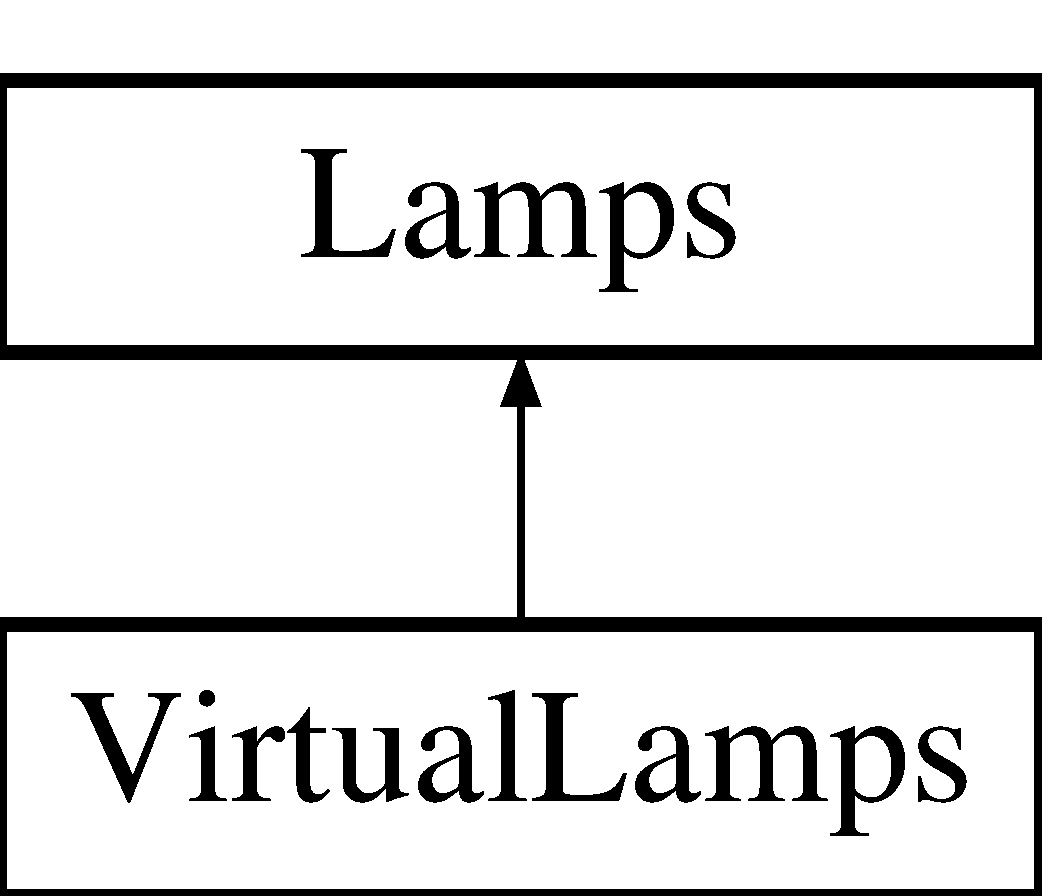
\includegraphics[height=2.000000cm]{classVirtualLamps}
\end{center}
\end{figure}
\subsubsection*{\-Public \-Member \-Functions}
\begin{DoxyCompactItemize}
\item 
\hyperlink{classVirtualLamps_affc72765153ab552943f9977de9d0322}{\-Virtual\-Lamps} (int \hyperlink{classLamps_a64146e584dfa86281df86a37dd7cb772}{num\-Lamps})
\item 
\hyperlink{classVirtualLamps_a4341fd24507ab5d860baa894e960c26c}{$\sim$\-Virtual\-Lamps} ()
\item 
bool \hyperlink{classVirtualLamps_ad1e55b2045b9bf34bc085fc79f47ef90}{is\-Ready} ()
\item 
bool \hyperlink{classVirtualLamps_a0b1e1847c16c5283ad95c29f9142bbc9}{send} ()
\end{DoxyCompactItemize}


\subsubsection{\-Detailed \-Description}
\hyperlink{classLamps}{\-Lamps} w/o hardware backend. 

\subsubsection{\-Constructor \& \-Destructor \-Documentation}
\hypertarget{classVirtualLamps_affc72765153ab552943f9977de9d0322}{\index{\-Virtual\-Lamps@{\-Virtual\-Lamps}!\-Virtual\-Lamps@{\-Virtual\-Lamps}}
\index{\-Virtual\-Lamps@{\-Virtual\-Lamps}!VirtualLamps@{\-Virtual\-Lamps}}
\paragraph[{\-Virtual\-Lamps}]{\setlength{\rightskip}{0pt plus 5cm}{\bf \-Virtual\-Lamps\-::\-Virtual\-Lamps} (
\begin{DoxyParamCaption}
\item[{int}]{num\-Lamps}
\end{DoxyParamCaption}
)}}\label{classVirtualLamps_affc72765153ab552943f9977de9d0322}
\begin{DoxyAuthor}{\-Author}
\-Manuel \-Jerger $<$\href{mailto:nom@nomnom.de}{\tt nom@nomnom.\-de}$>$
\end{DoxyAuthor}
\-This class represents a group of virtual monochrome lamps \hypertarget{classVirtualLamps_a4341fd24507ab5d860baa894e960c26c}{\index{\-Virtual\-Lamps@{\-Virtual\-Lamps}!$\sim$\-Virtual\-Lamps@{$\sim$\-Virtual\-Lamps}}
\index{$\sim$\-Virtual\-Lamps@{$\sim$\-Virtual\-Lamps}!VirtualLamps@{\-Virtual\-Lamps}}
\paragraph[{$\sim$\-Virtual\-Lamps}]{\setlength{\rightskip}{0pt plus 5cm}{\bf \-Virtual\-Lamps\-::$\sim$\-Virtual\-Lamps} (
\begin{DoxyParamCaption}
{}
\end{DoxyParamCaption}
)\hspace{0.3cm}{\ttfamily  \mbox{[}inline\mbox{]}}}}\label{classVirtualLamps_a4341fd24507ab5d860baa894e960c26c}


\subsubsection{\-Member \-Function \-Documentation}
\hypertarget{classVirtualLamps_ad1e55b2045b9bf34bc085fc79f47ef90}{\index{\-Virtual\-Lamps@{\-Virtual\-Lamps}!is\-Ready@{is\-Ready}}
\index{is\-Ready@{is\-Ready}!VirtualLamps@{\-Virtual\-Lamps}}
\paragraph[{is\-Ready}]{\setlength{\rightskip}{0pt plus 5cm}bool {\bf \-Virtual\-Lamps\-::is\-Ready} (
\begin{DoxyParamCaption}
{}
\end{DoxyParamCaption}
)\hspace{0.3cm}{\ttfamily  \mbox{[}virtual\mbox{]}}}}\label{classVirtualLamps_ad1e55b2045b9bf34bc085fc79f47ef90}


\-Implements \hyperlink{classLamps_aad615bf90ffa5f5d52d409a354a1942a}{\-Lamps}.

\hypertarget{classVirtualLamps_a0b1e1847c16c5283ad95c29f9142bbc9}{\index{\-Virtual\-Lamps@{\-Virtual\-Lamps}!send@{send}}
\index{send@{send}!VirtualLamps@{\-Virtual\-Lamps}}
\paragraph[{send}]{\setlength{\rightskip}{0pt plus 5cm}bool {\bf \-Virtual\-Lamps\-::send} (
\begin{DoxyParamCaption}
{}
\end{DoxyParamCaption}
)\hspace{0.3cm}{\ttfamily  \mbox{[}virtual\mbox{]}}}}\label{classVirtualLamps_a0b1e1847c16c5283ad95c29f9142bbc9}


\-Implements \hyperlink{classLamps_a9e5db6658a005b574d6344dab747bf4a}{\-Lamps}.



\-The documentation for this class was generated from the following files\-:\begin{DoxyCompactItemize}
\item 
src/\hyperlink{virtuallamps_8h}{virtuallamps.\-h}\item 
src/\hyperlink{virtuallamps_8cpp}{virtuallamps.\-cpp}\end{DoxyCompactItemize}

\hypertarget{classX11Source}{\subsection{\-X11\-Source \-Class \-Reference}
\label{classX11Source}\index{\-X11\-Source@{\-X11\-Source}}
}


\-X11 desktop grabber.  




{\ttfamily \#include $<$x11source.\-h$>$}

\-Inheritance diagram for \-X11\-Source\-:\begin{figure}[H]
\begin{center}
\leavevmode
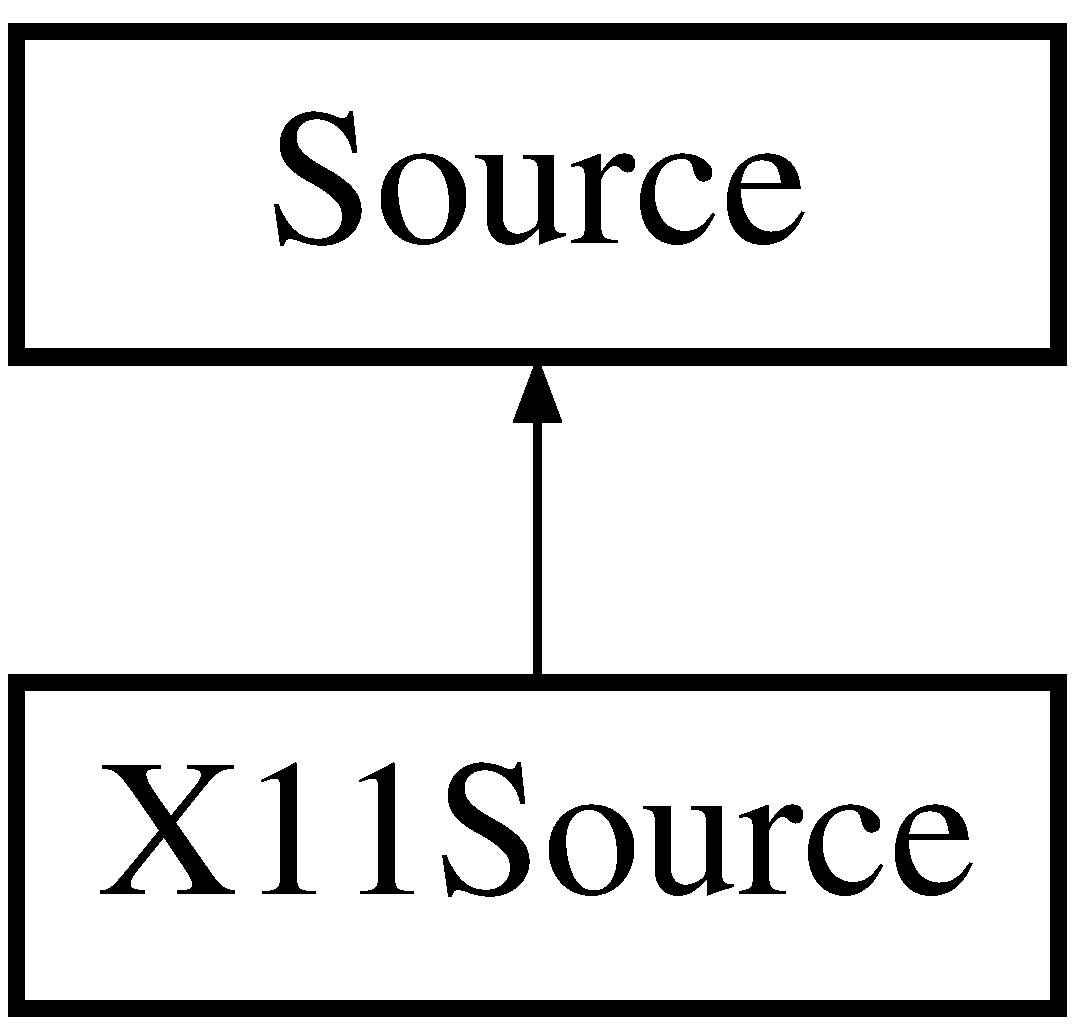
\includegraphics[height=2.000000cm]{classX11Source}
\end{center}
\end{figure}
\subsubsection*{\-Data \-Structures}
\begin{DoxyCompactItemize}
\item 
struct \hyperlink{structX11Source_1_1params}{params}
\begin{DoxyCompactList}\small\item\em \-Configuration of \hyperlink{classX11Source}{\-X11\-Source}. \end{DoxyCompactList}\end{DoxyCompactItemize}
\subsubsection*{\-Public \-Member \-Functions}
\begin{DoxyCompactItemize}
\item 
\hyperlink{classX11Source_a78acc272509b4489ba63e31708f15679}{\-X11\-Source} (\hyperlink{structX11Source_1_1params}{params} c)
\item 
\hyperlink{classX11Source_ac84c868de1b1ad71165dda3426cd03b3}{\-X11\-Source} (string \hyperlink{classX11Source_aca767875225424e06a91240ce66878fd}{display}, \hyperlink{structrect}{rect} area, double rate)
\item 
\hyperlink{classX11Source_a40ce038f2f6099f2ade3a07ebbfa1ddf}{$\sim$\-X11\-Source} ()
\item 
\hyperlink{structX11Source_1_1params}{params} \hyperlink{classX11Source_a7463cf93c1a347420ea423c993fb3db0}{get\-Config} ()
\item 
void \hyperlink{classX11Source_a1f1e97d8c02bfe6d5d84fb06a06125ba}{acquire} ()
\item 
bool \hyperlink{classX11Source_aa9b91f2a4a6db72b9391bc43d8f73944}{has\-New\-Data} ()
\item 
char $\ast$ \hyperlink{classX11Source_a224081f6ba7b80a1f4606cad8887e190}{get\-Image\-Raw} ()
\item 
const \hyperlink{structrect}{rect} \hyperlink{classX11Source_afcec9428c2cc28dca81f6839d079ca0f}{x11\-Select\-Area\-On\-Desktop} (string \hyperlink{classX11Source_aca767875225424e06a91240ce66878fd}{display})
\item 
const \hyperlink{structpoint}{point} \hyperlink{classX11Source_a8664f8ad4c33f46437cc2f02a5b76e49}{x11\-Select\-Point\-On\-Desktop} (\-Display $\ast$disp)
\end{DoxyCompactItemize}
\subsubsection*{\-Private \-Member \-Functions}
\begin{DoxyCompactItemize}
\item 
void \hyperlink{classX11Source_a44750861c3d995fae7436aff4940f372}{init} ()
\end{DoxyCompactItemize}
\subsubsection*{\-Private \-Attributes}
\begin{DoxyCompactItemize}
\item 
\hyperlink{structX11Source_1_1params}{params} \hyperlink{classX11Source_a0bb66f8a67eaf9fd1a9c7cd457744e6a}{config}
\item 
string \hyperlink{classX11Source_aca767875225424e06a91240ce66878fd}{display}
\item 
\-Display $\ast$ \hyperlink{classX11Source_ab29ca4f07bd4d6e512d900268b9ae6e4}{dpy}
\item 
\-X\-Shm\-Segment\-Info \hyperlink{classX11Source_a77384d75a89d1fdd0cb3f20f61453f46}{shminfo}
\item 
\-X\-Image $\ast$ \hyperlink{classX11Source_a88bec28d12299ca93f4516a1e6ce7cff}{x\-Image}
\end{DoxyCompactItemize}


\subsubsection{\-Detailed \-Description}
\-X11 desktop grabber. 

\begin{DoxyAuthor}{\-Author}
\-Manuel \-Jerger $<$\href{mailto:nom@nomnom.de}{\tt nom@nomnom.\-de}$>$
\end{DoxyAuthor}
\-Specialization of the source class that grabs images from the \-X11 desktop. 

\subsubsection{\-Constructor \& \-Destructor \-Documentation}
\hypertarget{classX11Source_a78acc272509b4489ba63e31708f15679}{\index{\-X11\-Source@{\-X11\-Source}!\-X11\-Source@{\-X11\-Source}}
\index{\-X11\-Source@{\-X11\-Source}!X11Source@{\-X11\-Source}}
\paragraph[{\-X11\-Source}]{\setlength{\rightskip}{0pt plus 5cm}{\bf \-X11\-Source\-::\-X11\-Source} (
\begin{DoxyParamCaption}
\item[{{\bf params}}]{c}
\end{DoxyParamCaption}
)}}\label{classX11Source_a78acc272509b4489ba63e31708f15679}
\hypertarget{classX11Source_ac84c868de1b1ad71165dda3426cd03b3}{\index{\-X11\-Source@{\-X11\-Source}!\-X11\-Source@{\-X11\-Source}}
\index{\-X11\-Source@{\-X11\-Source}!X11Source@{\-X11\-Source}}
\paragraph[{\-X11\-Source}]{\setlength{\rightskip}{0pt plus 5cm}{\bf \-X11\-Source\-::\-X11\-Source} (
\begin{DoxyParamCaption}
\item[{string}]{display, }
\item[{{\bf rect}}]{area, }
\item[{double}]{rate}
\end{DoxyParamCaption}
)}}\label{classX11Source_ac84c868de1b1ad71165dda3426cd03b3}
\hypertarget{classX11Source_a40ce038f2f6099f2ade3a07ebbfa1ddf}{\index{\-X11\-Source@{\-X11\-Source}!$\sim$\-X11\-Source@{$\sim$\-X11\-Source}}
\index{$\sim$\-X11\-Source@{$\sim$\-X11\-Source}!X11Source@{\-X11\-Source}}
\paragraph[{$\sim$\-X11\-Source}]{\setlength{\rightskip}{0pt plus 5cm}{\bf \-X11\-Source\-::$\sim$\-X11\-Source} (
\begin{DoxyParamCaption}
{}
\end{DoxyParamCaption}
)}}\label{classX11Source_a40ce038f2f6099f2ade3a07ebbfa1ddf}


\subsubsection{\-Member \-Function \-Documentation}
\hypertarget{classX11Source_a1f1e97d8c02bfe6d5d84fb06a06125ba}{\index{\-X11\-Source@{\-X11\-Source}!acquire@{acquire}}
\index{acquire@{acquire}!X11Source@{\-X11\-Source}}
\paragraph[{acquire}]{\setlength{\rightskip}{0pt plus 5cm}void {\bf \-X11\-Source\-::acquire} (
\begin{DoxyParamCaption}
{}
\end{DoxyParamCaption}
)\hspace{0.3cm}{\ttfamily  \mbox{[}virtual\mbox{]}}}}\label{classX11Source_a1f1e97d8c02bfe6d5d84fb06a06125ba}
\-Grabs one image from desktop 

\-Implements \hyperlink{classSource_a22e791e3c667fe6d65fa79b30ddc44da}{\-Source}.

\hypertarget{classX11Source_a7463cf93c1a347420ea423c993fb3db0}{\index{\-X11\-Source@{\-X11\-Source}!get\-Config@{get\-Config}}
\index{get\-Config@{get\-Config}!X11Source@{\-X11\-Source}}
\paragraph[{get\-Config}]{\setlength{\rightskip}{0pt plus 5cm}{\bf \-X11\-Source\-::params} {\bf \-X11\-Source\-::get\-Config} (
\begin{DoxyParamCaption}
{}
\end{DoxyParamCaption}
)}}\label{classX11Source_a7463cf93c1a347420ea423c993fb3db0}
\hypertarget{classX11Source_a224081f6ba7b80a1f4606cad8887e190}{\index{\-X11\-Source@{\-X11\-Source}!get\-Image\-Raw@{get\-Image\-Raw}}
\index{get\-Image\-Raw@{get\-Image\-Raw}!X11Source@{\-X11\-Source}}
\paragraph[{get\-Image\-Raw}]{\setlength{\rightskip}{0pt plus 5cm}char $\ast$ {\bf \-X11\-Source\-::get\-Image\-Raw} (
\begin{DoxyParamCaption}
{}
\end{DoxyParamCaption}
)}}\label{classX11Source_a224081f6ba7b80a1f4606cad8887e190}
\-Returns image data straight from \-X11 shared memory. \hypertarget{classX11Source_aa9b91f2a4a6db72b9391bc43d8f73944}{\index{\-X11\-Source@{\-X11\-Source}!has\-New\-Data@{has\-New\-Data}}
\index{has\-New\-Data@{has\-New\-Data}!X11Source@{\-X11\-Source}}
\paragraph[{has\-New\-Data}]{\setlength{\rightskip}{0pt plus 5cm}bool {\bf \-X11\-Source\-::has\-New\-Data} (
\begin{DoxyParamCaption}
{}
\end{DoxyParamCaption}
)\hspace{0.3cm}{\ttfamily  \mbox{[}virtual\mbox{]}}}}\label{classX11Source_aa9b91f2a4a6db72b9391bc43d8f73944}


\-Implements \hyperlink{classSource_acc6f90436f56986b5d261c2408bc1196}{\-Source}.

\hypertarget{classX11Source_a44750861c3d995fae7436aff4940f372}{\index{\-X11\-Source@{\-X11\-Source}!init@{init}}
\index{init@{init}!X11Source@{\-X11\-Source}}
\paragraph[{init}]{\setlength{\rightskip}{0pt plus 5cm}void {\bf \-X11\-Source\-::init} (
\begin{DoxyParamCaption}
{}
\end{DoxyParamCaption}
)\hspace{0.3cm}{\ttfamily  \mbox{[}private\mbox{]}}}}\label{classX11Source_a44750861c3d995fae7436aff4940f372}
\-Initialize \-X11 image grabbing. \hypertarget{classX11Source_afcec9428c2cc28dca81f6839d079ca0f}{\index{\-X11\-Source@{\-X11\-Source}!x11\-Select\-Area\-On\-Desktop@{x11\-Select\-Area\-On\-Desktop}}
\index{x11\-Select\-Area\-On\-Desktop@{x11\-Select\-Area\-On\-Desktop}!X11Source@{\-X11\-Source}}
\paragraph[{x11\-Select\-Area\-On\-Desktop}]{\setlength{\rightskip}{0pt plus 5cm}const {\bf rect} {\bf \-X11\-Source\-::x11\-Select\-Area\-On\-Desktop} (
\begin{DoxyParamCaption}
\item[{string}]{display}
\end{DoxyParamCaption}
)}}\label{classX11Source_afcec9428c2cc28dca81f6839d079ca0f}
\-Asks the user to select two points on the desktop that define the top left and bottom right corner of the image area to grab. \hypertarget{classX11Source_a8664f8ad4c33f46437cc2f02a5b76e49}{\index{\-X11\-Source@{\-X11\-Source}!x11\-Select\-Point\-On\-Desktop@{x11\-Select\-Point\-On\-Desktop}}
\index{x11\-Select\-Point\-On\-Desktop@{x11\-Select\-Point\-On\-Desktop}!X11Source@{\-X11\-Source}}
\paragraph[{x11\-Select\-Point\-On\-Desktop}]{\setlength{\rightskip}{0pt plus 5cm}const {\bf point} {\bf \-X11\-Source\-::x11\-Select\-Point\-On\-Desktop} (
\begin{DoxyParamCaption}
\item[{\-Display $\ast$}]{disp}
\end{DoxyParamCaption}
)}}\label{classX11Source_a8664f8ad4c33f46437cc2f02a5b76e49}
\-Asks the user to select a points on the desktop. \-Uses \-X11 functions for displaying a cursor and reacting to the click. 

\subsubsection{\-Field \-Documentation}
\hypertarget{classX11Source_a0bb66f8a67eaf9fd1a9c7cd457744e6a}{\index{\-X11\-Source@{\-X11\-Source}!config@{config}}
\index{config@{config}!X11Source@{\-X11\-Source}}
\paragraph[{config}]{\setlength{\rightskip}{0pt plus 5cm}{\bf params} {\bf \-X11\-Source\-::config}\hspace{0.3cm}{\ttfamily  \mbox{[}private\mbox{]}}}}\label{classX11Source_a0bb66f8a67eaf9fd1a9c7cd457744e6a}
\hypertarget{classX11Source_aca767875225424e06a91240ce66878fd}{\index{\-X11\-Source@{\-X11\-Source}!display@{display}}
\index{display@{display}!X11Source@{\-X11\-Source}}
\paragraph[{display}]{\setlength{\rightskip}{0pt plus 5cm}string {\bf \-X11\-Source\-::display}\hspace{0.3cm}{\ttfamily  \mbox{[}private\mbox{]}}}}\label{classX11Source_aca767875225424e06a91240ce66878fd}
\hypertarget{classX11Source_ab29ca4f07bd4d6e512d900268b9ae6e4}{\index{\-X11\-Source@{\-X11\-Source}!dpy@{dpy}}
\index{dpy@{dpy}!X11Source@{\-X11\-Source}}
\paragraph[{dpy}]{\setlength{\rightskip}{0pt plus 5cm}\-Display$\ast$ {\bf \-X11\-Source\-::dpy}\hspace{0.3cm}{\ttfamily  \mbox{[}private\mbox{]}}}}\label{classX11Source_ab29ca4f07bd4d6e512d900268b9ae6e4}
\hypertarget{classX11Source_a77384d75a89d1fdd0cb3f20f61453f46}{\index{\-X11\-Source@{\-X11\-Source}!shminfo@{shminfo}}
\index{shminfo@{shminfo}!X11Source@{\-X11\-Source}}
\paragraph[{shminfo}]{\setlength{\rightskip}{0pt plus 5cm}\-X\-Shm\-Segment\-Info {\bf \-X11\-Source\-::shminfo}\hspace{0.3cm}{\ttfamily  \mbox{[}private\mbox{]}}}}\label{classX11Source_a77384d75a89d1fdd0cb3f20f61453f46}
\hypertarget{classX11Source_a88bec28d12299ca93f4516a1e6ce7cff}{\index{\-X11\-Source@{\-X11\-Source}!x\-Image@{x\-Image}}
\index{x\-Image@{x\-Image}!X11Source@{\-X11\-Source}}
\paragraph[{x\-Image}]{\setlength{\rightskip}{0pt plus 5cm}\-X\-Image$\ast$ {\bf \-X11\-Source\-::x\-Image}\hspace{0.3cm}{\ttfamily  \mbox{[}private\mbox{]}}}}\label{classX11Source_a88bec28d12299ca93f4516a1e6ce7cff}


\-The documentation for this class was generated from the following files\-:\begin{DoxyCompactItemize}
\item 
src/\hyperlink{x11source_8h}{x11source.\-h}\item 
src/\hyperlink{x11source_8cpp}{x11source.\-cpp}\end{DoxyCompactItemize}

\hypertarget{structX11Source_1_1params}{\subsection{\-X11\-Source\-:\-:params \-Struct \-Reference}
\label{structX11Source_1_1params}\index{\-X11\-Source\-::params@{\-X11\-Source\-::params}}
}


\-Configuration of \hyperlink{classX11Source}{\-X11\-Source}.  




{\ttfamily \#include $<$x11source.\-h$>$}

\subsubsection*{\-Public \-Member \-Functions}
\begin{DoxyCompactItemize}
\item 
\hyperlink{structX11Source_1_1params_ae121992de8279b62254df5e3730980d3}{params} ()
\end{DoxyCompactItemize}
\subsubsection*{\-Data \-Fields}
\begin{DoxyCompactItemize}
\item 
string \hyperlink{structX11Source_1_1params_a04dd0457d0564d0a53898ae0d12b3950}{x11\-Display}
\item 
\hyperlink{structrect}{rect} \hyperlink{structX11Source_1_1params_adc58aad60a470f9e40ba4a8092e0d9d5}{capture\-Area}
\item 
double \hyperlink{structX11Source_1_1params_a218cb1cd1a5d80372fcb4bfe0ec1917b}{update\-Rate}
\end{DoxyCompactItemize}


\subsubsection{\-Detailed \-Description}
\-Configuration of \hyperlink{classX11Source}{\-X11\-Source}. 

\subsubsection{\-Constructor \& \-Destructor \-Documentation}
\hypertarget{structX11Source_1_1params_ae121992de8279b62254df5e3730980d3}{\index{\-X11\-Source\-::params@{\-X11\-Source\-::params}!params@{params}}
\index{params@{params}!X11Source::params@{\-X11\-Source\-::params}}
\paragraph[{params}]{\setlength{\rightskip}{0pt plus 5cm}{\bf \-X11\-Source\-::params\-::params} (
\begin{DoxyParamCaption}
{}
\end{DoxyParamCaption}
)\hspace{0.3cm}{\ttfamily  \mbox{[}inline\mbox{]}}}}\label{structX11Source_1_1params_ae121992de8279b62254df5e3730980d3}


\subsubsection{\-Field \-Documentation}
\hypertarget{structX11Source_1_1params_adc58aad60a470f9e40ba4a8092e0d9d5}{\index{\-X11\-Source\-::params@{\-X11\-Source\-::params}!capture\-Area@{capture\-Area}}
\index{capture\-Area@{capture\-Area}!X11Source::params@{\-X11\-Source\-::params}}
\paragraph[{capture\-Area}]{\setlength{\rightskip}{0pt plus 5cm}{\bf rect} {\bf \-X11\-Source\-::params\-::capture\-Area}}}\label{structX11Source_1_1params_adc58aad60a470f9e40ba4a8092e0d9d5}
\hypertarget{structX11Source_1_1params_a218cb1cd1a5d80372fcb4bfe0ec1917b}{\index{\-X11\-Source\-::params@{\-X11\-Source\-::params}!update\-Rate@{update\-Rate}}
\index{update\-Rate@{update\-Rate}!X11Source::params@{\-X11\-Source\-::params}}
\paragraph[{update\-Rate}]{\setlength{\rightskip}{0pt plus 5cm}double {\bf \-X11\-Source\-::params\-::update\-Rate}}}\label{structX11Source_1_1params_a218cb1cd1a5d80372fcb4bfe0ec1917b}
\hypertarget{structX11Source_1_1params_a04dd0457d0564d0a53898ae0d12b3950}{\index{\-X11\-Source\-::params@{\-X11\-Source\-::params}!x11\-Display@{x11\-Display}}
\index{x11\-Display@{x11\-Display}!X11Source::params@{\-X11\-Source\-::params}}
\paragraph[{x11\-Display}]{\setlength{\rightskip}{0pt plus 5cm}string {\bf \-X11\-Source\-::params\-::x11\-Display}}}\label{structX11Source_1_1params_a04dd0457d0564d0a53898ae0d12b3950}


\-The documentation for this struct was generated from the following file\-:\begin{DoxyCompactItemize}
\item 
src/\hyperlink{x11source_8h}{x11source.\-h}\end{DoxyCompactItemize}

\section{\-File \-Documentation}
\hypertarget{alt_8cpp}{\subsection{src/alt.cpp \-File \-Reference}
\label{alt_8cpp}\index{src/alt.\-cpp@{src/alt.\-cpp}}
}
{\ttfamily \#include \char`\"{}alt.\-h\char`\"{}}\*
\subsubsection*{\-Functions}
\begin{DoxyCompactItemize}
\item 
void \hyperlink{alt_8cpp_a6984903d33c27d46af404c6cfcf48c96}{parse\-Args} (int argc, char $\ast$argv\mbox{[}$\,$\mbox{]})
\item 
void \hyperlink{alt_8cpp_abac2c035abaf9d7d0ed5d5334a4cc030}{segfault\-Handler} (int sig)
\item 
int \hyperlink{alt_8cpp_a0ddf1224851353fc92bfbff6f499fa97}{main} (int argc, char $\ast$argv\mbox{[}$\,$\mbox{]})
\end{DoxyCompactItemize}
\subsubsection*{\-Variables}
\begin{DoxyCompactItemize}
\item 
int \hyperlink{alt_8cpp_aa1b60b2ca03f9253582ee6ba9dd7fe8c}{progmode} = \hyperlink{alt_8h_a06fc87d81c62e9abb8790b6e5713c55bac1bee29cc4915cda4b613b8b95330663}{\-T\-R\-A\-N\-S\-F\-E\-R}
\item 
int \hyperlink{alt_8cpp_af0c3b60f26d2028618ce9a8918a22b0c}{master\-Arg} = 0
\item 
int \hyperlink{alt_8cpp_a1bdcfae3209cbd96db35a2ae356fa15e}{verbosity}
\item 
\hyperlink{structCalibrate_1_1params}{\-Calibrate\-::params} \hyperlink{alt_8cpp_a2eb6a43d9c5165888a627ae5f8814b44}{cali\-Config}
\item 
\hyperlink{structTransfer_1_1params}{\-Transfer\-::params} \hyperlink{alt_8cpp_a2423264b3b11d7436df7b8812596c608}{transfer\-Config}
\item 
\hyperlink{structSticks_1_1params}{\-Sticks\-::params} \hyperlink{alt_8cpp_a4374a22f277d38c77345c2c3535accb4}{sticks\-Config}
\item 
\hyperlink{structX11Source_1_1params}{\-X11\-Source\-::params} \hyperlink{alt_8cpp_a4beade74199bf5fee501b5dc80ed5296}{x11source\-Config}
\item 
\hyperlink{structImageSource_1_1params}{\-Image\-Source\-::params} \hyperlink{alt_8cpp_ae9b191d559645fa6fe52f5727d1deda1}{imagesource\-Config}
\item 
\hyperlink{structLightprobe_1_1params}{\-Lightprobe\-::params} \hyperlink{alt_8cpp_a674145bab725b2746c177b7f1ca21f25}{probe\-Config}
\item 
\hyperlink{structLightprobe_1_1samplingParams}{\-Lightprobe\-::sampling\-Params} \hyperlink{alt_8cpp_a3e27d12a44b5e4ceeed4f9551f594ca4}{sampling\-Config}
\item 
vector$<$ pair$<$ int, double $>$ $>$ \hyperlink{alt_8cpp_a9035d443740b8416211400fcf1fa8940}{set\-Lamps\-Values}
\item 
\hyperlink{structrgb}{rgb} \hyperlink{alt_8cpp_aabf41615d4ff3039521228da4d27238d}{set\-Lamps\-R\-G\-B}
\item 
string \hyperlink{alt_8cpp_ab9343acb30f2a450c390c40bbc2bc103}{set\-Lamps\-File}
\item 
int \hyperlink{alt_8cpp_a971c348c530b233174e1a8e60b04b7ce}{num\-Virtual\-Lamps} = 0
\item 
bool \hyperlink{alt_8cpp_a733d993af149c761301e19aa50ac9979}{use\-Sticks} = false
\item 
int \hyperlink{alt_8cpp_a3c948b1e47a3a41e0688594113bc992b}{source\-Type}
\item 
bool \hyperlink{alt_8cpp_aec8a5664eabf09bcdfbe4861f9a22111}{probe\-Args} = false
\item 
bool \hyperlink{alt_8cpp_a5d2aa0deffd6c584c5d63e6b39595e0c}{stick\-Args} = false
\item 
static struct option \hyperlink{alt_8cpp_a450cc7e6593d545e2aa83bdab1bde867}{long\-Options} \mbox{[}$\,$\mbox{]}
\end{DoxyCompactItemize}


\subsubsection{\-Function \-Documentation}
\hypertarget{alt_8cpp_a0ddf1224851353fc92bfbff6f499fa97}{\index{alt.\-cpp@{alt.\-cpp}!main@{main}}
\index{main@{main}!alt.cpp@{alt.\-cpp}}
\paragraph[{main}]{\setlength{\rightskip}{0pt plus 5cm}int {\bf main} (
\begin{DoxyParamCaption}
\item[{int}]{argc, }
\item[{char $\ast$}]{argv\mbox{[}$\,$\mbox{]}}
\end{DoxyParamCaption}
)}}\label{alt_8cpp_a0ddf1224851353fc92bfbff6f499fa97}
\-Program entry point.

\-Main() parses the command line arguments and sets up all our classes using the specified configurations. \-It then runs the specified program mode.


\begin{DoxyParams}{\-Parameters}
{\em argc} & \-Number of arguments. \\
\hline
{\em argv} & \-Arguments \\
\hline
\end{DoxyParams}
\hypertarget{alt_8cpp_a6984903d33c27d46af404c6cfcf48c96}{\index{alt.\-cpp@{alt.\-cpp}!parse\-Args@{parse\-Args}}
\index{parse\-Args@{parse\-Args}!alt.cpp@{alt.\-cpp}}
\paragraph[{parse\-Args}]{\setlength{\rightskip}{0pt plus 5cm}void {\bf parse\-Args} (
\begin{DoxyParamCaption}
\item[{int}]{argc, }
\item[{char $\ast$}]{argv\mbox{[}$\,$\mbox{]}}
\end{DoxyParamCaption}
)}}\label{alt_8cpp_a6984903d33c27d46af404c6cfcf48c96}
\-Parse command line arguments and set the program configuration accordingly.


\begin{DoxyParams}{\-Parameters}
{\em argc} & \-Forwarded argc from \hyperlink{alt_8cpp_a0ddf1224851353fc92bfbff6f499fa97}{main()} \\
\hline
{\em argv} & \-Forwarded argv from \hyperlink{alt_8cpp_a0ddf1224851353fc92bfbff6f499fa97}{main()} \\
\hline
\end{DoxyParams}
\hypertarget{alt_8cpp_abac2c035abaf9d7d0ed5d5334a4cc030}{\index{alt.\-cpp@{alt.\-cpp}!segfault\-Handler@{segfault\-Handler}}
\index{segfault\-Handler@{segfault\-Handler}!alt.cpp@{alt.\-cpp}}
\paragraph[{segfault\-Handler}]{\setlength{\rightskip}{0pt plus 5cm}void {\bf segfault\-Handler} (
\begin{DoxyParamCaption}
\item[{int}]{sig}
\end{DoxyParamCaption}
)}}\label{alt_8cpp_abac2c035abaf9d7d0ed5d5334a4cc030}
\-Add segfault handler and print a backtrace using backtrace() (a feature available in gcc)


\begin{DoxyParams}{\-Parameters}
{\em sig} & signal number \\
\hline
\end{DoxyParams}


\subsubsection{\-Variable \-Documentation}
\hypertarget{alt_8cpp_a2eb6a43d9c5165888a627ae5f8814b44}{\index{alt.\-cpp@{alt.\-cpp}!cali\-Config@{cali\-Config}}
\index{cali\-Config@{cali\-Config}!alt.cpp@{alt.\-cpp}}
\paragraph[{cali\-Config}]{\setlength{\rightskip}{0pt plus 5cm}{\bf \-Calibrate\-::params} {\bf cali\-Config}}}\label{alt_8cpp_a2eb6a43d9c5165888a627ae5f8814b44}
\hypertarget{alt_8cpp_ae9b191d559645fa6fe52f5727d1deda1}{\index{alt.\-cpp@{alt.\-cpp}!imagesource\-Config@{imagesource\-Config}}
\index{imagesource\-Config@{imagesource\-Config}!alt.cpp@{alt.\-cpp}}
\paragraph[{imagesource\-Config}]{\setlength{\rightskip}{0pt plus 5cm}{\bf \-Image\-Source\-::params} {\bf imagesource\-Config}}}\label{alt_8cpp_ae9b191d559645fa6fe52f5727d1deda1}
\hypertarget{alt_8cpp_a450cc7e6593d545e2aa83bdab1bde867}{\index{alt.\-cpp@{alt.\-cpp}!long\-Options@{long\-Options}}
\index{long\-Options@{long\-Options}!alt.cpp@{alt.\-cpp}}
\paragraph[{long\-Options}]{\setlength{\rightskip}{0pt plus 5cm}struct option {\bf long\-Options}\mbox{[}$\,$\mbox{]}\hspace{0.3cm}{\ttfamily  \mbox{[}static\mbox{]}}}}\label{alt_8cpp_a450cc7e6593d545e2aa83bdab1bde867}
\hypertarget{alt_8cpp_af0c3b60f26d2028618ce9a8918a22b0c}{\index{alt.\-cpp@{alt.\-cpp}!master\-Arg@{master\-Arg}}
\index{master\-Arg@{master\-Arg}!alt.cpp@{alt.\-cpp}}
\paragraph[{master\-Arg}]{\setlength{\rightskip}{0pt plus 5cm}int {\bf master\-Arg} = 0}}\label{alt_8cpp_af0c3b60f26d2028618ce9a8918a22b0c}
\hypertarget{alt_8cpp_a971c348c530b233174e1a8e60b04b7ce}{\index{alt.\-cpp@{alt.\-cpp}!num\-Virtual\-Lamps@{num\-Virtual\-Lamps}}
\index{num\-Virtual\-Lamps@{num\-Virtual\-Lamps}!alt.cpp@{alt.\-cpp}}
\paragraph[{num\-Virtual\-Lamps}]{\setlength{\rightskip}{0pt plus 5cm}int {\bf num\-Virtual\-Lamps} = 0}}\label{alt_8cpp_a971c348c530b233174e1a8e60b04b7ce}
\hypertarget{alt_8cpp_aec8a5664eabf09bcdfbe4861f9a22111}{\index{alt.\-cpp@{alt.\-cpp}!probe\-Args@{probe\-Args}}
\index{probe\-Args@{probe\-Args}!alt.cpp@{alt.\-cpp}}
\paragraph[{probe\-Args}]{\setlength{\rightskip}{0pt plus 5cm}bool {\bf probe\-Args} = false}}\label{alt_8cpp_aec8a5664eabf09bcdfbe4861f9a22111}
\hypertarget{alt_8cpp_a674145bab725b2746c177b7f1ca21f25}{\index{alt.\-cpp@{alt.\-cpp}!probe\-Config@{probe\-Config}}
\index{probe\-Config@{probe\-Config}!alt.cpp@{alt.\-cpp}}
\paragraph[{probe\-Config}]{\setlength{\rightskip}{0pt plus 5cm}{\bf \-Lightprobe\-::params} {\bf probe\-Config}}}\label{alt_8cpp_a674145bab725b2746c177b7f1ca21f25}
\hypertarget{alt_8cpp_aa1b60b2ca03f9253582ee6ba9dd7fe8c}{\index{alt.\-cpp@{alt.\-cpp}!progmode@{progmode}}
\index{progmode@{progmode}!alt.cpp@{alt.\-cpp}}
\paragraph[{progmode}]{\setlength{\rightskip}{0pt plus 5cm}int {\bf progmode} = {\bf \-T\-R\-A\-N\-S\-F\-E\-R}}}\label{alt_8cpp_aa1b60b2ca03f9253582ee6ba9dd7fe8c}
\hypertarget{alt_8cpp_a3e27d12a44b5e4ceeed4f9551f594ca4}{\index{alt.\-cpp@{alt.\-cpp}!sampling\-Config@{sampling\-Config}}
\index{sampling\-Config@{sampling\-Config}!alt.cpp@{alt.\-cpp}}
\paragraph[{sampling\-Config}]{\setlength{\rightskip}{0pt plus 5cm}{\bf \-Lightprobe\-::sampling\-Params} {\bf sampling\-Config}}}\label{alt_8cpp_a3e27d12a44b5e4ceeed4f9551f594ca4}
\hypertarget{alt_8cpp_ab9343acb30f2a450c390c40bbc2bc103}{\index{alt.\-cpp@{alt.\-cpp}!set\-Lamps\-File@{set\-Lamps\-File}}
\index{set\-Lamps\-File@{set\-Lamps\-File}!alt.cpp@{alt.\-cpp}}
\paragraph[{set\-Lamps\-File}]{\setlength{\rightskip}{0pt plus 5cm}string {\bf set\-Lamps\-File}}}\label{alt_8cpp_ab9343acb30f2a450c390c40bbc2bc103}
\hypertarget{alt_8cpp_aabf41615d4ff3039521228da4d27238d}{\index{alt.\-cpp@{alt.\-cpp}!set\-Lamps\-R\-G\-B@{set\-Lamps\-R\-G\-B}}
\index{set\-Lamps\-R\-G\-B@{set\-Lamps\-R\-G\-B}!alt.cpp@{alt.\-cpp}}
\paragraph[{set\-Lamps\-R\-G\-B}]{\setlength{\rightskip}{0pt plus 5cm}{\bf rgb} {\bf set\-Lamps\-R\-G\-B}}}\label{alt_8cpp_aabf41615d4ff3039521228da4d27238d}
\hypertarget{alt_8cpp_a9035d443740b8416211400fcf1fa8940}{\index{alt.\-cpp@{alt.\-cpp}!set\-Lamps\-Values@{set\-Lamps\-Values}}
\index{set\-Lamps\-Values@{set\-Lamps\-Values}!alt.cpp@{alt.\-cpp}}
\paragraph[{set\-Lamps\-Values}]{\setlength{\rightskip}{0pt plus 5cm}vector$<$pair$<$int, double$>$ $>$ {\bf set\-Lamps\-Values}}}\label{alt_8cpp_a9035d443740b8416211400fcf1fa8940}
\hypertarget{alt_8cpp_a3c948b1e47a3a41e0688594113bc992b}{\index{alt.\-cpp@{alt.\-cpp}!source\-Type@{source\-Type}}
\index{source\-Type@{source\-Type}!alt.cpp@{alt.\-cpp}}
\paragraph[{source\-Type}]{\setlength{\rightskip}{0pt plus 5cm}int {\bf source\-Type}}}\label{alt_8cpp_a3c948b1e47a3a41e0688594113bc992b}
\hypertarget{alt_8cpp_a5d2aa0deffd6c584c5d63e6b39595e0c}{\index{alt.\-cpp@{alt.\-cpp}!stick\-Args@{stick\-Args}}
\index{stick\-Args@{stick\-Args}!alt.cpp@{alt.\-cpp}}
\paragraph[{stick\-Args}]{\setlength{\rightskip}{0pt plus 5cm}bool {\bf stick\-Args} = false}}\label{alt_8cpp_a5d2aa0deffd6c584c5d63e6b39595e0c}
\hypertarget{alt_8cpp_a4374a22f277d38c77345c2c3535accb4}{\index{alt.\-cpp@{alt.\-cpp}!sticks\-Config@{sticks\-Config}}
\index{sticks\-Config@{sticks\-Config}!alt.cpp@{alt.\-cpp}}
\paragraph[{sticks\-Config}]{\setlength{\rightskip}{0pt plus 5cm}{\bf \-Sticks\-::params} {\bf sticks\-Config}}}\label{alt_8cpp_a4374a22f277d38c77345c2c3535accb4}
\hypertarget{alt_8cpp_a2423264b3b11d7436df7b8812596c608}{\index{alt.\-cpp@{alt.\-cpp}!transfer\-Config@{transfer\-Config}}
\index{transfer\-Config@{transfer\-Config}!alt.cpp@{alt.\-cpp}}
\paragraph[{transfer\-Config}]{\setlength{\rightskip}{0pt plus 5cm}{\bf \-Transfer\-::params} {\bf transfer\-Config}}}\label{alt_8cpp_a2423264b3b11d7436df7b8812596c608}
\hypertarget{alt_8cpp_a733d993af149c761301e19aa50ac9979}{\index{alt.\-cpp@{alt.\-cpp}!use\-Sticks@{use\-Sticks}}
\index{use\-Sticks@{use\-Sticks}!alt.cpp@{alt.\-cpp}}
\paragraph[{use\-Sticks}]{\setlength{\rightskip}{0pt plus 5cm}bool {\bf use\-Sticks} = false}}\label{alt_8cpp_a733d993af149c761301e19aa50ac9979}
\hypertarget{alt_8cpp_a1bdcfae3209cbd96db35a2ae356fa15e}{\index{alt.\-cpp@{alt.\-cpp}!verbosity@{verbosity}}
\index{verbosity@{verbosity}!alt.cpp@{alt.\-cpp}}
\paragraph[{verbosity}]{\setlength{\rightskip}{0pt plus 5cm}int {\bf verbosity}}}\label{alt_8cpp_a1bdcfae3209cbd96db35a2ae356fa15e}
\begin{DoxyAuthor}{\-Author}
\-Manuel \-Jerger $<$\href{mailto:nom@nomnom.de}{\tt nom@nomnom.\-de}$>$
\end{DoxyAuthor}
\-Utility functions and important datastructures. \hypertarget{alt_8cpp_a4beade74199bf5fee501b5dc80ed5296}{\index{alt.\-cpp@{alt.\-cpp}!x11source\-Config@{x11source\-Config}}
\index{x11source\-Config@{x11source\-Config}!alt.cpp@{alt.\-cpp}}
\paragraph[{x11source\-Config}]{\setlength{\rightskip}{0pt plus 5cm}{\bf \-X11\-Source\-::params} {\bf x11source\-Config}}}\label{alt_8cpp_a4beade74199bf5fee501b5dc80ed5296}

\hypertarget{alt_8h}{\subsection{src/alt.h \-File \-Reference}
\label{alt_8h}\index{src/alt.\-h@{src/alt.\-h}}
}
{\ttfamily \#include \char`\"{}utils.\-h\char`\"{}}\*
{\ttfamily \#include \char`\"{}gui.\-h\char`\"{}}\*
{\ttfamily \#include \char`\"{}lamps.\-h\char`\"{}}\*
{\ttfamily \#include \char`\"{}lamppool.\-h\char`\"{}}\*
{\ttfamily \#include \char`\"{}virtuallamps.\-h\char`\"{}}\*
{\ttfamily \#include \char`\"{}sticks.\-h\char`\"{}}\*
{\ttfamily \#include \char`\"{}x11source.\-h\char`\"{}}\*
{\ttfamily \#include \char`\"{}lightprobe.\-h\char`\"{}}\*
{\ttfamily \#include \char`\"{}transfer.\-h\char`\"{}}\*
{\ttfamily \#include \char`\"{}calibrate.\-h\char`\"{}}\*
{\ttfamily \#include \char`\"{}testlamps.\-h\char`\"{}}\*
{\ttfamily \#include \char`\"{}testprobe.\-h\char`\"{}}\*
{\ttfamily \#include \char`\"{}maxexposure.\-h\char`\"{}}\*
{\ttfamily \#include \char`\"{}sandbox.\-h\char`\"{}}\*
{\ttfamily \#include $<$iostream$>$}\*
{\ttfamily \#include $<$sstream$>$}\*
{\ttfamily \#include $<$stdio.\-h$>$}\*
{\ttfamily \#include $<$string.\-h$>$}\*
{\ttfamily \#include $<$vector$>$}\*
{\ttfamily \#include $<$\-Eigen/\-Core$>$}\*
{\ttfamily \#include $<$\-Eigen/\-Geometry$>$}\*
{\ttfamily \#include $<$getopt.\-h$>$}\*
{\ttfamily \#include $<$\-X11/\-Xlib.\-h$>$}\*
{\ttfamily \#include $<$execinfo.\-h$>$}\*
{\ttfamily \#include $<$signal.\-h$>$}\*
\subsubsection*{\-Enumerations}
\begin{DoxyCompactItemize}
\item 
enum \{ \*
\hyperlink{alt_8h_a06fc87d81c62e9abb8790b6e5713c55bac1bee29cc4915cda4b613b8b95330663}{\-T\-R\-A\-N\-S\-F\-E\-R}, 
\hyperlink{alt_8h_a06fc87d81c62e9abb8790b6e5713c55ba54fd7b44442a8ea505e7a21822838a06}{\-T\-R\-A\-N\-S\-F\-E\-R\-\_\-\-S\-A\-M\-P\-L\-E\-R}, 
\hyperlink{alt_8h_a06fc87d81c62e9abb8790b6e5713c55ba2a90047fe45c6934034c89fd9fb5dbbb}{\-C\-A\-P\-T\-U\-R\-E}, 
\hyperlink{alt_8h_a06fc87d81c62e9abb8790b6e5713c55ba167eb3a1a129f780224e29afaf7c5dc0}{\-C\-A\-L\-I\-B\-R\-A\-T\-E\-\_\-\-L\-A\-M\-P\-S}, 
\*
\hyperlink{alt_8h_a06fc87d81c62e9abb8790b6e5713c55bae4a2d127a60de705b4d68ce65a77c76a}{\-T\-E\-S\-T\-L\-A\-M\-P\-S}, 
\hyperlink{alt_8h_a06fc87d81c62e9abb8790b6e5713c55ba244b8da74ee286cbce5638a6d0534396}{\-T\-E\-S\-T\-P\-R\-O\-B\-E}, 
\hyperlink{alt_8h_a06fc87d81c62e9abb8790b6e5713c55badfde72dcb3e83861ae0ce5fa19869c67}{\-S\-E\-T\-L\-A\-M\-P\-S}, 
\hyperlink{alt_8h_a06fc87d81c62e9abb8790b6e5713c55ba5aa58c66842151fcd531abffc34ba5ce}{\-M\-A\-X\-\_\-\-E\-X\-P\-O\-S\-U\-R\-E}, 
\*
\hyperlink{alt_8h_a06fc87d81c62e9abb8790b6e5713c55baaea380afb93100c32477ab63fc0fef05}{\-S\-A\-N\-D\-B\-O\-X}, 
\hyperlink{alt_8h_a06fc87d81c62e9abb8790b6e5713c55ba5d8b4dc32c8c0ce55b3a5eef3a9d9356}{\-S\-A\-M\-P\-L\-E\-\_\-\-U\-N\-I\-\_\-\-O\-L\-D}, 
\hyperlink{alt_8h_a06fc87d81c62e9abb8790b6e5713c55ba2decb46d0aee4a025934a88b17d3a49f}{\-S\-A\-M\-P\-L\-E\-\_\-\-U\-N\-I}, 
\hyperlink{alt_8h_a06fc87d81c62e9abb8790b6e5713c55ba0aa8ca6cfcd46da32a6085b86737389e}{\-S\-A\-M\-P\-L\-E\-\_\-\-F\-I\-L\-E}, 
\*
\hyperlink{alt_8h_a06fc87d81c62e9abb8790b6e5713c55ba656ae9228add5538f7320103ed9508eb}{\-S\-A\-M\-P\-L\-E\-\_\-\-A\-L\-L}, 
\hyperlink{alt_8h_a06fc87d81c62e9abb8790b6e5713c55ba7b66109ea96919447e3f3ab34a83c0b4}{\-X11\-S\-O\-U\-R\-C\-E}, 
\hyperlink{alt_8h_a06fc87d81c62e9abb8790b6e5713c55ba887e118d33b5b30aa581f1e545d52577}{\-I\-M\-A\-G\-E\-S\-O\-U\-R\-C\-E}, 
\hyperlink{alt_8h_a06fc87d81c62e9abb8790b6e5713c55bacff66cd07ed61c173483181160dea538}{\-S\-T\-I\-C\-K\-S}, 
\*
\hyperlink{alt_8h_a06fc87d81c62e9abb8790b6e5713c55ba0f82b220d3986705f12947a4c783c2a9}{\-V\-I\-R\-T\-U\-A\-L\-\_\-\-L\-A\-M\-P\-S}, 
\hyperlink{alt_8h_a06fc87d81c62e9abb8790b6e5713c55ba0ad70b39c10fc8f55a84f2f88573d1b1}{\-L\-I\-G\-H\-T\-P\-R\-O\-B\-E}
 \}
\end{DoxyCompactItemize}


\subsubsection{\-Enumeration \-Type \-Documentation}
\hypertarget{alt_8h_a06fc87d81c62e9abb8790b6e5713c55b}{\paragraph[{anonymous enum}]{\setlength{\rightskip}{0pt plus 5cm}anonymous enum}}\label{alt_8h_a06fc87d81c62e9abb8790b6e5713c55b}
\begin{Desc}
\item[\-Enumerator\-: ]\par
\begin{description}
\index{\-T\-R\-A\-N\-S\-F\-E\-R@{\-T\-R\-A\-N\-S\-F\-E\-R}!alt.\-h@{alt.\-h}}\index{alt.\-h@{alt.\-h}!\-T\-R\-A\-N\-S\-F\-E\-R@{\-T\-R\-A\-N\-S\-F\-E\-R}}\item[{\em 
\hypertarget{alt_8h_a06fc87d81c62e9abb8790b6e5713c55bac1bee29cc4915cda4b613b8b95330663}{\-T\-R\-A\-N\-S\-F\-E\-R}\label{alt_8h_a06fc87d81c62e9abb8790b6e5713c55bac1bee29cc4915cda4b613b8b95330663}
}]\index{\-T\-R\-A\-N\-S\-F\-E\-R\-\_\-\-S\-A\-M\-P\-L\-E\-R@{\-T\-R\-A\-N\-S\-F\-E\-R\-\_\-\-S\-A\-M\-P\-L\-E\-R}!alt.\-h@{alt.\-h}}\index{alt.\-h@{alt.\-h}!\-T\-R\-A\-N\-S\-F\-E\-R\-\_\-\-S\-A\-M\-P\-L\-E\-R@{\-T\-R\-A\-N\-S\-F\-E\-R\-\_\-\-S\-A\-M\-P\-L\-E\-R}}\item[{\em 
\hypertarget{alt_8h_a06fc87d81c62e9abb8790b6e5713c55ba54fd7b44442a8ea505e7a21822838a06}{\-T\-R\-A\-N\-S\-F\-E\-R\-\_\-\-S\-A\-M\-P\-L\-E\-R}\label{alt_8h_a06fc87d81c62e9abb8790b6e5713c55ba54fd7b44442a8ea505e7a21822838a06}
}]\index{\-C\-A\-P\-T\-U\-R\-E@{\-C\-A\-P\-T\-U\-R\-E}!alt.\-h@{alt.\-h}}\index{alt.\-h@{alt.\-h}!\-C\-A\-P\-T\-U\-R\-E@{\-C\-A\-P\-T\-U\-R\-E}}\item[{\em 
\hypertarget{alt_8h_a06fc87d81c62e9abb8790b6e5713c55ba2a90047fe45c6934034c89fd9fb5dbbb}{\-C\-A\-P\-T\-U\-R\-E}\label{alt_8h_a06fc87d81c62e9abb8790b6e5713c55ba2a90047fe45c6934034c89fd9fb5dbbb}
}]\index{\-C\-A\-L\-I\-B\-R\-A\-T\-E\-\_\-\-L\-A\-M\-P\-S@{\-C\-A\-L\-I\-B\-R\-A\-T\-E\-\_\-\-L\-A\-M\-P\-S}!alt.\-h@{alt.\-h}}\index{alt.\-h@{alt.\-h}!\-C\-A\-L\-I\-B\-R\-A\-T\-E\-\_\-\-L\-A\-M\-P\-S@{\-C\-A\-L\-I\-B\-R\-A\-T\-E\-\_\-\-L\-A\-M\-P\-S}}\item[{\em 
\hypertarget{alt_8h_a06fc87d81c62e9abb8790b6e5713c55ba167eb3a1a129f780224e29afaf7c5dc0}{\-C\-A\-L\-I\-B\-R\-A\-T\-E\-\_\-\-L\-A\-M\-P\-S}\label{alt_8h_a06fc87d81c62e9abb8790b6e5713c55ba167eb3a1a129f780224e29afaf7c5dc0}
}]\index{\-T\-E\-S\-T\-L\-A\-M\-P\-S@{\-T\-E\-S\-T\-L\-A\-M\-P\-S}!alt.\-h@{alt.\-h}}\index{alt.\-h@{alt.\-h}!\-T\-E\-S\-T\-L\-A\-M\-P\-S@{\-T\-E\-S\-T\-L\-A\-M\-P\-S}}\item[{\em 
\hypertarget{alt_8h_a06fc87d81c62e9abb8790b6e5713c55bae4a2d127a60de705b4d68ce65a77c76a}{\-T\-E\-S\-T\-L\-A\-M\-P\-S}\label{alt_8h_a06fc87d81c62e9abb8790b6e5713c55bae4a2d127a60de705b4d68ce65a77c76a}
}]\index{\-T\-E\-S\-T\-P\-R\-O\-B\-E@{\-T\-E\-S\-T\-P\-R\-O\-B\-E}!alt.\-h@{alt.\-h}}\index{alt.\-h@{alt.\-h}!\-T\-E\-S\-T\-P\-R\-O\-B\-E@{\-T\-E\-S\-T\-P\-R\-O\-B\-E}}\item[{\em 
\hypertarget{alt_8h_a06fc87d81c62e9abb8790b6e5713c55ba244b8da74ee286cbce5638a6d0534396}{\-T\-E\-S\-T\-P\-R\-O\-B\-E}\label{alt_8h_a06fc87d81c62e9abb8790b6e5713c55ba244b8da74ee286cbce5638a6d0534396}
}]\index{\-S\-E\-T\-L\-A\-M\-P\-S@{\-S\-E\-T\-L\-A\-M\-P\-S}!alt.\-h@{alt.\-h}}\index{alt.\-h@{alt.\-h}!\-S\-E\-T\-L\-A\-M\-P\-S@{\-S\-E\-T\-L\-A\-M\-P\-S}}\item[{\em 
\hypertarget{alt_8h_a06fc87d81c62e9abb8790b6e5713c55badfde72dcb3e83861ae0ce5fa19869c67}{\-S\-E\-T\-L\-A\-M\-P\-S}\label{alt_8h_a06fc87d81c62e9abb8790b6e5713c55badfde72dcb3e83861ae0ce5fa19869c67}
}]\index{\-M\-A\-X\-\_\-\-E\-X\-P\-O\-S\-U\-R\-E@{\-M\-A\-X\-\_\-\-E\-X\-P\-O\-S\-U\-R\-E}!alt.\-h@{alt.\-h}}\index{alt.\-h@{alt.\-h}!\-M\-A\-X\-\_\-\-E\-X\-P\-O\-S\-U\-R\-E@{\-M\-A\-X\-\_\-\-E\-X\-P\-O\-S\-U\-R\-E}}\item[{\em 
\hypertarget{alt_8h_a06fc87d81c62e9abb8790b6e5713c55ba5aa58c66842151fcd531abffc34ba5ce}{\-M\-A\-X\-\_\-\-E\-X\-P\-O\-S\-U\-R\-E}\label{alt_8h_a06fc87d81c62e9abb8790b6e5713c55ba5aa58c66842151fcd531abffc34ba5ce}
}]\index{\-S\-A\-N\-D\-B\-O\-X@{\-S\-A\-N\-D\-B\-O\-X}!alt.\-h@{alt.\-h}}\index{alt.\-h@{alt.\-h}!\-S\-A\-N\-D\-B\-O\-X@{\-S\-A\-N\-D\-B\-O\-X}}\item[{\em 
\hypertarget{alt_8h_a06fc87d81c62e9abb8790b6e5713c55baaea380afb93100c32477ab63fc0fef05}{\-S\-A\-N\-D\-B\-O\-X}\label{alt_8h_a06fc87d81c62e9abb8790b6e5713c55baaea380afb93100c32477ab63fc0fef05}
}]\index{\-S\-A\-M\-P\-L\-E\-\_\-\-U\-N\-I\-\_\-\-O\-L\-D@{\-S\-A\-M\-P\-L\-E\-\_\-\-U\-N\-I\-\_\-\-O\-L\-D}!alt.\-h@{alt.\-h}}\index{alt.\-h@{alt.\-h}!\-S\-A\-M\-P\-L\-E\-\_\-\-U\-N\-I\-\_\-\-O\-L\-D@{\-S\-A\-M\-P\-L\-E\-\_\-\-U\-N\-I\-\_\-\-O\-L\-D}}\item[{\em 
\hypertarget{alt_8h_a06fc87d81c62e9abb8790b6e5713c55ba5d8b4dc32c8c0ce55b3a5eef3a9d9356}{\-S\-A\-M\-P\-L\-E\-\_\-\-U\-N\-I\-\_\-\-O\-L\-D}\label{alt_8h_a06fc87d81c62e9abb8790b6e5713c55ba5d8b4dc32c8c0ce55b3a5eef3a9d9356}
}]\index{\-S\-A\-M\-P\-L\-E\-\_\-\-U\-N\-I@{\-S\-A\-M\-P\-L\-E\-\_\-\-U\-N\-I}!alt.\-h@{alt.\-h}}\index{alt.\-h@{alt.\-h}!\-S\-A\-M\-P\-L\-E\-\_\-\-U\-N\-I@{\-S\-A\-M\-P\-L\-E\-\_\-\-U\-N\-I}}\item[{\em 
\hypertarget{alt_8h_a06fc87d81c62e9abb8790b6e5713c55ba2decb46d0aee4a025934a88b17d3a49f}{\-S\-A\-M\-P\-L\-E\-\_\-\-U\-N\-I}\label{alt_8h_a06fc87d81c62e9abb8790b6e5713c55ba2decb46d0aee4a025934a88b17d3a49f}
}]\index{\-S\-A\-M\-P\-L\-E\-\_\-\-F\-I\-L\-E@{\-S\-A\-M\-P\-L\-E\-\_\-\-F\-I\-L\-E}!alt.\-h@{alt.\-h}}\index{alt.\-h@{alt.\-h}!\-S\-A\-M\-P\-L\-E\-\_\-\-F\-I\-L\-E@{\-S\-A\-M\-P\-L\-E\-\_\-\-F\-I\-L\-E}}\item[{\em 
\hypertarget{alt_8h_a06fc87d81c62e9abb8790b6e5713c55ba0aa8ca6cfcd46da32a6085b86737389e}{\-S\-A\-M\-P\-L\-E\-\_\-\-F\-I\-L\-E}\label{alt_8h_a06fc87d81c62e9abb8790b6e5713c55ba0aa8ca6cfcd46da32a6085b86737389e}
}]\index{\-S\-A\-M\-P\-L\-E\-\_\-\-A\-L\-L@{\-S\-A\-M\-P\-L\-E\-\_\-\-A\-L\-L}!alt.\-h@{alt.\-h}}\index{alt.\-h@{alt.\-h}!\-S\-A\-M\-P\-L\-E\-\_\-\-A\-L\-L@{\-S\-A\-M\-P\-L\-E\-\_\-\-A\-L\-L}}\item[{\em 
\hypertarget{alt_8h_a06fc87d81c62e9abb8790b6e5713c55ba656ae9228add5538f7320103ed9508eb}{\-S\-A\-M\-P\-L\-E\-\_\-\-A\-L\-L}\label{alt_8h_a06fc87d81c62e9abb8790b6e5713c55ba656ae9228add5538f7320103ed9508eb}
}]\index{\-X11\-S\-O\-U\-R\-C\-E@{\-X11\-S\-O\-U\-R\-C\-E}!alt.\-h@{alt.\-h}}\index{alt.\-h@{alt.\-h}!\-X11\-S\-O\-U\-R\-C\-E@{\-X11\-S\-O\-U\-R\-C\-E}}\item[{\em 
\hypertarget{alt_8h_a06fc87d81c62e9abb8790b6e5713c55ba7b66109ea96919447e3f3ab34a83c0b4}{\-X11\-S\-O\-U\-R\-C\-E}\label{alt_8h_a06fc87d81c62e9abb8790b6e5713c55ba7b66109ea96919447e3f3ab34a83c0b4}
}]\index{\-I\-M\-A\-G\-E\-S\-O\-U\-R\-C\-E@{\-I\-M\-A\-G\-E\-S\-O\-U\-R\-C\-E}!alt.\-h@{alt.\-h}}\index{alt.\-h@{alt.\-h}!\-I\-M\-A\-G\-E\-S\-O\-U\-R\-C\-E@{\-I\-M\-A\-G\-E\-S\-O\-U\-R\-C\-E}}\item[{\em 
\hypertarget{alt_8h_a06fc87d81c62e9abb8790b6e5713c55ba887e118d33b5b30aa581f1e545d52577}{\-I\-M\-A\-G\-E\-S\-O\-U\-R\-C\-E}\label{alt_8h_a06fc87d81c62e9abb8790b6e5713c55ba887e118d33b5b30aa581f1e545d52577}
}]\index{\-S\-T\-I\-C\-K\-S@{\-S\-T\-I\-C\-K\-S}!alt.\-h@{alt.\-h}}\index{alt.\-h@{alt.\-h}!\-S\-T\-I\-C\-K\-S@{\-S\-T\-I\-C\-K\-S}}\item[{\em 
\hypertarget{alt_8h_a06fc87d81c62e9abb8790b6e5713c55bacff66cd07ed61c173483181160dea538}{\-S\-T\-I\-C\-K\-S}\label{alt_8h_a06fc87d81c62e9abb8790b6e5713c55bacff66cd07ed61c173483181160dea538}
}]\index{\-V\-I\-R\-T\-U\-A\-L\-\_\-\-L\-A\-M\-P\-S@{\-V\-I\-R\-T\-U\-A\-L\-\_\-\-L\-A\-M\-P\-S}!alt.\-h@{alt.\-h}}\index{alt.\-h@{alt.\-h}!\-V\-I\-R\-T\-U\-A\-L\-\_\-\-L\-A\-M\-P\-S@{\-V\-I\-R\-T\-U\-A\-L\-\_\-\-L\-A\-M\-P\-S}}\item[{\em 
\hypertarget{alt_8h_a06fc87d81c62e9abb8790b6e5713c55ba0f82b220d3986705f12947a4c783c2a9}{\-V\-I\-R\-T\-U\-A\-L\-\_\-\-L\-A\-M\-P\-S}\label{alt_8h_a06fc87d81c62e9abb8790b6e5713c55ba0f82b220d3986705f12947a4c783c2a9}
}]\index{\-L\-I\-G\-H\-T\-P\-R\-O\-B\-E@{\-L\-I\-G\-H\-T\-P\-R\-O\-B\-E}!alt.\-h@{alt.\-h}}\index{alt.\-h@{alt.\-h}!\-L\-I\-G\-H\-T\-P\-R\-O\-B\-E@{\-L\-I\-G\-H\-T\-P\-R\-O\-B\-E}}\item[{\em 
\hypertarget{alt_8h_a06fc87d81c62e9abb8790b6e5713c55ba0ad70b39c10fc8f55a84f2f88573d1b1}{\-L\-I\-G\-H\-T\-P\-R\-O\-B\-E}\label{alt_8h_a06fc87d81c62e9abb8790b6e5713c55ba0ad70b39c10fc8f55a84f2f88573d1b1}
}]\end{description}
\end{Desc}


\hypertarget{calibrate_8cpp}{\subsection{src/calibrate.cpp \-File \-Reference}
\label{calibrate_8cpp}\index{src/calibrate.\-cpp@{src/calibrate.\-cpp}}
}
{\ttfamily \#include \char`\"{}calibrate.\-h\char`\"{}}\*

\hypertarget{calibrate_8h}{\subsection{src/calibrate.h \-File \-Reference}
\label{calibrate_8h}\index{src/calibrate.\-h@{src/calibrate.\-h}}
}
{\ttfamily \#include \char`\"{}utils.\-h\char`\"{}}\*
{\ttfamily \#include \char`\"{}lamps.\-h\char`\"{}}\*
{\ttfamily \#include \char`\"{}lightprobe.\-h\char`\"{}}\*
{\ttfamily \#include \char`\"{}gui.\-h\char`\"{}}\*
{\ttfamily \#include \char`\"{}ceres/ceres.\-h\char`\"{}}\*
{\ttfamily \#include $<$glog/logging.\-h$>$}\*
\subsubsection*{\-Data \-Structures}
\begin{DoxyCompactItemize}
\item 
class \hyperlink{classCalibrate}{\-Calibrate}
\begin{DoxyCompactList}\small\item\em \-The \-Calibration \-Loop. \end{DoxyCompactList}\item 
struct \hyperlink{structCalibrate_1_1params}{\-Calibrate\-::params}
\begin{DoxyCompactList}\small\item\em \-Configuration of \hyperlink{classCalibrate}{\-Calibrate} class. \end{DoxyCompactList}\end{DoxyCompactItemize}

\hypertarget{gui_8cpp}{\subsection{src/gui.cpp \-File \-Reference}
\label{gui_8cpp}\index{src/gui.\-cpp@{src/gui.\-cpp}}
}
{\ttfamily \#include \char`\"{}gui.\-h\char`\"{}}\*

\hypertarget{gui_8h}{\subsection{src/gui.h \-File \-Reference}
\label{gui_8h}\index{src/gui.\-h@{src/gui.\-h}}
}
{\ttfamily \#include \char`\"{}utils.\-h\char`\"{}}\*
{\ttfamily \#include \char`\"{}lamps.\-h\char`\"{}}\*
{\ttfamily \#include \char`\"{}sticks.\-h\char`\"{}}\*
{\ttfamily \#include \char`\"{}image.\-h\char`\"{}}\*
{\ttfamily \#include \char`\"{}source.\-h\char`\"{}}\*
{\ttfamily \#include $<$unistd.\-h$>$}\*
{\ttfamily \#include \char`\"{}\-G\-L/glfw.\-h\char`\"{}}\*
{\ttfamily \#include $<$\-G\-L/glu.\-h$>$}\*
\subsubsection*{\-Data \-Structures}
\begin{DoxyCompactItemize}
\item 
class \hyperlink{classGui}{\-Gui}
\begin{DoxyCompactList}\small\item\em \-The user interface. \end{DoxyCompactList}\end{DoxyCompactItemize}

\hypertarget{imagesource_8cpp}{\subsection{src/imagesource.cpp \-File \-Reference}
\label{imagesource_8cpp}\index{src/imagesource.\-cpp@{src/imagesource.\-cpp}}
}
{\ttfamily \#include \char`\"{}imagesource.\-h\char`\"{}}\*

\hypertarget{imagesource_8h}{\subsection{src/imagesource.h \-File \-Reference}
\label{imagesource_8h}\index{src/imagesource.\-h@{src/imagesource.\-h}}
}
{\ttfamily \#include \char`\"{}source.\-h\char`\"{}}\*
{\ttfamily \#include \char`\"{}image.\-h\char`\"{}}\*
{\ttfamily \#include $<$string$>$}\*
\subsubsection*{\-Data \-Structures}
\begin{DoxyCompactItemize}
\item 
class \hyperlink{classImageSource}{\-Image\-Source}
\begin{DoxyCompactList}\small\item\em \hyperlink{classSource}{\-Source} that uses image files. \end{DoxyCompactList}\item 
struct \hyperlink{structImageSource_1_1params}{\-Image\-Source\-::params}
\begin{DoxyCompactList}\small\item\em \-Configuration of the \hyperlink{classImageSource}{\-Image\-Source} class. \end{DoxyCompactList}\end{DoxyCompactItemize}

\hypertarget{lamppool_8cpp}{\subsection{src/lamppool.cpp \-File \-Reference}
\label{lamppool_8cpp}\index{src/lamppool.\-cpp@{src/lamppool.\-cpp}}
}
{\ttfamily \#include \char`\"{}lamppool.\-h\char`\"{}}\*

\hypertarget{lamppool_8h}{\subsection{src/lamppool.h \-File \-Reference}
\label{lamppool_8h}\index{src/lamppool.\-h@{src/lamppool.\-h}}
}
{\ttfamily \#include \char`\"{}lamps.\-h\char`\"{}}\*
{\ttfamily \#include \char`\"{}utils.\-h\char`\"{}}\*
{\ttfamily \#include $<$string$>$}\*
{\ttfamily \#include $<$iostream$>$}\*
{\ttfamily \#include $<$vector$>$}\*
{\ttfamily \#include $<$pthread.\-h$>$}\*
{\ttfamily \#include $<$time.\-h$>$}\*
\subsubsection*{\-Data \-Structures}
\begin{DoxyCompactItemize}
\item 
class \hyperlink{classLampPool}{\-Lamp\-Pool}
\begin{DoxyCompactList}\small\item\em \-Groups instances of \hyperlink{classLamps}{\-Lamps}. \end{DoxyCompactList}\end{DoxyCompactItemize}

\hypertarget{lamps_8cpp}{\subsection{src/lamps.cpp \-File \-Reference}
\label{lamps_8cpp}\index{src/lamps.\-cpp@{src/lamps.\-cpp}}
}
{\ttfamily \#include \char`\"{}lamps.\-h\char`\"{}}\*

\hypertarget{lamps_8h}{\subsection{src/lamps.h \-File \-Reference}
\label{lamps_8h}\index{src/lamps.\-h@{src/lamps.\-h}}
}
{\ttfamily \#include \char`\"{}utils.\-h\char`\"{}}\*
{\ttfamily \#include $<$vector$>$}\*
\subsubsection*{\-Data \-Structures}
\begin{DoxyCompactItemize}
\item 
class \hyperlink{classLamps}{\-Lamps}
\begin{DoxyCompactList}\small\item\em \-A monochrome lamp. \end{DoxyCompactList}\end{DoxyCompactItemize}

\hypertarget{lightprobe_8cpp}{\subsection{src/lightprobe.cpp \-File \-Reference}
\label{lightprobe_8cpp}\index{src/lightprobe.\-cpp@{src/lightprobe.\-cpp}}
}
{\ttfamily \#include \char`\"{}lightprobe.\-h\char`\"{}}\*

\hypertarget{lightprobe_8h}{\subsection{src/lightprobe.h \-File \-Reference}
\label{lightprobe_8h}\index{src/lightprobe.\-h@{src/lightprobe.\-h}}
}
{\ttfamily \#include \char`\"{}utils.\-h\char`\"{}}\*
{\ttfamily \#include \char`\"{}source.\-h\char`\"{}}\*
{\ttfamily \#include \char`\"{}x11source.\-h\char`\"{}}\*
{\ttfamily \#include \char`\"{}imagesource.\-h\char`\"{}}\*
{\ttfamily \#include $<$iostream$>$}\*
{\ttfamily \#include $<$vector$>$}\*
{\ttfamily \#include $<$\-Eigen/\-Core$>$}\*
{\ttfamily \#include $<$\-Eigen/\-Geometry$>$}\*
\subsubsection*{\-Data \-Structures}
\begin{DoxyCompactItemize}
\item 
class \hyperlink{classLightprobe}{\-Lightprobe}
\begin{DoxyCompactList}\small\item\em \-Our light probe model. \end{DoxyCompactList}\item 
struct \hyperlink{structLightprobe_1_1params}{\-Lightprobe\-::params}
\begin{DoxyCompactList}\small\item\em \-Configuration of the light probe. \end{DoxyCompactList}\item 
struct \hyperlink{structLightprobe_1_1samplingParams}{\-Lightprobe\-::sampling\-Params}
\begin{DoxyCompactList}\small\item\em \-Configures sampling. \end{DoxyCompactList}\end{DoxyCompactItemize}

\hypertarget{maxexposure_8cpp}{\subsection{src/maxexposure.cpp \-File \-Reference}
\label{maxexposure_8cpp}\index{src/maxexposure.\-cpp@{src/maxexposure.\-cpp}}
}
{\ttfamily \#include \char`\"{}maxexposure.\-h\char`\"{}}\*

\hypertarget{maxexposure_8h}{\subsection{src/maxexposure.h \-File \-Reference}
\label{maxexposure_8h}\index{src/maxexposure.\-h@{src/maxexposure.\-h}}
}
{\ttfamily \#include \char`\"{}utils.\-h\char`\"{}}\*
{\ttfamily \#include \char`\"{}gui.\-h\char`\"{}}\*
{\ttfamily \#include \char`\"{}source.\-h\char`\"{}}\*
{\ttfamily \#include $<$unistd.\-h$>$}\*
\subsubsection*{\-Data \-Structures}
\begin{DoxyCompactItemize}
\item 
class \hyperlink{classMaxExposure}{\-Max\-Exposure}
\begin{DoxyCompactList}\small\item\em \-Adjusts the \-Exposure of a \-U\-V\-C webcam. \end{DoxyCompactList}\end{DoxyCompactItemize}

\hypertarget{sandbox_8cpp}{\subsection{src/sandbox.cpp \-File \-Reference}
\label{sandbox_8cpp}\index{src/sandbox.\-cpp@{src/sandbox.\-cpp}}
}
{\ttfamily \#include \char`\"{}sandbox.\-h\char`\"{}}\*

\hypertarget{sandbox_8h}{\subsection{src/sandbox.h \-File \-Reference}
\label{sandbox_8h}\index{src/sandbox.\-h@{src/sandbox.\-h}}
}
{\ttfamily \#include \char`\"{}utils.\-h\char`\"{}}\*
{\ttfamily \#include \char`\"{}gui.\-h\char`\"{}}\*
{\ttfamily \#include \char`\"{}source.\-h\char`\"{}}\*
{\ttfamily \#include \char`\"{}lightprobe.\-h\char`\"{}}\*
{\ttfamily \#include \char`\"{}lamps.\-h\char`\"{}}\*
{\ttfamily \#include $<$unistd.\-h$>$}\*
\subsubsection*{\-Data \-Structures}
\begin{DoxyCompactItemize}
\item 
class \hyperlink{classSandbox}{\-Sandbox}
\begin{DoxyCompactList}\small\item\em \-A sandbox for experiments. \end{DoxyCompactList}\end{DoxyCompactItemize}

\hypertarget{source_8cpp}{\subsection{src/source.cpp \-File \-Reference}
\label{source_8cpp}\index{src/source.\-cpp@{src/source.\-cpp}}
}
{\ttfamily \#include \char`\"{}source.\-h\char`\"{}}\*
\subsubsection*{\-Defines}
\begin{DoxyCompactItemize}
\item 
\#define \hyperlink{source_8cpp_a55f4ac00fe96dd70c9002bf4664ef5e5}{\-F\-L\-O\-O\-R\-\_\-\-N\-O\-I\-S\-E\-\_\-\-T\-H\-R\-E\-S\-H\-O\-L\-D}~(0.\-000)
\item 
\#define \hyperlink{source_8cpp_a427d1dc635214b6fa4da5cebe1e50dc3}{\-H\-I\-G\-H\-L\-I\-G\-H\-T\-\_\-\-T\-R\-E\-S\-H\-O\-L\-D}~(0.\-9)
\end{DoxyCompactItemize}


\subsubsection{\-Define \-Documentation}
\hypertarget{source_8cpp_a55f4ac00fe96dd70c9002bf4664ef5e5}{\index{source.\-cpp@{source.\-cpp}!\-F\-L\-O\-O\-R\-\_\-\-N\-O\-I\-S\-E\-\_\-\-T\-H\-R\-E\-S\-H\-O\-L\-D@{\-F\-L\-O\-O\-R\-\_\-\-N\-O\-I\-S\-E\-\_\-\-T\-H\-R\-E\-S\-H\-O\-L\-D}}
\index{\-F\-L\-O\-O\-R\-\_\-\-N\-O\-I\-S\-E\-\_\-\-T\-H\-R\-E\-S\-H\-O\-L\-D@{\-F\-L\-O\-O\-R\-\_\-\-N\-O\-I\-S\-E\-\_\-\-T\-H\-R\-E\-S\-H\-O\-L\-D}!source.cpp@{source.\-cpp}}
\paragraph[{\-F\-L\-O\-O\-R\-\_\-\-N\-O\-I\-S\-E\-\_\-\-T\-H\-R\-E\-S\-H\-O\-L\-D}]{\setlength{\rightskip}{0pt plus 5cm}\#define {\bf \-F\-L\-O\-O\-R\-\_\-\-N\-O\-I\-S\-E\-\_\-\-T\-H\-R\-E\-S\-H\-O\-L\-D}~(0.\-000)}}\label{source_8cpp_a55f4ac00fe96dd70c9002bf4664ef5e5}
\hypertarget{source_8cpp_a427d1dc635214b6fa4da5cebe1e50dc3}{\index{source.\-cpp@{source.\-cpp}!\-H\-I\-G\-H\-L\-I\-G\-H\-T\-\_\-\-T\-R\-E\-S\-H\-O\-L\-D@{\-H\-I\-G\-H\-L\-I\-G\-H\-T\-\_\-\-T\-R\-E\-S\-H\-O\-L\-D}}
\index{\-H\-I\-G\-H\-L\-I\-G\-H\-T\-\_\-\-T\-R\-E\-S\-H\-O\-L\-D@{\-H\-I\-G\-H\-L\-I\-G\-H\-T\-\_\-\-T\-R\-E\-S\-H\-O\-L\-D}!source.cpp@{source.\-cpp}}
\paragraph[{\-H\-I\-G\-H\-L\-I\-G\-H\-T\-\_\-\-T\-R\-E\-S\-H\-O\-L\-D}]{\setlength{\rightskip}{0pt plus 5cm}\#define {\bf \-H\-I\-G\-H\-L\-I\-G\-H\-T\-\_\-\-T\-R\-E\-S\-H\-O\-L\-D}~(0.\-9)}}\label{source_8cpp_a427d1dc635214b6fa4da5cebe1e50dc3}

\hypertarget{source_8h}{\subsection{src/source.h \-File \-Reference}
\label{source_8h}\index{src/source.\-h@{src/source.\-h}}
}
{\ttfamily \#include \char`\"{}utils.\-h\char`\"{}}\*
\subsubsection*{\-Data \-Structures}
\begin{DoxyCompactItemize}
\item 
class \hyperlink{classSource}{\-Source}
\begin{DoxyCompactList}\small\item\em \-Acquires and linearizes images. \end{DoxyCompactList}\end{DoxyCompactItemize}

\hypertarget{sticks_8cpp}{\subsection{src/sticks.cpp \-File \-Reference}
\label{sticks_8cpp}\index{src/sticks.\-cpp@{src/sticks.\-cpp}}
}
{\ttfamily \#include \char`\"{}sticks.\-h\char`\"{}}\*

\hypertarget{sticks_8h}{\subsection{src/sticks.h \-File \-Reference}
\label{sticks_8h}\index{src/sticks.\-h@{src/sticks.\-h}}
}
{\ttfamily \#include \char`\"{}lamps.\-h\char`\"{}}\*
{\ttfamily \#include \char`\"{}utils.\-h\char`\"{}}\*
{\ttfamily \#include $<$string$>$}\*
{\ttfamily \#include $<$iostream$>$}\*
{\ttfamily \#include $<$stdlib.\-h$>$}\*
{\ttfamily \#include $<$unistd.\-h$>$}\*
{\ttfamily \#include $<$fcntl.\-h$>$}\*
{\ttfamily \#include $<$errno.\-h$>$}\*
{\ttfamily \#include $<$termios.\-h$>$}\*
{\ttfamily \#include $<$vector$>$}\*
{\ttfamily \#include $<$pthread.\-h$>$}\*
{\ttfamily \#include $<$time.\-h$>$}\*
\subsubsection*{\-Data \-Structures}
\begin{DoxyCompactItemize}
\item 
class \hyperlink{classSticks}{\-Sticks}
\begin{DoxyCompactList}\small\item\em \-Our sticks lighting system. \end{DoxyCompactList}\item 
struct \hyperlink{structSticks_1_1params}{\-Sticks\-::params}
\begin{DoxyCompactList}\small\item\em \-Configuration of our lighting system. \end{DoxyCompactList}\end{DoxyCompactItemize}

\hypertarget{testlamps_8cpp}{\subsection{src/testlamps.cpp \-File \-Reference}
\label{testlamps_8cpp}\index{src/testlamps.\-cpp@{src/testlamps.\-cpp}}
}
{\ttfamily \#include \char`\"{}testlamps.\-h\char`\"{}}\*

\hypertarget{testlamps_8h}{\subsection{src/testlamps.h \-File \-Reference}
\label{testlamps_8h}\index{src/testlamps.\-h@{src/testlamps.\-h}}
}
{\ttfamily \#include \char`\"{}lamps.\-h\char`\"{}}\*
{\ttfamily \#include \char`\"{}source.\-h\char`\"{}}\*
{\ttfamily \#include \char`\"{}gui.\-h\char`\"{}}\*
\subsubsection*{\-Data \-Structures}
\begin{DoxyCompactItemize}
\item 
class \hyperlink{classTestLamps}{\-Test\-Lamps}
\begin{DoxyCompactList}\small\item\em \-Test lamps (for debug). \end{DoxyCompactList}\end{DoxyCompactItemize}

\hypertarget{testprobe_8cpp}{\subsection{src/testprobe.cpp \-File \-Reference}
\label{testprobe_8cpp}\index{src/testprobe.\-cpp@{src/testprobe.\-cpp}}
}
{\ttfamily \#include \char`\"{}testprobe.\-h\char`\"{}}\*

\hypertarget{testprobe_8h}{\subsection{src/testprobe.h \-File \-Reference}
\label{testprobe_8h}\index{src/testprobe.\-h@{src/testprobe.\-h}}
}
{\ttfamily \#include \char`\"{}lightprobe.\-h\char`\"{}}\*
{\ttfamily \#include \char`\"{}source.\-h\char`\"{}}\*
{\ttfamily \#include \char`\"{}gui.\-h\char`\"{}}\*
\subsubsection*{\-Data \-Structures}
\begin{DoxyCompactItemize}
\item 
class \hyperlink{classTestProbe}{\-Test\-Probe}
\begin{DoxyCompactList}\small\item\em \-Test light probe (for debug). \end{DoxyCompactList}\end{DoxyCompactItemize}

\hypertarget{transfer_8cpp}{\subsection{src/transfer.cpp \-File \-Reference}
\label{transfer_8cpp}\index{src/transfer.\-cpp@{src/transfer.\-cpp}}
}
{\ttfamily \#include \char`\"{}transfer.\-h\char`\"{}}\*
\subsubsection*{\-Defines}
\begin{DoxyCompactItemize}
\item 
\#define \hyperlink{transfer_8cpp_a8070e63641d964d89b5e7947bdfc9b1d}{\-M\-I\-N\-\_\-\-W\-E\-I\-G\-H\-T\-\_\-\-D\-I\-S\-T\-A\-N\-C\-E}~0.\-05
\end{DoxyCompactItemize}


\subsubsection{\-Define \-Documentation}
\hypertarget{transfer_8cpp_a8070e63641d964d89b5e7947bdfc9b1d}{\index{transfer.\-cpp@{transfer.\-cpp}!\-M\-I\-N\-\_\-\-W\-E\-I\-G\-H\-T\-\_\-\-D\-I\-S\-T\-A\-N\-C\-E@{\-M\-I\-N\-\_\-\-W\-E\-I\-G\-H\-T\-\_\-\-D\-I\-S\-T\-A\-N\-C\-E}}
\index{\-M\-I\-N\-\_\-\-W\-E\-I\-G\-H\-T\-\_\-\-D\-I\-S\-T\-A\-N\-C\-E@{\-M\-I\-N\-\_\-\-W\-E\-I\-G\-H\-T\-\_\-\-D\-I\-S\-T\-A\-N\-C\-E}!transfer.cpp@{transfer.\-cpp}}
\paragraph[{\-M\-I\-N\-\_\-\-W\-E\-I\-G\-H\-T\-\_\-\-D\-I\-S\-T\-A\-N\-C\-E}]{\setlength{\rightskip}{0pt plus 5cm}\#define {\bf \-M\-I\-N\-\_\-\-W\-E\-I\-G\-H\-T\-\_\-\-D\-I\-S\-T\-A\-N\-C\-E}~0.\-05}}\label{transfer_8cpp_a8070e63641d964d89b5e7947bdfc9b1d}

\hypertarget{transfer_8h}{\subsection{src/transfer.h \-File \-Reference}
\label{transfer_8h}\index{src/transfer.\-h@{src/transfer.\-h}}
}
{\ttfamily \#include \char`\"{}utils.\-h\char`\"{}}\*
{\ttfamily \#include \char`\"{}gui.\-h\char`\"{}}\*
{\ttfamily \#include \char`\"{}lamps.\-h\char`\"{}}\*
{\ttfamily \#include \char`\"{}lamppool.\-h\char`\"{}}\*
{\ttfamily \#include \char`\"{}virtuallamps.\-h\char`\"{}}\*
{\ttfamily \#include \char`\"{}source.\-h\char`\"{}}\*
{\ttfamily \#include \char`\"{}imagesource.\-h\char`\"{}}\*
{\ttfamily \#include \char`\"{}lightprobe.\-h\char`\"{}}\*
{\ttfamily \#include \char`\"{}image.\-h\char`\"{}}\*
{\ttfamily \#include $<$vector$>$}\*
{\ttfamily \#include $<$time.\-h$>$}\*
{\ttfamily \#include \char`\"{}\-G\-L/glfw.\-h\char`\"{}}\*
{\ttfamily \#include $<$\-G\-L/glu.\-h$>$}\*
{\ttfamily \#include $<$ceres/ceres.\-h$>$}\*
{\ttfamily \#include $<$glog/logging.\-h$>$}\*
{\ttfamily \#include \char`\"{}cvxopt.\-h\char`\"{}}\*
\subsubsection*{\-Data \-Structures}
\begin{DoxyCompactItemize}
\item 
class \hyperlink{classTransfer}{\-Transfer}
\begin{DoxyCompactList}\small\item\em \-The \-Ambient \-Light \hyperlink{classTransfer}{\-Transfer} loop. \end{DoxyCompactList}\item 
struct \hyperlink{structTransfer_1_1params}{\-Transfer\-::params}
\begin{DoxyCompactList}\small\item\em \-Configuration. \end{DoxyCompactList}\item 
struct \hyperlink{structTransfer_1_1Residual}{\-Transfer\-::\-Residual}
\begin{DoxyCompactList}\small\item\em \-Cost\-Function for ceres. \end{DoxyCompactList}\item 
class \hyperlink{classTransfer_1_1CostSimple}{\-Transfer\-::\-Cost\-Simple}
\begin{DoxyCompactList}\small\item\em \-Faster \-Cost\-Function for ceres. \end{DoxyCompactList}\end{DoxyCompactItemize}
\subsubsection*{\-Defines}
\begin{DoxyCompactItemize}
\item 
\#define \hyperlink{transfer_8h_ae27f1bdef26580f6409e2f4defdf1459}{\-P\-E\-N\-A\-L\-T\-Y}~100
\item 
\#define \hyperlink{transfer_8h_a9ae075a6945e35ed878e744202a1c173}{\-N\-U\-M\-L\-A\-M\-P\-S}~108
\end{DoxyCompactItemize}


\subsubsection{\-Define \-Documentation}
\hypertarget{transfer_8h_a9ae075a6945e35ed878e744202a1c173}{\index{transfer.\-h@{transfer.\-h}!\-N\-U\-M\-L\-A\-M\-P\-S@{\-N\-U\-M\-L\-A\-M\-P\-S}}
\index{\-N\-U\-M\-L\-A\-M\-P\-S@{\-N\-U\-M\-L\-A\-M\-P\-S}!transfer.h@{transfer.\-h}}
\paragraph[{\-N\-U\-M\-L\-A\-M\-P\-S}]{\setlength{\rightskip}{0pt plus 5cm}\#define {\bf \-N\-U\-M\-L\-A\-M\-P\-S}~108}}\label{transfer_8h_a9ae075a6945e35ed878e744202a1c173}
\hypertarget{transfer_8h_ae27f1bdef26580f6409e2f4defdf1459}{\index{transfer.\-h@{transfer.\-h}!\-P\-E\-N\-A\-L\-T\-Y@{\-P\-E\-N\-A\-L\-T\-Y}}
\index{\-P\-E\-N\-A\-L\-T\-Y@{\-P\-E\-N\-A\-L\-T\-Y}!transfer.h@{transfer.\-h}}
\paragraph[{\-P\-E\-N\-A\-L\-T\-Y}]{\setlength{\rightskip}{0pt plus 5cm}\#define {\bf \-P\-E\-N\-A\-L\-T\-Y}~100}}\label{transfer_8h_ae27f1bdef26580f6409e2f4defdf1459}

\hypertarget{utils_8cpp}{\subsection{src/utils.cpp \-File \-Reference}
\label{utils_8cpp}\index{src/utils.\-cpp@{src/utils.\-cpp}}
}
{\ttfamily \#include \char`\"{}utils.\-h\char`\"{}}\*
{\ttfamily \#include $<$getopt.\-h$>$}\*
\subsubsection*{\-Defines}
\begin{DoxyCompactItemize}
\item 
\#define \hyperlink{utils_8cpp_aea081df85db0cbf8310f4542db85a4cc}{\-M\-\_\-\-S\-Q\-R\-T2\-P\-I}~2.\-50662827463100050241
\end{DoxyCompactItemize}
\subsubsection*{\-Functions}
\begin{DoxyCompactItemize}
\item 
imglib\-::\-Image$<$ float $>$ \& \hyperlink{utils_8cpp_af70a156db2679c4f4c918393d5a013c6}{img\-Add} (imglib\-::\-Image$<$ float $>$ \&\-A, imglib\-::\-Image$<$ float $>$ \&\-B)
\item 
imglib\-::\-Image$<$ float $>$ \& \hyperlink{utils_8cpp_a7ba19ee1f4d56d1f4a6d98a6f620011e}{img\-Sub} (imglib\-::\-Image$<$ float $>$ \&\-A, imglib\-::\-Image$<$ float $>$ \&\-B)
\item 
imglib\-::\-Image$<$ float $>$ \& \hyperlink{utils_8cpp_af98ef3f5f3468c645f0a2106b50ac5bf}{img\-Add} (imglib\-::\-Image$<$ float $>$ \&\-A, \hyperlink{structrgb}{rgb} color)
\item 
imglib\-::\-Image$<$ float $>$ \& \hyperlink{utils_8cpp_a29c4f6b55dfafdcedeb7ebd7309716e4}{img\-Mul} (imglib\-::\-Image$<$ float $>$ \&\-A, float scalar)
\item 
float \hyperlink{utils_8cpp_ab3cf80dd119e5575fc54ebb1e41c36bd}{img\-Max} (imglib\-::\-Image$<$ float $>$ \&\-A)
\item 
float \hyperlink{utils_8cpp_a6d0a4da646579ef4f2ba1c2863873ef1}{img\-Min} (imglib\-::\-Image$<$ float $>$ \&\-A)
\item 
imglib\-::\-Image$<$ float $>$ \& \hyperlink{utils_8cpp_a55ba5b124ad940e5205aa63c646e1b36}{img\-Scale} (imglib\-::\-Image$<$ float $>$ \&\-A)
\item 
\hyperlink{structrgb}{rgb} \hyperlink{utils_8cpp_af055f18e7f3b08318ff949e6498ea0a9}{sample\-Gauss7} (imglib\-::\-Image$<$ float $>$ image, int xpos, int ypos)
\item 
double \hyperlink{utils_8cpp_a0dd39d56e3eda8d0ad575663bb0518bd}{normal\-Distribution} (double sigma, double mu, double x)
\item 
\hyperlink{structrgb}{rgb} \hyperlink{utils_8cpp_add8a5da556bccd6767b3b5b73625ff82}{map\-Gamma} (\hyperlink{structrgb}{rgb} value, double gain, double lambda)
\item 
double \hyperlink{utils_8cpp_acc3b81d5055f0e53011a09648d99cfd7}{map\-Linear} (double val, double wp, double bp)
\item 
\hyperlink{structrgb}{rgb} \hyperlink{utils_8cpp_aa07cc396e9f5909789bd7cd7585b4524}{map\-Linear} (\hyperlink{structrgb}{rgb} val, \hyperlink{structrgb}{rgb} wp, \hyperlink{structrgb}{rgb} bp)
\item 
\hyperlink{structrgb}{rgb} \hyperlink{utils_8cpp_aee4a0c84d71d303e5b0bfd9d45165cac}{rgb2srgb} (\hyperlink{structrgb}{rgb} linear)
\item 
double \hyperlink{utils_8cpp_a4b083da617f2c75fcc9420a725966d2d}{rgb2srgb\-\_\-component} (double value)
\item 
\-Vector3d \hyperlink{utils_8cpp_a5563c3ab02be36251e5f22d9ab41cd4b}{rgb2xy\-Y} (\hyperlink{structrgb}{rgb} val)
\item 
\hyperlink{structrgb}{rgb} \hyperlink{utils_8cpp_a0b4e2045baebfc2cec92224a94a06ab6}{srgb2rgb} (\hyperlink{structrgb}{rgb} s\-R\-G\-B)
\item 
double \hyperlink{utils_8cpp_a59ce04a4fb0e230afec6ba18357d019f}{srgb2rgb\-\_\-component} (double value)
\item 
double \hyperlink{utils_8cpp_ad97f7e15d40bc6ac70ec74122c8a38e3}{clamp} (double val)
\item 
\hyperlink{structrgb}{rgb} \hyperlink{utils_8cpp_a9f2c03a21b65ea931f510e959d9f3415}{clamp} (\hyperlink{structrgb}{rgb} val)
\item 
\hyperlink{structcircle}{circle} \hyperlink{utils_8cpp_acbb9d469878f84c33acaeae386ddfd9f}{get\-Circum\-Circle} (\-Vector2d p1, \-Vector2d p2, \-Vector2d p3)
\item 
\hyperlink{utils_8h_aac426d8086789d4d7e318436071c9754}{directions} \hyperlink{utils_8cpp_a0f01d4dd6fcb7ac2fc637cb0a23fb223}{sample\-Hemisphere} (int num\-Samples\-H, int num\-Samples\-A)
\item 
\hyperlink{utils_8h_aac426d8086789d4d7e318436071c9754}{directions} \hyperlink{utils_8cpp_a84f8b3bda17602bfef1e85642f09dfee}{sample\-Sphere} (int num\-Samples\-H, int num\-Samples\-A, double horizon\-Angle)
\item 
\hyperlink{utils_8h_aac426d8086789d4d7e318436071c9754}{directions} \hyperlink{utils_8cpp_a0599be5dae7949307a0cd655c91a387f}{sample\-Uniform} (int num\-Samples, double horizon\-Angle)
\item 
\hyperlink{utils_8h_aac426d8086789d4d7e318436071c9754}{directions} \hyperlink{utils_8cpp_a068192d5b12e3783208b366ef34d5819}{samples\-From\-File} (string path, int num\-Vecs, double horizon\-Angle)
\item 
\hyperlink{utils_8h_aac426d8086789d4d7e318436071c9754}{directions} \hyperlink{utils_8cpp_a582b9db722bd12c926c83f9132ce3461}{load\-Vectors3d} (string path, int num\-Vecs)
\item 
int \hyperlink{utils_8cpp_a297ff2af49e66ded17e4976fae1e264b}{find\-Nearest\-Neighbor} (\-Vector3d vec, \hyperlink{utils_8h_aac426d8086789d4d7e318436071c9754}{directions} candidates)
\item 
\-Vector2d \hyperlink{utils_8cpp_aaae4788a2dbbc57cb7b2b8e268096356}{cartesian2spherical} (\-Vector3d cartesian)
\item 
\-Vector3d \hyperlink{utils_8cpp_a6368cacaed2f592553255144271a1fdc}{spherical2cartesian} (\-Vector2d spherical)
\item 
double \hyperlink{utils_8cpp_a5b226634db92c5ac9f3ec41c42c93857}{angle} (\-Vector2d p1, \-Vector2d p2)
\end{DoxyCompactItemize}
\subsubsection*{\-Variables}
\begin{DoxyCompactItemize}
\item 
int \hyperlink{utils_8cpp_a1bdcfae3209cbd96db35a2ae356fa15e}{verbosity} = 0
\item 
const int \hyperlink{utils_8cpp_a37fe98ff5bf08aab194cc5c88b0a0f7d}{gf7} \mbox{[}7\mbox{]}\mbox{[}7\mbox{]}
\end{DoxyCompactItemize}


\subsubsection{\-Define \-Documentation}
\hypertarget{utils_8cpp_aea081df85db0cbf8310f4542db85a4cc}{\index{utils.\-cpp@{utils.\-cpp}!\-M\-\_\-\-S\-Q\-R\-T2\-P\-I@{\-M\-\_\-\-S\-Q\-R\-T2\-P\-I}}
\index{\-M\-\_\-\-S\-Q\-R\-T2\-P\-I@{\-M\-\_\-\-S\-Q\-R\-T2\-P\-I}!utils.cpp@{utils.\-cpp}}
\paragraph[{\-M\-\_\-\-S\-Q\-R\-T2\-P\-I}]{\setlength{\rightskip}{0pt plus 5cm}\#define {\bf \-M\-\_\-\-S\-Q\-R\-T2\-P\-I}~2.\-50662827463100050241}}\label{utils_8cpp_aea081df85db0cbf8310f4542db85a4cc}


\subsubsection{\-Function \-Documentation}
\hypertarget{utils_8cpp_a5b226634db92c5ac9f3ec41c42c93857}{\index{utils.\-cpp@{utils.\-cpp}!angle@{angle}}
\index{angle@{angle}!utils.cpp@{utils.\-cpp}}
\paragraph[{angle}]{\setlength{\rightskip}{0pt plus 5cm}double {\bf angle} (
\begin{DoxyParamCaption}
\item[{\-Vector2d}]{p1, }
\item[{\-Vector2d}]{p2}
\end{DoxyParamCaption}
)}}\label{utils_8cpp_a5b226634db92c5ac9f3ec41c42c93857}
\hypertarget{utils_8cpp_aaae4788a2dbbc57cb7b2b8e268096356}{\index{utils.\-cpp@{utils.\-cpp}!cartesian2spherical@{cartesian2spherical}}
\index{cartesian2spherical@{cartesian2spherical}!utils.cpp@{utils.\-cpp}}
\paragraph[{cartesian2spherical}]{\setlength{\rightskip}{0pt plus 5cm}\-Vector2d {\bf cartesian2spherical} (
\begin{DoxyParamCaption}
\item[{\-Vector3d}]{cartesian}
\end{DoxyParamCaption}
)}}\label{utils_8cpp_aaae4788a2dbbc57cb7b2b8e268096356}
\hypertarget{utils_8cpp_ad97f7e15d40bc6ac70ec74122c8a38e3}{\index{utils.\-cpp@{utils.\-cpp}!clamp@{clamp}}
\index{clamp@{clamp}!utils.cpp@{utils.\-cpp}}
\paragraph[{clamp}]{\setlength{\rightskip}{0pt plus 5cm}double {\bf clamp} (
\begin{DoxyParamCaption}
\item[{double}]{val}
\end{DoxyParamCaption}
)}}\label{utils_8cpp_ad97f7e15d40bc6ac70ec74122c8a38e3}
\hypertarget{utils_8cpp_a9f2c03a21b65ea931f510e959d9f3415}{\index{utils.\-cpp@{utils.\-cpp}!clamp@{clamp}}
\index{clamp@{clamp}!utils.cpp@{utils.\-cpp}}
\paragraph[{clamp}]{\setlength{\rightskip}{0pt plus 5cm}{\bf rgb} {\bf clamp} (
\begin{DoxyParamCaption}
\item[{{\bf rgb}}]{val}
\end{DoxyParamCaption}
)}}\label{utils_8cpp_a9f2c03a21b65ea931f510e959d9f3415}
\hypertarget{utils_8cpp_a297ff2af49e66ded17e4976fae1e264b}{\index{utils.\-cpp@{utils.\-cpp}!find\-Nearest\-Neighbor@{find\-Nearest\-Neighbor}}
\index{find\-Nearest\-Neighbor@{find\-Nearest\-Neighbor}!utils.cpp@{utils.\-cpp}}
\paragraph[{find\-Nearest\-Neighbor}]{\setlength{\rightskip}{0pt plus 5cm}int {\bf find\-Nearest\-Neighbor} (
\begin{DoxyParamCaption}
\item[{\-Vector3d}]{vec, }
\item[{{\bf directions}}]{candidates}
\end{DoxyParamCaption}
)}}\label{utils_8cpp_a297ff2af49e66ded17e4976fae1e264b}
\hypertarget{utils_8cpp_acbb9d469878f84c33acaeae386ddfd9f}{\index{utils.\-cpp@{utils.\-cpp}!get\-Circum\-Circle@{get\-Circum\-Circle}}
\index{get\-Circum\-Circle@{get\-Circum\-Circle}!utils.cpp@{utils.\-cpp}}
\paragraph[{get\-Circum\-Circle}]{\setlength{\rightskip}{0pt plus 5cm}{\bf circle} {\bf get\-Circum\-Circle} (
\begin{DoxyParamCaption}
\item[{\-Vector2d}]{p1, }
\item[{\-Vector2d}]{p2, }
\item[{\-Vector2d}]{p3}
\end{DoxyParamCaption}
)}}\label{utils_8cpp_acbb9d469878f84c33acaeae386ddfd9f}
\hypertarget{utils_8cpp_af70a156db2679c4f4c918393d5a013c6}{\index{utils.\-cpp@{utils.\-cpp}!img\-Add@{img\-Add}}
\index{img\-Add@{img\-Add}!utils.cpp@{utils.\-cpp}}
\paragraph[{img\-Add}]{\setlength{\rightskip}{0pt plus 5cm}imglib\-::\-Image$<$float$>$\& {\bf img\-Add} (
\begin{DoxyParamCaption}
\item[{imglib\-::\-Image$<$ float $>$ \&}]{\-A, }
\item[{imglib\-::\-Image$<$ float $>$ \&}]{\-B}
\end{DoxyParamCaption}
)}}\label{utils_8cpp_af70a156db2679c4f4c918393d5a013c6}
\hypertarget{utils_8cpp_af98ef3f5f3468c645f0a2106b50ac5bf}{\index{utils.\-cpp@{utils.\-cpp}!img\-Add@{img\-Add}}
\index{img\-Add@{img\-Add}!utils.cpp@{utils.\-cpp}}
\paragraph[{img\-Add}]{\setlength{\rightskip}{0pt plus 5cm}imglib\-::\-Image$<$float$>$\& {\bf img\-Add} (
\begin{DoxyParamCaption}
\item[{imglib\-::\-Image$<$ float $>$ \&}]{\-A, }
\item[{{\bf rgb}}]{color}
\end{DoxyParamCaption}
)}}\label{utils_8cpp_af98ef3f5f3468c645f0a2106b50ac5bf}
\hypertarget{utils_8cpp_ab3cf80dd119e5575fc54ebb1e41c36bd}{\index{utils.\-cpp@{utils.\-cpp}!img\-Max@{img\-Max}}
\index{img\-Max@{img\-Max}!utils.cpp@{utils.\-cpp}}
\paragraph[{img\-Max}]{\setlength{\rightskip}{0pt plus 5cm}float {\bf img\-Max} (
\begin{DoxyParamCaption}
\item[{imglib\-::\-Image$<$ float $>$ \&}]{\-A}
\end{DoxyParamCaption}
)}}\label{utils_8cpp_ab3cf80dd119e5575fc54ebb1e41c36bd}
\hypertarget{utils_8cpp_a6d0a4da646579ef4f2ba1c2863873ef1}{\index{utils.\-cpp@{utils.\-cpp}!img\-Min@{img\-Min}}
\index{img\-Min@{img\-Min}!utils.cpp@{utils.\-cpp}}
\paragraph[{img\-Min}]{\setlength{\rightskip}{0pt plus 5cm}float {\bf img\-Min} (
\begin{DoxyParamCaption}
\item[{imglib\-::\-Image$<$ float $>$ \&}]{\-A}
\end{DoxyParamCaption}
)}}\label{utils_8cpp_a6d0a4da646579ef4f2ba1c2863873ef1}
\hypertarget{utils_8cpp_a29c4f6b55dfafdcedeb7ebd7309716e4}{\index{utils.\-cpp@{utils.\-cpp}!img\-Mul@{img\-Mul}}
\index{img\-Mul@{img\-Mul}!utils.cpp@{utils.\-cpp}}
\paragraph[{img\-Mul}]{\setlength{\rightskip}{0pt plus 5cm}imglib\-::\-Image$<$float$>$\& {\bf img\-Mul} (
\begin{DoxyParamCaption}
\item[{imglib\-::\-Image$<$ float $>$ \&}]{\-A, }
\item[{float}]{scalar}
\end{DoxyParamCaption}
)}}\label{utils_8cpp_a29c4f6b55dfafdcedeb7ebd7309716e4}
\hypertarget{utils_8cpp_a55ba5b124ad940e5205aa63c646e1b36}{\index{utils.\-cpp@{utils.\-cpp}!img\-Scale@{img\-Scale}}
\index{img\-Scale@{img\-Scale}!utils.cpp@{utils.\-cpp}}
\paragraph[{img\-Scale}]{\setlength{\rightskip}{0pt plus 5cm}imglib\-::\-Image$<$float$>$\& {\bf img\-Scale} (
\begin{DoxyParamCaption}
\item[{imglib\-::\-Image$<$ float $>$ \&}]{\-A}
\end{DoxyParamCaption}
)}}\label{utils_8cpp_a55ba5b124ad940e5205aa63c646e1b36}
\hypertarget{utils_8cpp_a7ba19ee1f4d56d1f4a6d98a6f620011e}{\index{utils.\-cpp@{utils.\-cpp}!img\-Sub@{img\-Sub}}
\index{img\-Sub@{img\-Sub}!utils.cpp@{utils.\-cpp}}
\paragraph[{img\-Sub}]{\setlength{\rightskip}{0pt plus 5cm}imglib\-::\-Image$<$float$>$\& {\bf img\-Sub} (
\begin{DoxyParamCaption}
\item[{imglib\-::\-Image$<$ float $>$ \&}]{\-A, }
\item[{imglib\-::\-Image$<$ float $>$ \&}]{\-B}
\end{DoxyParamCaption}
)}}\label{utils_8cpp_a7ba19ee1f4d56d1f4a6d98a6f620011e}
\hypertarget{utils_8cpp_a582b9db722bd12c926c83f9132ce3461}{\index{utils.\-cpp@{utils.\-cpp}!load\-Vectors3d@{load\-Vectors3d}}
\index{load\-Vectors3d@{load\-Vectors3d}!utils.cpp@{utils.\-cpp}}
\paragraph[{load\-Vectors3d}]{\setlength{\rightskip}{0pt plus 5cm}{\bf directions} {\bf load\-Vectors3d} (
\begin{DoxyParamCaption}
\item[{string}]{path, }
\item[{int}]{num\-Vecs}
\end{DoxyParamCaption}
)}}\label{utils_8cpp_a582b9db722bd12c926c83f9132ce3461}
\hypertarget{utils_8cpp_add8a5da556bccd6767b3b5b73625ff82}{\index{utils.\-cpp@{utils.\-cpp}!map\-Gamma@{map\-Gamma}}
\index{map\-Gamma@{map\-Gamma}!utils.cpp@{utils.\-cpp}}
\paragraph[{map\-Gamma}]{\setlength{\rightskip}{0pt plus 5cm}{\bf rgb} {\bf map\-Gamma} (
\begin{DoxyParamCaption}
\item[{{\bf rgb}}]{value, }
\item[{double}]{gain, }
\item[{double}]{lambda}
\end{DoxyParamCaption}
)}}\label{utils_8cpp_add8a5da556bccd6767b3b5b73625ff82}
\hypertarget{utils_8cpp_acc3b81d5055f0e53011a09648d99cfd7}{\index{utils.\-cpp@{utils.\-cpp}!map\-Linear@{map\-Linear}}
\index{map\-Linear@{map\-Linear}!utils.cpp@{utils.\-cpp}}
\paragraph[{map\-Linear}]{\setlength{\rightskip}{0pt plus 5cm}double {\bf map\-Linear} (
\begin{DoxyParamCaption}
\item[{double}]{val, }
\item[{double}]{wp, }
\item[{double}]{bp}
\end{DoxyParamCaption}
)}}\label{utils_8cpp_acc3b81d5055f0e53011a09648d99cfd7}
\hypertarget{utils_8cpp_aa07cc396e9f5909789bd7cd7585b4524}{\index{utils.\-cpp@{utils.\-cpp}!map\-Linear@{map\-Linear}}
\index{map\-Linear@{map\-Linear}!utils.cpp@{utils.\-cpp}}
\paragraph[{map\-Linear}]{\setlength{\rightskip}{0pt plus 5cm}{\bf rgb} {\bf map\-Linear} (
\begin{DoxyParamCaption}
\item[{{\bf rgb}}]{val, }
\item[{{\bf rgb}}]{wp, }
\item[{{\bf rgb}}]{bp}
\end{DoxyParamCaption}
)}}\label{utils_8cpp_aa07cc396e9f5909789bd7cd7585b4524}
\hypertarget{utils_8cpp_a0dd39d56e3eda8d0ad575663bb0518bd}{\index{utils.\-cpp@{utils.\-cpp}!normal\-Distribution@{normal\-Distribution}}
\index{normal\-Distribution@{normal\-Distribution}!utils.cpp@{utils.\-cpp}}
\paragraph[{normal\-Distribution}]{\setlength{\rightskip}{0pt plus 5cm}double {\bf normal\-Distribution} (
\begin{DoxyParamCaption}
\item[{double}]{sigma, }
\item[{double}]{mu, }
\item[{double}]{x}
\end{DoxyParamCaption}
)}}\label{utils_8cpp_a0dd39d56e3eda8d0ad575663bb0518bd}
\hypertarget{utils_8cpp_aee4a0c84d71d303e5b0bfd9d45165cac}{\index{utils.\-cpp@{utils.\-cpp}!rgb2srgb@{rgb2srgb}}
\index{rgb2srgb@{rgb2srgb}!utils.cpp@{utils.\-cpp}}
\paragraph[{rgb2srgb}]{\setlength{\rightskip}{0pt plus 5cm}{\bf rgb} {\bf rgb2srgb} (
\begin{DoxyParamCaption}
\item[{{\bf rgb}}]{linear}
\end{DoxyParamCaption}
)}}\label{utils_8cpp_aee4a0c84d71d303e5b0bfd9d45165cac}
\hypertarget{utils_8cpp_a4b083da617f2c75fcc9420a725966d2d}{\index{utils.\-cpp@{utils.\-cpp}!rgb2srgb\-\_\-component@{rgb2srgb\-\_\-component}}
\index{rgb2srgb\-\_\-component@{rgb2srgb\-\_\-component}!utils.cpp@{utils.\-cpp}}
\paragraph[{rgb2srgb\-\_\-component}]{\setlength{\rightskip}{0pt plus 5cm}double {\bf rgb2srgb\-\_\-component} (
\begin{DoxyParamCaption}
\item[{double}]{value}
\end{DoxyParamCaption}
)}}\label{utils_8cpp_a4b083da617f2c75fcc9420a725966d2d}
\hypertarget{utils_8cpp_a5563c3ab02be36251e5f22d9ab41cd4b}{\index{utils.\-cpp@{utils.\-cpp}!rgb2xy\-Y@{rgb2xy\-Y}}
\index{rgb2xy\-Y@{rgb2xy\-Y}!utils.cpp@{utils.\-cpp}}
\paragraph[{rgb2xy\-Y}]{\setlength{\rightskip}{0pt plus 5cm}\-Vector3d {\bf rgb2xy\-Y} (
\begin{DoxyParamCaption}
\item[{{\bf rgb}}]{val}
\end{DoxyParamCaption}
)}}\label{utils_8cpp_a5563c3ab02be36251e5f22d9ab41cd4b}
\hypertarget{utils_8cpp_af055f18e7f3b08318ff949e6498ea0a9}{\index{utils.\-cpp@{utils.\-cpp}!sample\-Gauss7@{sample\-Gauss7}}
\index{sample\-Gauss7@{sample\-Gauss7}!utils.cpp@{utils.\-cpp}}
\paragraph[{sample\-Gauss7}]{\setlength{\rightskip}{0pt plus 5cm}{\bf rgb} {\bf sample\-Gauss7} (
\begin{DoxyParamCaption}
\item[{imglib\-::\-Image$<$ float $>$}]{image, }
\item[{int}]{xpos, }
\item[{int}]{ypos}
\end{DoxyParamCaption}
)}}\label{utils_8cpp_af055f18e7f3b08318ff949e6498ea0a9}
\hypertarget{utils_8cpp_a0f01d4dd6fcb7ac2fc637cb0a23fb223}{\index{utils.\-cpp@{utils.\-cpp}!sample\-Hemisphere@{sample\-Hemisphere}}
\index{sample\-Hemisphere@{sample\-Hemisphere}!utils.cpp@{utils.\-cpp}}
\paragraph[{sample\-Hemisphere}]{\setlength{\rightskip}{0pt plus 5cm}{\bf directions} {\bf sample\-Hemisphere} (
\begin{DoxyParamCaption}
\item[{int}]{num\-Samples\-H, }
\item[{int}]{num\-Samples\-A}
\end{DoxyParamCaption}
)}}\label{utils_8cpp_a0f01d4dd6fcb7ac2fc637cb0a23fb223}
\hypertarget{utils_8cpp_a068192d5b12e3783208b366ef34d5819}{\index{utils.\-cpp@{utils.\-cpp}!samples\-From\-File@{samples\-From\-File}}
\index{samples\-From\-File@{samples\-From\-File}!utils.cpp@{utils.\-cpp}}
\paragraph[{samples\-From\-File}]{\setlength{\rightskip}{0pt plus 5cm}{\bf directions} {\bf samples\-From\-File} (
\begin{DoxyParamCaption}
\item[{string}]{path, }
\item[{int}]{num\-Vecs, }
\item[{double}]{horizon\-Angle}
\end{DoxyParamCaption}
)}}\label{utils_8cpp_a068192d5b12e3783208b366ef34d5819}
\hypertarget{utils_8cpp_a84f8b3bda17602bfef1e85642f09dfee}{\index{utils.\-cpp@{utils.\-cpp}!sample\-Sphere@{sample\-Sphere}}
\index{sample\-Sphere@{sample\-Sphere}!utils.cpp@{utils.\-cpp}}
\paragraph[{sample\-Sphere}]{\setlength{\rightskip}{0pt plus 5cm}{\bf directions} {\bf sample\-Sphere} (
\begin{DoxyParamCaption}
\item[{int}]{num\-Samples\-H, }
\item[{int}]{num\-Samples\-A, }
\item[{double}]{horizon\-Angle}
\end{DoxyParamCaption}
)}}\label{utils_8cpp_a84f8b3bda17602bfef1e85642f09dfee}
\hypertarget{utils_8cpp_a0599be5dae7949307a0cd655c91a387f}{\index{utils.\-cpp@{utils.\-cpp}!sample\-Uniform@{sample\-Uniform}}
\index{sample\-Uniform@{sample\-Uniform}!utils.cpp@{utils.\-cpp}}
\paragraph[{sample\-Uniform}]{\setlength{\rightskip}{0pt plus 5cm}{\bf directions} {\bf sample\-Uniform} (
\begin{DoxyParamCaption}
\item[{int}]{num\-Samples, }
\item[{double}]{horizon\-Angle}
\end{DoxyParamCaption}
)}}\label{utils_8cpp_a0599be5dae7949307a0cd655c91a387f}
\hypertarget{utils_8cpp_a6368cacaed2f592553255144271a1fdc}{\index{utils.\-cpp@{utils.\-cpp}!spherical2cartesian@{spherical2cartesian}}
\index{spherical2cartesian@{spherical2cartesian}!utils.cpp@{utils.\-cpp}}
\paragraph[{spherical2cartesian}]{\setlength{\rightskip}{0pt plus 5cm}\-Vector3d {\bf spherical2cartesian} (
\begin{DoxyParamCaption}
\item[{\-Vector2d}]{spherical}
\end{DoxyParamCaption}
)}}\label{utils_8cpp_a6368cacaed2f592553255144271a1fdc}
\hypertarget{utils_8cpp_a0b4e2045baebfc2cec92224a94a06ab6}{\index{utils.\-cpp@{utils.\-cpp}!srgb2rgb@{srgb2rgb}}
\index{srgb2rgb@{srgb2rgb}!utils.cpp@{utils.\-cpp}}
\paragraph[{srgb2rgb}]{\setlength{\rightskip}{0pt plus 5cm}{\bf rgb} {\bf srgb2rgb} (
\begin{DoxyParamCaption}
\item[{{\bf rgb}}]{s\-R\-G\-B}
\end{DoxyParamCaption}
)}}\label{utils_8cpp_a0b4e2045baebfc2cec92224a94a06ab6}
\hypertarget{utils_8cpp_a59ce04a4fb0e230afec6ba18357d019f}{\index{utils.\-cpp@{utils.\-cpp}!srgb2rgb\-\_\-component@{srgb2rgb\-\_\-component}}
\index{srgb2rgb\-\_\-component@{srgb2rgb\-\_\-component}!utils.cpp@{utils.\-cpp}}
\paragraph[{srgb2rgb\-\_\-component}]{\setlength{\rightskip}{0pt plus 5cm}double {\bf srgb2rgb\-\_\-component} (
\begin{DoxyParamCaption}
\item[{double}]{value}
\end{DoxyParamCaption}
)}}\label{utils_8cpp_a59ce04a4fb0e230afec6ba18357d019f}


\subsubsection{\-Variable \-Documentation}
\hypertarget{utils_8cpp_a37fe98ff5bf08aab194cc5c88b0a0f7d}{\index{utils.\-cpp@{utils.\-cpp}!gf7@{gf7}}
\index{gf7@{gf7}!utils.cpp@{utils.\-cpp}}
\paragraph[{gf7}]{\setlength{\rightskip}{0pt plus 5cm}const int {\bf gf7}\mbox{[}7\mbox{]}\mbox{[}7\mbox{]}}}\label{utils_8cpp_a37fe98ff5bf08aab194cc5c88b0a0f7d}
{\bfseries \-Initial value\-:}
\begin{DoxyCode}
 { { 1, 1, 2, 2, 2, 1, 1 },
                        { 1, 2, 2, 4, 2, 2, 1 }, 
                        { 2, 2, 4, 8, 4, 2, 2 },
                        { 2, 4, 8,16, 8, 4, 2 },
                        { 2, 2, 4, 8, 4, 2, 2 }, 
                        { 1, 2, 2, 4, 2, 2, 1 }, 
                        { 1, 1, 2, 2, 2, 1, 1 } }
\end{DoxyCode}
\hypertarget{utils_8cpp_a1bdcfae3209cbd96db35a2ae356fa15e}{\index{utils.\-cpp@{utils.\-cpp}!verbosity@{verbosity}}
\index{verbosity@{verbosity}!utils.cpp@{utils.\-cpp}}
\paragraph[{verbosity}]{\setlength{\rightskip}{0pt plus 5cm}int {\bf verbosity} = 0}}\label{utils_8cpp_a1bdcfae3209cbd96db35a2ae356fa15e}
\begin{DoxyAuthor}{\-Author}
\-Manuel \-Jerger $<$\href{mailto:nom@nomnom.de}{\tt nom@nomnom.\-de}$>$
\end{DoxyAuthor}
\-Utility functions and important datastructures. 
\hypertarget{utils_8h}{\subsection{src/utils.h \-File \-Reference}
\label{utils_8h}\index{src/utils.\-h@{src/utils.\-h}}
}
{\ttfamily \#include \char`\"{}image.\-h\char`\"{}}\*
{\ttfamily \#include $<$string$>$}\*
{\ttfamily \#include $<$sstream$>$}\*
{\ttfamily \#include $<$iostream$>$}\*
{\ttfamily \#include $<$cmath$>$}\*
{\ttfamily \#include $<$vector$>$}\*
{\ttfamily \#include $<$\-Eigen/\-Core$>$}\*
{\ttfamily \#include $<$\-X11/\-X.\-h$>$}\*
{\ttfamily \#include $<$\-X11/\-Xlib.\-h$>$}\*
{\ttfamily \#include $<$\-X11/cursorfont.\-h$>$}\*
\subsubsection*{\-Data \-Structures}
\begin{DoxyCompactItemize}
\item 
class \hyperlink{classLog}{\-Log}
\begin{DoxyCompactList}\small\item\em \-A simple logger. \end{DoxyCompactList}\item 
struct \hyperlink{structdirCone}{dir\-Cone}
\begin{DoxyCompactList}\small\item\em \-Stores the neighborhood of one sampling direction. \end{DoxyCompactList}\item 
struct \hyperlink{structrgb}{rgb}
\begin{DoxyCompactList}\small\item\em \-R\-G\-B color. \end{DoxyCompactList}\item 
struct \hyperlink{structcircle}{circle}
\begin{DoxyCompactList}\small\item\em \-A circle. \end{DoxyCompactList}\item 
struct \hyperlink{structrect}{rect}
\begin{DoxyCompactList}\small\item\em \-A rectangle. \end{DoxyCompactList}\item 
struct \hyperlink{structpoint}{point}
\begin{DoxyCompactList}\small\item\em \-A point. \end{DoxyCompactList}\end{DoxyCompactItemize}
\subsubsection*{\-Typedefs}
\begin{DoxyCompactItemize}
\item 
typedef vector$<$ \-Vector3d $>$ \hyperlink{utils_8h_aac426d8086789d4d7e318436071c9754}{directions}
\end{DoxyCompactItemize}
\subsubsection*{\-Functions}
\begin{DoxyCompactItemize}
\item 
void \hyperlink{utils_8h_aba946b03fadca29ceed3b24f8124aa53}{err} (string msg, bool critical)
\item 
imglib\-::\-Image$<$ float $>$ \& \hyperlink{utils_8h_a69a7e0ed98e24c094632f29080741ac7}{img\-Circular\-Crop} (imglib\-::\-Image$<$ float $>$ \&img\-In, \hyperlink{structcircle}{circle} area)
\item 
imglib\-::\-Image$<$ float $>$ \& \hyperlink{utils_8h_af70a156db2679c4f4c918393d5a013c6}{img\-Add} (imglib\-::\-Image$<$ float $>$ \&\-A, imglib\-::\-Image$<$ float $>$ \&\-B)
\item 
imglib\-::\-Image$<$ float $>$ \& \hyperlink{utils_8h_a7ba19ee1f4d56d1f4a6d98a6f620011e}{img\-Sub} (imglib\-::\-Image$<$ float $>$ \&\-A, imglib\-::\-Image$<$ float $>$ \&\-B)
\item 
imglib\-::\-Image$<$ float $>$ \& \hyperlink{utils_8h_af98ef3f5f3468c645f0a2106b50ac5bf}{img\-Add} (imglib\-::\-Image$<$ float $>$ \&\-A, \hyperlink{structrgb}{rgb} color)
\item 
imglib\-::\-Image$<$ float $>$ \& \hyperlink{utils_8h_a29c4f6b55dfafdcedeb7ebd7309716e4}{img\-Mul} (imglib\-::\-Image$<$ float $>$ \&\-A, float scalar)
\item 
float \hyperlink{utils_8h_ab3cf80dd119e5575fc54ebb1e41c36bd}{img\-Max} (imglib\-::\-Image$<$ float $>$ \&\-A)
\item 
float \hyperlink{utils_8h_a6d0a4da646579ef4f2ba1c2863873ef1}{img\-Min} (imglib\-::\-Image$<$ float $>$ \&\-A)
\item 
imglib\-::\-Image$<$ float $>$ \& \hyperlink{utils_8h_a55ba5b124ad940e5205aa63c646e1b36}{img\-Scale} (imglib\-::\-Image$<$ float $>$ \&\-A)
\item 
\hyperlink{structrgb}{rgb} \hyperlink{utils_8h_af055f18e7f3b08318ff949e6498ea0a9}{sample\-Gauss7} (imglib\-::\-Image$<$ float $>$ image, int xpos, int ypos)
\item 
double \hyperlink{utils_8h_a0dd39d56e3eda8d0ad575663bb0518bd}{normal\-Distribution} (double sigma, double mu, double x)
\item 
\hyperlink{structrgb}{rgb} \hyperlink{utils_8h_add8a5da556bccd6767b3b5b73625ff82}{map\-Gamma} (\hyperlink{structrgb}{rgb} value, double gain, double lambda)
\item 
double \hyperlink{utils_8h_acc3b81d5055f0e53011a09648d99cfd7}{map\-Linear} (double val, double wp, double bp)
\item 
\hyperlink{structrgb}{rgb} \hyperlink{utils_8h_a92a2b1a2e665302021cc16a1bcaa1b8f}{map\-Linear} (\hyperlink{structrgb}{rgb} value, \hyperlink{structrgb}{rgb} whitepoint, \hyperlink{structrgb}{rgb} blackpoint)
\item 
\hyperlink{structrgb}{rgb} \hyperlink{utils_8h_aee4a0c84d71d303e5b0bfd9d45165cac}{rgb2srgb} (\hyperlink{structrgb}{rgb} linear)
\item 
double \hyperlink{utils_8h_a4b083da617f2c75fcc9420a725966d2d}{rgb2srgb\-\_\-component} (double value)
\item 
\hyperlink{structrgb}{rgb} \hyperlink{utils_8h_a0b4e2045baebfc2cec92224a94a06ab6}{srgb2rgb} (\hyperlink{structrgb}{rgb} s\-R\-G\-B)
\item 
double \hyperlink{utils_8h_a59ce04a4fb0e230afec6ba18357d019f}{srgb2rgb\-\_\-component} (double value)
\item 
\-Vector3d \hyperlink{utils_8h_a5563c3ab02be36251e5f22d9ab41cd4b}{rgb2xy\-Y} (\hyperlink{structrgb}{rgb} val)
\item 
double \hyperlink{utils_8h_ad97f7e15d40bc6ac70ec74122c8a38e3}{clamp} (double val)
\item 
\hyperlink{structrgb}{rgb} \hyperlink{utils_8h_a9f2c03a21b65ea931f510e959d9f3415}{clamp} (\hyperlink{structrgb}{rgb} val)
\item 
\hyperlink{structcircle}{circle} \hyperlink{utils_8h_a34c36031f0287e0220f7820cd9436c04}{get\-Circum\-Circle} (\-Vector2d, \-Vector2d, \-Vector2d)
\item 
\hyperlink{utils_8h_aac426d8086789d4d7e318436071c9754}{directions} \hyperlink{utils_8h_ab66f4e2c4cd460b28a7527547a996ec0}{sample\-Hemisphere} (int, int)
\item 
\hyperlink{utils_8h_aac426d8086789d4d7e318436071c9754}{directions} \hyperlink{utils_8h_ad6d98c38abd9e0d249b26431fb901904}{sample\-Sphere} (int, int, double)
\item 
\hyperlink{utils_8h_aac426d8086789d4d7e318436071c9754}{directions} \hyperlink{utils_8h_a0599be5dae7949307a0cd655c91a387f}{sample\-Uniform} (int num\-Samples, double horizon\-Angle)
\item 
\hyperlink{utils_8h_aac426d8086789d4d7e318436071c9754}{directions} \hyperlink{utils_8h_a068192d5b12e3783208b366ef34d5819}{samples\-From\-File} (string path, int num\-Vecs, double horizon\-Angle)
\item 
\hyperlink{utils_8h_aac426d8086789d4d7e318436071c9754}{directions} \hyperlink{utils_8h_a582b9db722bd12c926c83f9132ce3461}{load\-Vectors3d} (string path, int num\-Vecs)
\item 
int \hyperlink{utils_8h_a297ff2af49e66ded17e4976fae1e264b}{find\-Nearest\-Neighbor} (\-Vector3d vec, \hyperlink{utils_8h_aac426d8086789d4d7e318436071c9754}{directions} candidates)
\item 
\-Vector2d \hyperlink{utils_8h_aaae4788a2dbbc57cb7b2b8e268096356}{cartesian2spherical} (\-Vector3d cartesian)
\item 
\-Vector3d \hyperlink{utils_8h_a6368cacaed2f592553255144271a1fdc}{spherical2cartesian} (\-Vector2d spherical)
\item 
double \hyperlink{utils_8h_a5b226634db92c5ac9f3ec41c42c93857}{angle} (\-Vector2d p1, \-Vector2d p2)
\end{DoxyCompactItemize}


\subsubsection{\-Typedef \-Documentation}
\hypertarget{utils_8h_aac426d8086789d4d7e318436071c9754}{\index{utils.\-h@{utils.\-h}!directions@{directions}}
\index{directions@{directions}!utils.h@{utils.\-h}}
\paragraph[{directions}]{\setlength{\rightskip}{0pt plus 5cm}typedef vector$<$\-Vector3d$>$ {\bf directions}}}\label{utils_8h_aac426d8086789d4d7e318436071c9754}


\subsubsection{\-Function \-Documentation}
\hypertarget{utils_8h_a5b226634db92c5ac9f3ec41c42c93857}{\index{utils.\-h@{utils.\-h}!angle@{angle}}
\index{angle@{angle}!utils.h@{utils.\-h}}
\paragraph[{angle}]{\setlength{\rightskip}{0pt plus 5cm}double {\bf angle} (
\begin{DoxyParamCaption}
\item[{\-Vector2d}]{p1, }
\item[{\-Vector2d}]{p2}
\end{DoxyParamCaption}
)}}\label{utils_8h_a5b226634db92c5ac9f3ec41c42c93857}
\hypertarget{utils_8h_aaae4788a2dbbc57cb7b2b8e268096356}{\index{utils.\-h@{utils.\-h}!cartesian2spherical@{cartesian2spherical}}
\index{cartesian2spherical@{cartesian2spherical}!utils.h@{utils.\-h}}
\paragraph[{cartesian2spherical}]{\setlength{\rightskip}{0pt plus 5cm}\-Vector2d {\bf cartesian2spherical} (
\begin{DoxyParamCaption}
\item[{\-Vector3d}]{cartesian}
\end{DoxyParamCaption}
)}}\label{utils_8h_aaae4788a2dbbc57cb7b2b8e268096356}
\hypertarget{utils_8h_ad97f7e15d40bc6ac70ec74122c8a38e3}{\index{utils.\-h@{utils.\-h}!clamp@{clamp}}
\index{clamp@{clamp}!utils.h@{utils.\-h}}
\paragraph[{clamp}]{\setlength{\rightskip}{0pt plus 5cm}double {\bf clamp} (
\begin{DoxyParamCaption}
\item[{double}]{val}
\end{DoxyParamCaption}
)}}\label{utils_8h_ad97f7e15d40bc6ac70ec74122c8a38e3}
\hypertarget{utils_8h_a9f2c03a21b65ea931f510e959d9f3415}{\index{utils.\-h@{utils.\-h}!clamp@{clamp}}
\index{clamp@{clamp}!utils.h@{utils.\-h}}
\paragraph[{clamp}]{\setlength{\rightskip}{0pt plus 5cm}{\bf rgb} {\bf clamp} (
\begin{DoxyParamCaption}
\item[{{\bf rgb}}]{val}
\end{DoxyParamCaption}
)}}\label{utils_8h_a9f2c03a21b65ea931f510e959d9f3415}
\hypertarget{utils_8h_aba946b03fadca29ceed3b24f8124aa53}{\index{utils.\-h@{utils.\-h}!err@{err}}
\index{err@{err}!utils.h@{utils.\-h}}
\paragraph[{err}]{\setlength{\rightskip}{0pt plus 5cm}void {\bf err} (
\begin{DoxyParamCaption}
\item[{string}]{msg, }
\item[{bool}]{critical}
\end{DoxyParamCaption}
)}}\label{utils_8h_aba946b03fadca29ceed3b24f8124aa53}
\hypertarget{utils_8h_a297ff2af49e66ded17e4976fae1e264b}{\index{utils.\-h@{utils.\-h}!find\-Nearest\-Neighbor@{find\-Nearest\-Neighbor}}
\index{find\-Nearest\-Neighbor@{find\-Nearest\-Neighbor}!utils.h@{utils.\-h}}
\paragraph[{find\-Nearest\-Neighbor}]{\setlength{\rightskip}{0pt plus 5cm}int {\bf find\-Nearest\-Neighbor} (
\begin{DoxyParamCaption}
\item[{\-Vector3d}]{vec, }
\item[{{\bf directions}}]{candidates}
\end{DoxyParamCaption}
)}}\label{utils_8h_a297ff2af49e66ded17e4976fae1e264b}
\hypertarget{utils_8h_a34c36031f0287e0220f7820cd9436c04}{\index{utils.\-h@{utils.\-h}!get\-Circum\-Circle@{get\-Circum\-Circle}}
\index{get\-Circum\-Circle@{get\-Circum\-Circle}!utils.h@{utils.\-h}}
\paragraph[{get\-Circum\-Circle}]{\setlength{\rightskip}{0pt plus 5cm}{\bf circle} {\bf get\-Circum\-Circle} (
\begin{DoxyParamCaption}
\item[{\-Vector2d}]{, }
\item[{\-Vector2d}]{, }
\item[{\-Vector2d}]{}
\end{DoxyParamCaption}
)}}\label{utils_8h_a34c36031f0287e0220f7820cd9436c04}
\hypertarget{utils_8h_af70a156db2679c4f4c918393d5a013c6}{\index{utils.\-h@{utils.\-h}!img\-Add@{img\-Add}}
\index{img\-Add@{img\-Add}!utils.h@{utils.\-h}}
\paragraph[{img\-Add}]{\setlength{\rightskip}{0pt plus 5cm}imglib\-::\-Image$<$float$>$\& {\bf img\-Add} (
\begin{DoxyParamCaption}
\item[{imglib\-::\-Image$<$ float $>$ \&}]{\-A, }
\item[{imglib\-::\-Image$<$ float $>$ \&}]{\-B}
\end{DoxyParamCaption}
)}}\label{utils_8h_af70a156db2679c4f4c918393d5a013c6}
\hypertarget{utils_8h_af98ef3f5f3468c645f0a2106b50ac5bf}{\index{utils.\-h@{utils.\-h}!img\-Add@{img\-Add}}
\index{img\-Add@{img\-Add}!utils.h@{utils.\-h}}
\paragraph[{img\-Add}]{\setlength{\rightskip}{0pt plus 5cm}imglib\-::\-Image$<$float$>$\& {\bf img\-Add} (
\begin{DoxyParamCaption}
\item[{imglib\-::\-Image$<$ float $>$ \&}]{\-A, }
\item[{{\bf rgb}}]{color}
\end{DoxyParamCaption}
)}}\label{utils_8h_af98ef3f5f3468c645f0a2106b50ac5bf}
\hypertarget{utils_8h_a69a7e0ed98e24c094632f29080741ac7}{\index{utils.\-h@{utils.\-h}!img\-Circular\-Crop@{img\-Circular\-Crop}}
\index{img\-Circular\-Crop@{img\-Circular\-Crop}!utils.h@{utils.\-h}}
\paragraph[{img\-Circular\-Crop}]{\setlength{\rightskip}{0pt plus 5cm}imglib\-::\-Image$<$float$>$\& {\bf img\-Circular\-Crop} (
\begin{DoxyParamCaption}
\item[{imglib\-::\-Image$<$ float $>$ \&}]{img\-In, }
\item[{{\bf circle}}]{area}
\end{DoxyParamCaption}
)}}\label{utils_8h_a69a7e0ed98e24c094632f29080741ac7}
\hypertarget{utils_8h_ab3cf80dd119e5575fc54ebb1e41c36bd}{\index{utils.\-h@{utils.\-h}!img\-Max@{img\-Max}}
\index{img\-Max@{img\-Max}!utils.h@{utils.\-h}}
\paragraph[{img\-Max}]{\setlength{\rightskip}{0pt plus 5cm}float {\bf img\-Max} (
\begin{DoxyParamCaption}
\item[{imglib\-::\-Image$<$ float $>$ \&}]{\-A}
\end{DoxyParamCaption}
)}}\label{utils_8h_ab3cf80dd119e5575fc54ebb1e41c36bd}
\hypertarget{utils_8h_a6d0a4da646579ef4f2ba1c2863873ef1}{\index{utils.\-h@{utils.\-h}!img\-Min@{img\-Min}}
\index{img\-Min@{img\-Min}!utils.h@{utils.\-h}}
\paragraph[{img\-Min}]{\setlength{\rightskip}{0pt plus 5cm}float {\bf img\-Min} (
\begin{DoxyParamCaption}
\item[{imglib\-::\-Image$<$ float $>$ \&}]{\-A}
\end{DoxyParamCaption}
)}}\label{utils_8h_a6d0a4da646579ef4f2ba1c2863873ef1}
\hypertarget{utils_8h_a29c4f6b55dfafdcedeb7ebd7309716e4}{\index{utils.\-h@{utils.\-h}!img\-Mul@{img\-Mul}}
\index{img\-Mul@{img\-Mul}!utils.h@{utils.\-h}}
\paragraph[{img\-Mul}]{\setlength{\rightskip}{0pt plus 5cm}imglib\-::\-Image$<$float$>$\& {\bf img\-Mul} (
\begin{DoxyParamCaption}
\item[{imglib\-::\-Image$<$ float $>$ \&}]{\-A, }
\item[{float}]{scalar}
\end{DoxyParamCaption}
)}}\label{utils_8h_a29c4f6b55dfafdcedeb7ebd7309716e4}
\hypertarget{utils_8h_a55ba5b124ad940e5205aa63c646e1b36}{\index{utils.\-h@{utils.\-h}!img\-Scale@{img\-Scale}}
\index{img\-Scale@{img\-Scale}!utils.h@{utils.\-h}}
\paragraph[{img\-Scale}]{\setlength{\rightskip}{0pt plus 5cm}imglib\-::\-Image$<$float$>$\& {\bf img\-Scale} (
\begin{DoxyParamCaption}
\item[{imglib\-::\-Image$<$ float $>$ \&}]{\-A}
\end{DoxyParamCaption}
)}}\label{utils_8h_a55ba5b124ad940e5205aa63c646e1b36}
\hypertarget{utils_8h_a7ba19ee1f4d56d1f4a6d98a6f620011e}{\index{utils.\-h@{utils.\-h}!img\-Sub@{img\-Sub}}
\index{img\-Sub@{img\-Sub}!utils.h@{utils.\-h}}
\paragraph[{img\-Sub}]{\setlength{\rightskip}{0pt plus 5cm}imglib\-::\-Image$<$float$>$\& {\bf img\-Sub} (
\begin{DoxyParamCaption}
\item[{imglib\-::\-Image$<$ float $>$ \&}]{\-A, }
\item[{imglib\-::\-Image$<$ float $>$ \&}]{\-B}
\end{DoxyParamCaption}
)}}\label{utils_8h_a7ba19ee1f4d56d1f4a6d98a6f620011e}
\hypertarget{utils_8h_a582b9db722bd12c926c83f9132ce3461}{\index{utils.\-h@{utils.\-h}!load\-Vectors3d@{load\-Vectors3d}}
\index{load\-Vectors3d@{load\-Vectors3d}!utils.h@{utils.\-h}}
\paragraph[{load\-Vectors3d}]{\setlength{\rightskip}{0pt plus 5cm}{\bf directions} {\bf load\-Vectors3d} (
\begin{DoxyParamCaption}
\item[{string}]{path, }
\item[{int}]{num\-Vecs}
\end{DoxyParamCaption}
)}}\label{utils_8h_a582b9db722bd12c926c83f9132ce3461}
\hypertarget{utils_8h_add8a5da556bccd6767b3b5b73625ff82}{\index{utils.\-h@{utils.\-h}!map\-Gamma@{map\-Gamma}}
\index{map\-Gamma@{map\-Gamma}!utils.h@{utils.\-h}}
\paragraph[{map\-Gamma}]{\setlength{\rightskip}{0pt plus 5cm}{\bf rgb} {\bf map\-Gamma} (
\begin{DoxyParamCaption}
\item[{{\bf rgb}}]{value, }
\item[{double}]{gain, }
\item[{double}]{lambda}
\end{DoxyParamCaption}
)}}\label{utils_8h_add8a5da556bccd6767b3b5b73625ff82}
\hypertarget{utils_8h_acc3b81d5055f0e53011a09648d99cfd7}{\index{utils.\-h@{utils.\-h}!map\-Linear@{map\-Linear}}
\index{map\-Linear@{map\-Linear}!utils.h@{utils.\-h}}
\paragraph[{map\-Linear}]{\setlength{\rightskip}{0pt plus 5cm}double {\bf map\-Linear} (
\begin{DoxyParamCaption}
\item[{double}]{val, }
\item[{double}]{wp, }
\item[{double}]{bp}
\end{DoxyParamCaption}
)}}\label{utils_8h_acc3b81d5055f0e53011a09648d99cfd7}
\hypertarget{utils_8h_a92a2b1a2e665302021cc16a1bcaa1b8f}{\index{utils.\-h@{utils.\-h}!map\-Linear@{map\-Linear}}
\index{map\-Linear@{map\-Linear}!utils.h@{utils.\-h}}
\paragraph[{map\-Linear}]{\setlength{\rightskip}{0pt plus 5cm}{\bf rgb} {\bf map\-Linear} (
\begin{DoxyParamCaption}
\item[{{\bf rgb}}]{value, }
\item[{{\bf rgb}}]{whitepoint, }
\item[{{\bf rgb}}]{blackpoint}
\end{DoxyParamCaption}
)}}\label{utils_8h_a92a2b1a2e665302021cc16a1bcaa1b8f}
\hypertarget{utils_8h_a0dd39d56e3eda8d0ad575663bb0518bd}{\index{utils.\-h@{utils.\-h}!normal\-Distribution@{normal\-Distribution}}
\index{normal\-Distribution@{normal\-Distribution}!utils.h@{utils.\-h}}
\paragraph[{normal\-Distribution}]{\setlength{\rightskip}{0pt plus 5cm}double {\bf normal\-Distribution} (
\begin{DoxyParamCaption}
\item[{double}]{sigma, }
\item[{double}]{mu, }
\item[{double}]{x}
\end{DoxyParamCaption}
)}}\label{utils_8h_a0dd39d56e3eda8d0ad575663bb0518bd}
\hypertarget{utils_8h_aee4a0c84d71d303e5b0bfd9d45165cac}{\index{utils.\-h@{utils.\-h}!rgb2srgb@{rgb2srgb}}
\index{rgb2srgb@{rgb2srgb}!utils.h@{utils.\-h}}
\paragraph[{rgb2srgb}]{\setlength{\rightskip}{0pt plus 5cm}{\bf rgb} {\bf rgb2srgb} (
\begin{DoxyParamCaption}
\item[{{\bf rgb}}]{linear}
\end{DoxyParamCaption}
)}}\label{utils_8h_aee4a0c84d71d303e5b0bfd9d45165cac}
\hypertarget{utils_8h_a4b083da617f2c75fcc9420a725966d2d}{\index{utils.\-h@{utils.\-h}!rgb2srgb\-\_\-component@{rgb2srgb\-\_\-component}}
\index{rgb2srgb\-\_\-component@{rgb2srgb\-\_\-component}!utils.h@{utils.\-h}}
\paragraph[{rgb2srgb\-\_\-component}]{\setlength{\rightskip}{0pt plus 5cm}double {\bf rgb2srgb\-\_\-component} (
\begin{DoxyParamCaption}
\item[{double}]{value}
\end{DoxyParamCaption}
)}}\label{utils_8h_a4b083da617f2c75fcc9420a725966d2d}
\hypertarget{utils_8h_a5563c3ab02be36251e5f22d9ab41cd4b}{\index{utils.\-h@{utils.\-h}!rgb2xy\-Y@{rgb2xy\-Y}}
\index{rgb2xy\-Y@{rgb2xy\-Y}!utils.h@{utils.\-h}}
\paragraph[{rgb2xy\-Y}]{\setlength{\rightskip}{0pt plus 5cm}\-Vector3d {\bf rgb2xy\-Y} (
\begin{DoxyParamCaption}
\item[{{\bf rgb}}]{val}
\end{DoxyParamCaption}
)}}\label{utils_8h_a5563c3ab02be36251e5f22d9ab41cd4b}
\hypertarget{utils_8h_af055f18e7f3b08318ff949e6498ea0a9}{\index{utils.\-h@{utils.\-h}!sample\-Gauss7@{sample\-Gauss7}}
\index{sample\-Gauss7@{sample\-Gauss7}!utils.h@{utils.\-h}}
\paragraph[{sample\-Gauss7}]{\setlength{\rightskip}{0pt plus 5cm}{\bf rgb} {\bf sample\-Gauss7} (
\begin{DoxyParamCaption}
\item[{imglib\-::\-Image$<$ float $>$}]{image, }
\item[{int}]{xpos, }
\item[{int}]{ypos}
\end{DoxyParamCaption}
)}}\label{utils_8h_af055f18e7f3b08318ff949e6498ea0a9}
\hypertarget{utils_8h_ab66f4e2c4cd460b28a7527547a996ec0}{\index{utils.\-h@{utils.\-h}!sample\-Hemisphere@{sample\-Hemisphere}}
\index{sample\-Hemisphere@{sample\-Hemisphere}!utils.h@{utils.\-h}}
\paragraph[{sample\-Hemisphere}]{\setlength{\rightskip}{0pt plus 5cm}{\bf directions} {\bf sample\-Hemisphere} (
\begin{DoxyParamCaption}
\item[{int}]{, }
\item[{int}]{}
\end{DoxyParamCaption}
)}}\label{utils_8h_ab66f4e2c4cd460b28a7527547a996ec0}
\hypertarget{utils_8h_a068192d5b12e3783208b366ef34d5819}{\index{utils.\-h@{utils.\-h}!samples\-From\-File@{samples\-From\-File}}
\index{samples\-From\-File@{samples\-From\-File}!utils.h@{utils.\-h}}
\paragraph[{samples\-From\-File}]{\setlength{\rightskip}{0pt plus 5cm}{\bf directions} {\bf samples\-From\-File} (
\begin{DoxyParamCaption}
\item[{string}]{path, }
\item[{int}]{num\-Vecs, }
\item[{double}]{horizon\-Angle}
\end{DoxyParamCaption}
)}}\label{utils_8h_a068192d5b12e3783208b366ef34d5819}
\hypertarget{utils_8h_ad6d98c38abd9e0d249b26431fb901904}{\index{utils.\-h@{utils.\-h}!sample\-Sphere@{sample\-Sphere}}
\index{sample\-Sphere@{sample\-Sphere}!utils.h@{utils.\-h}}
\paragraph[{sample\-Sphere}]{\setlength{\rightskip}{0pt plus 5cm}{\bf directions} {\bf sample\-Sphere} (
\begin{DoxyParamCaption}
\item[{int}]{, }
\item[{int}]{, }
\item[{double}]{}
\end{DoxyParamCaption}
)}}\label{utils_8h_ad6d98c38abd9e0d249b26431fb901904}
\hypertarget{utils_8h_a0599be5dae7949307a0cd655c91a387f}{\index{utils.\-h@{utils.\-h}!sample\-Uniform@{sample\-Uniform}}
\index{sample\-Uniform@{sample\-Uniform}!utils.h@{utils.\-h}}
\paragraph[{sample\-Uniform}]{\setlength{\rightskip}{0pt plus 5cm}{\bf directions} {\bf sample\-Uniform} (
\begin{DoxyParamCaption}
\item[{int}]{num\-Samples, }
\item[{double}]{horizon\-Angle}
\end{DoxyParamCaption}
)}}\label{utils_8h_a0599be5dae7949307a0cd655c91a387f}
\hypertarget{utils_8h_a6368cacaed2f592553255144271a1fdc}{\index{utils.\-h@{utils.\-h}!spherical2cartesian@{spherical2cartesian}}
\index{spherical2cartesian@{spherical2cartesian}!utils.h@{utils.\-h}}
\paragraph[{spherical2cartesian}]{\setlength{\rightskip}{0pt plus 5cm}\-Vector3d {\bf spherical2cartesian} (
\begin{DoxyParamCaption}
\item[{\-Vector2d}]{spherical}
\end{DoxyParamCaption}
)}}\label{utils_8h_a6368cacaed2f592553255144271a1fdc}
\hypertarget{utils_8h_a0b4e2045baebfc2cec92224a94a06ab6}{\index{utils.\-h@{utils.\-h}!srgb2rgb@{srgb2rgb}}
\index{srgb2rgb@{srgb2rgb}!utils.h@{utils.\-h}}
\paragraph[{srgb2rgb}]{\setlength{\rightskip}{0pt plus 5cm}{\bf rgb} {\bf srgb2rgb} (
\begin{DoxyParamCaption}
\item[{{\bf rgb}}]{s\-R\-G\-B}
\end{DoxyParamCaption}
)}}\label{utils_8h_a0b4e2045baebfc2cec92224a94a06ab6}
\hypertarget{utils_8h_a59ce04a4fb0e230afec6ba18357d019f}{\index{utils.\-h@{utils.\-h}!srgb2rgb\-\_\-component@{srgb2rgb\-\_\-component}}
\index{srgb2rgb\-\_\-component@{srgb2rgb\-\_\-component}!utils.h@{utils.\-h}}
\paragraph[{srgb2rgb\-\_\-component}]{\setlength{\rightskip}{0pt plus 5cm}double {\bf srgb2rgb\-\_\-component} (
\begin{DoxyParamCaption}
\item[{double}]{value}
\end{DoxyParamCaption}
)}}\label{utils_8h_a59ce04a4fb0e230afec6ba18357d019f}

\hypertarget{virtuallamps_8cpp}{\subsection{src/virtuallamps.cpp \-File \-Reference}
\label{virtuallamps_8cpp}\index{src/virtuallamps.\-cpp@{src/virtuallamps.\-cpp}}
}
{\ttfamily \#include \char`\"{}virtuallamps.\-h\char`\"{}}\*

\hypertarget{virtuallamps_8h}{\subsection{src/virtuallamps.h \-File \-Reference}
\label{virtuallamps_8h}\index{src/virtuallamps.\-h@{src/virtuallamps.\-h}}
}
{\ttfamily \#include \char`\"{}lamps.\-h\char`\"{}}\*
{\ttfamily \#include \char`\"{}utils.\-h\char`\"{}}\*
{\ttfamily \#include $<$string$>$}\*
{\ttfamily \#include $<$iostream$>$}\*
{\ttfamily \#include $<$vector$>$}\*
{\ttfamily \#include $<$pthread.\-h$>$}\*
{\ttfamily \#include $<$time.\-h$>$}\*
\subsubsection*{\-Data \-Structures}
\begin{DoxyCompactItemize}
\item 
class \hyperlink{classVirtualLamps}{\-Virtual\-Lamps}
\begin{DoxyCompactList}\small\item\em \hyperlink{classLamps}{\-Lamps} w/o hardware backend. \end{DoxyCompactList}\end{DoxyCompactItemize}

\hypertarget{x11source_8cpp}{\subsection{src/x11source.cpp \-File \-Reference}
\label{x11source_8cpp}\index{src/x11source.\-cpp@{src/x11source.\-cpp}}
}
{\ttfamily \#include \char`\"{}x11source.\-h\char`\"{}}\*

\hypertarget{x11source_8h}{\subsection{src/x11source.h \-File \-Reference}
\label{x11source_8h}\index{src/x11source.\-h@{src/x11source.\-h}}
}
{\ttfamily \#include \char`\"{}utils.\-h\char`\"{}}\*
{\ttfamily \#include \char`\"{}source.\-h\char`\"{}}\*
{\ttfamily \#include \char`\"{}image.\-h\char`\"{}}\*
{\ttfamily \#include $<$\-X11/\-Xlib.\-h$>$}\*
{\ttfamily \#include $<$\-X11/\-Xutil.\-h$>$}\*
{\ttfamily \#include $<$sys/shm.\-h$>$}\*
{\ttfamily \#include $<$\-X11/extensions/\-X\-Shm.\-h$>$}\*
\subsubsection*{\-Data \-Structures}
\begin{DoxyCompactItemize}
\item 
class \hyperlink{classX11Source}{\-X11\-Source}
\begin{DoxyCompactList}\small\item\em \-X11 desktop grabber. \end{DoxyCompactList}\item 
struct \hyperlink{structX11Source_1_1params}{\-X11\-Source\-::params}
\begin{DoxyCompactList}\small\item\em \-Configuration of \hyperlink{classX11Source}{\-X11\-Source}. \end{DoxyCompactList}\end{DoxyCompactItemize}

\printindex
\end{document}
